% UCL Thesis LaTeX Template
%
% This is a template/skeleton for PhD/MPhil/MRes theses.
%
% It uses a rather split-up file structure because this tends to
%  work well for large, complex documents.
% We suggest using one file per chapter, but you may wish to use more
%  or fewer separate files than that.
% We've also separated out various bits of configuration into their
%  own files, to keep everything neat.
% Note that the \input command just streams in whatever file you give
%  it, while the \include command adds a page break, and does some
%  extra organisation to make compilation faster. Note that you can't
%  use \include inside an \include-d file.
% We suggest using \input for settings and configuration files that
%  you always want to use, and \include for each section of content.
% If you do that, it also means you can use the \includeonly statement
%  to only compile up the section you're currently interested in.
% You might also want to put figures into their own files to be \input.

% For more information on \input and \include, see:
%  http://tex.stackexchange.com/questions/246/when-should-i-use-input-vs-include


% Formatting rules for theses are here:
%  http://www.ucl.ac.uk/current-students/research_degrees/thesis_formatting
% Binding and submitting guidelines are here:
%  http://www.ucl.ac.uk/current-students/research_degrees/thesis_binding_submission

% This package goes first and foremost, because it checks all
%  your syntax for mistakes and some old-fashioned LaTeX commands.
% Note that normally you should load your documentclass before
%  packages, because some packages change behaviour based on
%  your document settings.
% Also, for those confused by the RequirePackage here vs usepackage
%  elsewhere, usepackage cannot be used before the documentclass
%  command, while RequirePackage can. That's the only functional
%  difference.
\RequirePackage[l2tabu, orthodox]{nag}

%\includeonly{Chapter6, Appendices}

% ------ Main document class specification ------
% The draft option here prevents images being inserted,
%  and adds chunky black bars to boxes that are exceeding
%  the page width (to show that they are).
% The oneside option can optionally be replaced by twoside if
%  you intend to print double-sided. Note that this is
%  *specifically permitted* by the UCL thesis formatting
%  guidelines.
%
% Valid options in terms of type are:
%  phd
%  mres
%  mphil
%\documentclass[12pt,phd,draft,a4paper,oneside]{ucl_thesis}
\documentclass[12pt,phd,a4paper,oneside]{ucl_thesis}
\usepackage{soul}


% Package configuration:
%  LaTeX uses "packages" to add extra commands and features.
%  There are quite a few useful ones, so we've put them in a
%   separate file.
% -------- Packages --------

% This package means empty pages (pages with no text) won't get stuff
%  like chapter names at the top of the page. It's mostly cosmetic.
\usepackage{emptypage}

% The graphicx package adds the \includegraphics command,
%  which is your basic command for adding a picture.
\usepackage{graphicx}

% This command is provided by the graphicx package, and
%  controls the default dpi resolution of images you use.
%  72 is the default, but 300 is more normal, and 600 is
%  as good as you can expect to be able to get on normal paper.
\pdfvariable imageresolution 72

% The float package improves LaTeX's handling of floats,
%  and also adds the option to *force* LaTeX to put the float
%  HERE, with the [H] option to the float environment.
\usepackage{float}

% The amsmath package enhances the various ways of including
%  maths, including adding the align environment for aligned
%  equations.
\usepackage{amsmath}

% Use these two packages together -- they define symbols
%  for e.g. units that you can use in both text and math mode.
\usepackage{amssymb}
%\usepackage{gensymb}
\usepackage{textcomp}
% You may also want the units package for making little
%  fractions for unit specifications.
%\usepackage{units}


% The setspace package lets you use 1.5-sized or double line spacing.
\usepackage{setspace}
\setstretch{1.5}

% That just does body text -- if you want to expand *everything*,
%  including footnotes and tables, use this instead:
%\renewcommand{\baselinestretch}{1.5}


% PGFPlots is either a really clunky or really good way to add graphs
%  into your document, depending on your point of view.
% There's waaaaay too much information on using this to cover here,
%  so, you might want to start here:
%   http://pgfplots.sourceforge.net/
%  or here:
%   http://pgfplots.sourceforge.net/pgfplots.pdf
%\usepackage{pgfplots}
%\pgfplotsset{compat=1.3} % <- this fixed axis labels in the version I was using

% PGFPlotsTable can help you make tables a little more easily than
%  usual in LaTeX.
% If you're going to have to paste data in a lot, I'd suggest using it.
%  You might want to start with the manual, here:
%  http://pgfplots.sourceforge.net/pgfplotstable.pdf
%\usepackage{pgfplotstable}

% These settings are also recommended for using with pgfplotstable.
%\pgfplotstableset{
%	% these columns/<colname>/.style={<options>} things define a style
%	% which applies to <colname> only.
%	empty cells with={--}, % replace empty cells with '--'
%	every head row/.style={before row=\toprule,after row=\midrule},
%	every last row/.style={after row=\bottomrule}
%}


% The mhchem package provides chemistry formula typesetting commands
%  e.g. \ce{H2O}
%\usepackage[version=3]{mhchem}

% And the chemfig package gives a weird command for adding Lewis
%  diagrams, for e.g. organic molecules
%\usepackage{chemfig}

% The linenumbers command from the lineno package adds line numbers
%  alongside your text that can be useful for discussing edits
%  in drafts.
% Remove or comment out the command for proper versions.
%\usepackage[modulo]{lineno}
% \linenumbers


% Alternatively, you can use the ifdraft package to let you add
%  commands that will only be used in draft versions
%\usepackage{ifdraft}

% For example, the following adds a watermark if the draft mode is on.
%\ifdraft{
%  \usepackage{draftwatermark}
%  \SetWatermarkText{\shortstack{\textsc{Draft Mode}\\ \strut \\ \strut \\ \strut}}
%  \SetWatermarkScale{0.5}
%  \SetWatermarkAngle{90}
%}


% The multirow package adds the option to make cells span
%  rows in tables.
\usepackage{multirow}


% Subfig allows you to create figures within figures, to, for example,
%  make a single figure with 4 individually labeled and referenceable
%  sub-figures.
% It's quite fiddly to use, so check the documentation.
%\usepackage{subfig}

% The natbib package allows book-type citations commonly used in
%  longer works, and less commonly in science articles (IME).
% e.g. (Saucer et al., 1993) rather than [1]
% More details are here: http://merkel.zoneo.net/Latex/natbib.php
%\usepackage{natbib}

% The bibentry package (along with the \nobibliography* command)
%  allows putting full reference lines inline.
%  See:
%   http://tex.stackexchange.com/questions/2905/how-can-i-list-references-from-bibtex-file-in-line-with-commentary
\usepackage{bibentry}

% The isorot package allows you to put things sideways
%  (or indeed, at any angle) on a page.
% This can be useful for wide graphs or other figures.
%\usepackage{isorot}

% The caption package adds more options for caption formatting.
% This set-up makes hanging labels, makes the caption text smaller
%  than the body text, and makes the label bold.
% Highly recommended.
\usepackage[format=hang,font=small,labelfont=bf]{caption}

% If you're getting into defining your own commands, you might want
%  to check out the etoolbox package -- it defines a few commands
%  that can make it easier to make commands robust.
\usepackage{etoolbox}

% The natbib package allows book-type citations commonly used in
%  longer works, and less commonly in science articles (IME).
% e.g. (Saucer et al., 1993) rather than [1]
% More details are here: http://merkel.zoneo.net/Latex/natbib.php
\usepackage[numbers,sort&compress, super]{natbib}

%Will put equations on multi lines
\usepackage{breqn}

%Allow user to strikethrough equations to cancel terms
\usepackage{cancel}

%For wrapping text around figures
\usepackage{wrapfig}

%For matrix notation
\usepackage{amsfonts}


% Sets up links within your document, for e.g. contents page entries
%  and references, and also PDF metadata.
% You should edit this!
%%
%% This file uses the hyperref package to make your thesis have metadata embedded in the PDF,
%%  and also adds links to be able to click on references and contents page entries to go to
%%  the pages.
%%

% Some hacks are necessary to make bibentry and hyperref play nicely.
% See: http://tex.stackexchange.com/questions/65348/clash-between-bibentry-and-hyperref-with-bibstyle-elsart-harv
\usepackage{bibentry}
\makeatletter\let\saved@bibitem\@bibitem\makeatother
\usepackage{xcolor}

\usepackage[colorlinks,urlcolor=blue,bookmarks=false,hypertexnames=true]{hyperref}
\makeatletter\let\@bibitem\saved@bibitem\makeatother
\makeatletter
\AtBeginDocument{
    \hypersetup{
        % colorlinks=true,
        linkcolor={black},
        citecolor={blue!80!black!80},
        urlcolor={blue!70!black},
        pdfsubject={Simulating Charge Transfer Using Nonadiabatic Molecular Dynamics},
        pdfkeywords={Charge Transfer, Nonadiabatic, Organic Semiconductors, CTMQC},
        pdfauthor={Matt Ellis},
        pdftitle={Simulating organic materials using nonadiabtic methods.},
    }
}
\makeatother


% And then some settings in separate files.
% These settings are from:
%  http://mintaka.sdsu.edu/GF/bibliog/latex/floats.html

% They give LaTeX more options on where to put your figures, and may
%  mean that fewer of your figures end up at the tops of pages far
%  away from the thing they're related to.

% Alters some LaTeX defaults for better treatment of figures:
% See p.105 of "TeX Unbound" for suggested values.
% See pp. 199-200 of Lamport's "LaTeX" book for details.

%   General parameters, for ALL pages:
\renewcommand{\topfraction}{0.9}	% max fraction of floats at top
\renewcommand{\bottomfraction}{0.8}	% max fraction of floats at bottom

%   Parameters for TEXT pages (not float pages):
\setcounter{topnumber}{2}
\setcounter{bottomnumber}{2}
\setcounter{totalnumber}{4}     % 2 may work better
\setcounter{dbltopnumber}{2}    % for 2-column pages
\renewcommand{\dbltopfraction}{0.9}	% fit big float above 2-col. text
\renewcommand{\textfraction}{0.07}	% allow minimal text w. figs

%   Parameters for FLOAT pages (not text pages):
\renewcommand{\floatpagefraction}{0.7}	% require fuller float pages
% N.B.: floatpagefraction MUST be less than topfraction !!
\renewcommand{\dblfloatpagefraction}{0.7}	% require fuller float pages

% remember to use [htp] or [htpb] for placement,
% e.g. 
%  \begin{figure}[htp]
%   ...
%  \end{figure} % For things like figures and tables
\bibliographystyle{unsrt}
   % For bibliographies

% Title Settings
\setcounter{secnumdepth}{3}
\setcounter{tocdepth}{3}
\title{Development and Application of Mixed Quantum-Classical Non-adiabatic Molecular 
Dynamics Techniques for Charge Transport in Organic Semiconductors}
\author{Matt Ellis}
\department{Department of Physics and Astronomy}

\newcommand{\im}{\mathrm{i}}
\newcommand{\rij}{\mathbf{R}_{ij}}
\newcommand{\F}{\mathbf{F}}
\newcommand{\R}{\mathbf{R}}


\begin{document}



\nobibliography*
% This is a dumb trick that works with the bibentry package to let
%  you put bibliography entries whereever you like.
% I used this to put references to papers a chapter's work was
%  published in at the end of that chapter.
% For more information, see: http://stefaanlippens.net/bibentry

% If you haven't finished making your full BibTex file yet, you
%  might find this useful -- it'll just replace all your
%  citations with little superscript notes.
% Uncomment to use.
%\renewcommand{\cite}[1]{\emph{\textsuperscript{[#1]}}}

% At last, content! Remember filenames are case-sensitive and
%  *must not* include spaces.
\maketitle
\makedeclaration

\begin{abstract} % 300 word limit
	This work will be split into \replace{2}{two} parts. The first will be concerned with the implementation of a novel nonadiabatic molecular dynamics technique, derived as the semi-classical limit of exact factorisation, named Coupled-Trajectory Mixed Quantum-Classical Molecular Dynamics (CTMQC). I will investigate its current formulation within the literature, highlight some current pitfalls ---and suggest ways to alleviate them--- and present results of my implementation. I will also give results of the integration of this technique within the fragment-orbital based framework (FOB). This is designed to allow the fast calculation of electronic couplings through formulating the equations in a diabatic basis. Initially, the CTMQC algorithm will be applied to the 1D Tully toy models and later to an Ethylene dimer. We will see that, although the Tully model results are very promising, instabilities in the calculation of key quantities makes the current algorithm unusable for molecular systems.
\\\\
The second part will be concerned with a well-tested, semi-classical technique, based on Tully's fewest switches surface hopping (FOB-SH). I will apply this to nanoscale systems of pentacene; will investigate the effect a variable quench time in a melt-quench scheme has on the crystallinity of these pentacene systems; and discuss how the resulting nanostructure affects charge transport dynamics. Finally, I will also discuss my implementation of 
\replace{2}{two} methods to calculate electrostatic interactions within FOB-SH. I will show how an addition-subtraction scheme and the damped shifted forces method (an approximation to full Ewald) can be used to optimise the calculations and test these methods against full Ewald electrostatics.
\end{abstract}
\clearpage
\chapter*{Impact Statement}
Many processes critical to life and essential technologies such as photosynthesis, vision and charge transport, are nonadiabatic. That is, a system in which electronic states can change energy level nonradiatively. However, these processes often occur at very short timescales (fs-ns) and/or at very small lengthscales (nm-$\mu$m). Therefore, they have until quite recently, been difficult to study experimentally. To compound matters, the systems of interest are often quantum mechanical in nature, making large systems (beyond nm or ns) expensive to study computationally/theoretically. This often makes comparison of computational results to experiment difficult and it is only with carefully chosen approximations to accepted theory (such as Schr\"odinger's equation) that these systems can be modelled. Perhaps the most crucial approximation is the semi-classical approximation, i.e. treating as much of the system with classical mechanics as is reasonable. This is often achieved by treating the nuclear degrees of freedom as classical point particles and the electronic degrees of freedom quantum mechanically. In this work, I will investigate 
\replace{2}{two} techniques that make use of this approximation: \replace{the current, most widespread}{a popular} nonadiabatic molecular dynamics technique, Tully's fewest switches surface hopping (FSSH); and a \add{lesser known} newcomer to the field, coupled-trajectory mixed quantum-classical molecular dynamics (CTMQC).
\\\\
This work \replace{will be}{is}, to my knowledge, the first to present the pitfalls of the CTMQC technique, and partially address them. I will show tests of my implementation, verifying that it works, before presenting the cause of the problems. This is important as CTMQC shows some extremely promising results with simple model systems, especially when it comes to the correct account of quantum coherence -a shortcoming that has troubled users of the more conventional FSSH. I will also present an implementation of CTMQC within the extremely efficient fragment orbital based framework. This framework has been used previously with surface hopping to simulate systems of thousands of molecules -helping to bridge the gap between experimentally accessible length/timescales and computationally accessible ones. This is vital to computational models, which should be validated against experiment.
\\\\
In addition to aiding in the development of theory, this work will apply a technique named fragment orbital based surface hopping (FOB-SH) to model charge transport in systems of varying levels of amorphicity/crystallinity. It is in practise extremely difficult to produce highly pure, organic, single crystals that lack defects. This is especially true in the mass production of consumer electronics. For this reason, it is important to be able to model systems with high levels of disorder, to help guide experiment and the production of new (organic semiconductor) technologies. This work shows that the FOB-SH method can be accurately applied to these systems and retrieve experimentally comparable results spanning several orders of magnitude.
\\\\
Finally, a vital property in the simulation of many materials -electrostatic interactions- is investigated. In particular, the implementation of electrostatic calculations within FOB-SH. Currently, these are inefficiently implemented making it infeasible to apply them to systems larger than tens of molecules. I will present \replace{2}{two} implementations of electrostatics within FOB-SH that will allow the simulation of systems of hundreds to thousands of organic molecules.  This will pave the way for new classes of materials to be studied nonadiabatically with FOB-SH.


\begin{acknowledgements}
I'd like to start by thanking all the members of the Blumberger group for their support, I know without them I wouldn't have completed the PhD. I would especially like to thank Prof Antoine Carof for holding my hand through the first several months, and Dr Samuele Giannini for the rest! Chris Ahart, Dr Xiuyun Jiang, Dr Orestis Ziogos, Dr Xioajing Wu, Jan Elsner, Prof Soumya Ghosh, Dr Patrick Gutlein, Dr Hui Yang, Dr Lijljana Stojanovic, Dr Roohollah Hafizi, Dr Wei-Tao Peng, Daniel Holub and Prof Zdenek Futera also all deserve a special mention. I, of course, would especially like to thank my supervisor Jochen Blumberger for all his guidance and many useful discussions throughout my PhD.
\\\\
I would also like to thank all the friends and family who have supported me. Though, special thanks should go to: my parents, grandparents and brother; my partner's family ---especially for tolerating  living with me for several months during lockdown!; Victor and Rhiannon.
\\\\
Most of all, I would like to acknowledge my partner Liam for all his help and support throughout the PhD, and I would like to dedicate this thesis to him.
\end{acknowledgements}

\setcounter{tocdepth}{2} 
% Setting this higher means you get contents entries for
%  more minor section headers.

\tableofcontents
\listoffigures
\listoftables


\chapter{Introduction}
\label{chap:intro}

\section{Charge Transport in Organic Semiconductors}
\subsection{Organic Semiconductors}
Conductive polymers were first discovered in 1977 by Shirakawa et al  \cite{chiang_electrical_1977, Shirakawa1977Jan} for which they were awarded the Nobel prize in Chemistry. Since then, these materials have become widespread in many technologies, such as in organic photovoltaic cells\cite{Kippelen2009}, organic field-effect transistors (OFET) \cite{Malachowski2010Jun} and organic light-emitting diodes (OLED) \cite{ThejoKalyani2012Jun}. While the other two technologies lag behind their inorganic counterparts, uptake of OLED screens is becoming ubiquitous -especially in the smartphone and television market due to their flexibility, better colour representation and lower energy consumption than standard backlit LCD displays. OLEDs have also found uses in lighting with their efficiency rivalling that of fluorescent tubes \cite{Reineke2009May, OLED_lighting}. Although, industry has made large strides in fabricating and using these materials the exact nature of the charge transport is still poorly understood. Traditional theories (such as hopping and band transport) aren't applicable to many relevant materials \cite{coropceanu_charge_2007, Giannini2019, C0CS00198H, Fratini_2016, yavuz_dichotomy_2017} as charge transfer dynamics lies in an intermediate region where the charge carrier forms a polaron which is neither fully localised or delocalised. In organic semiconductors, typical values of the localisation of the polaron are between 2 $\rightarrow$ 20 molecules. This is due to crystals typically being formed of organic molecules weakly held together by Van der Waals (VDW) forces rather than strong covalent bonds. This allows molecules to fluctuate about their lattice sites and introduces larger quantities of (dynamic) disorder than is present in inorganic crystals. 
\\\\
There are a number of techniques currently used in the field to evaluate the performance of organic semiconductors, though all come with their own caveats. For example, transient localisation theory (TLT) \cite{Nematiaram2019, PhysRevB.83.081202, Fratini_2016}, while efficient and accurate, cannot be used in non-periodic systems or those with large amounts of static disorder. Another technique, multi-configurational time-dependent Hartree (MCTDH) \cite{MCTDH, cattarius_all_2001}, is considered the gold standard for wavepacket propagation and has been used extensively in numerous studies (e.g. refs \cite{MANTHE19937,doi:10.1063/1.463332,doi:10.1063/1.469292}). However, due to the treatment of the full system  (including nuclei) quantum mechanically, MCTDH is relatively expensive and can only be applied to a small molecular systems. In this work I will be studying electron-nuclear propagation methods that rely on the treatment of the nuclear degrees of freedom classically and the electronic ones quantum mechanically. This is approximation is termed the semi-classical approximation and allows the efficient simulation of mesoscopic systems.
\\\\
There are a number of semi-classical techniques used in the field. The most common are fewest switches surface hopping (FSSH) \cite{FSSH_orig} and mean-field dynamics (also called Ehrenfest dynamics) \cite{Ehrenfest1927}. In addition to these, in this work I will be exploring a relative newcomer to the (nonadiabatic) semi-classical simulation arsenal, namely coupled-trajectory mixed quantum-classical molecular dynamics (CTMQC). I will be focussed on the extension of these algorithms and their application to organic semiconducting systems, containing a hundreds of molecules.

\section{Semi-classical Nonadiabatic Molecular Dynamics}
Semi-classical techniques all decompose the nuclear and electronic degrees of freedom and propagate nuclei with Newton's equations using standard molecular dynamics \cite{Coker1995Jan}. Here the forces are calculated with a parameterised forcefield and positions and velocities are often updated with the velocity Verlet technique. The forcefield outlines the shape of the potential energy surface (PES) the nuclei evolve on. The electronic subsystem is propagated using a variety of techniques that solve the time-dependent Schr\"odinger equation. There are numerous techniques for the calculating electronic properties used in propagation, though the most common are density functional theory (DFT) and model Hamiltonian based methods. However, in nonadiabatic processes (such as in charge transfer \cite{PhysRevB.79.115203} or photoexcitation \cite{Hammes-Schiffer2001Apr, Hammes-Schiffer1994Sep, Huynh2007}) the nuclear and electronic subsystems are not independent. That is, the specific nuclear geometry depends on the electron density and vice-versa. The resulting interaction between these 2 subsystems is the way each of the semi-classical techniques differ. In this regime the Born-Oppenheimer approximation cannot be applied \cite{john_c._tully_nonadiabatic_nodate}. This approximation, relied upon for almost a century \cite{Pisana2007Feb}, hinges on the fact that nuclei are much more massive than electrons and are approximately stationary with respect to electron motion\cite{Born1927Jan}. This results in nuclear evolution that is governed by a single, adiabatic, potential energy surface. Nonadiabatic molecular dynamics methods, such as the aforementioned surface hopping and mean-field techniques, facilitates the bypassing of this limitation and can be used to simulate molecular dynamics with electronic transitions. 
\\\\
\subsection{Ehrenfest Dynamics}
\begin{figure}[htp]
  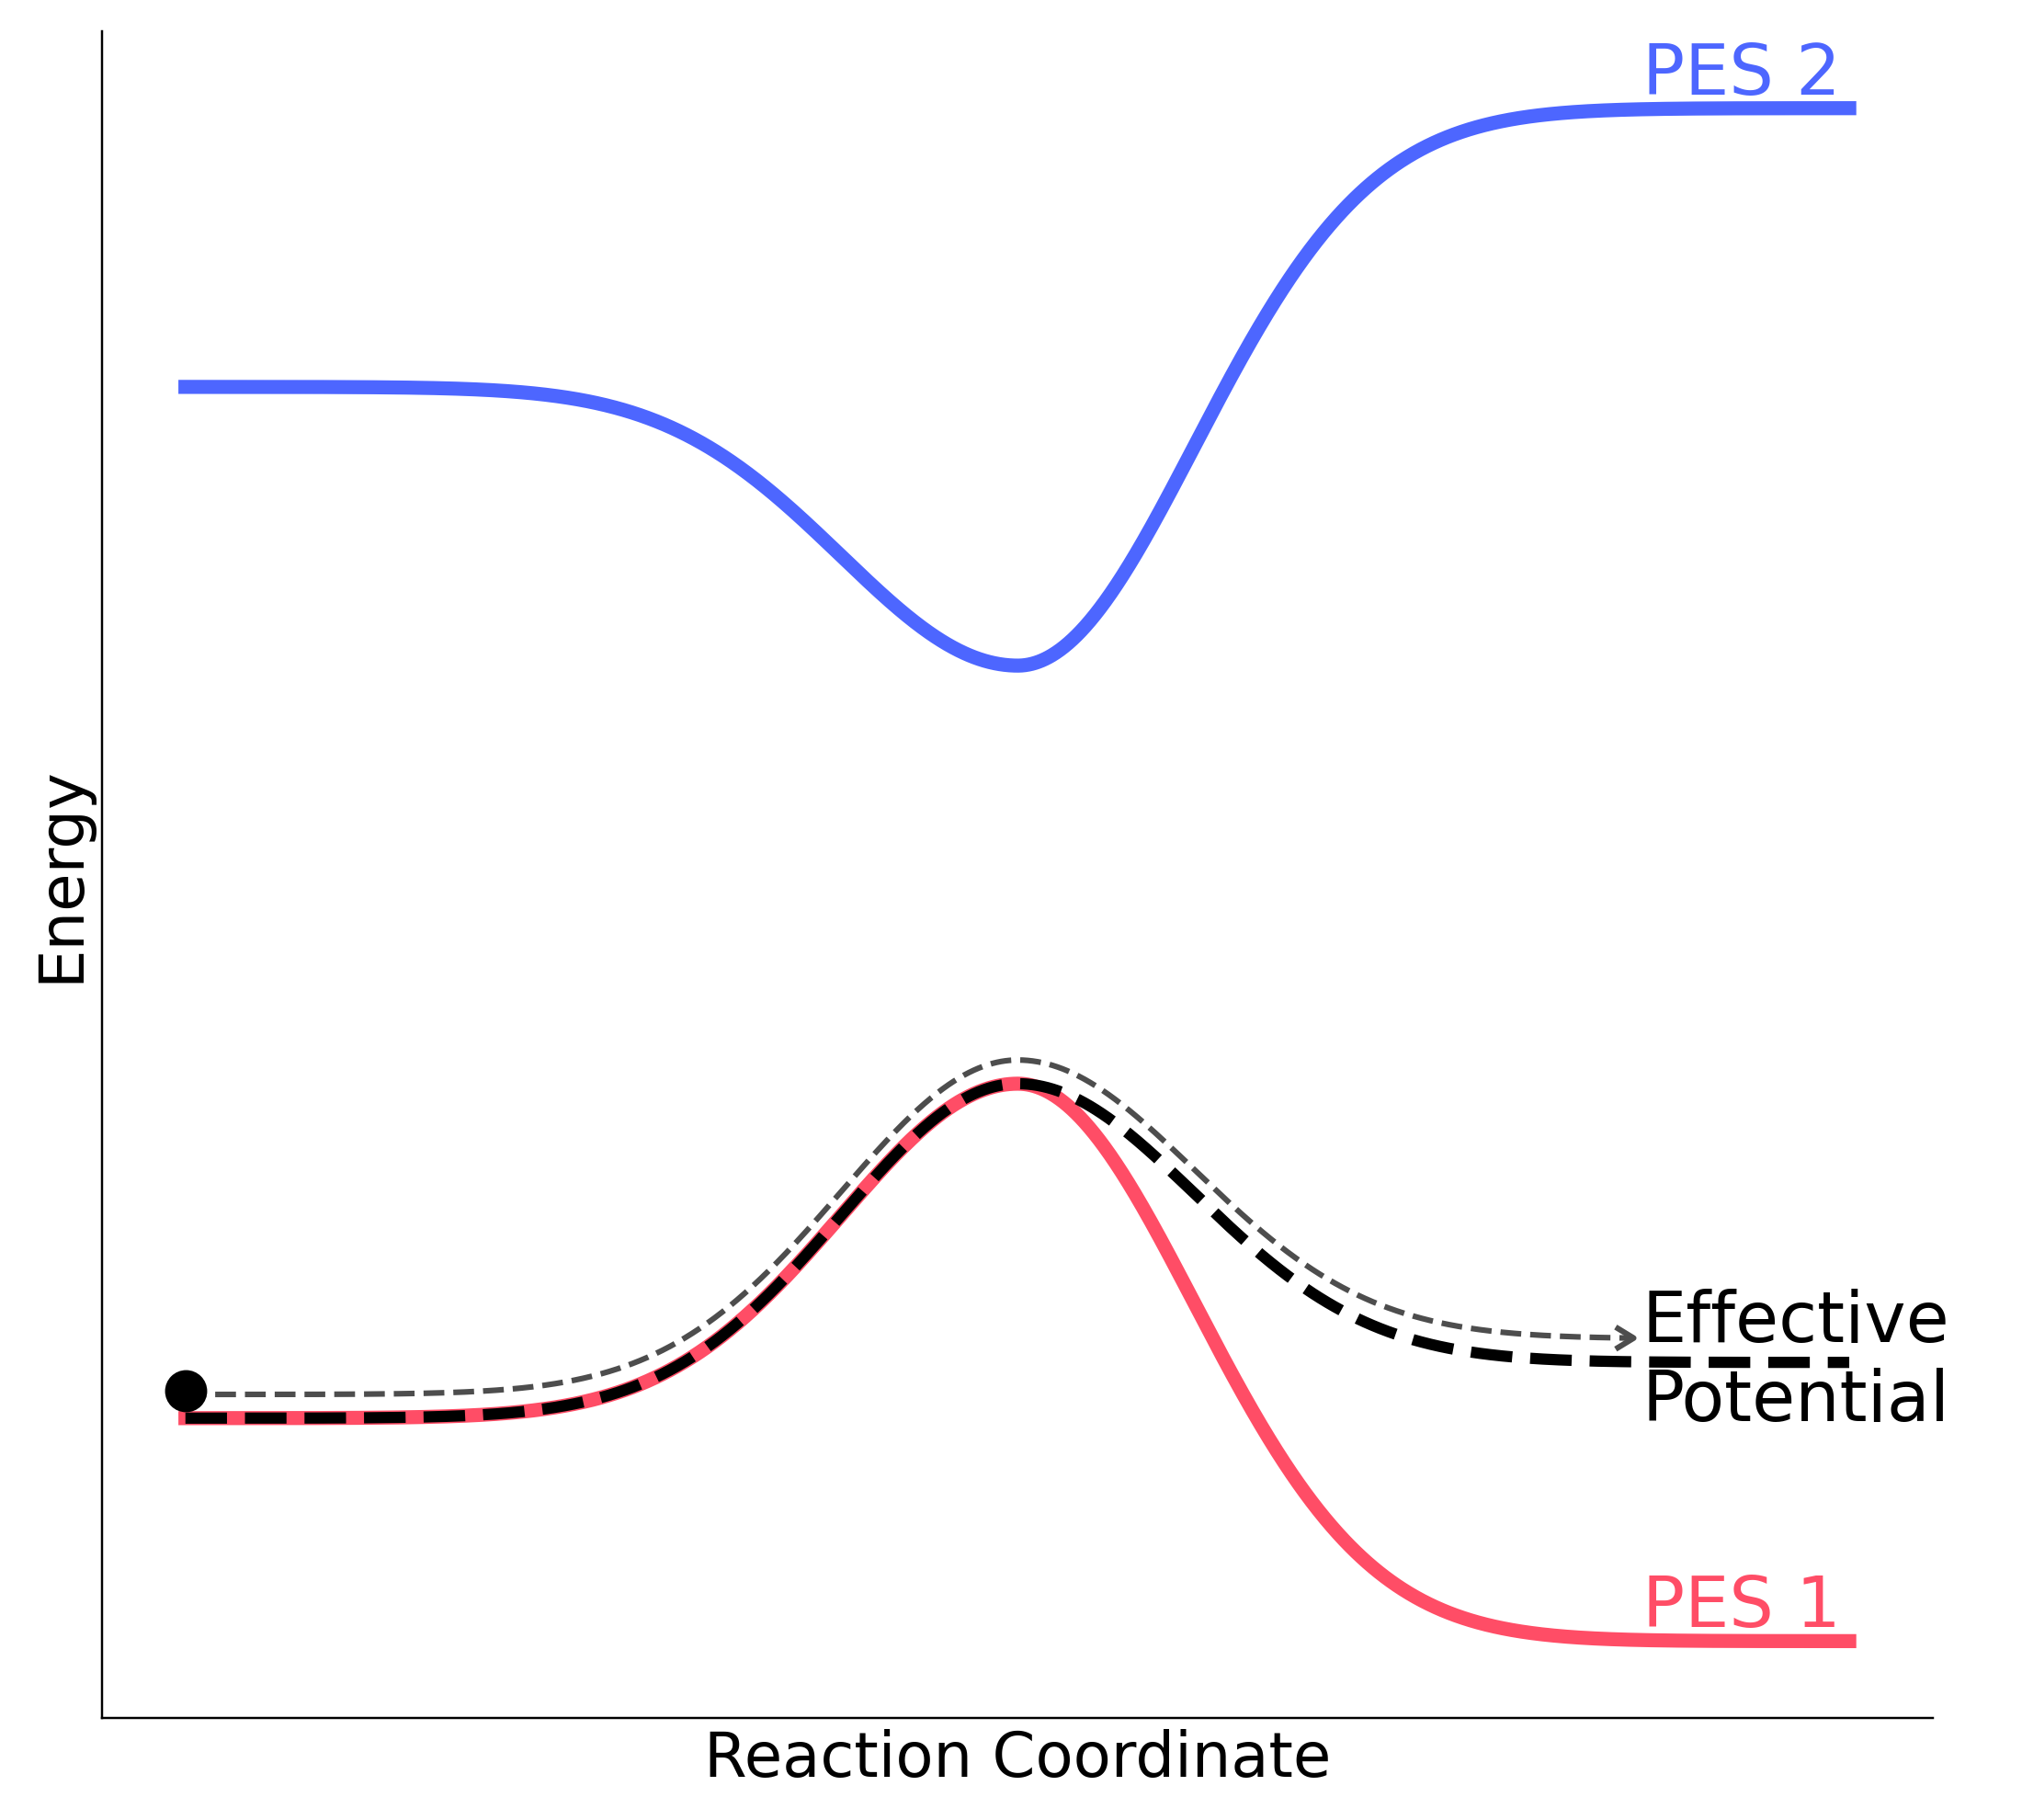
\includegraphics[width=\textwidth]{./img/Eh_hop.png}
  \caption{\label{fig:Eh_diag}An example of a typical Ehrenfest simulation near an avoided crossing. The black lines represent the adiabatic potential energy surface due to the ground (PES 1) and excited (PES 2) state. The red line represents the population weighted average potential the nuclei travel on.}
\end{figure}
\noindent The oldest, and most intuitive, NAMD method is Ehrenfest dynamics \cite{Ehren1927}. In this technique the nuclei evolve on a single, mean potential energy surface (PES). The shape of this PES comes from a population-weighted average, hence the electronic subsystem can influence the nuclear dynamics through the PES. This is method of propagation is displayed for a simple 1D, 1 atom, 2 state system in figure \ref{fig:Eh_diag}. In this figure we initialise the adiabatic population in the ground (red) state. As the atom (black dot) progress through the reaction coordinates it feels forces equal to the negative gradient of the population-weighted average PES (dotted black line).
\\\\
The Ehrenfest equations can be rigorously derived from the time-dependent Schr\"odinger equation by expanding the full the full electronic wavefunction as a linear combination of adiabatic states as in equation \eqref{eq:BornHuangExpansion} and assuming that the nuclei's motion is determined by a single population-weighted PES. The equation for the calculation of these forces is given in equation \eqref{eq:Eh_Force}.
\begin{equation}
  \Psi(\mathbf{r}, \mathbf{R}, t) = \sum_{m} C_{m}(\mathbf{R}, t) \phi_i(\mathbf{r}, t)
  \label{eq:BornHuangExpansion}
\end{equation}
Where the full electronic wavefunction $\Psi(\mathbf{r}, \mathbf{R}, t)$ is expanded as a sum of adiabatic expansion coefficients $C_{m}$ multiplied by an adiabatic basis function $\phi_i$. The norm of the adiabatic expansion coefficients gives the probability of finding the wavefunction in state $m$.
\begin{equation}
  \mathbf{F}_{\nu}^{Ehren} = \sum_i^{N_{st}} |C_{m}|^2 \mathbf{\nabla}_{\nu} E_{m} + \sum_{m \neq n}^{N_{st}} C_{m}^{*} C_{n} (E_{n} - E_{m}) \mathbf{d}_{ij, \nu}^{ad}
  \label{eq:Eh_Force}
\end{equation}
Where the force, $\mathbf{F}$, for each atom, $\nu$ is the sum of the adiabatic population, $|C_{m}|^2$, on each state, $m$, multiplied by the gradient of the adiabatic energy of state $\mathbf{\nabla}_{\nu}E_{m}$ plus the sum over pairs of adiabatic states, $m$ and $n$, of the adiabatic expansion coefficients, $C_{m (n)}$ multiplied by the energy difference $E_{n} - E_{m}$ multiplied by the nonadiabatic coupling vector $\mathbf{d}_{ij, \nu}$ on atom $\nu$. The adiabatic energies are calculated as the eigenvalues of the hamiltonian.
\\\\
The equation for the propagation of the adiabatic expansion coefficients is given in equation \eqref{eq:Eh_Elec}.
\begin{equation}
  \im \ \hbar \dot{C}_{m} = C_{m}E_{m} -  \im \ \hbar  \sum_{n}^{N_{st}} C_{n} \sum_{\nu} \mathbf{v}_{\nu} \cdot \mathbf{d}^{ad}_{mn, \nu}
  \label{eq:Eh_Elec}
\end{equation}
We can see in this equation any mixing of electronic population between states is initially stimulated by the dot between the nonadiabatic coupling vector and the nuclear velocity, $\sum_{\nu} \mathbf{v}_{\nu} \cdot \mathbf{d}_{nm, \nu}^{ad}$. In figure \ref{fig:Eh_diag} the coupling would be highest near the middle of the figure, where the 2 PES come the closest to each other, so populations would only start mixing when the nuclei reached this point. This, and the fact that the Hamiltonian (and therefore adiabatic energies) is a function of nuclear positions, is the method of feedback from the nuclear to the electronic subsystem. 
\\\\
Although the Ehrenfest method has been applied with success in many systems \cite{Li2005Aug, Saita2012Dec, Kohen1998Sep} it has a number of key shortcomings. Namely, its inability to capture the branching of the nuclear wavefunction (as propagation occurs on only a single PES) and its poor account of the decoherence of the electronic and nuclear subsystem after an avoided crossing. Ehrenfest also violates detailed balance and prevents the thermodynamic equilibration of the system by populating all adiabatic states evenly \cite{tully_perspective:_2012, john_c._tully_nonadiabatic_nodate}. In the limit of infinite states this results in infinite electronic temperature \cite{parandekar_detailed_2006}. For this reason many people choose to use fewest switches surface hopping.

\subsection{Surface hopping}
\begin{figure}[htp]
  \includegraphics[width=\textwidth]{./img/SH_hop.png}
  \caption{\label{fig:SH_diag}An example of a typical Surface Hopping simulation near an avoided crossing. The black lines represent the adiabatic potential energy surface due to the ground (PES 1) and excited (PES 2) state. The red line represents the discontinuous effective potential the nuclei travel on.}
\end{figure}
Surface hopping was devised to circumvent the limitations of mean-field NAMD. To do this a swarm of trajectories is initialised and allowed to propagate independently throughout the system. These trajectories represent the nuclear wavepacket and can have varied paths depending on the topology of the system. The shape of the PES on each trajectory is determined by discrete, stochastic hops between adiabatic potential energy surfaces. This is demonstrated for a single trajectory in figure \ref{fig:SH_diag}. In this cartoon, the expansion coefficient is initialised with its population on the ground (red) state. As the atom travels towards the avoided crossing (region of high nonadiabatic coupling), the likelihood of a hop increases. A random number is used to decide whether the hop occurs, if it does the velocities of the nuclei are adjusted/rescaled to account for the energy difference in PES (along the direction of the NACV). This is shown towards the center of figure \ref{fig:SH_diag}. After the atom has hopped to the upper surface it experiences forces equivalent to the negative gradient of the PES. In this situation it results in the atom begin reflected at the avoided crossing. Some trajectories will hop here and some won't (depending on the coupling strength) resulting in a branching of the nuclear wavepacket. This is in contrast to Ehrenfest, where all trajectories travel along the same PES, meaning the nuclear wavepacket cannot branch.
\\\\
The propagation of the adiabatic expansion coefficients is the same as for Ehrenfest and is given in equation \eqref{eq:Eh_Elec}. This results in 2 forms of adiabatic populations, the surface population (the fraction of trajectories on each PES) and the adiabatic population (the population of the adiabatic expansion coefficients). These 2 populations should agree and when they do the system is said to obey internal consistency. The forces are given by the negative gradient of the potential energy surface the trajectory is travelling on. This is given in equation \eqref{eq:SH_force}
\begin{equation}
  \mathbf{F}_{\nu} = -\mathbf{\nabla}_{\nu} E_{i} 
  \label{eq:SH_force}
\end{equation}
Where the force on atom $\nu$ is equal to the gradient (with respect to atom $\nu$) of potential energy surface $i$.
\\\\
Although surface hopping fixes many concerns from Ehrenfest dynamics there are still caveats to be aware of. The original `fewest switches surface hopping' proposed by John Tully suffered from bad overcoherence of the nuclear and electronic subsystems. That is the electronic and nuclear motion was coupled long after the region of high non-adiabatic coupling (crossing region). There have been attempts to fix this by introducing a decoherence time, after which the adiabatic population is forced to occupy a single state (either instantly or exponentially damped). However, the parameterisation of this time isn't trivial and many methods have been proposed. A decoherence method where non active adiabatic populations are exponentially damped and the active state is adjusted to conserve the norm is used in this work. The damping time is based on Heisenberg uncertainty principle and the energy difference between the active state and the inactive states. Full details of this method are given in refs \cite{Giannini2018Crossover, Carof2017FSSH}.
\\\\
Further deficiencies of trajectory surface hopping are the fact that the hops are instant which can lead to discontinuities in the total energy. The standard methods to compensate for this is re-scaling velocities along the direction of the NACV (as mentioned previously). Due to the nuclear timestep being finite trivial crossings can be missed with propagating the system. This is because when adiabatic states become very close to each other (or even totally degenerate) the nonadiabatic coupling can form a large, sharp peak with respect to the reaction coordinate. If the nuclear timestep is too large this large peak can be completely missed leading to several artifacts. There have been various solutions proposed that are referenced in ref \cite{Carof2017FSSH, Wang2016}. In this work, I will use the self-consistent surface hopping correction introduced by Wang and Prezhdo \cite{Wang2014}.  A final shortcoming of surface hopping is that it has not been derived from first principles and cannot be guaranteed to work generally. Though, in practise, surface hopping has been widely adopted and tested on a variety of systems and its suitability for use in these has been reported and many problems have been addressed \cite{Wang2016}.
\\\\
The ongoing search to address these issues, and ultimately develop the panacea of nonadiabatic molecular dynamics techniques, has lead to a number of other techniques being developed. One of these, CTMQC, will be studied in detail in this thesis and is the semi-classical limit of the exact factorisation of the time-dependent Schr\"odinger equation.
\section{Exact Factorisation and its Semi-Classical Limit}
Exact factorisation \cite{abedi_exact_2010} involves separating the total molecular wavefunction into a nuclear component and electronic component. Where the electronic component is parametrically dependent on the nuclear coordinates, $\mathbf{R}$. This is shown below in eq \eqref{eq:exact_fact} where $\chi$ is the nuclear wavefunction and $\Phi$ is the electronic one.
\begin{equation}
 \Psi(\mathbf{R}, \mathbf{r}, t) = \Phi_{\mathbf{R}}(\mathbf{r}, t) \chi(\mathbf{R}, t)
 \label{eq:exact_fact}
 \end{equation}
 In the above equation (and throughout this report) I will denote nuclear coordinates and electronic coordinates $\mathbf{R}$ and $\mathbf{r}$ respectively. The nuclear and electronic wavefunctions then obey separate, but coupled, time-dependent Schr\"odinger equations for spatial and temporal evolution. In this report, I will be focussing on the semi-classical limit of these equations, named Coupled-Trajectory Mixed Quantum-Classical Molecular Dynamics (CTMQC), and give results of a combination of this and the AOM method explained in appendix \ref{ap:AOM}.
\\\\
The equations for the evolution of the electronic and nuclear wavefunctions in the exact factorisation \cite{abedi_exact_2010} are given below:
\begin{align}
  \im\hbar \frac{\delta}{\delta t} \Phi_{\mathbf{R}}(\mathbf{r}, t) &= \left( \hat{H}_{BO} + \hat{U}_{en}\left[ \Phi_{\mathbf{R}}, \chi\right] - \epsilon(\mathbf{R}, t) \right) \Phi_{\mathbf{R}} (\mathbf{r}, t)
  \label{eq:electronic_exact}
\\
\im\hbar \frac{\delta}{\delta t} \chi (\mathbf{R}, t) &= \left( \sum_{\nu = 1}^{N_{n}} \frac{[-\im\hbar\nabla_{\nu} + \mathbf{A}_{\nu}(\mathbf{R}, t)]^2}{2 M_{\nu}} + \epsilon(\mathbf{R}, t)\right) \chi (\mathbf{R}, t)
  \label{eq:nuclear_exact}
\end{align}
Where $\hat{H}_{BO}$ is the Born-Oppenheimer Hamiltonian, that is $\hat{T}_{e} + \hat{W}_{ee} + \hat{W}_{nn} + \hat{V}_{en}$. Where $\hat{T}_{e}$ is the electronic kinetic energy operator, $\hat{W}_{ee/nn}$ is the electron-electron/nuclei-nuclei interaction and $V_{en}$ is the electronic-nuclear potential.
\\\\
The $\hat{U}_{en}$ is an electronic-nuclear coupling operator (ENCO). This is defined as \begin{equation}
  \hat{U}_{en}[\Phi_{\mathbf{R}}, \chi] = \sum_{\nu=1}^{N_{nuc}} \frac{1}{M_{\nu}} \left[ \frac{\left[-i \hbar \nabla_{\nu} - \mathbf{A}_{\nu}(\mathbf{R}, t) \right]^2}{2} + \left( \left. \left. \frac{-i\hbar \nabla_{\nu} \chi}{\chi} + \mathbf{A}_{\nu}(\mathbf{R, t})\right)\right( -i\hbar\nabla_{\nu} -            \mathbf{A}_{\nu}(\mathbf{R}, t)\right) \right]
  \label{eq:ENCO}
\end{equation}
\\
Where the $\mathbf{A}_{\nu}$ is a time-dependent vector potential (TDVP), given by $\left\langle \Phi_{\mathbf{R}}(t) \right\vert \left. - i \hbar \nabla_{\nu} \Phi_{\mathbf{R}} \right\rangle_{\mathbf{r}}$ and $M_{\nu}$ is the mass of nuclei $\nu$.
Finally $\epsilon(\mathbf{R}, t)$ is a time-dependent scalar potential energy surface (TDPES), given by $\langle \Phi_{\mathbf{R}}(t) \vert \hat{H}_{BO} + \hat{U}_{en}^{coup} - i\hbar \frac{\delta}{\delta t} \vert \Phi_{\mathbf{R}}(t) \rangle_{\mathbf{r}}$.
\\
\begin{figure}[htp]
  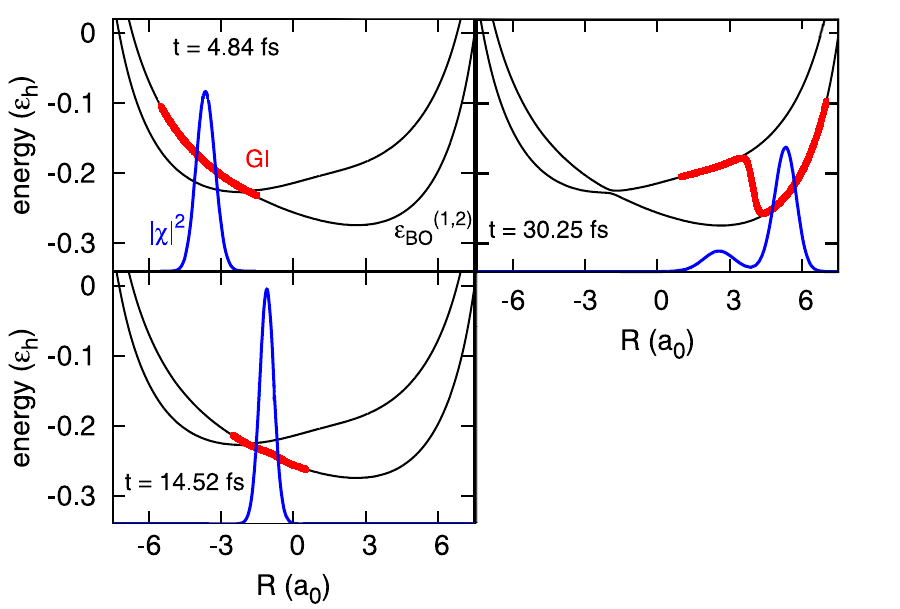
\includegraphics[width=\textwidth]{./img/CTMQC/nuclear_splitting_TDPES.png}
  \caption{A demonstration of how the TDPES can cause the splitting of the nuclear wavepacket in non-adiabatic regions. The red line represents the TDPES and the blue is the nuclear density. Figure adapted from Agostini, 15 \cite{agostini_exact_2015} \label{fig:step_TDPES}}
\end{figure}
\\
The effects of the TDPES, TDVP and the ENCO have been investigated in multiple works \cite{agostini_semiclassical_2015, agostini_exact_2015, agostini_mixed_2013, abedi_dynamical_2013, Min2014Dec}. The TDPES and TDVP are both responsible for the evolution of the system
\cite{agostini_semiclassical_2015}. The TDPES provides exact classical forces on the nuclei. In fact, an alternative independent-trajectory semi-classical scheme has been investigated using these exact forces \cite{agostini_exact_2015}. This found the TDPES is responsible for the splitting of the nuclear wavepacket in regions of high non-adiabaticity by taking the shape of a step function between the 2 adiabatic potentials. This is demonstrated in figure \ref{fig:step_TDPES}, which was adapted from an image in Agostini, 15 \cite{agostini_semiclassical_2015}. We can see the as the simulation progresses the initial nuclear density (blue curve) becomes split when the TDPES (red curve) forms a sharp step. This occurs just after the avoided crossing region. The 2 ends of the nuclear density then feel different forces from the 2 potential energy surfaces and evolve separately. Finally the electronic-nuclear coupling operator (ENCO) is responsible for other non-adiabatic effects in the system such as electronic nonadiabatic transitions and decoherence \cite{agostini_semiclassical_2015}.
\section{Approximations leading to CTMQC}
\label{sect:CTMQC_Approx}
Starting from the exact factorisation equations, 5 approximations have been made to derive the CTMQC equations. These are discussed in detail in Ref. \cite{agostini_quantum-classical_2016}. In the interest of completeness I have summarised them below.
\subsection{Classical Nuclei}
Techniques that include nuclear quantum effects (NQEs); such as multiple spawning \cite{Martnnez*2005Oct}, ring-polymer surface hopping \cite{Shakib2017Jul} and nonadiabatic Bohmian dynamics \cite{Curchod2011Feb, Tavernelli2013Apr} although extremely accurate, cannot be applied to hundreds or thousands of molecules, due to their high computational cost. Further, in many systems of interest NQEs are negligible, especially at room temperature. For this reason the classical limit of the nuclear Schr\"odinger equation \eqref{eq:nuclear_exact} is taken when deriving the CTMQC equations.
\subsection{Neglect the ENCO in the TDPES}
The electron-nuclei coupling operator is omitted in the expression for the time-dependent potential energy surface. This is justified as the first term ($\left[-i \hbar \nabla_{\nu} - \mathbf{A}_{\nu}(\mathbf{R}, t) \right]^2$) contains a second order derivative which is expensive to calculate and has a neglible effect compared to the second term in the ENCO \cite{Scherrer2015Aug}. However, the rest of the ENCO is equal to zero when averaged over $\Phi_{\mathbf{R}}(\mathbf{r},t)$ so it does not contribute to the TDPES.
\subsection{Derivative of the Adiabatic Coefficients}
The derivative of the adiabatic coefficients appears in the electronic evolution equations. However, we can re-write the derivative of the adiabatic coefficients in terms of their modulus and phase:
\begin{equation}
  \nabla_{\nu} C_{l}^{(I)}(t) = \left[ \underbrace{\frac{\nabla_{\nu} |C_{l}^{(I)}(t)|}{|C_{l}^{(I)}(t)|}}_{(\text{Term 1})} + \underbrace{\frac{i}{\hbar} \nabla_{\nu} \gamma_{l}^{(I)}(t)}_{(\text{Term 2})}\right] C_{l}^{(I)}(t)
\end{equation}
It has been found that the first term is negligible compared to the second \cite{abedi_dynamical_2013, agostini_mixed_2013, agostini_exact_2015} so it doesn't need to be calculated and we can remove it. It was also assumed that the NACVs are localised in space meaning that, after some algebra, the spatial derivative of the adiabatic coefficient can be written as:
\begin{equation}
  \nabla_{\nu} C_{l}^{(I)}(t) = \frac{i}{\hbar} \nabla_{\nu} \gamma_{l}^{(I)}(t) C_{l}^{(I)}(t) = -\frac{i}{\hbar} \int^{t} dt' \nabla_{\nu} \epsilon_{l}^{(I)} C_{l}^{(I)}(t) = -\frac{i}{\hbar} \mathbf{f}_{l}^{(I)} C_{l}^{(I)}(t)
  \label{eq:hist_force}
\end{equation}
Where $\epsilon_{l}^{(I)}$ is the energy of the l$^{th}$ adiabatic potential energy surface for trajectory I, $C_{l}^{(I)}$ is the adiabatic expansion coefficient for state l and trajectory I. The $\mathbf{f}_{l}^{(I)}$ is the time-integrated adiabatic force (adiabatic momentum).
\subsection{Gaussian Nuclear Wavepackets}
In order to calculate the quantum momentum -the new term in CTMQC. Knowledge of the nuclear distribution is needed. However, as we treat the nuclei as point particles we need to re-construct the nuclear density from the atomic positions. This is done by smoothing out the atomic positions by placing a gaussian of width $\sigma$ centered on each atomic position and combining these gaussians to produce the final nuclear density. This introduces an empirical parameter ($\sigma$) which will be discussed later in this thesis. It should be noted, the nuclei are still propagated classically, the width parameter is only used in the calculation of the quantum momentum.
\subsection{Seperating the Effects of Decoherence and NACVs}
So as to not introduce any population transfer (due to the quantum momentum) when the NACV is zero a fifth approximation has been introduced. Namely the quantum momentum depends on pairs of states -l,k. This enables the separation of the `competing' effects of the NACV and the Quantum Momentum.
\section{The CTMQC equations}
\subsection{Adiabatic Basis}
\label{sec:ad_eqns}
The equations for the propagation of the classical nuclei and the expansion coefficients in the CTMQC framework in the adiabatic basis are given below:
\begin{dmath}
  \dot{\mathbf{P}}_{\nu}^{(I)} =
  -\overbrace{
     \sum_{k} |C_{k}^{(I)}|^2 \nabla_{\nu}\epsilon_{k}^{(I)}
     - \sum_{k,l} C_{l}^{(I)} C_{k}^{* (I)} \left(\epsilon_{k}^{(I)}  - \epsilon_{l}^{(I)}   \right)
  }^{\text{Ehrenfest}}
  \\
  \underbrace{
    - \sum_{l,k} |C_{l}^{(I)}|^2 \left( \sum_{\nu'=1}^{N_n}    \frac{2}{\hbar M_{\nu'}} \mathcal{Q}_{lk, \nu}^{(I)} \cdot    \mathbf{f}_{l, \nu}^{(I)} \right)\left[ |C_{k}^{(I)}|^2    \mathbf{f}_{k,\nu}^{(I)} - \mathbf{f}_{l,\nu}^{(I)} \right]
  }_{\text{Quantum Momentum}}
    \label{eq:nuc_adiab}
\end{dmath}

\begin{dmath}
  \dot{C}_{l}^{(I)} =
  \overbrace{
    -\frac{i}{\hbar} \epsilon_l^{(I)} C_{l}
    - \sum_k C_k^{(I)} d_{lk}^{ad \ (I)}
  }^{\text{Ehrenfest}}
  \\
  \underbrace{
    - \sum_{\nu=1}^{N_n}\sum_{k} \frac{\mathcal{Q}_{lk, \nu}^{(I)}}{\hbar M_\nu} \cdot \left[ \mathbf{f}_{k,\nu}^{(I)} - \mathbf{f}_{l,\nu}^{(I)} \right] |C_{k}^{(I)}|^2 C_{l}^{(I)}
  }_{\text{Quantum Momentum}}
  \label{eq:elec_adiab}
\end{dmath}
Where the $\epsilon_k$ term is the potential energy on the k$^{th}$ potential energy surface. $C_l$ is the adiabatic expansion coefficient corresponding to the l$^{th}$ state. The sum over k and l indicates a sum over all states, the (I) superscript is a replica index and the $\nu$ is an atom index. $M_{\nu}$ is  the nuclear mass and $d_{lk}^{ad (I)}$ represents the non-adiabatic coupling element (in the adiabatic basis) between adiabatic states l and k.
The 2 new terms in this scheme not seen in other NAMD methods are the $\mathcal{Q}_{lk, \nu}^{(I)}$ and the $\mathbf{f}_{k, \nu}^{(I)}$. These are the quantum momentum and the adiabatic momentum. The adiabatic momentum term is defined in equation \eqref{eq:hist_force} this keeps a record of the previous forces on each adiabatic state in the system. The quantum momentum term couples the trajectories together (making this a coupled-trajectory scheme). Together the history dependent force and quantum momentum are responsible for the decoherence in the `Quantum Momentum' parts of the above equations \cite{gossel_coupled-trajectory_2018}. Notably, although these equations have been derived from the exact factorisation equations separately from Ehrenfest they do contain the Ehrenfest equations within them (marked `Ehrenfest'). This scheme can therefore be seen as an Ehrenfest scheme with a correction that captures branching of the nuclear wavefunction and decoherence within it.
\\\\
We can also see in equation \eqref{eq:elec_adiab} if we are in a pure adiabatic state i.e. all population on a single adiabatic state, there is no contribution from the quantum momentum part of the equations. In this scenario the evolution equations become simply Ehrenfest equations. For example, if all the population is localised on a single adiabatic state then the term $|C_{k}^{(I)}|^2 C_{l}$ is only non-zero when $l = k$. However, when $l = k$, the term $\left[ \mathbf{f}_{k,\nu}^{(I)} - \mathbf{f}_{l,\nu}^{(I)} \right]$ is zero as $\mathbf{f}_{k,\nu}^{(I)} = \mathbf{f}_{l,\nu}^{(I)}$.
Therefore, the quantum momentum term can be seen to only kick in when there is a mixing of adiabatic states. In the adiabatic formulation of these equations it is the adiabatic NACV $\mathbf{d}_{lk, \nu}^{ad, (I)}$ that is responsible for the initial mixing of the populations from pure adiabatic states.
 \subsection{Calculating the Quantum Momentum \label{sec:calc_QM}}
 \label{sect:QM_Calc}
 The technique for calculating the quantum momentum term is outlined in detail in the SI of min, 17 \cite{min_ab_2017}. The original equations given in Agostini, 16\cite{agostini_quantum-classical_2016} present a quantum momentum term without state indices (l,k). This, due to approximations made in the derivation of CTMQC, results in population transfer even when the non-adiabatic couplings between states are zero. Therefore, Agostini et al enforced this condition with the pair-wise state dependence on the quantum momentum. The quantum momentum is defined in equation \eqref{eq:QM_def} as:
\begin{equation}
  \mathcal{Q}_{\nu}^{(I)} = \frac{-\hbar \nabla_{\nu} |\chi^{(I)}|}{|\chi^{(I)}|} \frac{-\hbar \nabla_{\nu}                            |\chi^{(I)}|^2}{2|\chi^{(I)}|^2}
  \label{eq:QM_def}
\end{equation}
In order to reconstruct the nuclear density, Gaussian distributions are used as in equation \eqref{eq:NuclDens} below:
\begin{equation}
	|\chi^{(I)}(t)|^2 = \frac{1}{N_{tr}} \sum_{J=1}^{N_{tr}} \prod_{\nu=1}^{N_n} g_{\sigma_{\nu}^{(J)}(t)} \left(\mathbf{R}_{\nu}^{(I)}(t) - \mathbf{R}_{\nu}^{(J)}(t)\right)
	\label{eq:NuclDens}
\end{equation}
Where, $N_{tr}$ is the number of trajectories, $N_{n}$ is the number of atoms, $\sigma_{\nu}^{(J)}(t)$ is a time-dependent width parameter for each gaussian $g$ and $\mathbf{R}_{\nu}^{(J)}$ represents the atomic position of atom $\nu$ on trajectory $J$.
\\\\
This results in a linear expression for the quantum momentum.
The full details of the derivation are given in the supplementary information of Min, 17 \cite{min_ab_2017}. The resulting linear expression for the quantum momentum is given below:
\begin{equation}
  \mathcal{Q}_{lk, \nu}^{(I)} = \alpha_{\nu}^{(I)} \mathbf{R}_{\nu}^{(I)} - \mathbf{R}_{lk, \nu}
  \label{eq:QM_lin}
\end{equation}
Where $\mathbf{R}_{\nu}^{(I)}$ are the nuclear coordinates on trajectory I on atom $\nu$. The $\alpha_{\nu}^{(I)}$ term is a weighted  average over trajectories of the product of the gaussian's assigned to each atomic coordinate, i.e:
\begin{equation}
  \alpha_{\nu}^{(I)} = \sum_{J}^{N_{tr}} \frac{\hbar \prod_{\nu'} g_{\sigma_{\nu'}^{(J)}(t)}\left(\mathbf{R}_{\nu'}^{(I)}(t) -         \mathbf{R}_{\nu'}^{(J)}(t)\right)}   {2 \sigma_{\nu}^{(J)}(t)^2\sum_{K}^{N_{tr}}\prod_{\nu'}                                           g_{\sigma_{\nu'}^{(K)}(t)}\left(\mathbf{R}_{\nu'}^{(I)}(t) - \mathbf{R}_{\nu'}^{K)}(t)\right)}
  \label{eq:alpha}
\end{equation}
Along with the $\mathbf{R}_{lk, \nu}$ term the $\alpha_{\nu}^{(I)}$ performs the job of coupling the trajectories together. The $\mathbf{R}_{lk, \nu}$ term also given in the SI of Min, 17\cite{min_ab_2017} is defined for each Cartesian dimension as:
\begin{equation}
  R_{lk, \nu} = \sum_{I}^{N_{tr}} R_{\nu}^{(I)}(t) \alpha_{\nu}^{(I)}(t) \frac{|C_{k}^{(I)}(t)|^2 |C_{l}^{(I)}(t)|^2 \left( f_{k,      \nu}^{(I)}(t) - f_{l, \nu}^{(I)}(t) \right)}{\sum_{J} |C_{k}^{(J)}(t)|^2 |C_{l}^{(J)}(t)|^2 \left( f_{k, \nu}^{(J)}(t) - f_{l,         \nu}^{(J)}(t) \right)}
  \label{eq:Rlk}
\end{equation}
Where the bold notation for vectors has been replaced by normal font. This means that this equation applies to each Cartesian dimension independently. Further, in this expression $R_{lk, \nu}$ is symmetric, $R_{lk} = R_{kl}$ meaning that $Q_{lk} = Q_{kl}$. It is also undefined on the diagonals as the denominator is 0, diagonal values are therefore set to 0. At first sight, the $R_{lk}$ term seems to be another weighted average. However, this isn't quite the case as the denominator can be negative. This causes equation \eqref{eq:Rlk} to be very sensitive to errors in the calculation of the denominator of this fraction. Any inaccuracies can lead to the denominator approaching zero faster than the numerator causing large spikes in the quantum momentum term. This will be discussed in greater detail in the following chapters.






%In order to properly quantify the performance of organic semiconductors a key property is the charge carrier mobility. Typically, charge carrier mobilities in `good' organic semiconductors (OSCs) fall between 1-10 cm$^2$V$^{-1}$s$^{-1}$ \cite{Brown2018Mar}. Though higher mobilities, in pure crystals such as Rubrene, have been recorded in the range 15-20+ cm$^2$V$^{-1}$s$^{-1}$ \cite{Zimmerling_RubMob, Podzorov_Rubrene}. This is beyond the range of hopping model validity ($\sim$1 cm$^2$V$^{-1}$s$^{-1}$) and below that of band theory ($>$ 50 cm$^2$V$^{-1}$s$^{-1}$) \cite{yavuz_dichotomy_2017}. In this intermediate regime the charge carriers are typically not completely delocalised at the valence band edges (band regime) or localised to a single site/molecule (hopping regime) but delocalised over a few/tens of molecules \cite{giannini_crossover_2018}. Without any analytic approaches currently being valid in this regime many atomistic computational approaches have been developed to investigate the underlying charge transport mechanisms\cite{oberhofer_charge_2017}.

%The wavefunction is normally expanded as a linear combination of adiabatic or diabatic states. The nuclei and electrons can also interact. Taking account of this interaction is where these techniques differ. No one technique is perfect, the issues for surface hopping and Ehrenfest are well documented and have been discussed in detail \cite{SubotnikReview2016, Giovanni_2010_deco, Jaeger_2012_deco, Jain2016, Subotnik_2011_deco}. CTMQC is a fairly new technique and its issues are still mostly unknown. In this document I will discuss CTMQC in depth and present results from my own implementation of it as well as presenting its drawbacks. I will also compare these results to Ehrenfest and Trajectory Surface Hopping (TSH).

\chapter{CTMQC applied to the Tully Models}
\label{chap:tully_models}

The Tully models, first proposed by John Tully in 1990 \cite{tully_molecular_1990}, are a collection of simple 1 dimensional model systems. They were designed to be simple enough to obtain accurate quantum results to benchmark new nonadiabatic molecular dynamics (NAMD) methods against. Originally there were 3, 1 dimensional, 1 atom models. However, in this work an extra model has been introduced with parameters taken from Gossel, 18 \cite{gossel_coupled-trajectory_2018}. This is to allow a full comparison of my implementation of CTMQC with the literature. In this chapter my implementation of CTMQC will be tested using these model systems and by comparing my results with those in the literature.
\\\\
In each of the Tully models the (diabatic) Hamiltonian is a function of nuclear positions and is a 2$\times$2 matrix that takes the form:
\begin{equation}
  \hat{H} = \frac{\ \hat{P} ^2}{2M} + \left(
                                              \begin{array}{cc}
                                                H_{11}(\mathbf{R}) & H_{12}(\mathbf{R}) \\
                                                H_{21}(\mathbf{R}) & H_{22}(\mathbf{R})
                                              \end{array}
                                         \right)
\end{equation}
The nuclear mass has been set to 2000 a.u.. This was set to be very close to the proton's mass of 1836 a.u. so we can expect significant quantum effects that classical theory couldn't replicate. The values of the Hamiltonian matrix elements are set to produce systems that resemble common features in a typical nonadiabatic simulation such as avoided crossings and regions of extended coupling. The parameters used in each systems' Hamiltonian where taken from Gossel, 18 \cite{gossel_coupled-trajectory_2018} in order to compare the 2 implementations. These can be found in appendix \ref{ap:tully_params}.
\\\\
In order to propagate dynamics in the adiabatic basis we need to calculate various quantities from the hamiltonian at each timestep. These are, for Ehrenfest, the (adiabatic) nonadiabatic coupling vector ($\mathbf{d}_{lk}^{(I)}$) and the adiabatic energies ($E_{l}^{(I)}$). In the full CTMQC simulations we must also calculate the adiabatic momentum term $\mathbf{f}_{l}^{(I)}$ from the Hamiltonian. The adiabatic energies are the eigenvalues of the Hamiltonian. The adiabatic NACV can be calculated via a finite difference method and equation \eqref{eq:NACV_def} below.
\begin{equation}
  \mathbf{d}_{lk}^{(I)} = \langle \psi_{l}^{(I)} | \nabla \psi_k^{(I)} \rangle
  \label{eq:NACV_def}
\end{equation}
Where $\psi_{l}^{(I)}$ is the adiabatic electronic basis function for adiabatic state l. This is given by the eigenvector of the Hamiltonian, on replica I, corresponding to state l. Illustrations of these 2 properties can be found below in fig \ref{fig:tully_schematics} for each of the 4 models systems.
\begin{figure}[H]
  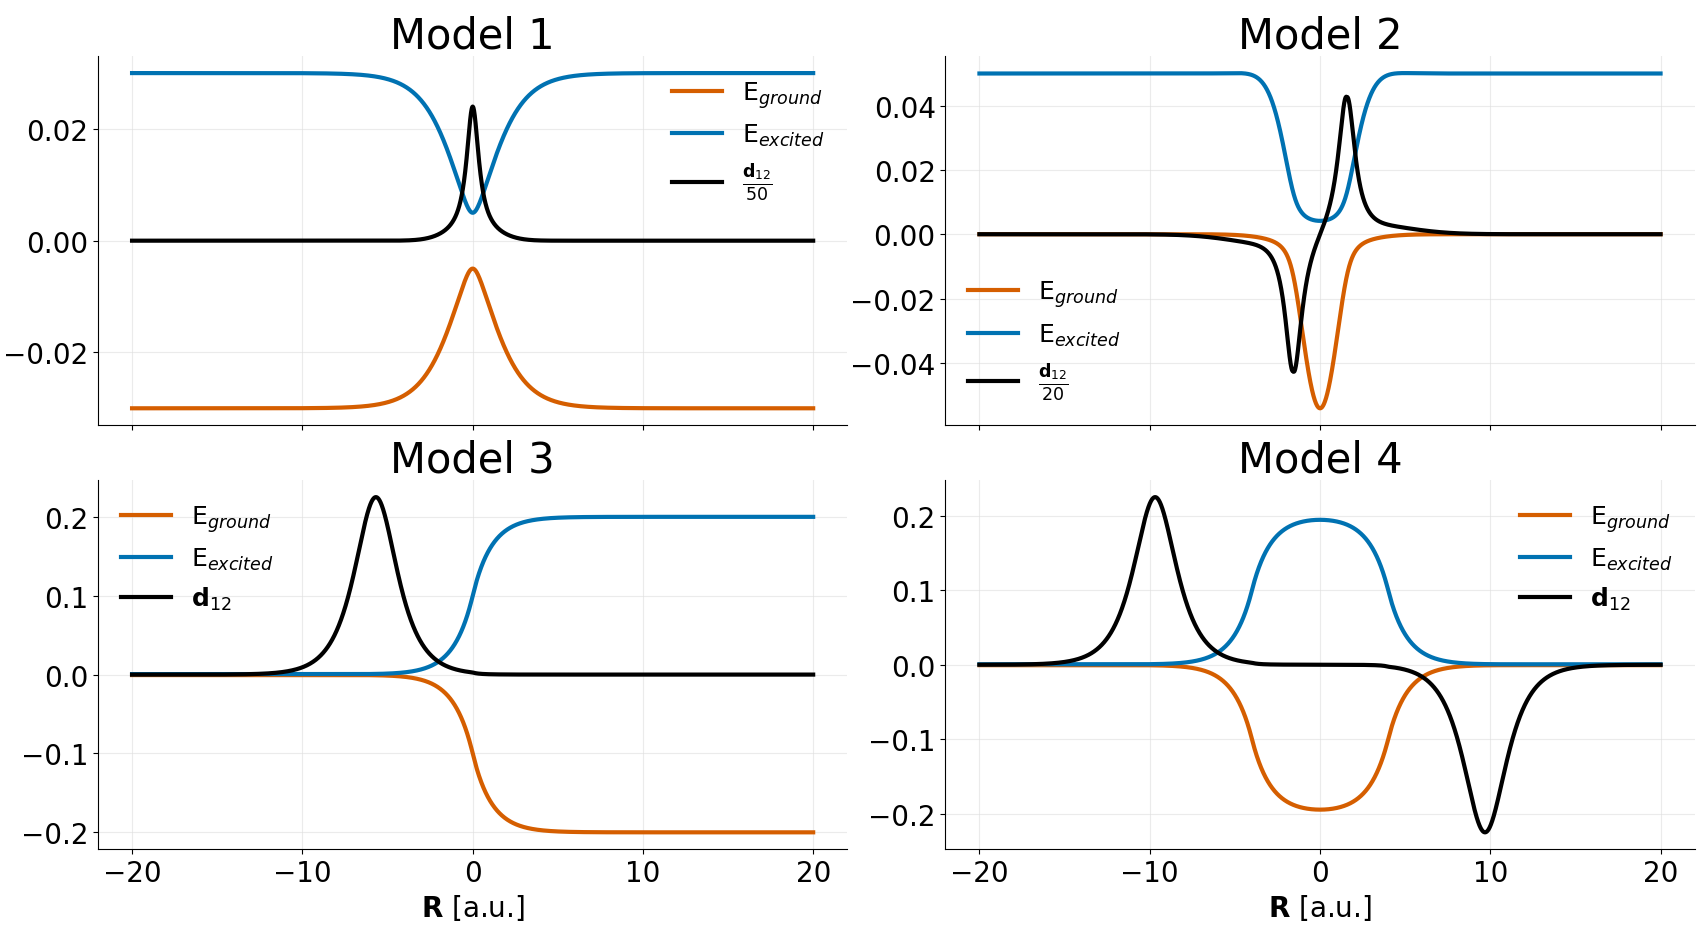
\includegraphics[width=\textwidth]{Chapter_tullyModels/model_schematics.png}
  \caption{\label{fig:tully_schematics}Adiabatic potential energy surfaces (orange and blue) and element 1, 2 of the nonadiabatic coupling vector (black) for the 4 model systems. For parameters see appendix \ref{ap:tully_params}.}
\end{figure}
\newpage
\noindent In order to initialise the simulations coordinates and velocities were sampled from the Wigner phase-space distribution of a gaussian nuclear wavepackets given by equation \eqref{eq:initial_nucl_wp}. A derivation of this can be found in appendix \ref{ap:Wigner}. The nuclear positions/velocities were then propagated using a velocity verlet algorithm and the adiabatic expansion coefficients were propagated using a 4$^{th}$ order Runge-Kutta method.
\begin{equation}
  \chi(R, 0) = \frac{1}{(\pi \mu^2)^{\frac{1}{4}}} e^{-\frac{(R - R_0)^2}{2 \mu^2} + \im k_0 (R - R_0) }
  \label{eq:initial_nucl_wp}
\end{equation}
The adiabatic coefficients were initialised purely on the ground state and the initial width of the nuclear wavepacket was set to $\mu = \sqrt{2}$ bohr. 2 values of initial momenta $k_0$ were chosen for each model, 1 low value and another higher one. Full details of all input parameters can be found in appendix \ref{ap:tully_params}. I have implemented a serial version of CTMQC acting on Tully's toy model systems and real molecular systems using couplings derived from the analytic overlap method \cite{gajdos_ultrafast_2014} within the software package CP2K \cite{cp2k} and for Tully's model systems as standalone python code. These are accessible publicly via github repositories at: \href{https://github.com/95ellismle}{github.com/95ellismle}. This work will only focus on results from the CP2K implementation as we will later see this code extended and applied to systems of real Ethylene molecules.

\section{Testing My Implementation -Ehrenfest}
The motivation behind implementing CTMQC for the Tully models was to serve as a verifiable base for later extensions, such as integrating CTMQC within the fragment-orbital based (FOB) \cite{spencer_fob-sh:_2016} framework which will be discussed in a later chapter \cite{chap:molecular_systems}. Using such simple systems will also help to clarify how each new parameter works and make testing and debugging easier. As well as many numerical tests on individual terms in the equations,  I have implemented some physical tests on the overall system dynamics. In this section, I will outline the key tests I have performed on the Ehrenfest propagation and will include the full details of the full CTMQC propagation in the following section.
\\\\
In all the simulations when the Tully models are referenced they will refer to those parameters given in appendix \ref{ap:tully_params}. Reference to a high momentum Tully model simulation is a reference to that model with initial momenta being sampled from the Wigner distribution of the higher of the 2 initial momenta given in appendix \ref{ap:tully_params}.

\subsection{Norm Conservation}
\label{sect:normConsEhren}
\begin{figure}[ht]
	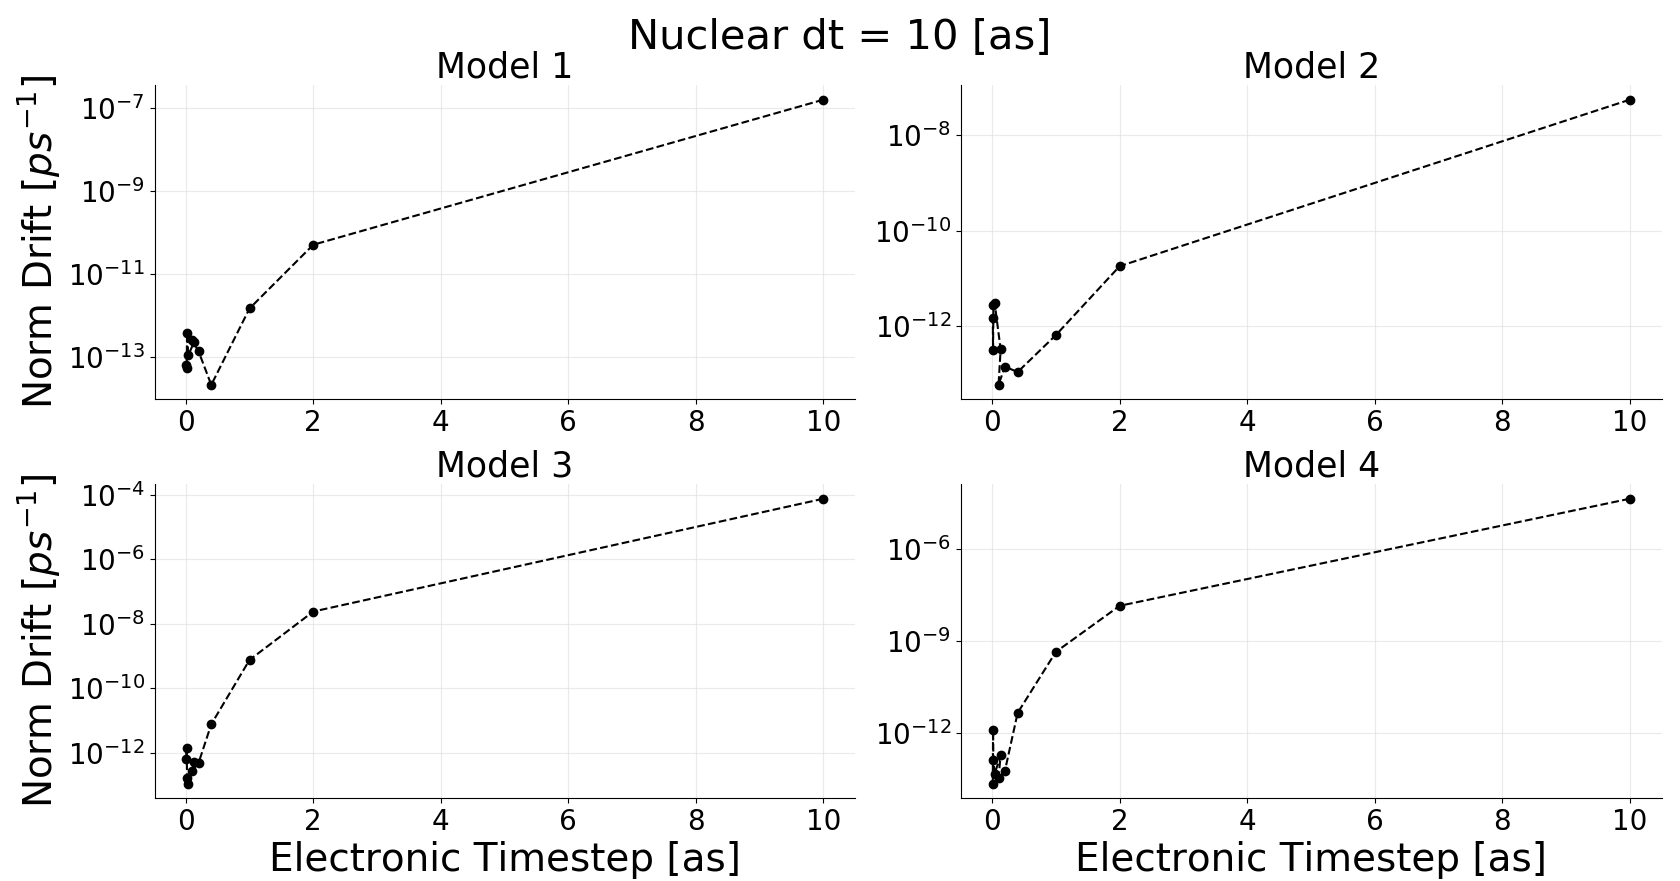
\includegraphics[width=\textwidth]{/home/matt/Documents/PhD/PhD_Thesis/img/CTMQC/TullyModels/Ehren_Norm_Conservation.png}
	\caption{\label{fig:EhrenNormCons}The norm conservation averaged over all replicas for Ehrenfest simulations with various electronic timesteps for each Tully model using a initial high momenta.}
\end{figure}
\noindent In appendix \ref{ap:norm_cons}, it is shown that the norm of the adiabatic expansion coefficients should be conserved throughout the simulation. To test the conservation of the norm of the expansion coefficients Ehrenfest simulations were ran with various electronic timesteps (with a constant nuclear timestep) for each of the 4 high momentum Tully models. The high momentum Tully models were chosen as they are expected to provide a worst case scenario of the norm conservation, due to populations changing more quickly leading to reduced sampling. As can be seen in figure \ref{fig:EhrenNormCons}, the norm of the wavefunction is conserved within numerical error ($10^{-12}$) when     using a sufficiently small timestep in every Tully model.

\subsection{Energy Conservation}
Energy conservation is a very important property in most molecular dynamics simulations. In Ehrenfest of mean-field molecular dynamics nuclei are propagated on a population-weighted mean potential energy surface, e.g. $\sum_{k}|C_{l}^{(I)}(t)|^2 = E_{eff}(t)$ \cite{EhrenEnerCons}. Kinetic energy of the classical nuclei is given by the standard formula, e.g. $\frac{1}{2} m v^2$. We can therefore write down the conserved quantity as defined below in equation \eqref{eq:EhrenfestEnergyConservation}:
\begin{equation}
  \frac{d E}{dt} = \frac{d}{dt} \left[ \frac{1}{2} m v^2 + \sum_{k}|C_{l}^{(I)}(t)|^2 \right] = 0
  \label{eq:EhrenfestEnergyConservation}
\end{equation}
As in the norm conservation checks in section \ref{sect:normCons},  parameters from the high momentum cases were taken as initial conditions for simulations with various nuclear timesteps, this time holding the electronic timestep constant. The high momenta cases were chosen to show the worst case energy conservations. A linear line of best fit was then fitted to the data and the drift in the total energy (given in \eqref{eq:EhrenfestEnergyConservation}) was calculated from its gradient. The results of these simulations are given in figure \ref{fig:EhrenEnerCons}.
\begin{figure}[ht]
  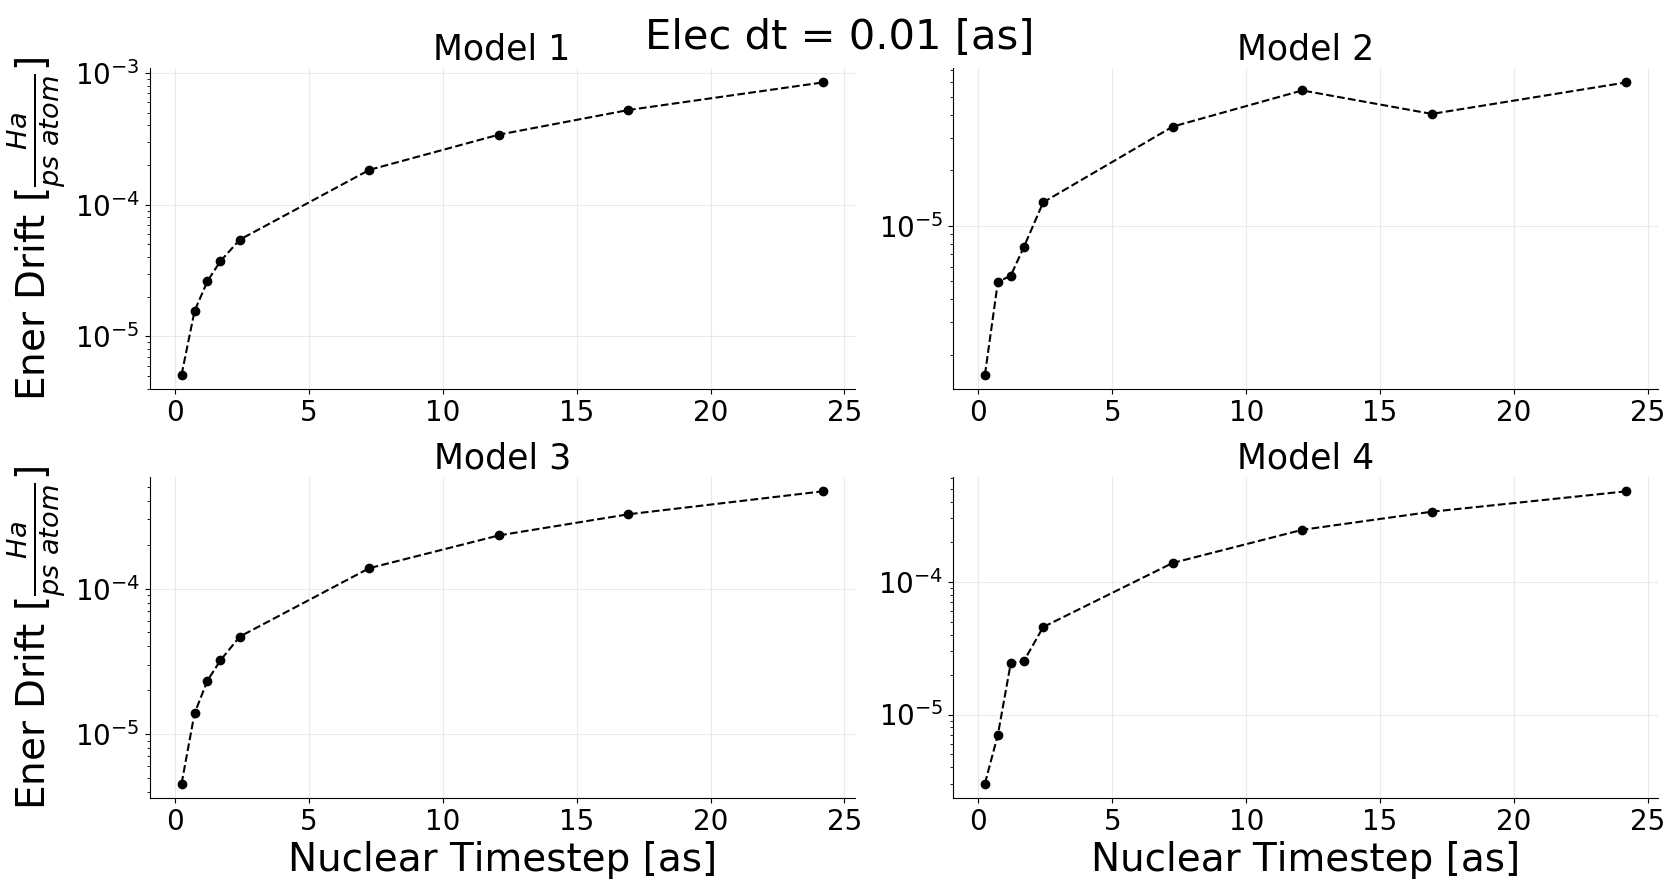
\includegraphics[width=\textwidth]{./img/CTMQC/TullyModels/Ehren_EnerCons.png}
  \caption{\label{fig:EhrenEnerCons}Energy conservation values for various nuclear timesteps for the high momentum case of each Tully model using Ehrenfest dynamics.}
\end{figure}
In figure \ref{fig:EhrenEnerCons}, we see the expected results that as the nuclear timestep is decrease the drift in the total energy also decreases. This trend validates the implementation and shows that in the limit of infinitely small timestep (and infinite computer precision) perfect energy conservation would be achieved. However, fairly small nuclear timesteps are required to achieve reasonable energy conservations. This is because the system contains only 1 atom with a mass comparable to that of Hydrogen. If one needed an improved energy conservation a higher order integrator than the velocity verlet used here may also improve results slightly.

\subsection{Comparisons To Literature}
\subsubsection{Gossel, 18 and Agostini, 16}
\label{sect:EhrenCompare}
There have been 2 papers published applying CTMQC and Ehrenfest to the Tully models \cite{gossel_coupled-trajectory_2018, agostini_quantum-classical_2016} and both contain results for the 4 Tully models shown in fig \ref{fig:tully_schematics}. The results contain data on the (ground state) adiabatic populations and a coherence indicator (shown in equation \eqref{eq:coherence_indicator}) for 16 different simulations (a low and high initial momentum simulation of Models 1, 2, 3 and 4). However, models 1 and 4 in Agostini, 16 \cite{agostini_quantum-classical_2016} used a different initial momentum so these have been omitted from the results in figure \ref{fig:LitCompEhrenTully}.
\begin{equation}
	|\rho_{12}(t)|^2 = \frac{1}{N_{tr}} \sum_{I=1}^{N_{tr}} |C_{1}^{(I)}(t)|^2 |C_{2}^{(I)}(t)|^2
	\label{eq:coherence_indicator}
\end{equation}
\\\\
In order to compare to results in the literature the same setup had to be used. In this case this meant sampling individual replicas' initial conditions (positions and momenta) from a Wigner distribution with a mean position and momenta given in appendix \ref{ap:tully_params}. The wavefunction was initialised purely on the ground state and the same integrator was used for the nuclear and electronic propagation (velocity verlet and RK4 respectively).
\begin{figure}[ht]
	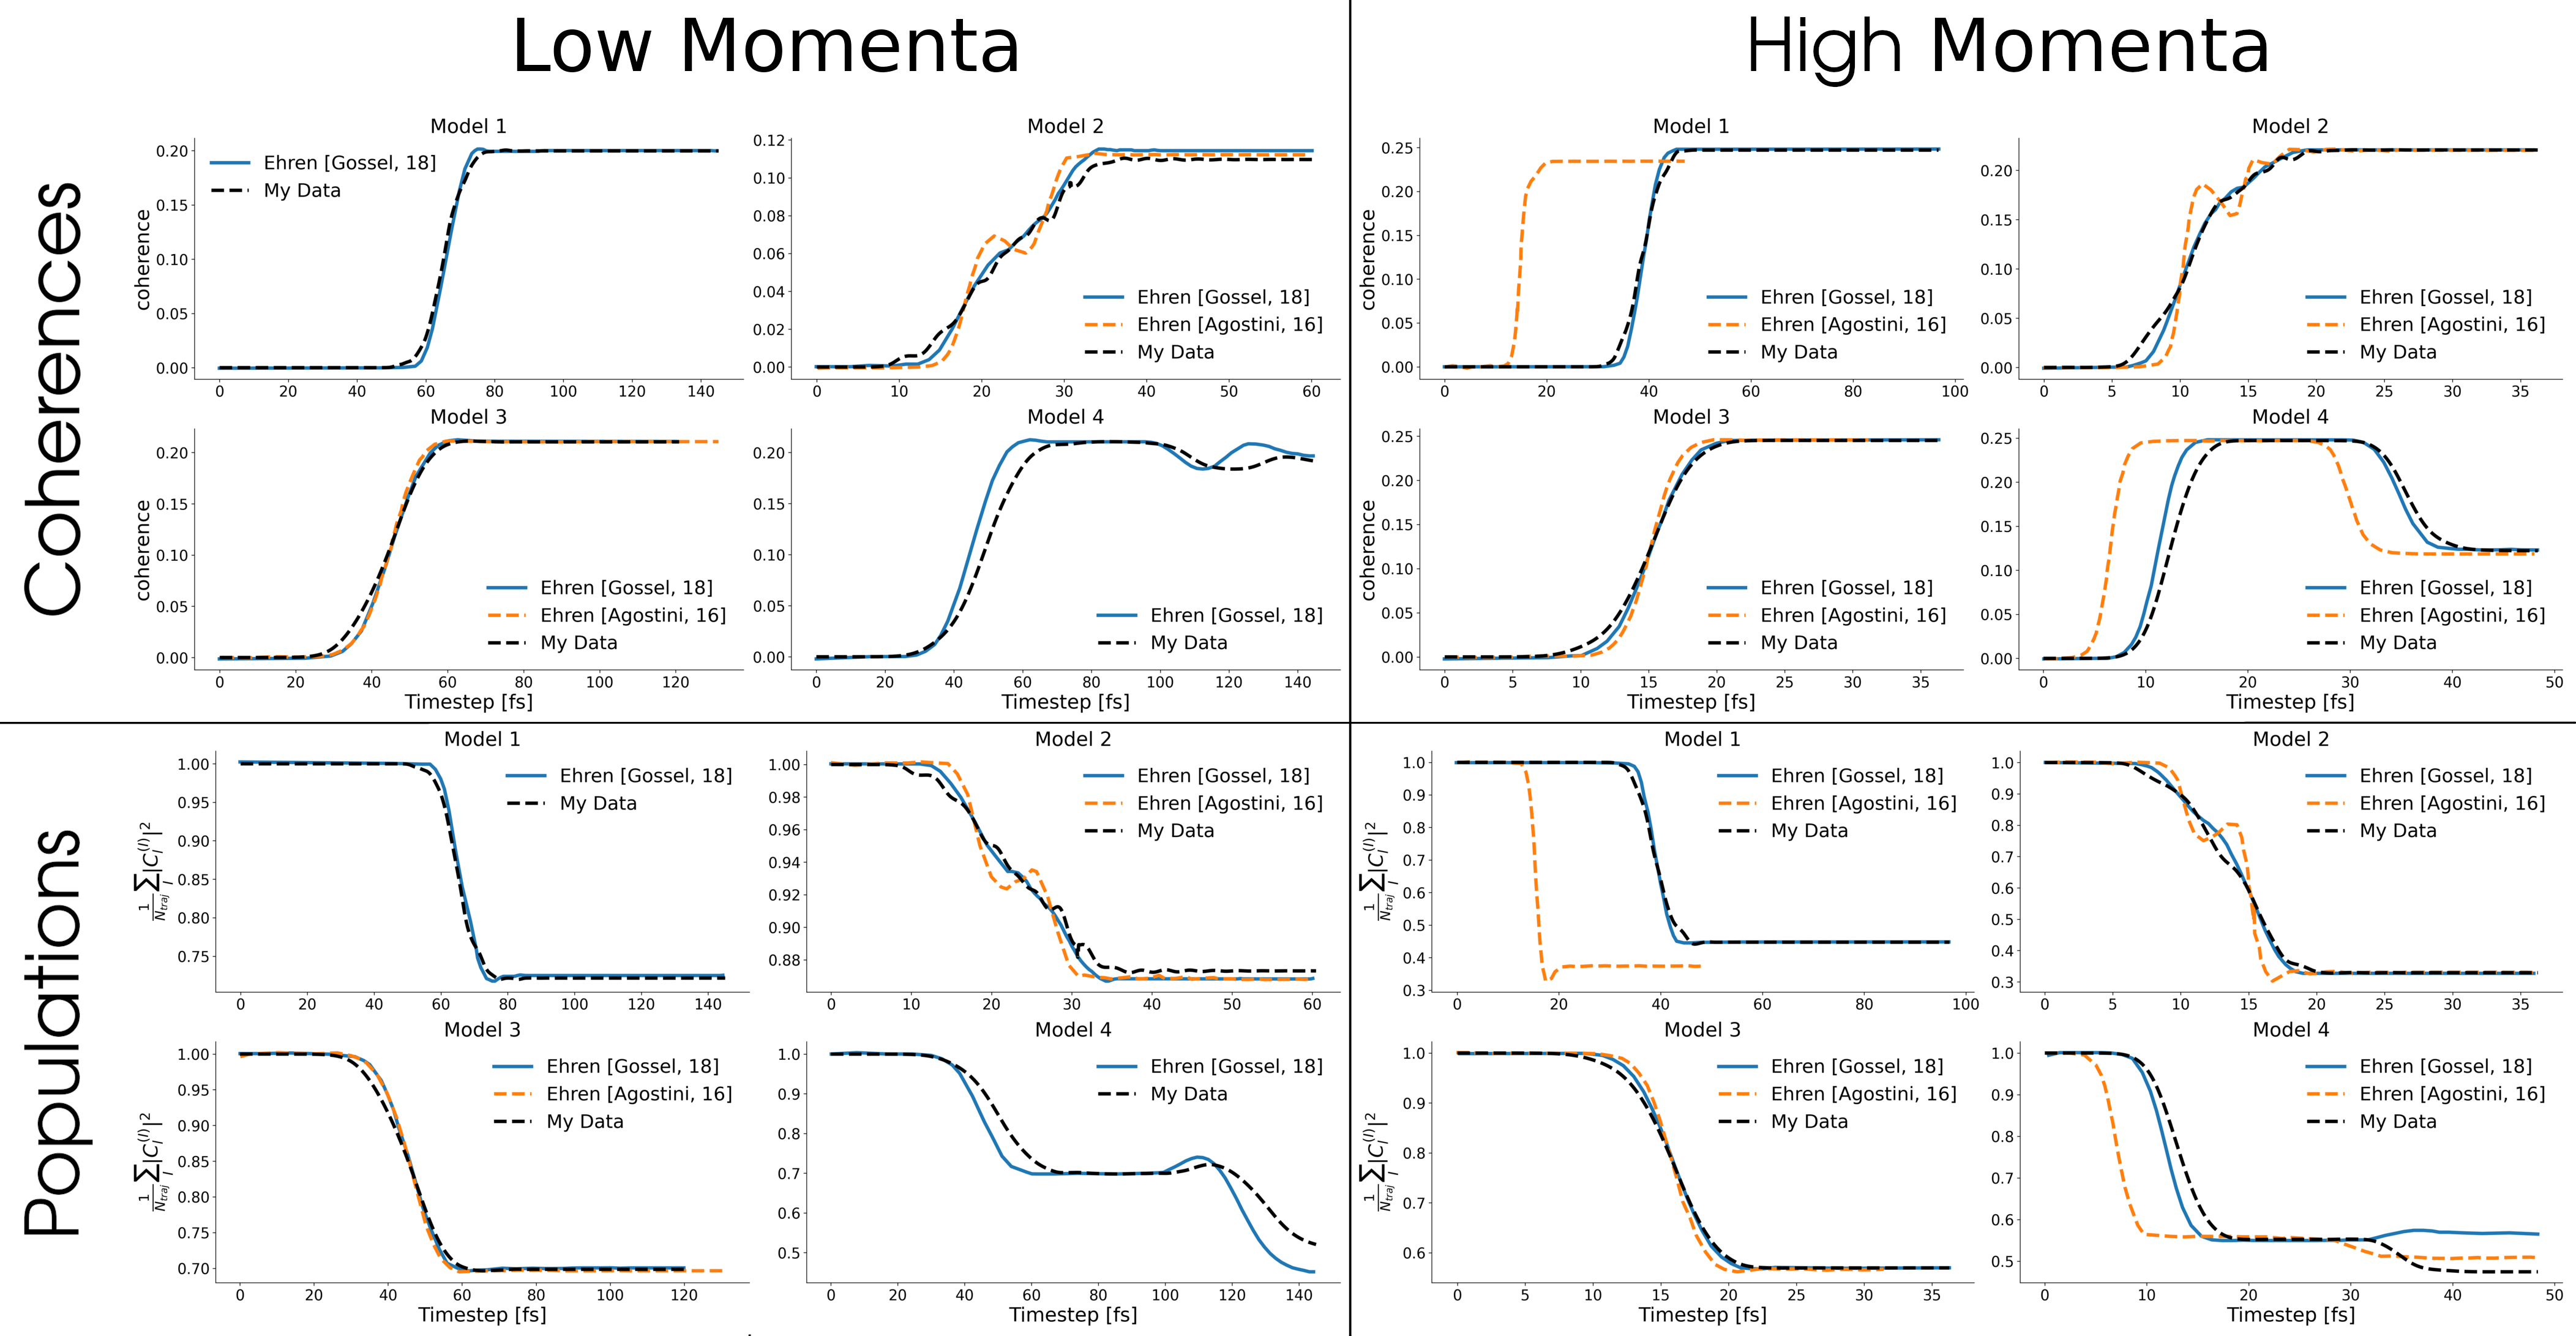
\includegraphics[width=\textwidth]{img/CTMQC/TullyModels/Ehren_LitComp.png}
	\caption{\label{fig:LitCompEhrenTully}A comparison of my implementation of Ehrenfest (for 4 model Hamiltonians) and results from the literature. The black dashed lines show my data (ground state ad pops), the orange dashed lines are data from Agostini, 16 \cite{agostini_quantum-classical_2016} and the blue solid lines are from Gossel, 18 \cite{gossel_coupled-trajectory_2018}. The figures are labelled with their model number, whether the initial momentum was high or low and whether the populations or coherence indicator was plotted.}
\end{figure}
\noindent My results as well as the relevant data taken from Agostini, 16 and Gossel, 18 \cite{agostini_quantum-classical_2016, gossel_coupled-trajectory_2018} are shown in figure \ref{fig:LitCompEhrenTully} for Ehrenfest dynamics. This is equivalent to full CTMQC dynamics where the quantum momentum term is set to 0. Hence, we can test most parts of the code (i.e. Runge-Kutta propagation, velocity verlet, inputs, force calculations etc...) while ignoring the new quantum momentum and accumulated adiabatic force terms.
\\\\
The results in figure \ref{fig:LitCompEhrenTully} show that both the adiabatic populations and coherence indicator give exactly the same results as in the literature, within reasonable error. Any deviations of results come from either a slightly different initial sampling of positions or small errors in extracting data from the graphs in each of the papers. For example, in the case of the high initial momentum simulation of model 4 all 3 results show some differences though the trend is very similar. This is true also in the Model 2 results where the Agostini, 16 populations show some transient oscillations before settling onto the same equilibrium population. This may be due to a smaller spread of positions being used in the initial sample leading to similar oscillations that aren't smoothed out in the averaging over all replicas. There are also a couple of models that start at a slightly different initial mean position in Frederica, 16 thus they hit the nonadiabatic crossing region sooner. These are model 1 and 4 for the high momentum case.
\\\\
Although not all results are exactly the same, I believe the populations agree well enough within a reasonable error to serve as a confirmation of my implementation.
\subsubsection{Subotnik, 2010}
As a final confirmation of my implementation, in a Subotnik, 2010 \cite{SubotnikMomentumEhrenfest}, results were published for Ehrenfest simulations carried out on the 3 original Tully Models. In this work, the author presented the probabilities of the population being found transmitted through the region of nonadiabatic coupling on the ground or excited state and the probability of being reflected on the ground or upper state. In the results below, I will show comparisons of just the transmission probability onto the ground state. That is, the population that travels on the ground state beyond the region of high nonadiabatic coupling. Other probabilities will not be shown in the interest of brevity, though they agree with the published results as well as the ground state transmission in figure \ref{fig:SubotnikComparison}.
\begin{figure}[ht]
  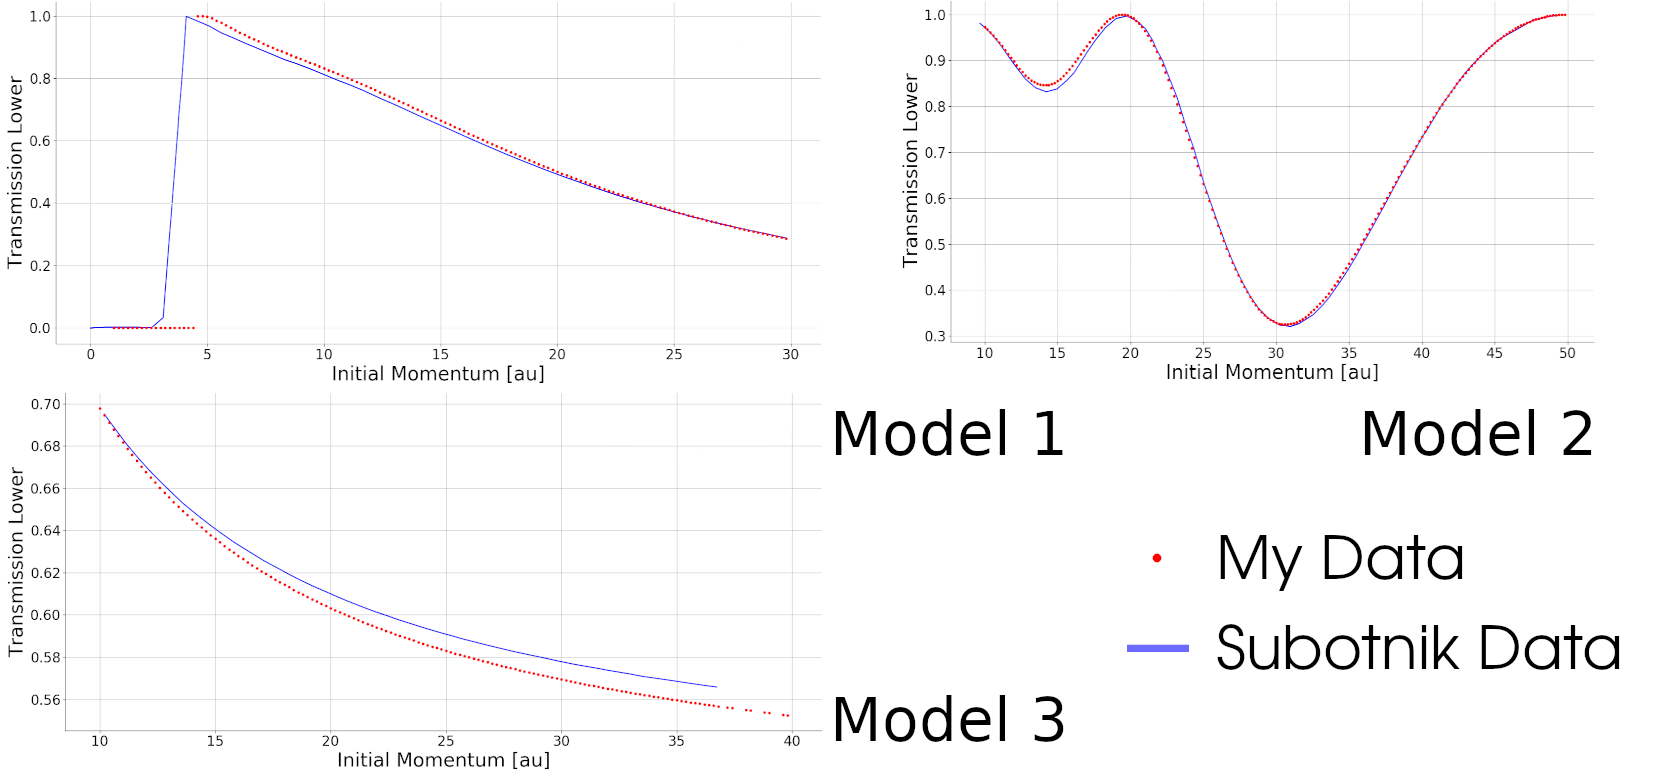
\includegraphics[width=\textwidth]{img/CTMQC/TullyModels/Ehrenfest_vs_Subotnik.png}
  \caption{\label{fig:SubotnikComparison}Comparison of transmission probabilities through the region of high nonadiabatic coupling on the ground state. Tully model 1 is shown in the top-left, Tully model 2 is shown in the top-right and Tully model 3 is shown in the bottom-left.}
\end{figure}
As can  be seen in figure \ref{fig:SubotnikComparison} my implementation of the Ehrenfest simulation code for the Tully models agrees very well with those in Subotnik, 2010 \cite{SubotnikMomentumEhrenfest}. The small deviation (less than 1\% maximum disagreement) within each model is due to errors in retrieving data from images in original paper and possibly slightly different analysis methods.
\\\\
These tests serve as a confirmation of the implementation of the Ehrenfest propagator. The full CTMQC equations can be implemented using the majority of the Ehrenfest infrastructure with extensions to account for the quantum momentum terms.

\section{Testing my implementation -CTMQC}
\subsection{Conservation of the norm}
In figure \ref{fig:CTMQCNormCons} only Model 3 shows a similar trend as in Ehrenfest for the norm conservation -i.e. a decreasing electronic timestep gives a rapidly decreasing norm drift. In models 1 and 2 we see that the norm drift doesn't get much better as we decrease the timestep and there are large error bars associated with each data point. In model 4 this is less pronounced but is still clearly affected. This is due to an instability in the current formalism of the quantum momentum term ($\mathcal{Q}_{lk, \nu}^{(I)}$).
\begin{figure}[ht]
	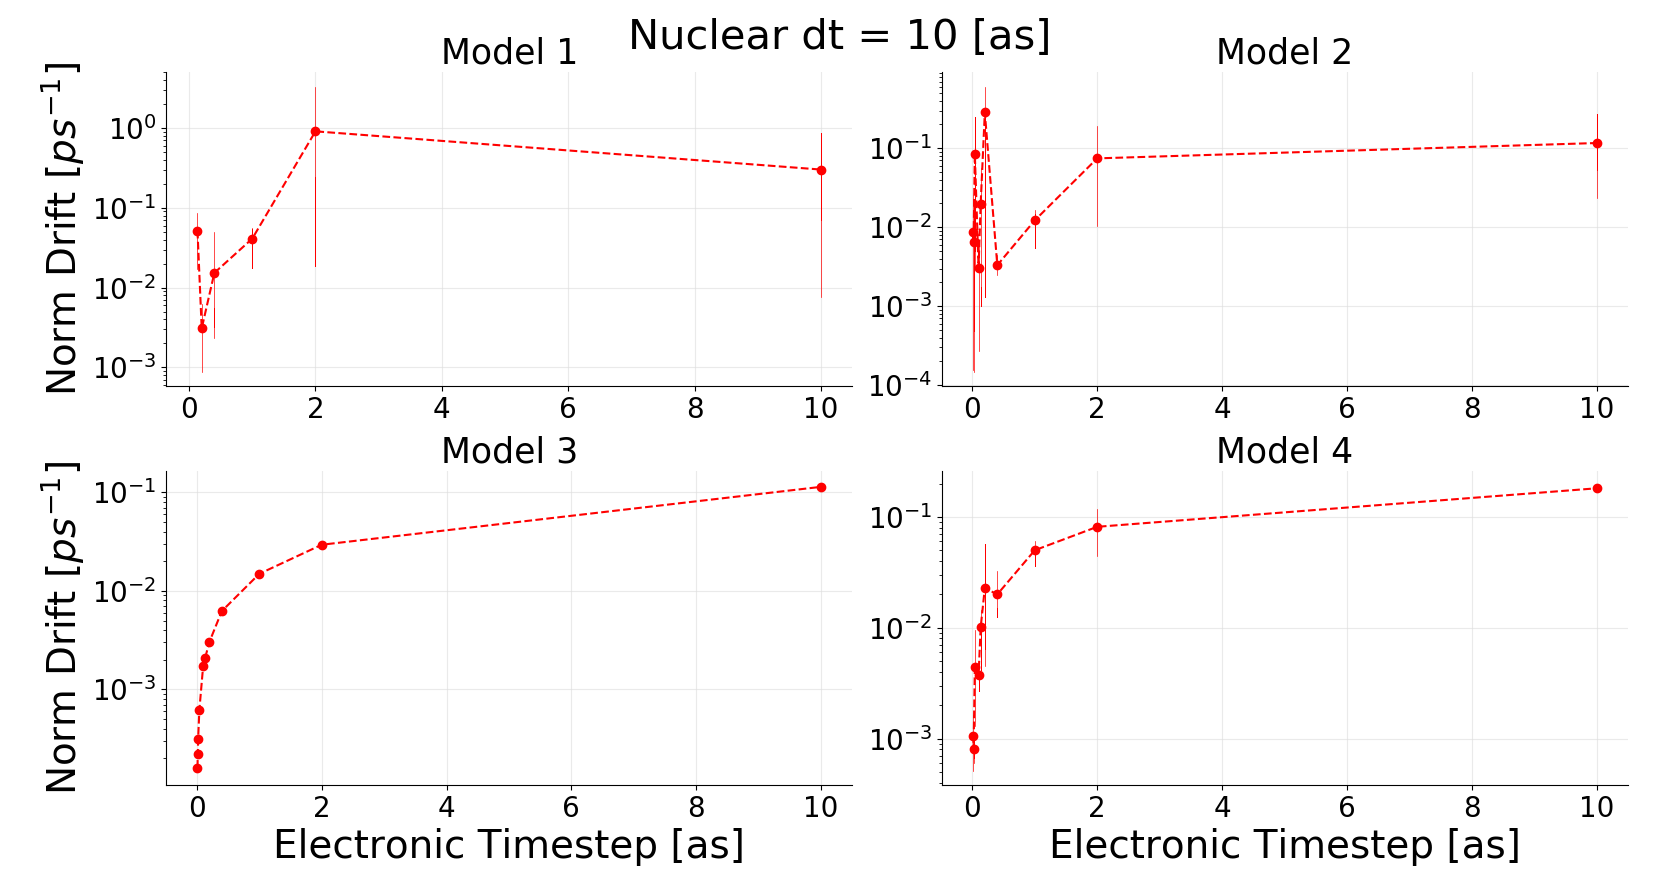
\includegraphics[width=\textwidth]{/home/matt/Documents/PhD/PhD_Thesis/img/CTMQC/TullyModels/CTMQC_Norm_Conservation.png}
	\caption{\label{fig:CTMQCNormCons}The norm conservation when using standard CTMQC as outlined in the literature for each of the Tully models. These simulations were ran with a high initial momentum. The red markers show data points and vertical bars show error bars associated with each point.}
\end{figure}
\\\\
The calculation of the quantum momentum is discussed in detail in Min, 17 \cite{min_ab_2017} and outlined in the introduction to the thesis in section \ref{sect:QM_Calc}. As mentioned in that section, the denominator in the expression for $\mathbf{R}_{lk, \nu}$ may be positive or negative and when it switches between each it can approach zero very closely. If this denominator approaches zero more quickly that the numerator then we can see large divergence in the $\mathbf{R}_{lk, \nu}$ term which can lead to large norm drifts. This is highlighted in figure \ref{fig:QlkSpike}.

\subsubsection{Quantum Momentum Instabilities}
\label{sect:QlkSpikes}
\begin{figure}[ht]
	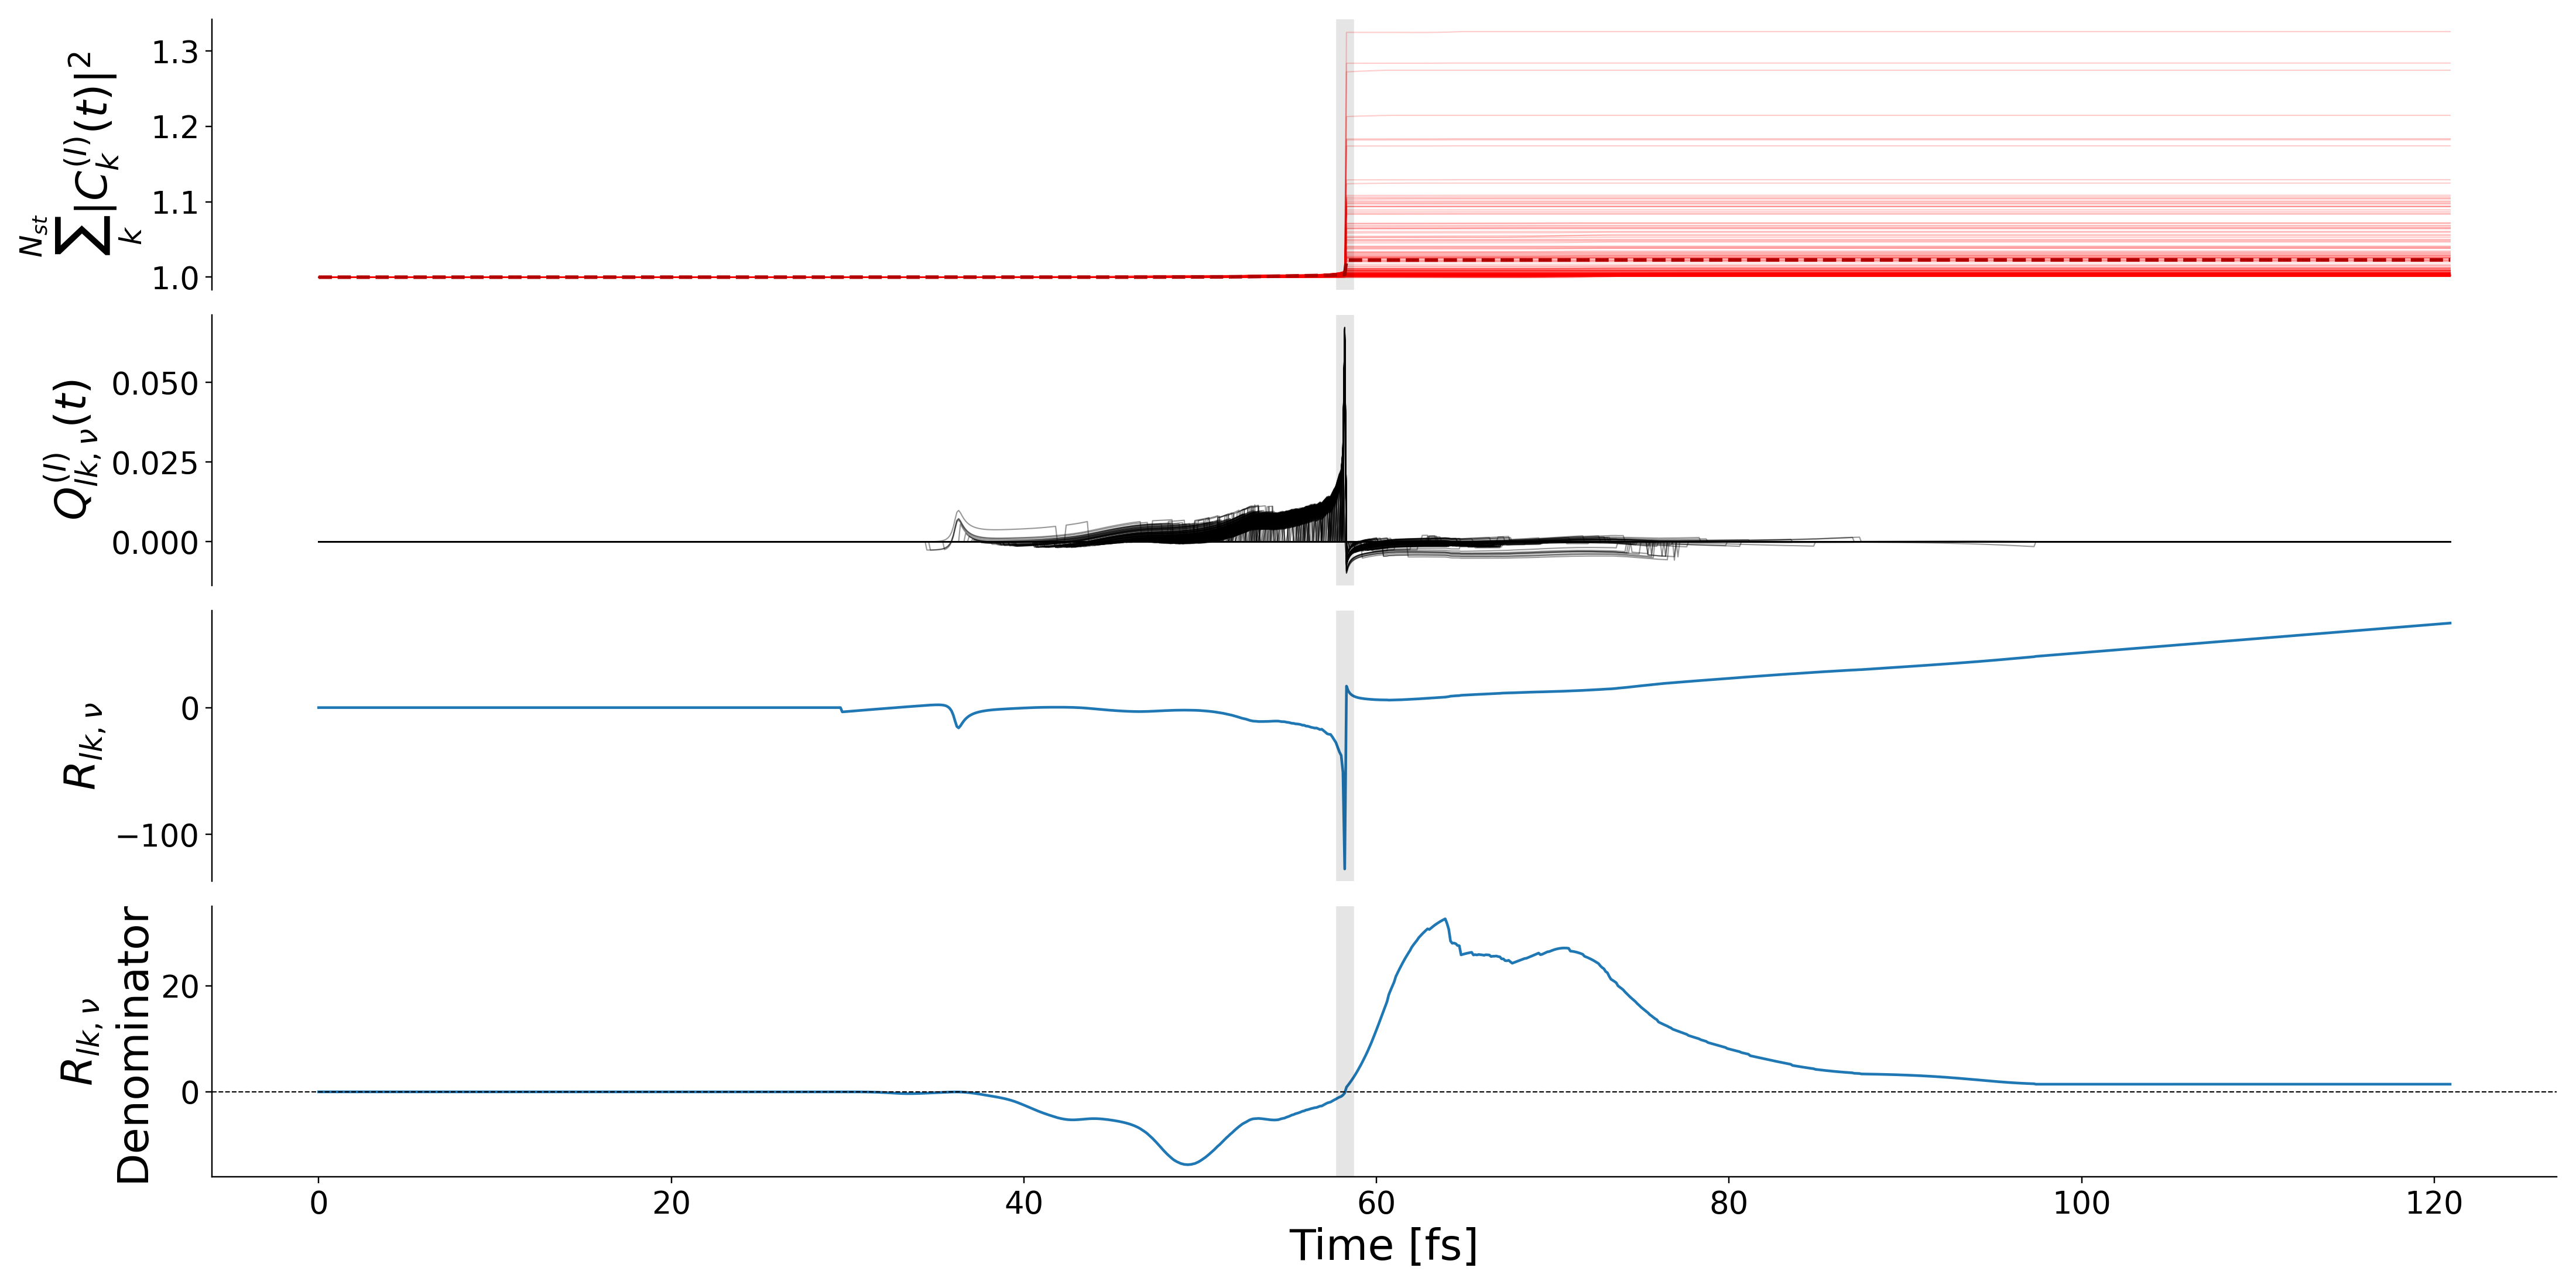
\includegraphics[width=\textwidth]{./img/CTMQC/TullyModels/Spikes/RlkDenom_Rlk_Qlk_Norm.png}
	\caption{\label{fig:QlkSpike}As the denominator of the $\mathbf{R}_{lk,\nu}$ term approaches zero (bottom panel) the full $\mathbf{R}_{lk, \nu}$ term (2$^{\text{nd}}$ to bottom panel) can approach infinity which propagates through the $\mathcal{Q}_{lk, \nu}^{(I)}$ term (2$^{\text{nd}}$ to top panel) causing discontinuities and norm drift in the populations (top panel). The grey vertical bar denotes the region the denominator approaches 0. The thin solid red lines in the top panel show the norm drift for individual replicas.}
\end{figure}
\noindent In figure \ref{fig:QlkSpike}, as the denominator of quantum momentum intercept (the bottom panel) approaches 0 the $\mathbf{R}_{lk, \nu}$ term may spike causing a discontinuity in the populations (through the quantum momentum). The reason this only occurs in Models 1, 2 and 4 is due to the fact that the difference in the adiabatic momenta terms ($\mathbf{f}_{l, \nu}^{(I)} - \mathbf{f}_{k, \nu}^{(I)}$) doesn't cross 0 in Model 3 as the time-derivative of the adiabatic energies is always either positive or negative. 
\\\\
In order to correct for this divergence I have investigated a number of alterations to the calculation of the quantum momentum. These depend on the detection of the spikes/divergences in the $\mathbf{R}_{lk, \nu}$ term and then the appropriate treatment of them. A divergence is recorded is 2 conditions are met. First is a simple threshold on the time-derivative of the intercept term, i.e. $|\frac{\delta}{\delta t} \mathbf{R}_{lk, \nu}| > thresh$. The second condition is a threshold on the intercept denominator i.e. $|\mathbf{R}denom_{lk, \nu}| < thresh$. For example, if the absolute time-derivative of the $\mathbf{R}{lk, \nu}$ term is larger than a value (say 5) and the bottom of the fraction in equation \eqref{eq:Rlk} is within 0.01 of 0 then we assume the $\mathbf{R}_{lk, \nu}$ term is diverging and the simulation code then uses a different method of propagating the electronic coefficients.
\noindent The alternative propagation methods that have been investigated are:
\begin{enumerate}
	\item Use Ehrenfest Dynamics (set e.g. $\mathcal{Q}_{lk, \nu}$ term to 0).
	\item Extrapolate the value of $\mathbf{R}_{lk, \nu}$ from values before the divergence (see appendix \ref{ap:RlkExtrap}).
	\item Switch to using the alternative intercept $\mathbf{R}_{0, \nu}^{(I)}$ (see appendix \ref{ap:AltIntercept}).
\end{enumerate}
of these 3 methods, method 3 was the most successful in reducing the norm drift in the Tully Models as can be seen in figure \ref{fig:NormConsCorr}.
\begin{figure}[ht]
	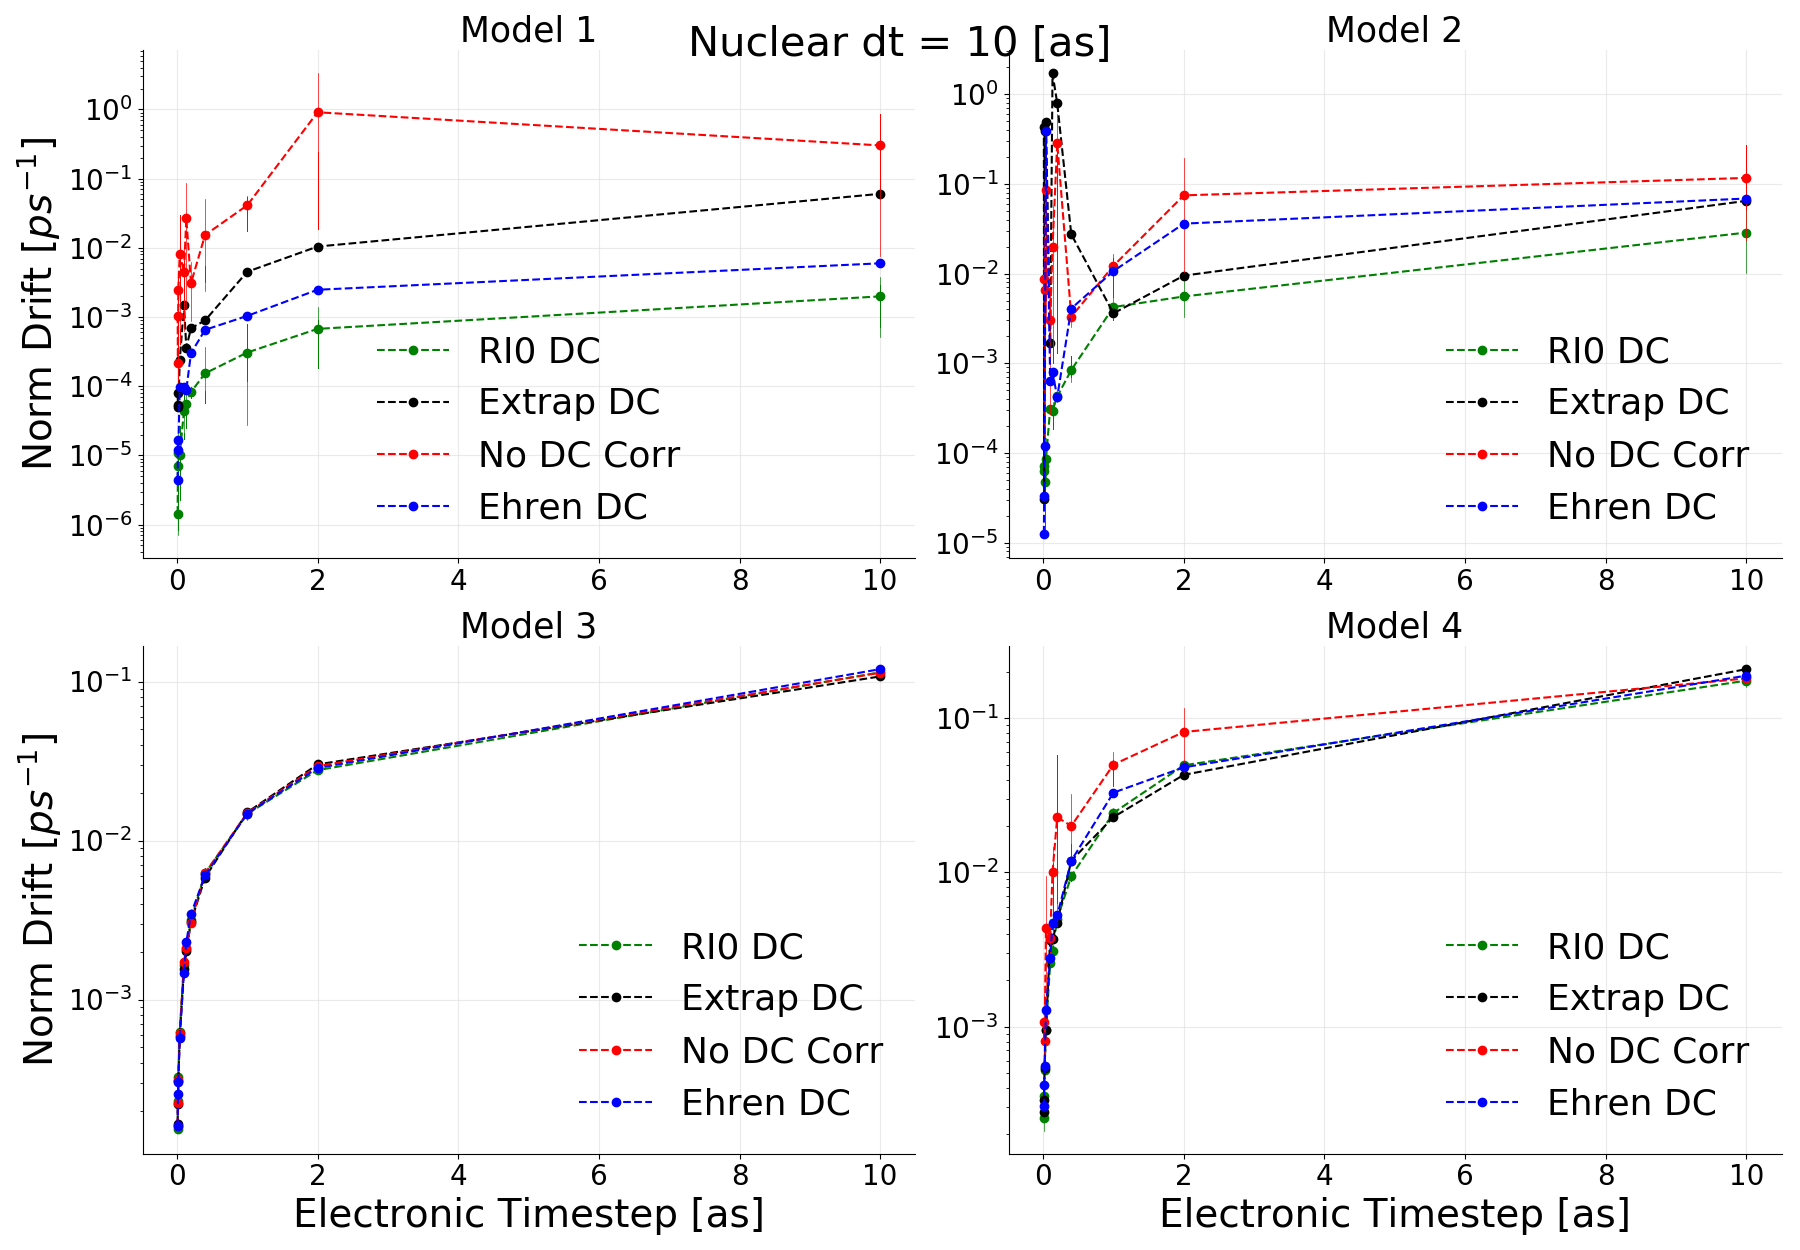
\includegraphics[width=\textwidth]{img/CTMQC/TullyModels/CTMQC_Norm_Conservation_wCorr.png}
	\caption{\label{fig:NormConsCorr}Norm conservation in CTMQC after applying a divergence correction to the $\mathbf{R}_{lk, \nu}$ term. RI0 refers to method 3, Extrap DC refers to method 2 and Ehren DC refers to method 1. No DC Corr shows the population norm without any corrections applied.}
\end{figure}
\\
In figure \ref{fig:NormConsCorr} we see the norm drift results after the 3 $\mathbf{R}_{lk, \nu}$ correction methods have been applied. The red curve shows the original data (as in figure \ref{fig:CTMQCNormCons}) with it's large divergences in the norm drift. The green curve shows the alternative intercept method, the blue curve shows the effect of switching to Ehrenfest during the $\mathcal{Q}_{lk, \nu}^{(I)}$ spikes and the black shows a method that involved extrapolating the $\mathbf{R}_{lk, \nu}$ value from data before the spike began. We can see clearly all 3 methods improve the norm drift, though using the alternative intercept seems to help the most. Model 3 is not affected as we do not see these divergences in the $\mathbf{R}_{lk, \nu}$ due to the denominator in this particular model never crossing from positive to negative (through zero). It is important to note that in each of the models with the divergence correction applied all models exhibit the expected trend of decreasing the time-step improves norm conservation. However, the norm conservation in all 4 models is still significantly higher ($\sim$ 7-8 orders of magnitude) higher than that of Ehrenfest. I think this is due to the product of the adiabatic populations, $|C_{l}^{(I)}|^2 |C_{k}^{(I)}|^2$, being used in the calculation of the quantum momentum which can be a more quickly varying quantity than just the adiabatic populations alone.

\subsection{Mathematical Tests}
Multiple tests of the implementation of the quantities in the equations have been implemented in the code to ensure correct outputs. A checklist of any mathematical tests is given below:
\begin{itemize}
  \item Checking the (anti-)symmetry of the (NACV) Hamiltonian when constructed
  
  \item Comparing the adiabatic momentum term to post-production time-integrated adiabatic energies (using trapezium rule)
  
  \item Checking special case solutions when all replicas are initialised at the same position such as:
	\begin{itemize}
	  \item $\mathcal{Q}_{lk, \nu}^{(I)} = 0$
	  \item CTMQC = Ehrenfest
	\end{itemize}

  \item Checking special cases for when $\sigma$ is replica independent (i.e. $\sigma^{(I)} = \sigma$):
	\begin{itemize}
	  \item $\sigma = \frac{\hbar}{2 \sigma^2}$
	  \item $\mathbf{R}_{lk, \nu} = \mathbf{R}_{\nu}^{(I)} \frac{\hbar}{2 \sigma^2}$ (Assuming the positions, $\mathbf{R}_{\nu}^{(I)}$ are also replica independent)
	\end{itemize}

  \item If all adiabatic population is localised on a single state ($|C_{l}^{(I)}|^2 = [1, 0, 0, \cdots, 0]$). Then we get Ehrenfest dynamics on that replica.
  \item Solving the static Schr\"odinger equation gives Rabi oscillation \cite{FeynmanLectVol3}. See appendix \ref{ap:Rabi}.
\end{itemize}

I have also provided 2 (more substantial) mathematical tests for the code below in the following sections.
\subsubsection{Time Derivative of Replica-Sum of Adiabatic Populations}
\begin{figure}[ht]
	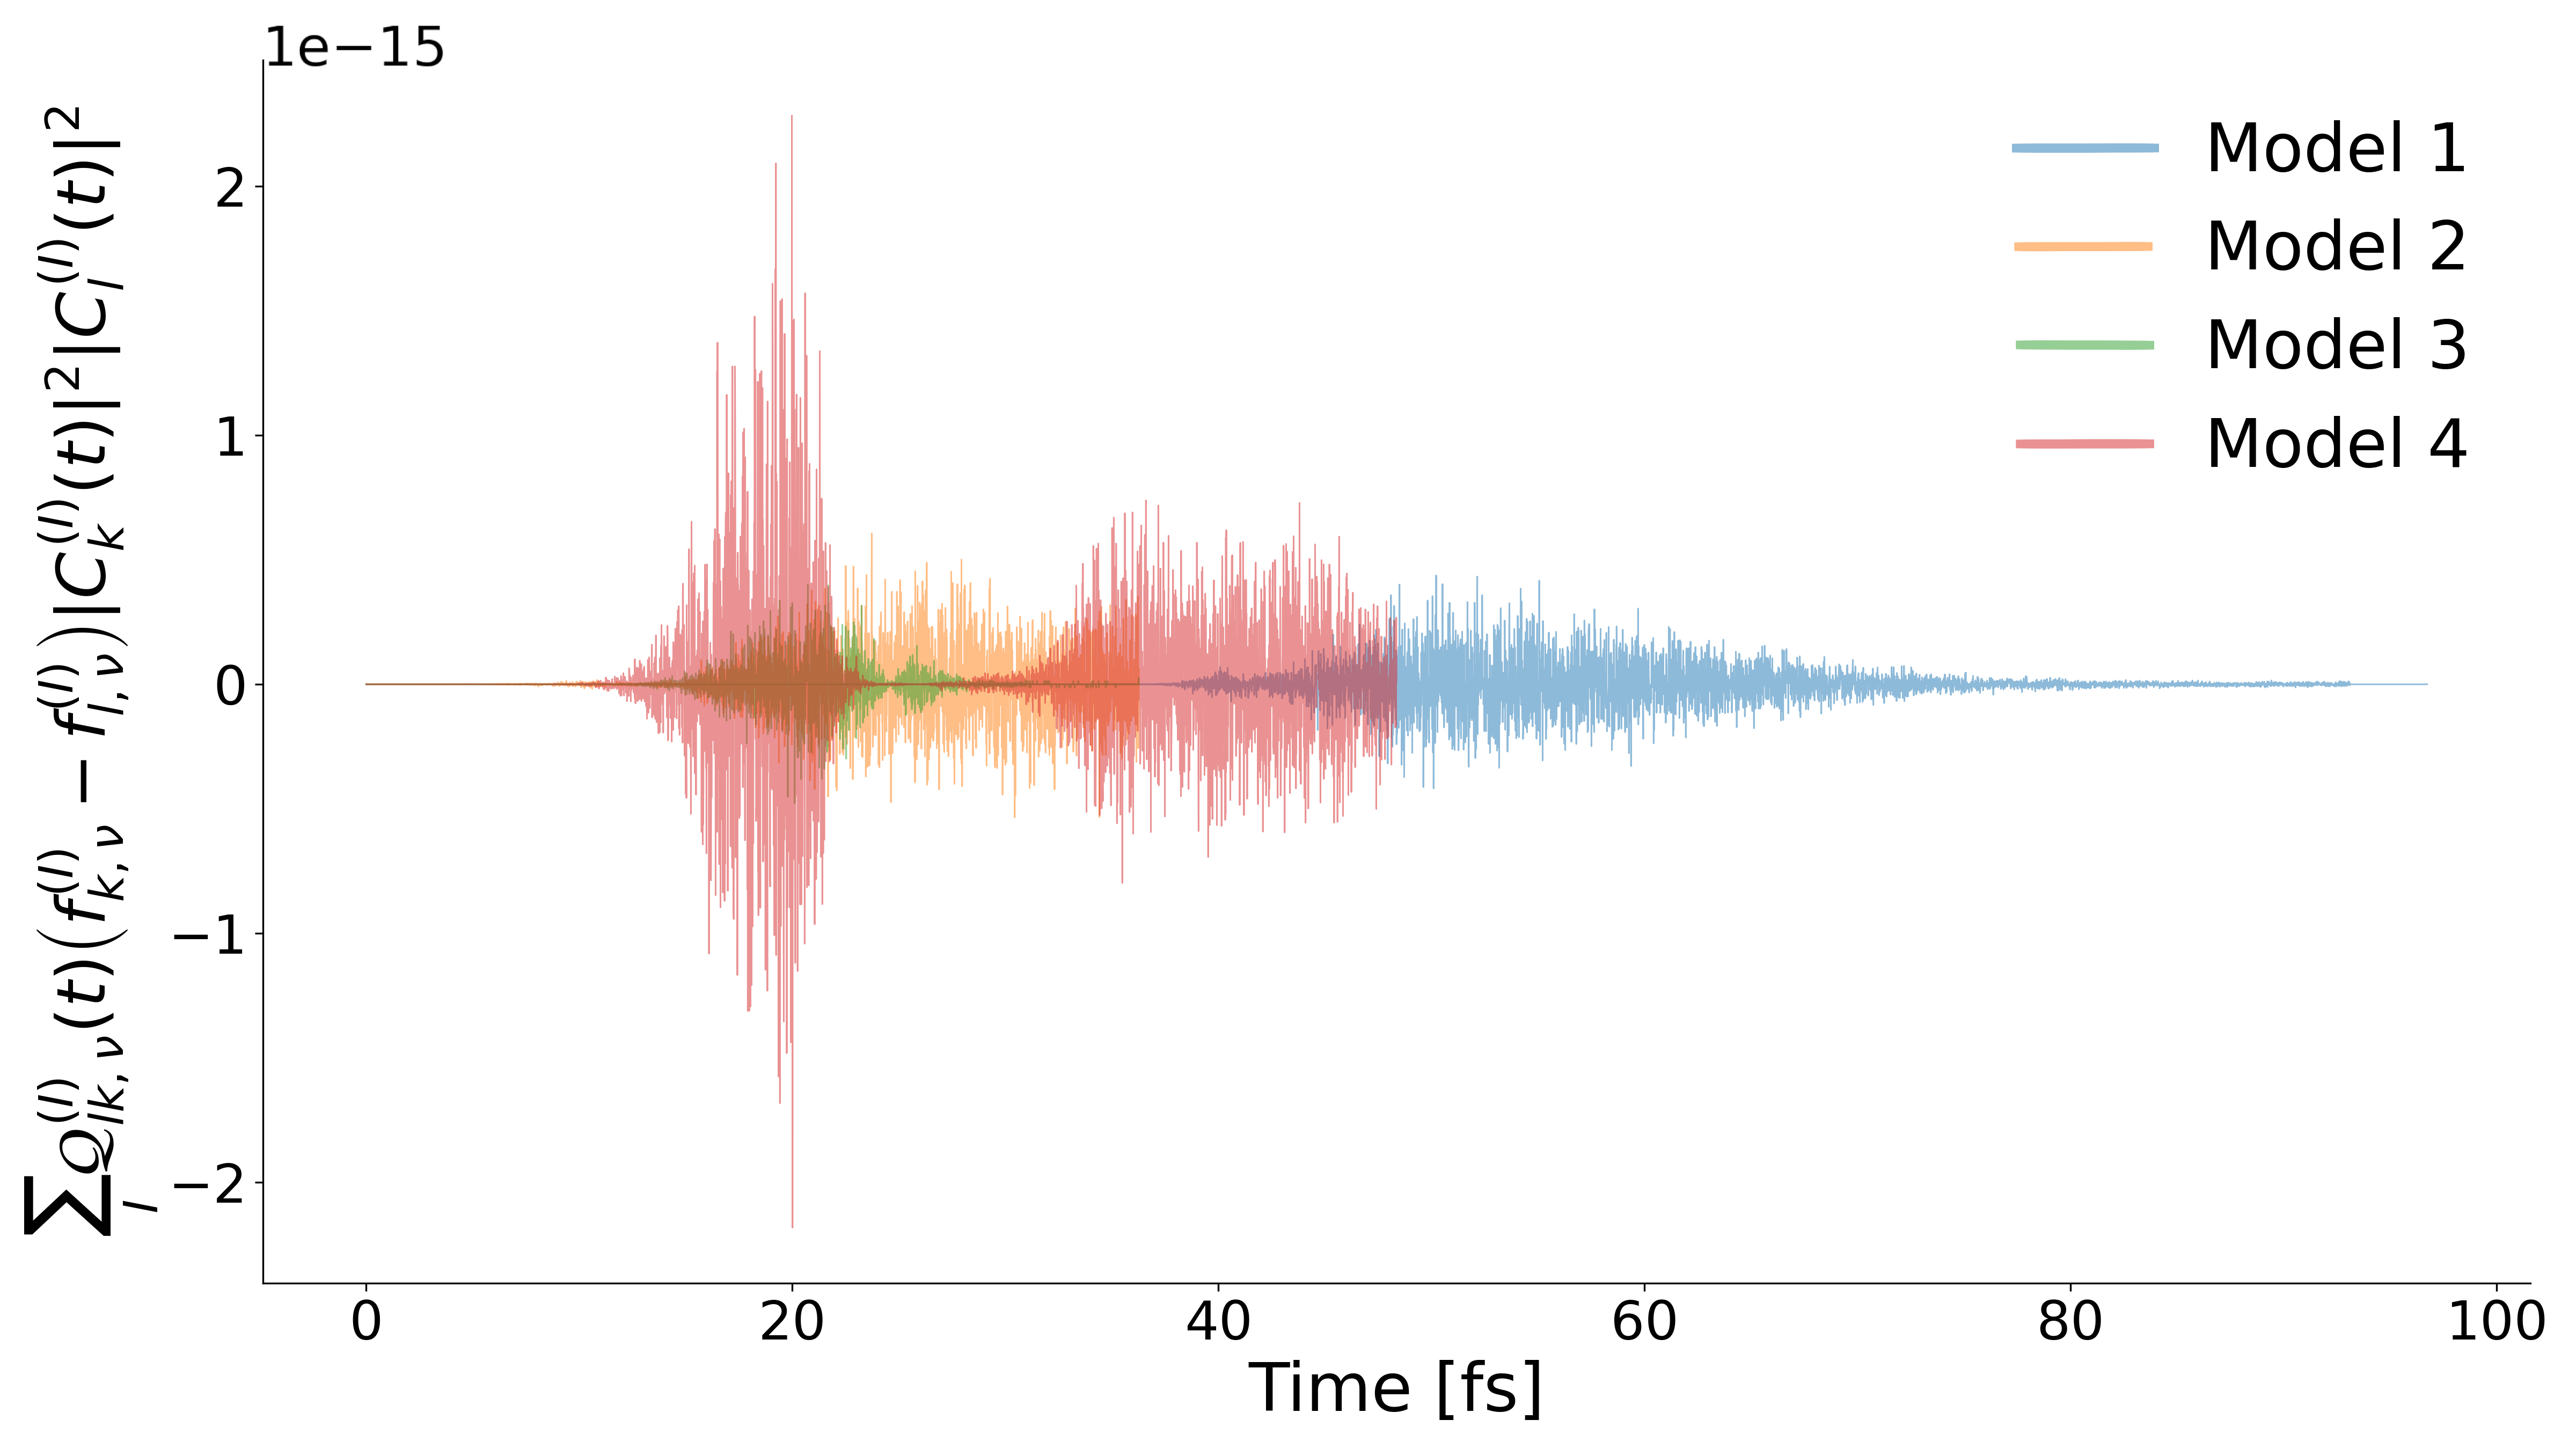
\includegraphics[width=\textwidth]{./img/CTMQC/TullyModels/CTMQC_S27.png}
	\caption{\label{fig:S27}The conserved quantity given in equation \eqref{eq:S27}. Each color represents data outputted by a simulation using a different model (specified in the legend). Each time-series is plotted with a translucent color meaning each model's data can be seen at once.}
\end{figure}

In the SI of Min, 17 \cite{min_ab_2017} a conservation equation (S27) is given. This is repeated below in equation \eqref{eq:S27}
\begin{equation}
	\sum_{I} \mathcal{Q}_{lk, \nu}^{(I)}(t) \left( f_{k, \nu}^{(I)} - f_{l, \nu}^{(I)} \right) |C_{k}^{(I)} (t)|^2 |C_{l}^{(I)} (t)|^2 = 0  \qquad \forall l, k, \nu
	\label{eq:S27}
\end{equation}

An example time-series of this quantity is given in figure \ref{fig:S27} for each Tully model. The data used to calculate come from simulations of each of the Tully models using the parameters given in appendix \ref{ap:tully_params}. No smoothing was used for the $\mathbf{R}_{lk, \nu}^{(I)}$ term. It can be seen in this figure that the conservation quantity hovers around 0 for each model with a maximum deviation of 10$^{-15}$ m$_{e}$Ha.

\subsubsection{$\sum_{l} \mathbb{X}_{qm, ll} |C_{l}^{(I)}|^2$}
\label{sect:sumXqmll}
As the equations are currently formulated another numerical test validating the quantum momentum part of the propagation equations for the coefficients can be used. The CTMQC equation for the propagation of the adiabatic expansion coefficients is given in equation \eqref{eq:elec_adiab}. The quantum momentum part of this equation is given below in equation \eqref{eq:qmCTMQCAdiab}. 
\begin{equation}
  \mathbb{X}_{qm, ll}^{(I)} = \sum_{\nu=1}^{N_n}\sum_{k} \frac{\mathcal{Q}_{lk, \nu}^{(I)}}{\hbar     M_\nu} \cdot \left[ \mathbf{f}_{k,\nu}^{(I)} - \mathbf{f}_{l,\nu}^{(I)}   \right] |C_{k}^{(I)}|^2
  \label{eq:qmCTMQCAdiab}
\end{equation}
Where $\mathbb{X}_{qm, ll}^{(I)}$ is the diagonal matrix that, when multiplied with the adiabatic expansion coefficients, gives the quantum momentum contribution to the propagation of the expansion coefficients.I
\\\\
We can test the construction of this matrix within the code by multiplying by the adiabatic populations and summing as shown in equation \eqref{eq:NumericalTestXqmll}. It can be shown, assuming perfect norm conservation, that this should equal exactly 0 -due to the symmetry of the $|C_{l}^{(I)}|^2|C_{k}^{(I)}|^2$ and the quantum momentum matrix. This is checked for every timestep during propagation.

\begin{equation}
  \sum_{l} \mathbb{X}_{qm, ll}^{(I)} |C_{l}^{(I)}|^2 = 0
  \label{eq:NumericalTestXqmll}
\end{equation}


\subsection{Energy Conservation}
In Agostini, 16 \cite{agostini_quantum-classical_2016} it is stated that the approximate potential energy is given by the same equation as in Ehrenfest, i.e. equation \eqref{eq:EhrenfestEnergyConservation} a population weighted average of the potential energy surfaces. The 4 high momentum Tully models were simulated with various nuclear timesteps and a straight line of best fit was fitted to the total energy term.
\begin{figure}[ht]
  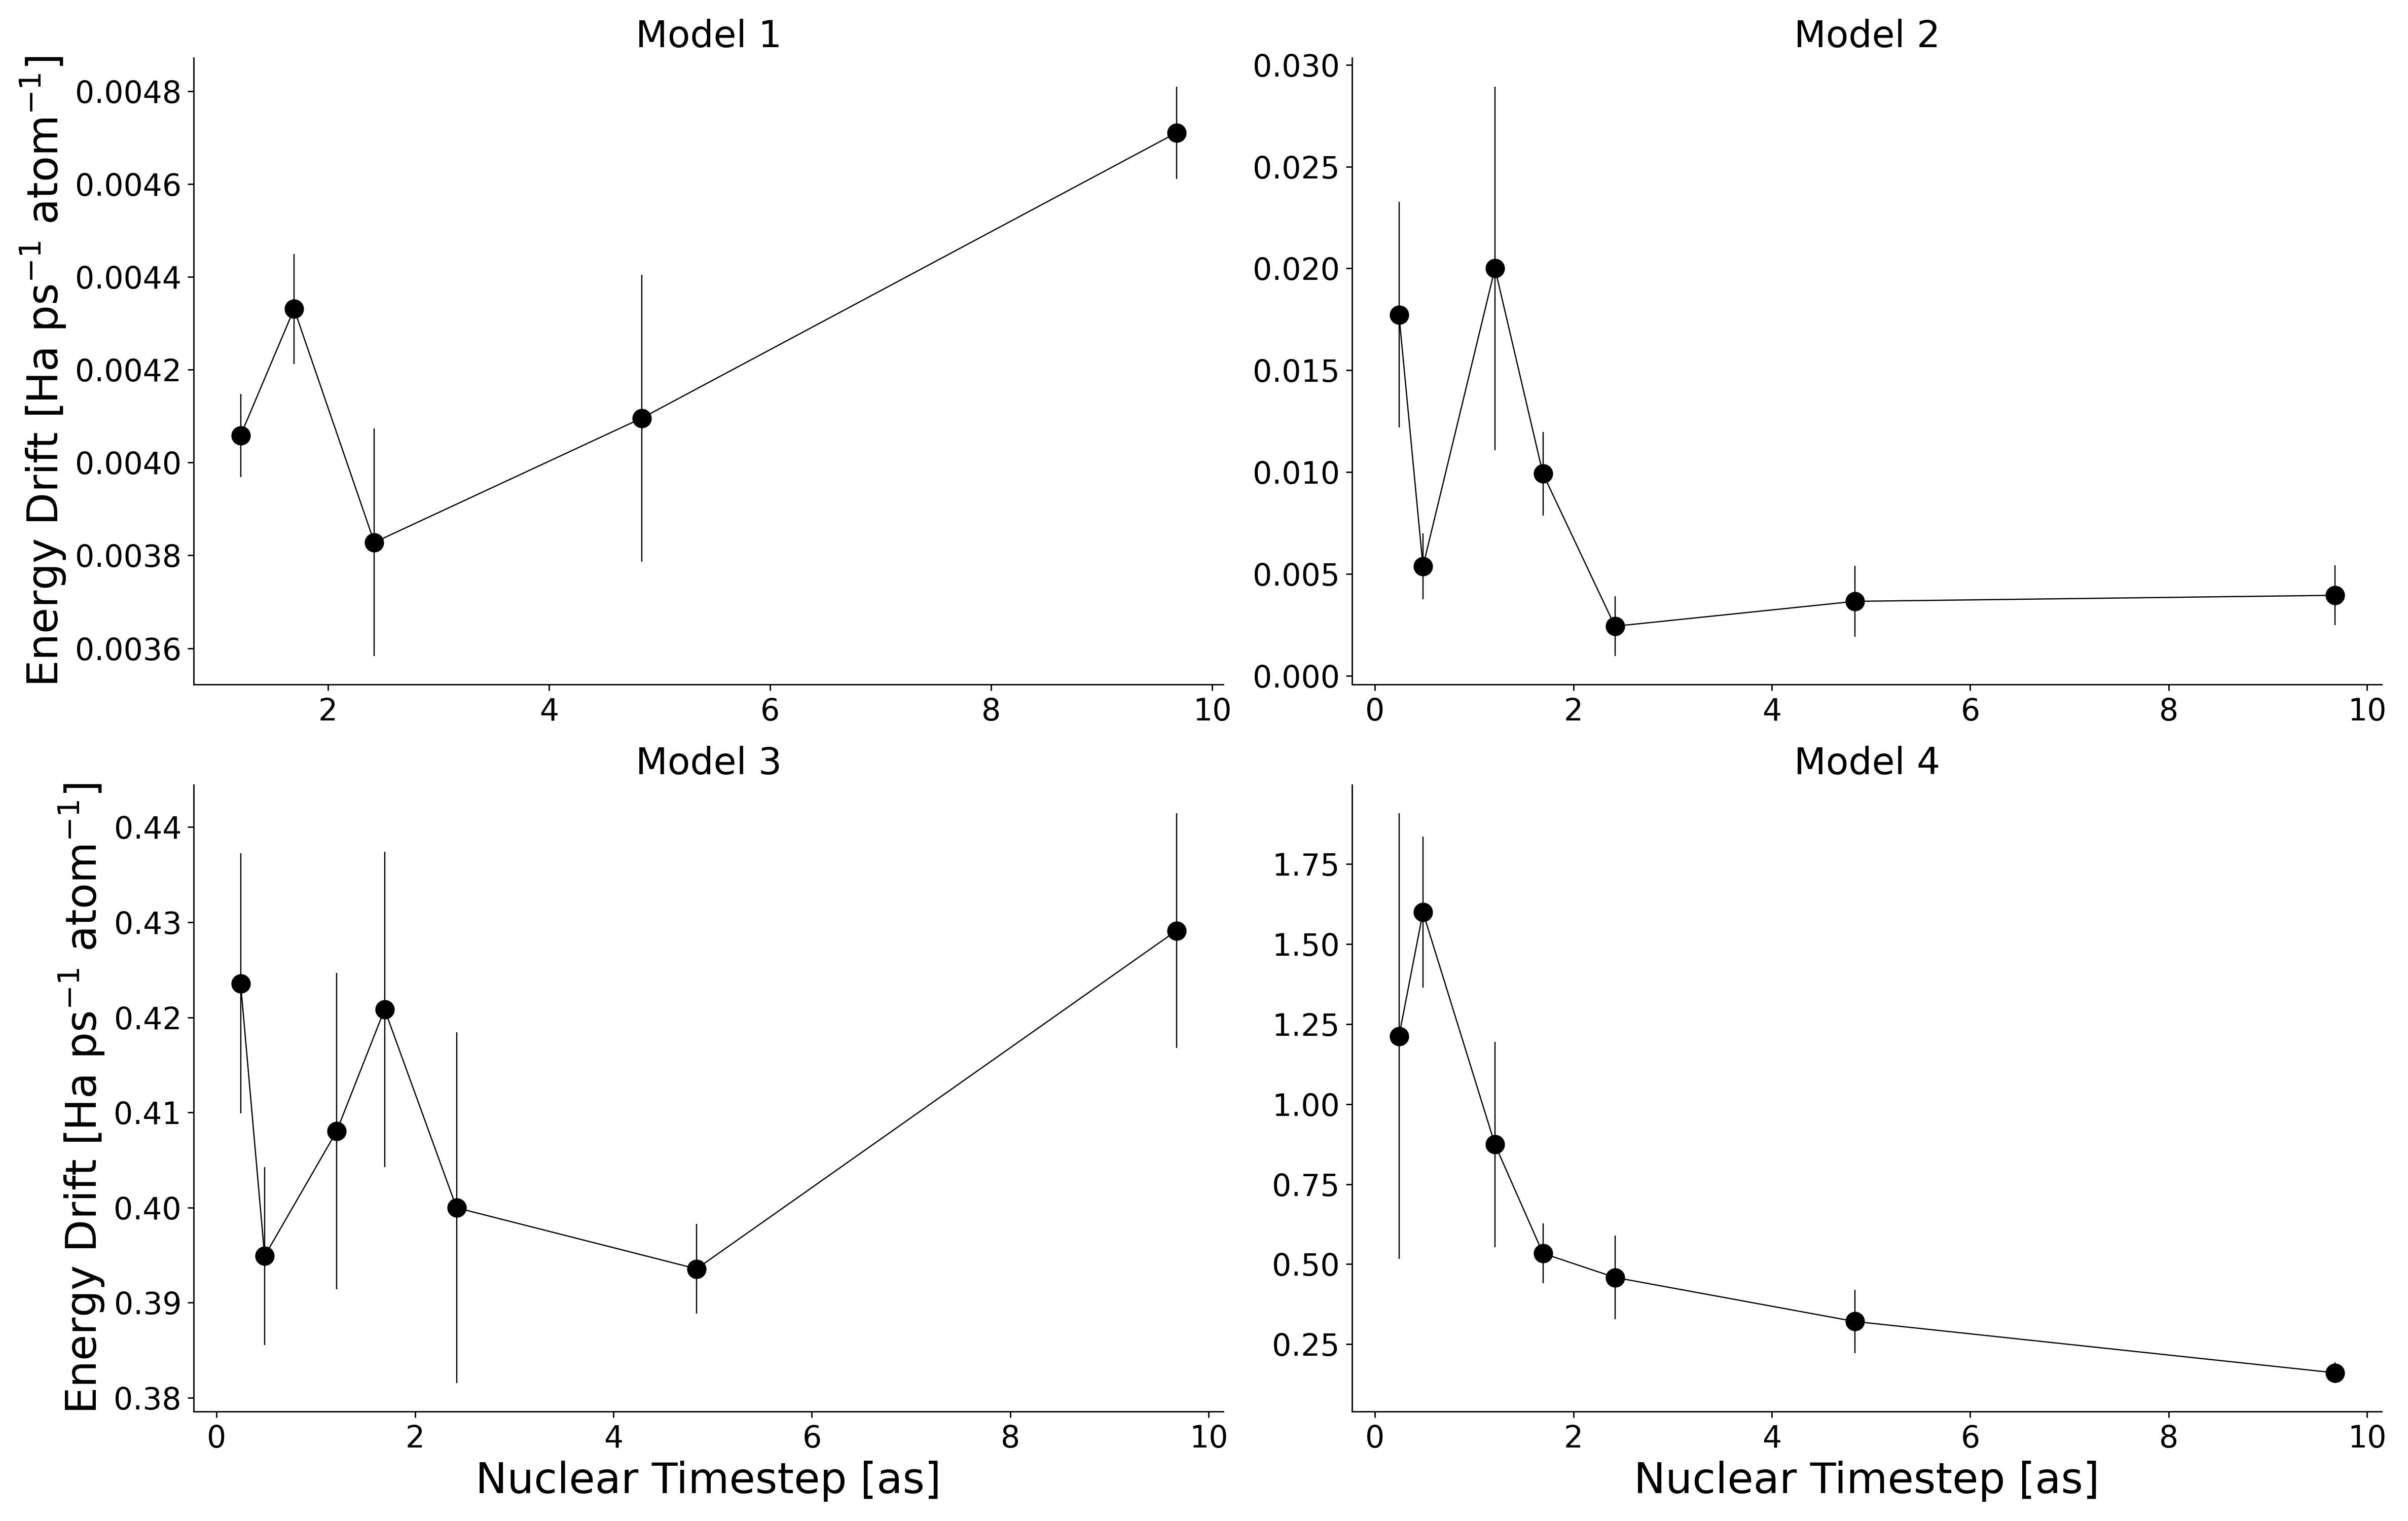
\includegraphics[width=\textwidth]{./img/CTMQC/TullyModels/CTMQC_EnerCons.png}
  \caption{\label{fig:CTMQC_EnergyCons}Energy drift in the 4 Tully models using the full CTMQC equations. Error bars are from multiple simulations carried out with different random sampling of the initial positions and momenta.}
\end{figure}
\\
As can be seen in figure \ref{fig:CTMQC_EnergyCons} the energy conservation in CTMQC does not improve with a decreasing nuclear timestep. In fact in the energy conservation worsens with decrease nuclear timestep in some models such as model 4. Additionally, in models 2 and 4 the errorbar increases as the timestep decreases. This is caused by an increased likelihood of coming across a divergence in the quantum momentum that can't be properly corrected, due to more steps being simulated. In model 3, the error bar stays the fairly consistent, and the energy conservation doesn't change with respect to the timestep. In this model there are no quantum momentum divergences which means the poor energy conservation is caused by something else. The potential energy as given in Agostini, 16 \cite{agostini_quantum-classical_2016} is an approximation and to achieve energy conservation comparable to Ehrenfest this may need amending.

\subsection{Comparisons to literature}
\begin{figure}[ht]
	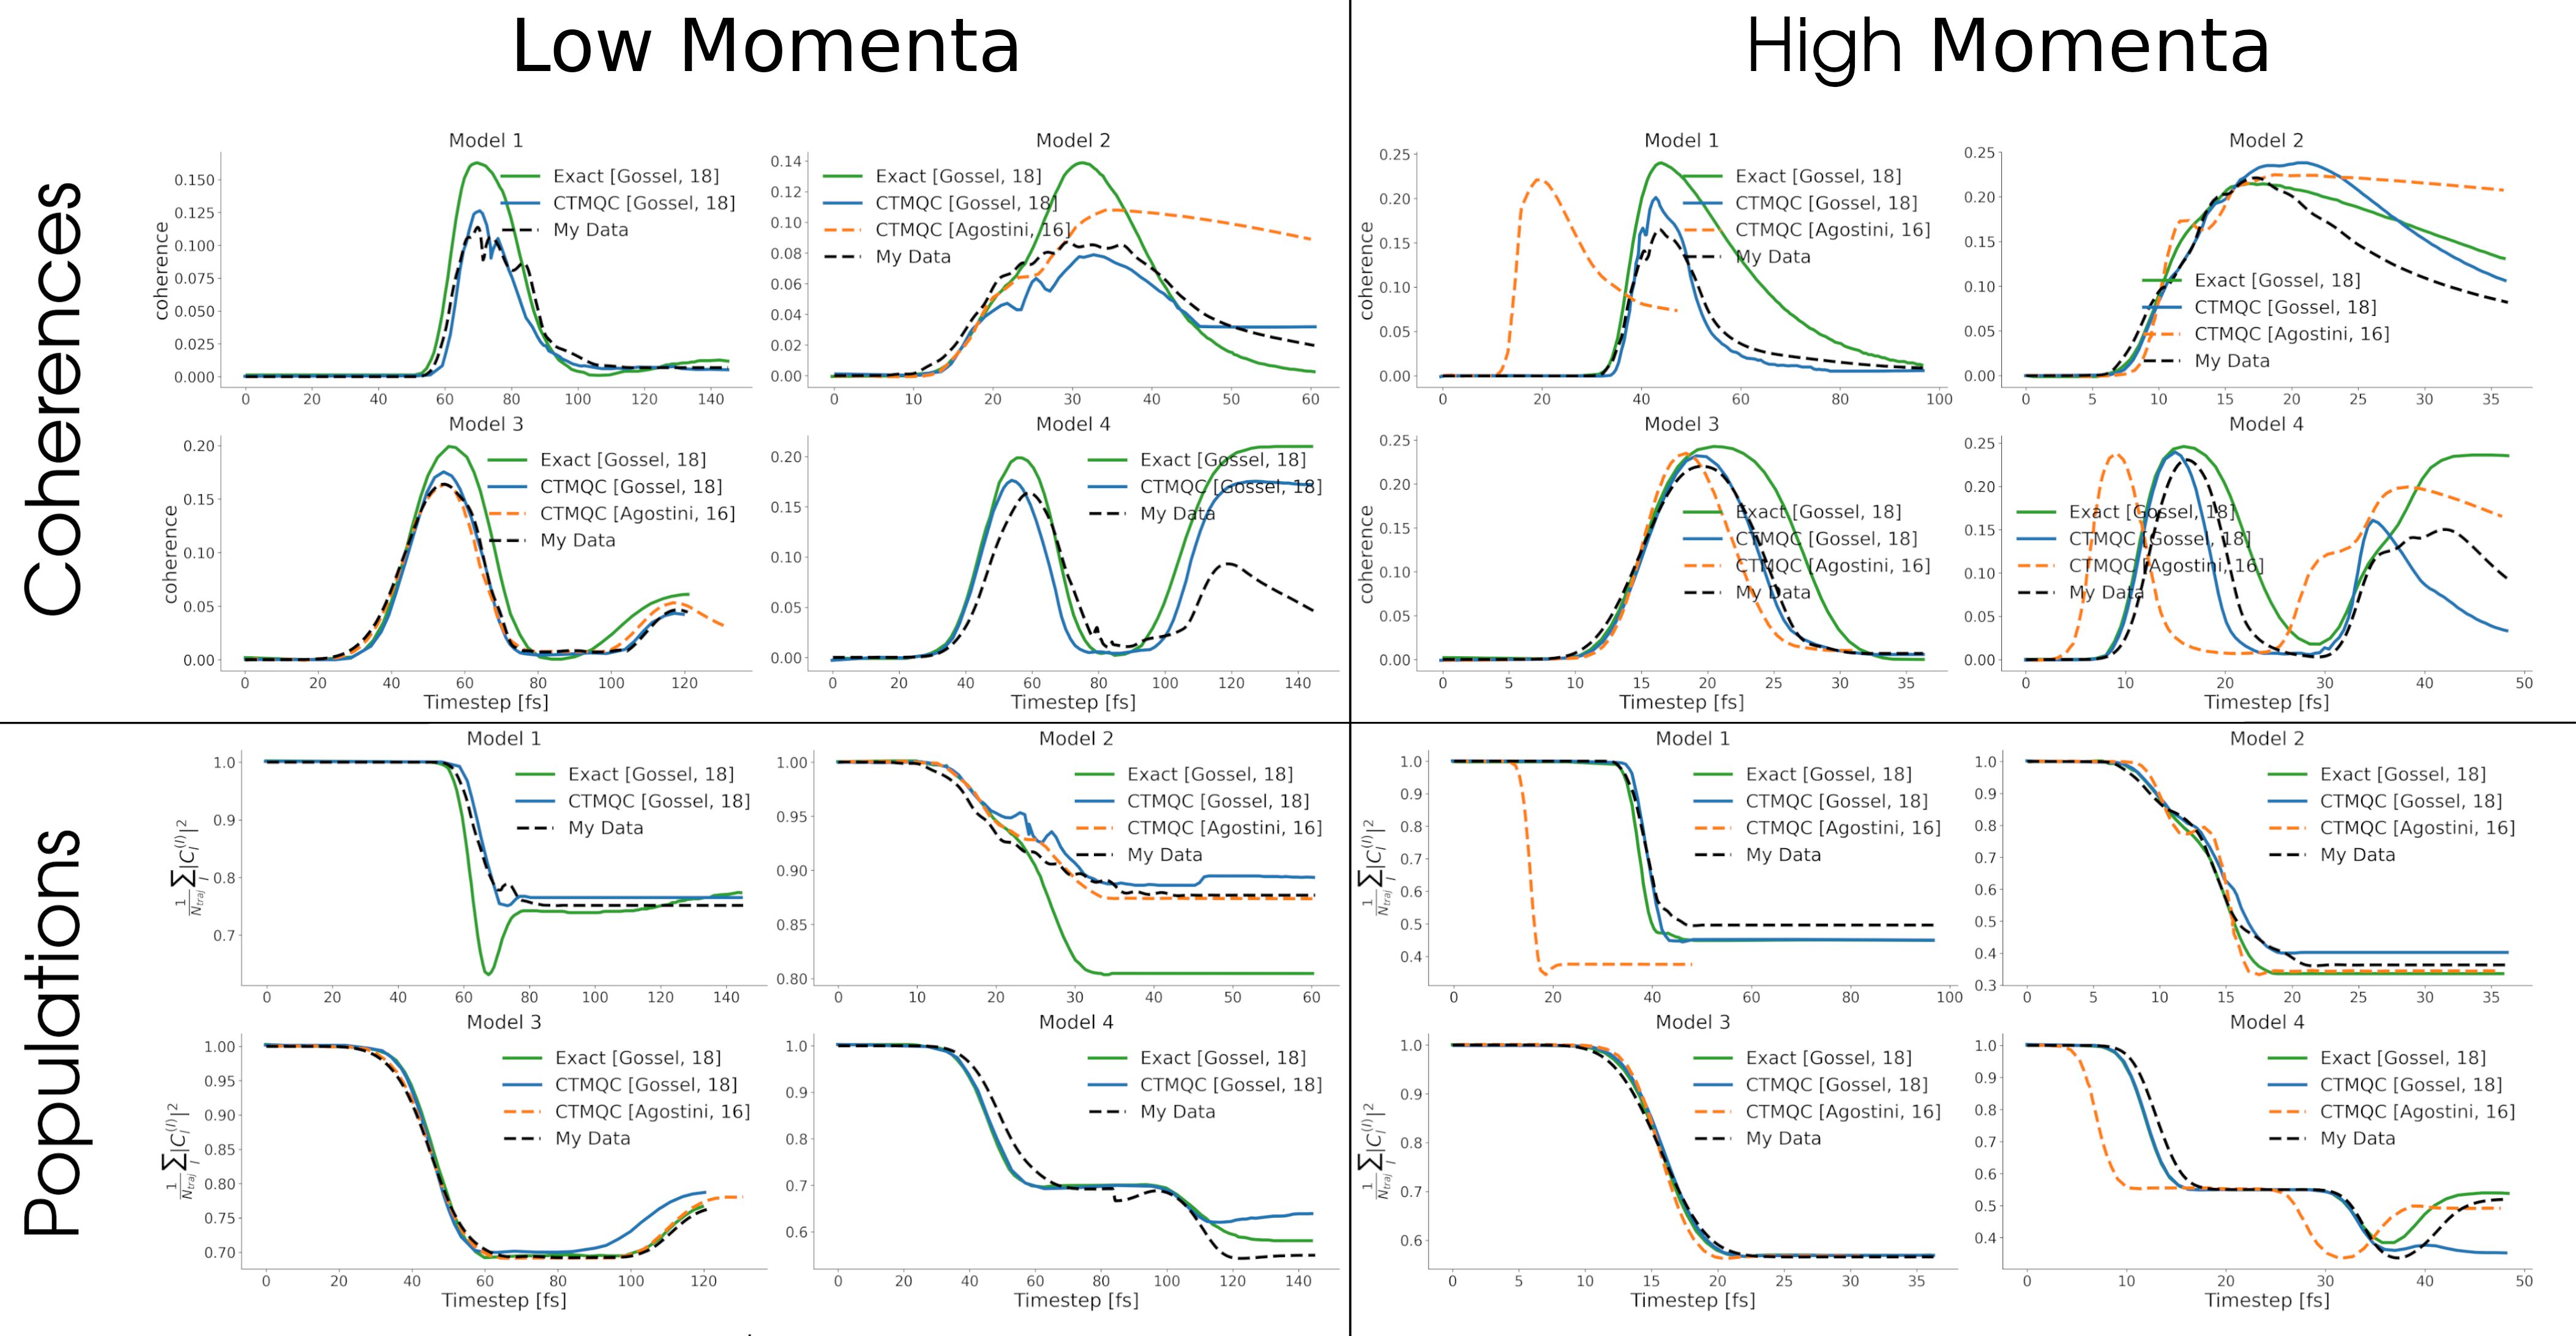
\includegraphics[width=\textwidth]{img/CTMQC/TullyModels/CTMQC_LitComp.png}
	\caption{\label{fig:LitCompCTMQCTully}A comparison of my implementation of full CTMQC (for 4 model Hamiltonians) and results from the literature. The black dashed lines show my CTMQC data (ground state ad pops), the orange dashed lines are data from Agostini, 16 \cite{agostini_quantum-classical_2016} and the blue solid lines are from Gossel, 18 \cite{gossel_coupled-trajectory_2018}. The solid green line shows data from exact quantum mechanical simulations given in Gossel, 18. The figures are labelled with their model number, whether the initial momentum was high or low and whether the populations or coherence indicator was plotted.}
\end{figure}
As in section \ref{sect:EhrenCompare} we can compare the CTMQC results to those published before in Gossel, 18 \cite{gossel_coupled-trajectory_2018} and Agostini, 16 \cite{agostini_quantum-classical_2016}. These results are given in figure \ref{fig:LitCompCTMQCTully}. This time, unlike in the Ehrenfest code, we see some discrepancies between the 3 results which cannot solely be explained as small errors from different sampling of initial positions or from errors in extracting data from graphs in the papers. We can see that the errors mainly appear in the coherence indicator, looking at the bottom row in figure \ref{fig:LitCompCTMQCTully} it appears that both the Agostini and Gossel results match mine (dashed black line) very closely. The largest difference is seen in model 4, high momentum where the Gossel data and mine follow a similar trend and the Agostini data follows the exact curve more closely. The reason for this is a difference in the way the adiabatic momenta terms are handled. In the Gossel paper,  a method to reset the adiabatic momenta to 0 for each replica when the adiabatic populations collapse onto a pure adiabatic state (within a tolerance) is used. If this resetting is turned off then the populations in model 4 follow the Agostini results exactly. While resetting the adiabatic momenta worsens the calculation of the adiabatic populations in the model 4 high momentum simulations, it improves the convergence of the coherence indicator in the model 2 simulations. I will show later how using a  Other deviations in results for the populations are due to a slightly different sampling of initial positions, a different handling of divergences in the quantum momentum term and constructing the $\mathcal{Q}_{lk, \nu}^{(I)}$ term with a different width parameter used to construct the quantum momentum. The differences in my results and those given in the literature are on the same scale as the differences already presented in the literature and they are not large enough to invalidate my implementation. In fact many of the models agree exactly with my implementation and can be taken as a confirmation that my implementation is working. 

\section{Construction of $\mathcal{Q}_{lk, \nu}^{(I)}$}
\label{sect:SigmaSect}
In order to calculate the quantum momentum the nuclear density must be constructed from the nuclei's positions. However, the nuclei are treated classically, i.e. as point particles. To approximate the nuclear density from atomic positions a normal distribution is placed with the mean at position of each particle with a width of $\sigma$ and combined . This method is outlined in the supplementary information on Min, 17 \cite{min_ab_2017} and introduces a new parameter which must be tuned in order to reproduce sensible results. If the width is too small the resulting nuclear density is too noisy and the quantum momentum values unreliable. If the width is too large the nuclear density is very smooth with little variation and the quantum momentum values become very small. Seeing as the quantum momentum is one of the most important factors affecting coherence between electronic states the careful selection of the $\sigma$ parameter is important. This issue is not very well addressed in the literature. In this section I will show results of calculation carried out with various values of $\sigma$ 
as well as a method for a dynamic calculation of $\sigma^{(I)}_{\nu}(t)$ on the fly. In figure \ref{fig:LitCompCTMQCTully} a constant value of 0.35 was used in order to best reproduce the results in Gossel, 18 \cite{gossel_coupled-trajectory_2018}.
\subsection{Constant Values of $\sigma$}
\begin{figure}[ht]
  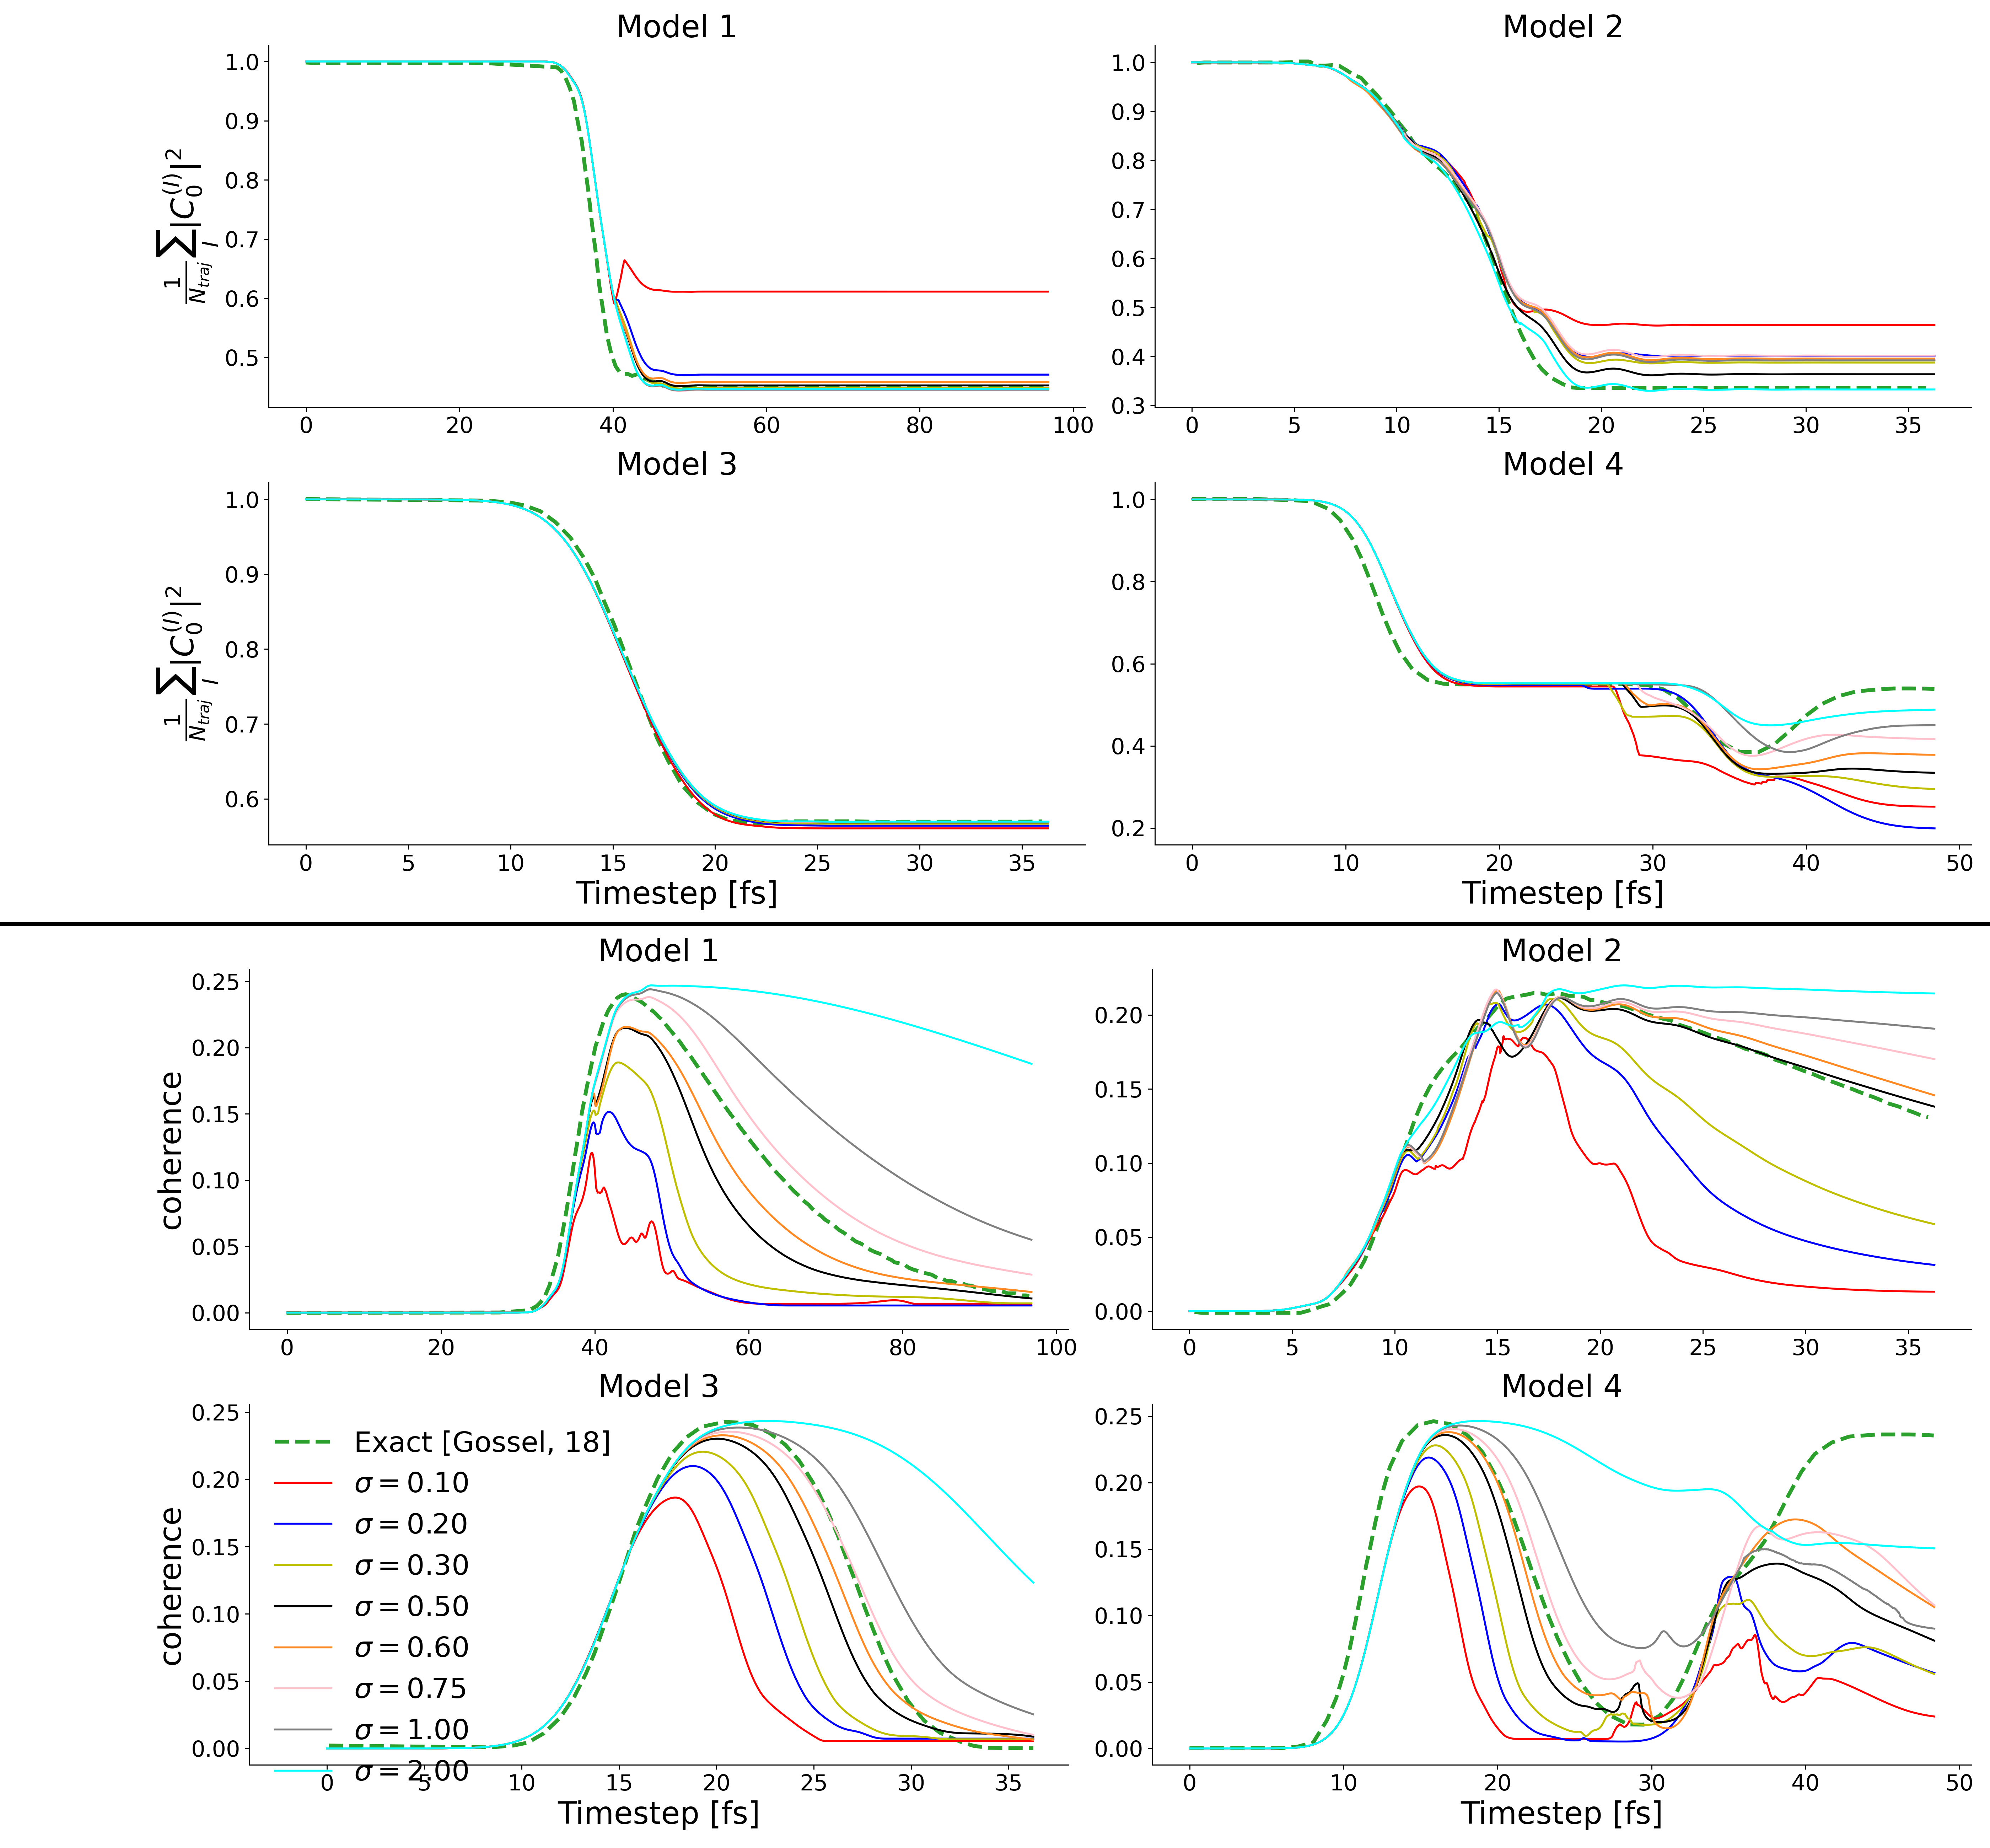
\includegraphics[width=\textwidth]{./img/CTMQC/TullyModels/CTMQC_VarSig_highMom.png}
  \caption{\label{fig:VaryingSigmaTullyModels}4 high momenta cases of the Tully models with a various constant $\sigma$ values used in the calculation of the quantum momentum. Thin solid lines show results from my simulations. The thick, green, dashed line shows data from exact simulations taken from Gossel, 18 \cite{gossel_coupled-trajectory_2018}.}
\end{figure}
\noindent The simplest option for the calculation of $\mathcal{Q}_{lk, \nu}^{(I)}$ is to keep the gaussian width parameter, $\sigma$, constant throughout the simulation. This also allows us to investigate the role of $\sigma$ within the simulations and to determine its influence on the dynamics. To this end various simulations were carried out on the 4 Tully models with the high initial momentum. In each simulation parameters were all the same apart from the value of $\sigma$ which took a value of either: 0.1, 0.2, 0.3, 0.5, 0.6, 0.75, 1 or 2 bohr. The results for these simulations are shown in figure \ref{fig:VaryingSigmaTullyModels}. In this figure, we see that as the $\sigma$ parameter is increased the levels of decoherence also increases. This means for larger $\sigma$ values electronic populations remain in a mixed state for longer and take more time to collapse onto a single adiabatic state. Clearly, the construction of this $\sigma$ parameter is important for recovery of correct electronic dynamics. Surprisingly, this doesn't seem to have much of an effect on the resulting populations. However, this is due to the fact in the limit of large $\sigma$ CTMQC becomes identical to Ehrenfest dynamics and Ehrenfest dynamics captures the evolution of the adiabatic populations very well for each model, with the exception of model 4. It should also be noted that for small values of $\sigma$, propagation using CTMQC can become unstable due to a noisy nuclear density giving rise to an unstable quantum momentum term. A value of 0.6 bohr seems to provide the best fit to exact data. However, this may not mean this is appropriate for all types of simulations.

\subsection{Dynamic $\sigma^{(I)}_{\nu}(t)$ calculation}
\begin{figure}[ht]
  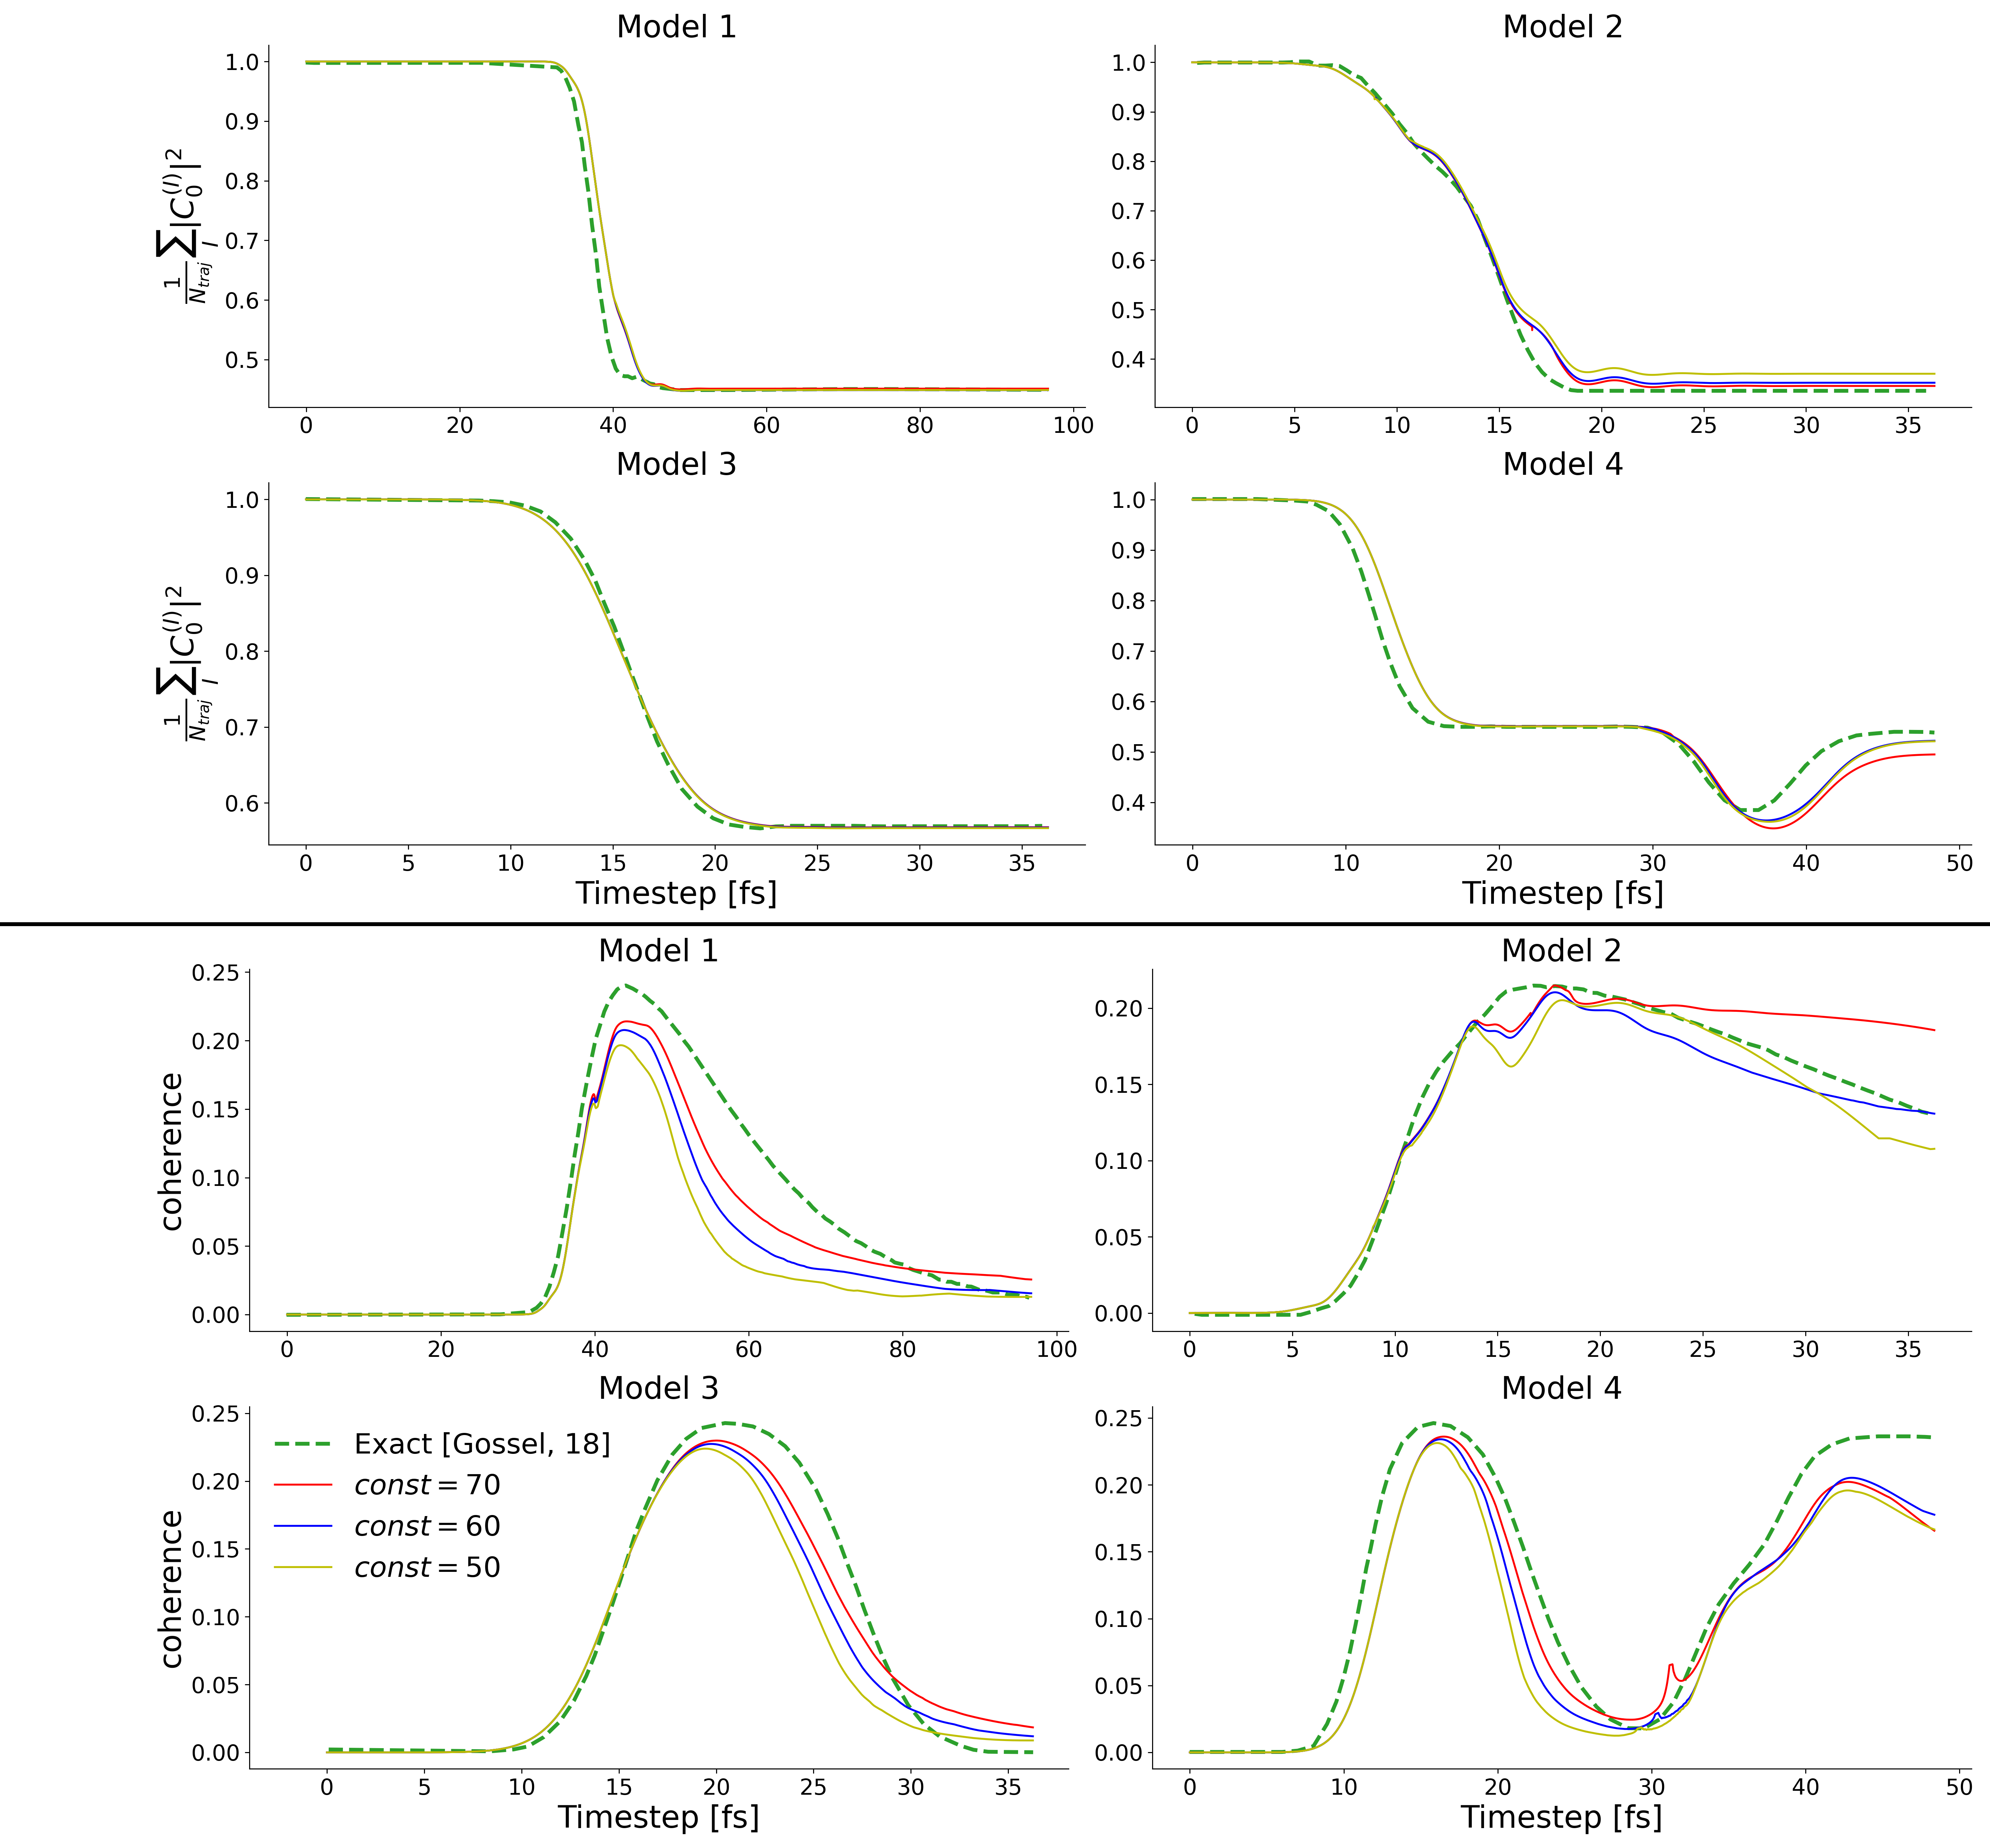
\includegraphics[width=\textwidth]{img/CTMQC/TullyModels/CTMQC_dynSig_highMom.png}
  \caption{\label{fig:dynamicSigma}}
\end{figure}
In the appendix of Gossel, 18 \cite{gossel_coupled-trajectory_2018} an algorithm was outlined to calculate $\sigma$ on-the-fly based on the density of replicas within a cutoff distance of each atom. This is given in appendix \ref{ap:DynamicSigma}. However, this method also relies on a constant parameter to calculate $\sigma$ so doesn't remove a parameter, though the resulting dynamics do not seem as sensitive to changes in this parameter as in $\sigma$ itself.
\\\\
Figure \ref{fig:dynamicSigma} shows populations and coherences for the 4 (high momentum) Tully models with various values of const. It is encouraging to see populations now resemble exact results more closely. This is especially true in model 4, where the dip in the populations is recovered. All 3 constants give nearly identical populations, though a constant of 60 seems to give results that most closely resemble the exact coherences. However, seeing as this (like the width parameter) is not a physical parameter it is hard to know if this is reasonable for all systems. 
\section{Conclusion}
In this chapter I have reported results from my implementation of the CTMQC equations applied to the Tully models. The Tully models are a set of 4 Hamiltonians dictating the motion of 1 atom in 1 dimension. These models are commonly simulated as they are simple enough to be solved analytically and complex enough to provide a reasonable test for any new nonadiabatic molecular dynamics (NAMD) technique. I have shown results from various tests which validate my implementation and shown how well CTMQC conserves the norm of the wavefunction and total energy, with the latter showing some concerning results. I have also highlighted 2 issues with the dynamics in CTMQC. These are the sudden divergences in the quantum momentum term and the ambiguity surrounding the calculation of the gaussian width parameter, $\sigma$. I have given a method designed to address the former issue, which has been shown to significantly improve the norm conservation. The latter problem has been touched upon in the literature, though no thorough studies have been reported.
\\\\
The propagation of the CTMQC equations using a model Hamiltonian is a good first step in implementing a new NAMD technique. It's relative simplicity allows for a close inspection of each of the quantities involved in the propagation, especially new quantities such as the adiabatic momentum term, $\mathbf{f}_{l, \nu}^{(I)}$ and the quantum momentum term, $\mathcal{Q}_{lk, \nu}^{(I)}$. The same code used to simulate the Tully model system can also be used as a base for future extensions such as in 3D or many atom systems. However, before such extensions are implemented a new way to construct the Hamiltonian is needed. In the next chapter I will discuss my implementation of CTMQC within the fragment orbital based framework which relies on the fast calculation of the Hamiltonian using a finite difference method for off-diagonals and a classical force-field to calculate diagonal terms. 




\chapter{CTMQC applied to molecular systems}
\label{chap:molecular_systems}
In order to apply CTMQC to large molecular systems (hundreds of molecules) a different way to construct the Hamiltonian is needed. In this work I have implemented the CTMQC equations within the fragment-orbital based framework. This relies on the equations being expressed in a pseudo-diabatic basis and the Hamiltonian being constructed in two parts: the diagonal elements (site energies) and the off-diagonals (electronic couplings). The basis is termed `pseudo-diabatic' due to the fact that non-adiabatic coupling vectors are small but non vanishing, this results in a basis where the excess charge carrier is strongly but not strictly localised on a single molecule. Within the Hamiltonian, the site energies (diagonal elements) are calculated via classical force-fields and the electronic couplings (off-diagonals) are calculated via the analytic overlap method \cite{gajdos_ultrafast_2014, spencer_fob-sh:_2016} (AOM). In this method the coupling elements are assumed to be proportional to the overlap between the highest singly occupied molecular orbitals (SOMO) on the donor and acceptor molecules (see equation \eqref{eq:AOM_proportional}). This approximation is often used in the literature, e.g. in the fragment orbital density functional theory \cite{KirkpatrickJ2008,C2CP41348E,TroisiA2002} (FODFT) method and has been shown to be valid for many $\pi$-conjugated molecules \cite{KubasA2014, gajdos_ultrafast_2014}.
\begin{equation}
  H_{ab} = C \langle \varphi_{a} | \varphi_{b} \rangle = C S_{ab}
  \label{eq:AOM_proportional}
\end{equation}
Where $\varphi_{a(b)}$ represents a singly occupied molecular orbital on the donor (acceptor) and $C$ is the scaling constant and comes from DFT parameterisation. The singly occupied molecular orbitals are calculated as a linear combination of Slater-type orbitals (STO) as in equation  \eqref{eq:SOMO_def}. In this equation we loop over each atom in the molecule and sum the size of the contribution, $c_{p\pi, i}$, multiplied by the STO, $p_{\pi, j}$. In this case the STO is represented by a p-orbital. The size of the p-orbital on each atom, $c_{p\pi, i}$, is parameterised before the simulation with DFT.
\begin{equation}
  | \varphi_{mol} \rangle = \sum_{i \in mol}^{N_{\text{atoms}}} c_{p\pi, i} | p_{\pi, i} \rangle
  \label{eq:SOMO_def}
\end{equation}
Importantly, the AOM method offers a very fast way to calculate the off-diagonal elements of the Hamiltonian via a finite-difference method with an accuracy comparable to that of DFT methods \cite{AOM_vs_HigherOrder}. This has been implemented within an open-source software package named CP2K and is used by a fragment-orbital based surface hopping technique to study large systems of hundreds of molecules. In the next chapter, the surface hopping technique will be discussed in further detail and applied to a system of pentacene molecules in order to investigate charge carrier (hole) transfer within amorphous systems.


\section{Basis Transformation}
In order to use the FOB method, as stated above, the CTMQC equations in the adiabatic basis must be transformed to the diabatic basis. In the following derivation $C_{l}$ will represent the adiabatic expansion coefficient corresponding to state l and $u_{l}$ will represent the orthogonal diabatic expansion coefficients.
\\\\
The CTMQC equations in the adiabatic basis are given below in equation \eqref{eq:adForce} of the forces and \eqref{eq:adCoeff} coefficients:
\begin{align}
  \begin{split}
	  \mathbf{F}_{\nu}^{(I)} = &- \sum_{k} |C_{k}^{(I)}|^2 \nabla_{\nu}E_{k}^{(I)} - \sum_{k, l} C_{l}^{* (I)} C_{k}^{(I)} \left(E_{k}^{(I)} - E_{l}^{(I)} \right) \mathbf{d}_{\nu, lk}^{ad, (I)} \\
	  &- \sum_{l,k} |C_{l}^{(I)}|^2 \left( \sum_{\nu'}^{N_{n}} \frac{2}{\hbar M_{\nu'}} \mathcal{Q}_{\nu', lk}^{(I)} \cdot \mathbf{f}_{l, \nu'}^{(I)} \right)\left[ \mathbf{f}_{k, \nu}^{(I)} - \mathbf{f}_{l, \nu}^{(I)} \right] |C_{k}^{(I)}|^2 
  \end{split}
  \label{eq:adForce}
\end{align}

\begin{align}
  \begin{split}
	\dot{C}_{l}^{(I)} = &-\frac{i}{\hbar} E_{l}^{(I)} C_{l}^{(I)} - \sum_{k} C_{k}^{(I)} \sum_{\nu=1}^{N_{n}} \frac{\mathbf{P}_{\nu}^{(I)}}{M_{\nu}} \cdot \mathbf{d}_{\nu, lk}^{ad, (I)} \\
	&- \sum_{\nu=1}^{N_{n}} \sum_{k} \frac{\mathcal{Q}_{\nu, lk}^{(I)}}{\hbar M_{\nu'}} \cdot \left[\mathbf{f}_{k, \nu}^{(I)} - \mathbf{f}_{l, \nu}^{(I)} \right] |C_{k}^{(I)}|^2 C_{l}^{(I)}
  \end{split}
  \label{eq:adCoeff}
\end{align}

\noindent Where:
\begin{itemize}
  \item $E_{l}^{(I)}$ is the adiabatic energy for state l and trajectory I
  \item $C_{k}^{(I)}$ is the adiabatic expansion coefficient for state k and trajectory I
  \item $\mathbf{P}_{\nu}^{(I)}$ is the classical momentum of atom $\nu$ on trajectory $I$
  \item $\mathbf{d}_{\nu, lk}^{ad, (I)}$ is the nonadiabatic coupling vector (given in the adiabatic basis)
  \item $M_{\nu}$ is the mass of nucleus $\nu$
  \item $\mathcal{Q}_{\nu, lk}^{(I)}$ is the quantum momentum vector for atom $\nu$ corresponding to the $lk$ pair of states in trajectory $I$
  \item $\mathbf{f}_{l, \nu}^{(I)}$ is the adiabatic impulse on state l, atom $\nu$ and trajectory $I$
\end{itemize}

\subsection{Coefficients}
To transform the equation for the propagation of the coefficients it is far neater to use the matrix notation as in equation \eqref{eq:LA_Coeff} below:
\begin{equation}
	\dot{\mathbf{C}}^{(I)} = \mathbb{X}_{\nu}^{(I)} \mathbf{C}^{(I)} = \left(\mathbb{X}_{eh, \nu}^{(I)} + \mathbb{X}_{qm, \nu}^{(I)}\right) \mathbf{C}^{(I)}
	\label{eq:LA_Coeff}
\end{equation}
Where the $\mathbb{X}$ matrices are defined as in equations \eqref{eq:Xeh_def} and \eqref{eq:Xqm_def} below.
\begin{equation}
  \mathbb{X}_{lk, \nu}^{eh (I)} = -\frac{i}{\hbar} E_{l}^{(I)} - \sum_{\nu}^{N_{n}}\frac{\mathbf{P}_{\nu}^{(I)}}{M_{\nu}} \cdot d_{lk, \nu}^{ad, (I)}
  \label{eq:Xeh_def}
\end{equation}

\begin{equation}
  \mathbb{X}_{ll, \nu}^{qm (I)} = -\sum_{\nu=1}^{N_{n}} \sum_{k} \frac{\mathcal{Q}_{\nu, lk}^{(I)}}{\hbar M_{\nu'}} \cdot \left[ \mathbf{f}_{k, \nu}^{(I)} - \mathbf{f}_{l, \nu}^{(I)} \right]  |C_{k}^{(I)}|^2
  \label{eq:Xqm_def}
\end{equation}
The subscript $ll$ in equation \eqref{eq:Xqm_def} indicate that these values occur only along the diagonal of the matrix $\mathbb{X}^{qm (I)}$

\noindent Using the identities:
\begin{align}
  \mathbb{U}^{-1} &= \mathbb{U}^{\dagger} \\
  \mathbf{C}^{(I)} &= \mathbb{U}^{\dagger (I)} \mathbf{u}^{(I)} \\
  \dot{\mathbf{C}}^{(I)} &= \dot{\mathbb{U}^{\dagger (I)}} \mathbf{u}^{(I)} + \mathbb{U}^{\dagger (I)}\dot{\mathbf{u}}^{(I)}
\end{align}
Where $\mathbb{U}^{(I)} = \langle \phi_{l}^{(I)} | \psi_{n}^{(I)} \rangle$ is the unitary transformation matrix transforming from the diabatic to adiabatic basis. The $\mathbf{u}^{(I)}$ terms are the diabatic expansion coefficients on trajectory I.
\\\\
\noindent After some algebra we arrive at:
\begin{equation}
  \dot{\mathbf{u}}^{(I)} = \underbrace{\left(\mathbb{U}^{(I)} \mathbb{X}_{eh} \mathbb{U}^{\dagger (I)} + \mathbb{U}^{(I)}\mathbb{U}^{\dagger (I)}\right) \mathbf{u}^{(I)}}_{\text{Ehrenfest}} + \underbrace{\left(\mathbb{U}^{(I)} \mathbb{X}_{qm} \mathbb{U}^{\dagger (I)} \right) \mathbf{u}^{(I)}}_{\text{Quantum Momentum}}
  \label{eq:diabMatEq}
\end{equation}
In equation \eqref{eq:diabMatEq} I've separated the contribution from Ehrenfest and the contribution from the new quantum momentum terms. The Ehrenfest part can be shown to reduce to a simpler form (see Spencer, 2016 \cite{spencer_fob-sh:_2016} and Carof, 17 \cite{carof_detailed_2017} for more details). The quantum momentum term must be coded up as shown with the transformation matrices. This gives the final equation for the propagation of the diabatic expansion coefficients, shown in equation \eqref{eq:DiabPropagation}.
\begin{equation}
	\dot{\mathbf{u}}^{(I)} = \left(-\frac{i}{\hbar} \mathbb{H}^{(I)} - \mathbb{D}^{(I)}_{diab} \right) \mathbf{u}^{(I)} + \left(\mathbb{U}^{(I)} \mathbb{X}_{qm} \mathbb{U}^{(I)})^{\dagger} \right) \mathbf{u}^{(I)}
  \label{eq:DiabPropagation}
\end{equation}
Where $\mathbb{H}^{(I)}$ is the diabatic Hamiltonian constructed via the AOM method, $\mathbb{D}_{diab}^{(I)}$ are the diabatic nonadiabatic coupling elements ($d_{diab, lk}^{(I)} = \langle \phi_{l} | \dot{\phi}_{k} \rangle$).

\subsection{Forces}
A full derivation of the transformation of basis for the equation propagating forces is given in appendix \ref{ap:BasisTrans}. The result is given in equation \eqref{eq:diabForces} below:
\begin{align}
  \begin{split}
	  \mathbf{F}_{eh, \nu}^{(I)} &= \sum_{i,j} \mathbf{u}_{i}^{*(I)} \mathbf{u}_{j}^{(I)} \left( \nabla_{\nu} H_{ij}^{(I)} + \sum_{l} \mathbf{d}_{lk, \nu}^{(I)} H_{lj}^{(I)} - \sum_{l} \mathbf{d}_{lj, \nu}^{(I)} H_{il} \right) \\
	  &- \sum_{l,k} |C_{l}^{(I)}|^2 \left( \sum_{\nu'}^{N_{n}} \frac{2}{\hbar M_{\nu'}} \mathcal{Q}_{\nu', lk}^{(I)} \cdot                   \mathbf{f}_{l, \nu'}^{(I)} \right)\left[ \mathbf{f}_{k, \nu}^{(I)} -          \mathbf{f}_{l, \nu}^{(I)} \right] |C_{k}^{(I)}|^2
	\end{split}
  \label{eq:diabForces}
\end{align}
Where the definitions of the terms within equation \eqref{eq:diabForces} have been explained previously.

\noindent There are a couple of things to note with this equation. Firstly, (as in the coefficients equation) the quantum momentum part has not been transformed. This is because the forces are basis independent and don't need to be transformed. Secondly, the quantities required for the calculation of this part of the equation are already calculated in order to propagate the coefficients so only a small amount of extra effort is required to calculate the quantum momentum force term. The Ehrenfest part of the equation has been transformed. This is because the nonadiabatic coupling vectors within the adiabatic basis are never required so are never calculated. The Ehrenfest force term requires these nonadiabatic coupling vectors so would add an extra computational overhead. Further, the commutator term in the diabatic basis has been observed to provide a negligible contribution to the overall force in previous simulations (not shown in this work). This term requires significant computational effort and can be neglected. This makes the calculation of the Ehrenfest forces in the diabatic basis far cheaper than in the adiabatic basis.

\section{Testing the diabatic propagator}
The diabatic propagation can be tested against the already tested adiabatic propagator using the Tully model Hamiltonian. The code should give the same results, given the same inputs. To check this, in figure \ref{fig:diab_prop_vs_adiab}, the simulations carried out in figure \ref{fig:LitCompCTMQCTullyHigh} were repeated though this time the diabatic propagator was used.
\begin{figure}[ht]
  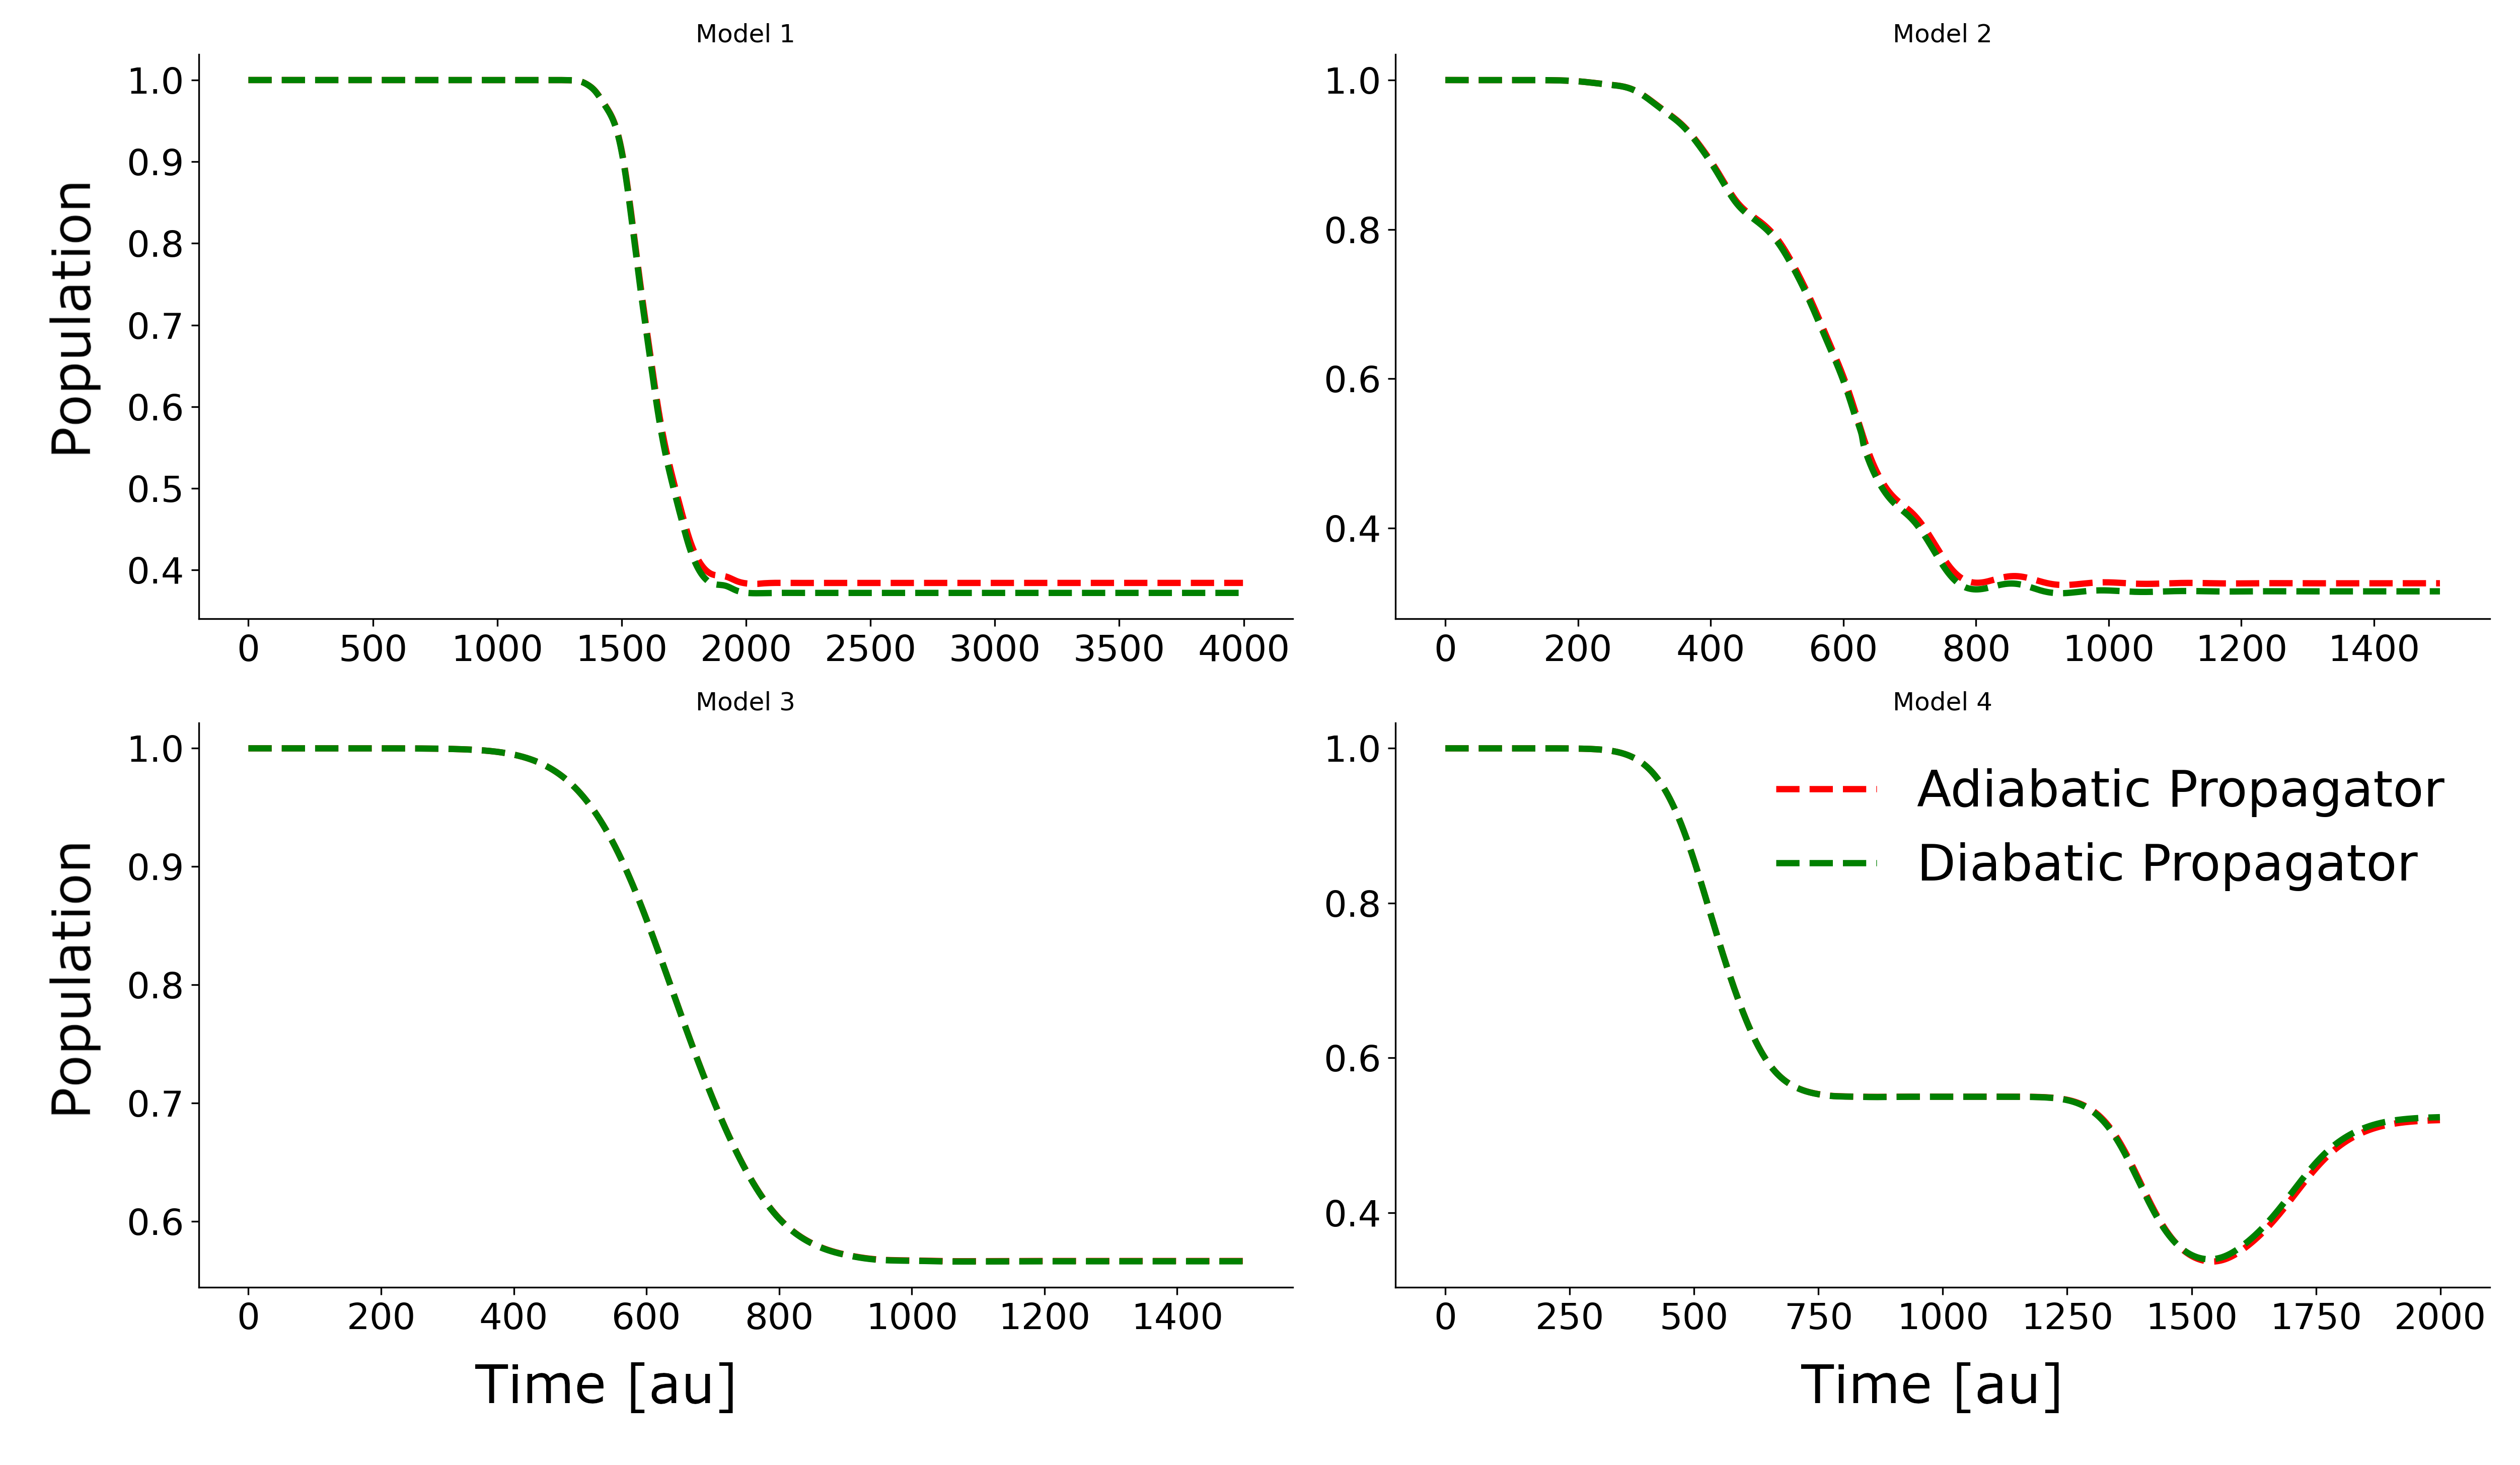
\includegraphics[width=\textwidth]{../img/CTMQC/TullyModels/CTMQC_ad_vs_di_wTraj_pops.png}
	\caption{\label{fig:diab_prop_vs_adiab}The four Tully models simulated using propagating the equations within a diabatic and adiabatic basis. The green line shows results from the diabatic propagator and the red line shows results from the adiabatic propagator. Model three shows an exact agreement between the adiabatic and diabatic propagators hence only one line is seen.}
\end{figure}
We can see in figure \ref{fig:diab_prop_vs_adiab} that the results for the adiabatic and diabatic propagator are almost exactly the same for each model. In model three, where the problem with the divergent $\mathcal{Q}_{lk, \nu}^{(I)}$ doesn't occur, the two results are exactly on top of each other. In the other models there is a slight discrepancy. This is due to the unpredictable $\mathcal{Q}_{lk, \nu}^{(I)}$ spikes not being perfectly corrected. However, figure \ref{fig:diab_prop_vs_adiab} still serves as confirmation of the propagation within the diabatic basis.

\section{Simulating Molecular Systems}
To go beyond the 1D Tully model systems the AOM method is combined with CTMQC and applied to an Ethylene dimer. Fortunately, the majority of the code from the Tully model systems can be re-used. In fact, the only difference is the way the Hamiltonian (and diabatic NACE) is constructed. The code for carrying out these tasks (the AOM part) has been implemented by previous members of the group and has been well tested and verified against the literature and experimental studies. Therefore, I will not include any tests of this part of the code in this document but instead refer the reader to the numerous papers discussing AOM and its use in within the fewest switches surface hopping framework \cite{Carof2017FSSH, C9FD00046A, C9CP04770K, FOB-SH_Spencer, C6FD00107F,FlickPolarons, Giannini2018Crossover, Giannini2019, C9TC05270D,Gajdos2014, AOM_vs_HigherOrder}. An ethylene dimer was chosen as a reasonable first system due to its relative simplicity (shown in figure \ref{fig:EthDimer}) the total number of atoms is twelve and only two electronic states will be considered.
\begin{figure}[ht]
  \includegraphics[width=\textwidth]{../img/CTMQC/Ethylene_Annotated.png}
	\caption{\label{fig:EthDimer}An example Ethylene dimer used to test the CTMQC implementation. The right panel shows the positions of just one replica. The left panel shows the positions of all replicas with the replica shown on the right highlighted in red.}
\end{figure}
The system shown in figure \ref{fig:EthDimer} was initialised in the adiabatic ground state. Positions and velocities were sampled from a short NVT molecular dynamics equilibration. The scaling factor ($C$ in equation \eqref{eq:AOM_proportional}) was chosen to give a coupling of approximately 27 meV. This is approximately $\frac{1}{4} \times$ the reorganisation energy parameterised to be 100 meV. The amount of charge transfer is dependent on the ratio between reorganisation energy and the electronic couplings ($\frac{H_{ab}}{\lambda}$). The factor of $\frac{1}{4}$ was chosen to be a reasonable factor seen in other organic semiconducting systems. The nuclear timestep was chosen to be 0.05fs and the electronic one was 0.005 fs. The switch to $\mathbf{R}_{0, \nu}^{(I)}$ was chosen as the correction method of the quantum momentum and 100 trajectories were used. A constant $\sigma$ of 0.7 was used as the dynamic $\sigma$ tended to either vanish to zero or blow up to a very large number.
\\\\
In figure \ref{fig:CP2K_norm} the norm of the diabatic expansion coefficients are plotted, from the system described above. In this figure we see large jumps in the norm, these are caused by the divergences in the quantum momentum term. These occur more in this system than in the Tully models as it is more complex (more atoms, higher dimensional) and runs for a longer time with more avoided crossings. The fact that there are twelve atoms and three Cartesian dimensions instead of one means that the $\mathbf{R}_{lk, \nu}$ term must be calculated many more times increasing the probability of happening upon a divergence. For example, the Tully models tended to run for 10s of fs and had one value of $\mathbf{R}_{lk, \nu}$. The Ethylene dimer typically runs for 100s of fs encountering 10s of avoided crossings with 36 unique values of $\mathbf{R}_{lk, \nu}$. The errors can also accumulate meaning that after a few trivial crossings the populations become extremely noisy. This eventually causes the code to crash and results from it cannot be trusted. Most commonly the reason for the code crashing is a large spike in the computed forces caused by a spike in the quantum momentum. This large force then causes the atoms to collide and the code to crash. The code is very stable when just using Ehrenfest dynamics.
\begin{figure}[ht]
  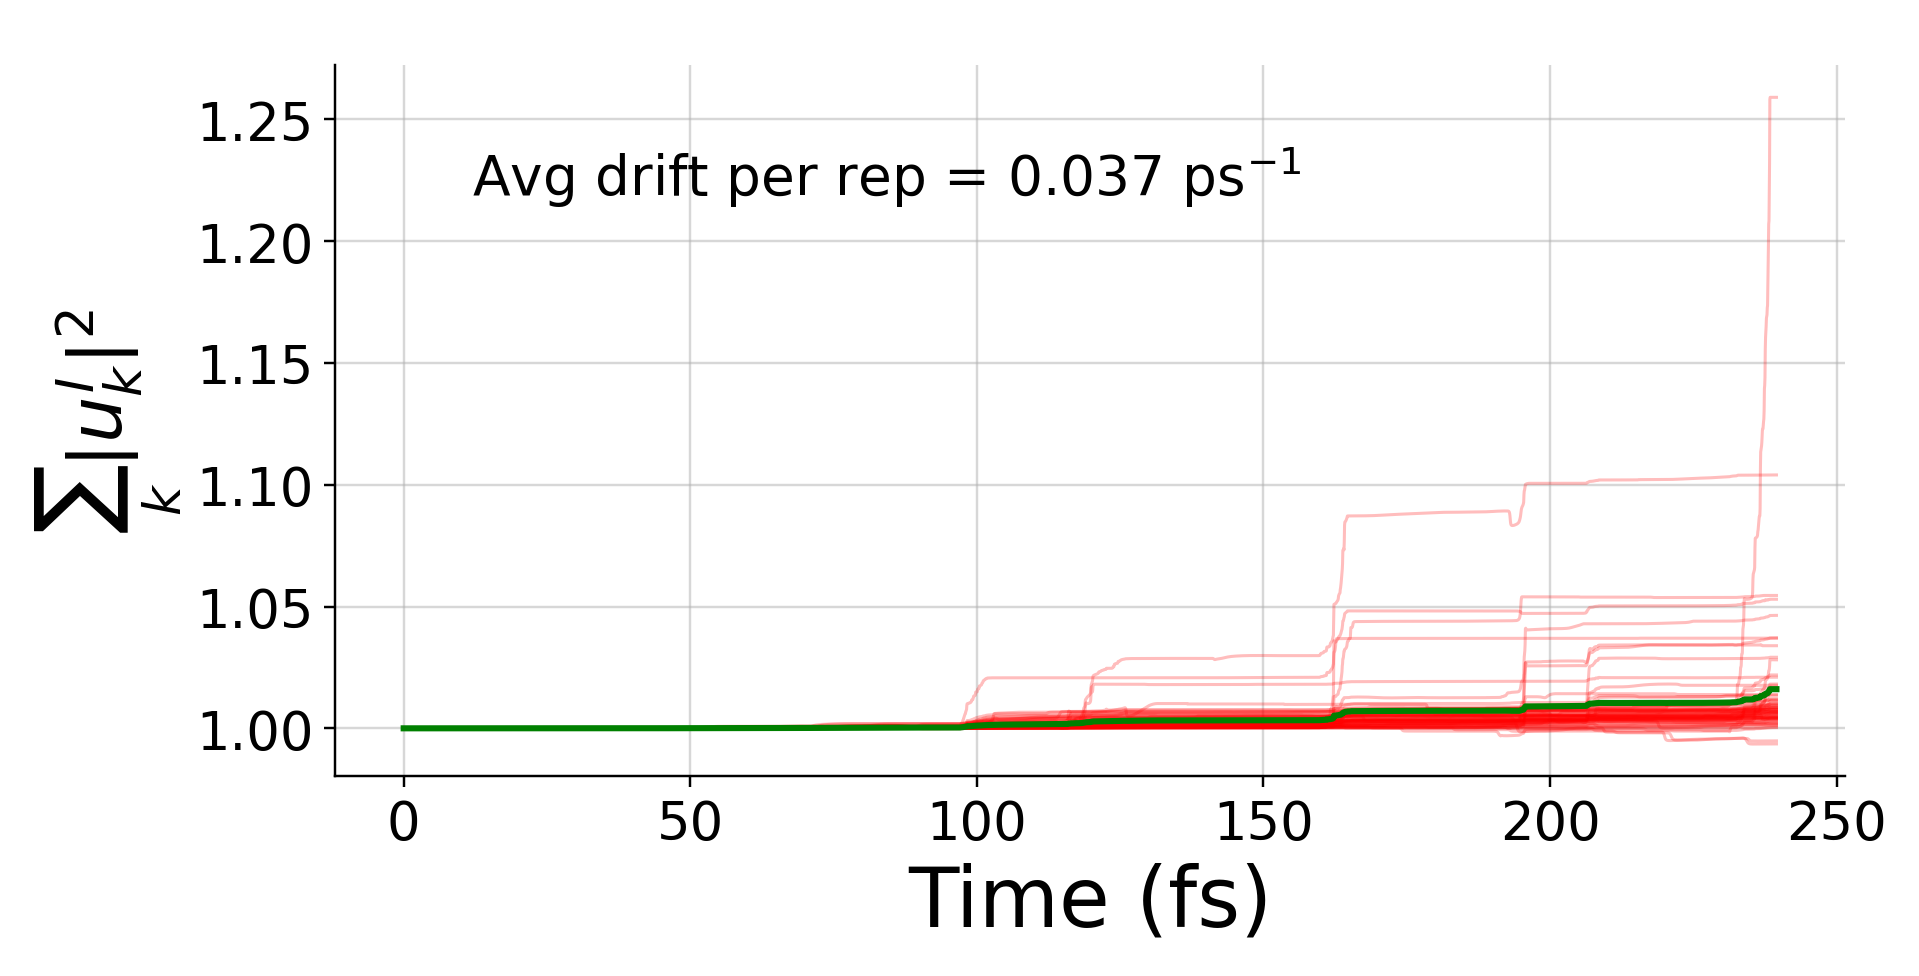
\includegraphics[width=\textwidth]{../img/CTMQC/Ethylene_norm.png}
  \caption{\label{fig:CP2K_norm}The norm of the adiabatic expansion coefficients. Thin red lines show the norm for each trajectory and the thick green line shows the average over all trajectories.}
\end{figure}
Many more simulations have been carried out to diagnose and fix this issue. Results from all of these cannot be included in this document though I will provide a brief summary of results below.
\\
\begin{itemize}
	\item \textbf{Varying the number of replicas}: Increasing the number of replicas in the system, somewhat counterintuitively, decreases stability. This is because with more replicas there is more of a chance the code will stumble upon a calculation giving a divergence in the quantum momentum term.
	\item \textbf{Varying the timestep}: Decreasing the timestep does help to improve norm conservation (before the code crashes). However, it does not lead to a more stable simulation that allows for longer timescales to be simulated. This is because decreasing the timestep provides more opportunity for a small numerical error to cause a divergence in the quantum momentum term.
	\item \textbf{Removing Center of Mass Motion}: In some simulations the replicas positions spread out so much that the quantum momentum term became negligible. This was to prevent that from happening.
	\item \textbf{Varying the gaussian width ($\sigma$) parameter}: If the $\sigma$ parameter is set to be large (> 2) then the simulation is more stable as the quantum momentum term is smaller and errors don't accumulate as quickly. However,  the limit of a very large $\sigma$ is Ehrenfest dynamics. If the $\sigma$ is set to be small (< 0.2) the simulation becomes extremely unstable as the quantum momentum forces populations to decohere too quickly. This is discussed in more detail in section \ref{sect:SigmaSect}.
	\item \textbf{Turning off the quantum momentum addition to the force term}: The code runs more stably if the quantum momentum term is not included in the forces. This has also been shown to be much less important for the accuracy of the results than the quantum momentum addition to the coefficients. However, even in this case the code eventually crashes after an accumulation of errors in the coefficients results in erroneous forces resulting in geometries that fail CP2K internal checks.
	\item \textbf{Renormalisation}: This does not seem to help with stability. Furthermore, it merely helps hide the large norm drift and doesn't fix the problems it causes.
\end{itemize}
\section{Conclusions}
The CTMQC method shows great promise as a new nonadiabatic molecular dynamics (NAMD) technique. It was derived as the semi-classical limit of the exact factorisation of the time-dependent electron-nuclear wave function \cite{abedi_exact_2010, agostini_semiclassical_2015}. It purports to handle decoherence corrections in a more rigorous, first principles, way without the need of empirical parameters. Although this method was first reported in 2015 \cite{agostini_semiclassical_2015}, there are still very few papers reporting results using this method \cite{min_ab_2017, gossel_coupled-trajectory_2018,agostini_semiclassical_2015}. With the most complex system being restricted to a seven atom molecule simulated for just 10s of fs\cite{min_ab_2017}. In this work, I have transformed the basis of the CTMQC equations, to an orthogonal diabatic basis, and implemented it within the FOB framework. This has allowed me to study to a molecular system (dimer of Ethylene) totalling twelve atoms, simulated for hundreds of fs. However, instabilities in the algorithm have prevented any physical conclusions being drawn from this. Before the widespread acceptance of CTMQC as a standard nonadiabatic molecular dynamics method, two critical flaws must be addressed. First is the calculation of the gaussian width parameter, $\sigma$, and the second is the divergence of the quantum momentum term. It would be possible to further investigate the width parameter, perhaps through benchmarks against higher level calculations to establish a relationship between it and other characteristics of the system. From a short investigation using the Tully models it seems a constant width parameter gives reasonable results and it should be set to be between 0.2 and 0.5. The on-the-fly update of the width parameter, from an algorithm given in Gossel \cite{gossel_coupled-trajectory_2018}, provided even better results that came very close to the exact quantum dynamical values. Therefore, the setting of this width parameter does not seem like an intractable problem. However, it may be harder to correct for the large divergences in the quantum momentum caused by the denominator of the quantum momentum intercept term, $\mathbf{R}_{lk, \nu}$, approaching zero. This causes the code to become unstable for even simple molecular systems. In the 1D Tully models, this could be corrected by switching to an alternative intercept, $\mathbf{R}_{0, \nu}^{(I)}$. The switch occurs after two conditions are satisfied: a threshold on the time-derivative of the $\mathbf{R}_{lk, \nu}$ term has been surpassed and the denominator of the $\mathbf{R}_{lk, \nu}$ term is sufficiently close to zero. The correction helps conserve norm within the Tully model simulations. However, in larger, longer running simulations errors soon accumulate and the code becomes unstable. The Tully models also gave fewer divergences due to smaller run-times and the fact it is a simpler system. The alternative intercept results in unphysical population transfer in regions of zero nonadiabatic coupling, so cannot be used throughout the simulation.
\\\\
Both these problems can both be traced back to the construction of the nuclear density from the nuclear positions. The method explored in this thesis is the method reported in the literature. That involves placing a gaussian function centered on each atomic position with a certain width, $\sigma$ to smear out the (point) position and give a smooth nuclear distribution. I believe that exploring alternative techniques to construct the nuclear density from atomic positions may lead to the largest improvements in the CTMQC technique. Perhaps even allowing one to study complex molecular systems with many nonadiabatic coupling regions such as those typically found in charge transfer studies. 
\\\\
Finally, the algorithm does not seem to conserve total energy. Using the equation for potential energy given in \cite{agostini_semiclassical_2015} we see that even very small nuclear timesteps do not conserve total energy to better than 10$^{-2}$ Ha ps$^{-1}$ atom$^{-1}$ in the best case. For reference, a good energy conservation within classical molecular dynamics is considered to be $\sim 10^{-10}$ or less. Further, and perhaps more concerningly, reducing the timestep does not seem to improve the issue. This would be a major obstacle to CTMQC's widespread adoption as a nonadiabatic molecular dynamics algorithm and further work is needed to address the issue. In the rest of this work I will discuss an alternative NAMD technique, namely fewest switches surface hopping (FSSH), and apply it to large molecular systems to get experimentally verifiable results.
\\\\
I have implemented and tested a working version of CTMQC both in CP2K and as a standalone python script. These are both available for downloading from the author's github page at: \href{https://github.com/95ellismle}{https://github.com/95ellismle}.

\chapter{Charge transfer in amorphous systems}
\label{chap:surface_hopping_app}
Although it is important to know the maximum bound on the mobility of the charge carrier in a perfect crystal of an organic semiconductor, in reality it is very difficult to control defect formation in OSs\cite{NGUYEN2006198,Ray2014}. This is due to van der Waals forces only weakly holding molecules at lattice sites, allowing molecules greater freedom than in traditional inorganic crystal, and increasing the chance of defect formation which can trap/scatter charge carriers\add{, thereby } reducing overall mobility. This means it is important to investigate and characterise charge transport properties for not just perfectly crystalline OSs but also those that show a range of amorphicity.
\\\\
In this chapter I investigate how structural disorder of the OS, on top of thermal disorder, changes the physical nature of the charge carrier, its localization length, transport mechanism and mobility. In particular, the degree of structural disorder at which the flickering polaron loses its delocalized character and becomes localized. This is important because a decrease in charge carrier delocalization correlates with a decrease in charge mobility, the essential result of transient localisation theory. To do so, I present quantum dynamical calculations of the charge carrier dynamics at room temperature in a number of samples of pentacene with varying levels of crystallinity, from fully amorphous to perfectly crystalline. The quantum dynamical simulation method, denoted fragment orbital-based surface hopping (FOB-SH), is well suited for this task because it makes no assumptions with regard to the charge transport mechanism. FOB-SH was shown to predict charge mobilities well over several orders of magnitude but it has so far only been applied to single crystalline OS. Methodological developments by me and other members of the Blumberger group have now made it possible to apply this novel methodology, for the first time, to large samples of disordered OS with different nanoscale morphologies.
\\
\begin{wrapfigure}{r}{0.4\textwidth}
	\vspace*{-0.5cm}
	\includegraphics[width=0.4\textwidth]{../img/herringbone.png}
	\caption{An example of the \\herringbone packing \\typically found in \\Pentacene crystals}
	\label{fig:HerringbonePacking}
\end{wrapfigure}
The molecule under investigation is pentacene. This molecule is a popular organic semiconductor and the subject of much research due to its high field effect mobility \cite{Hu2005}, use in device applications \cite{Hasegawa_2009} and, more recently, the use of functionalization to alter device properties \cite{Anthony2001, Anthony2002}. The pentacene molecule consists of \replace{5}{five} joined benzene rings (\replace{36}{thirty six} atoms) and crystals typically pack with a herringbone motif as shown in figure \ref{fig:HerringbonePacking}.
\clearpage
\section{Creating Amorphous Pentacene}
In order to create the amorphous pentacene systems a melt-quench technique was used. This is a standard technique, often used to create amorphous systems in both computational and experimental  fields \cite{D’Angelo2018, PhysRevB.77.172101, BERBANO201293, KARMWAR201194, KO1996211}. The procedure followed is shown in figure \ref{fig:meltQuenchFlowChart}.
\begin{figure}[H]
	\includegraphics[width=\textwidth]{../img/FlowCharts/MeltQuench.png}
	\caption{\label{fig:meltQuenchFlowChart}The melt-quench scheme used to create amorphous pentacene systems. Blue boxes indicate steps using an NPT ensemble, orange boxes indicate use of a NVT ensemble.}
\end{figure}
\noindent In this procedure, the system was initialised with an individual pentacene molecule on a regular \replace{3D}{three dimensional} grid using an orthorhombic unit cell. This was chosen to make analysis of the resulting structures easier than with the triclinic unit cell typically used to simulate pentacene crystals. The velocities were initially randomly sampled from a gaussian distribution and a Nose-Hoover thermostat and barostat was used to control the temperature and pressure. The Lammps molecular dynamics package was used \cite{LammpsMain, LammpsURL} and electrostatic interactions were handled with Lammps' particle-particle-particle-mesh ewald method \cite{LammpsPPPME}. RESP \cite{RESP} (restrained electrostatic potential) partial charges were parameterised using Gaussian 16 \cite{g16} with the B3-LYP\cite{B3,LYP} level of theory and a 6-311g(d) basis set. The use of partial charges was essential in the creation of the amorphous systems and neglecting them lead to unphysical face-to-face stacking of pentacene molecules. This is shown in figure \ref{fig:glob_coup}, in section \ref{sect:GlobCoup}. Finally, for inter and intra molecular interactions the general AMBER force-field \cite{GAFF} (GAFF) was applied. There isn't one predominant forcefield used in simulations of pentacene in the literature, though parameters from GAFF have been used and validated in a number of studies \cite{C0JM01577F, Yoneya2012, PentCrystallisation, MILLER201728, Wang2011, C6CP06436A, doi:10.1246/cl.180450}.
\\\\
Four different quenching times were used spanning \replace{4}{four} orders of magnitude: 0ns, 1ns, 10ns and 100ns. For the 0ns, 1ns and 10ns quenching simulations \replace{3,000}{three thousand} molecules were simulated. In the 100ns quenched structure \replace{3060}{three thousand and sixty} molecules were simulated. The initial structure for the 1ns and 10ns quenched structures were taken from a restart of the 0ns quenched simulation after the 800K equilibration step. The 0ns and 1ns quenched structure were carried out under \replace{1}{one} atmosphere of pressure in x, y and z. However, the 10ns quenching required a small increase to \replace{5}{five} atmospheres as the structure had a tendency to deform such that one of the cell vectors became either very large or very small. In the 100ns quenched structure I updated the barostat target pressure (before the phase transition) to account for similar deviations in simulation box dimensions.
\section{Structure of the quenched simulations}
A movie showing the full 100ns melt-quench simulation can be found here: \href{https://youtu.be/6IQcYErQHVs}{https://youtu.be/6IQcYErQHVs}. Still images of the final snapshot of each different quenching time are shown in figure \ref{fig:final_snapshots}.
\subsection{Final Structure Snapshots}
\noindent We can see qualitatively that as we increase the quenching time from a) $\rightarrow$ d) the structure starts to look more ordered and crystal layers are starting to be formed. Looking longer at the structure we see that lower quench times tend to form small crystal clusters. In the 0ns quenched structure these clusters tend to be just $\sim$\replace{7-10}{seven to ten} molecules in size. As we increase the quenching time to 1ns we see \replace{1D}{one dimensional} channels of crystalline pentacene start to form throughout the structure, though the structure is still relatively disordered due to these channels being randomly oriented with respect to one another. As we increase the quenching time these crystal fragments become larger until in the 100ns quenched structure the whole system is comprised of just \replace{2}{two} crystals. The reason for this is, as the rate of cooling is decreased, the rate of crystal seeding is also decreased. At longer quenching times, more spent is spent at a temperature where it is unlikely for crystal to start to form --so fewer form. Those that do form can therefore propagate through the full system before being impeded by others. This can be seen in the animation of the \href{https://youtu.be/6IQcYErQHVs}{100ns melt quench simulation} linked above. The reverse is true for the shorter quenching times. In these systems, we quickly pass into a state that's energetically favourable for many crystals to start to form. These all propagate out at random orientations with respect to each other and block each other's growth.

\begin{figure}[ht]
	\includegraphics[width=\textwidth]{../img/DifferentQuenchTimes/AllTimes.png}
	\caption{\label{fig:final_snapshots}The final snapshot of each quenching simulation visualised in VMD \cite{VMD} and rendered with Tachyon \cite{Tachyon}. Snapshots are ordered by quenching time i.e. a) is the 0ns quench, b) is the 1ns quench and so on.}
\end{figure}
\subsection{Molecular Packing}
\noindent We can isolate clusters in each of the different structures shown in figure \ref{fig:final_snapshots} to reveal the molecular packing within. In figure \ref{fig:Layer11} \replace{a}{an algorithm similar to the density-based spatial clustering of applications with noise (DBSCAN) one} \cite{DBSCAN}\mremove{-like algorithm} has been applied to the final structure from the 100ns quench to cluster molecules based on the density of centers of mass of molecules. These clusters have then been highlighted by different colours. The top-most green cluster has been rotated such that, on the left, we are viewing it at an angle perpendicular to the plane of molecules, as shown by the cartoon eye. Comparing this plane to the crystal plane to the right, we can see a striking similarity in the packing motif. The herringbone packing has formed and (as can be seen in figure \ref{fig:ang_dist} in section \ref{sect:ang_dist}) the herringbone intersection angle is remarkably similar to that of the crystal plane. This serves as a confirmation of the choice of force-field and the parameterisation of the partial charges.
\begin{figure}[ht]
	\includegraphics[width=\textwidth]{../img/DifferentQuenchTimes/100ns/Layer11_Demonstration.png}
	\caption{\label{fig:Layer11}The 100ns quenched structure with different clusters shown with different colours. A bird's eye view of the green cluster has been shown on the left to demonstrate the herringbone packing within each cluster/layer. The far-right image labelled `Crystal' is a snapshot of a crystal plane after a short MD equilibration.}
\end{figure}
\begin{wrapfigure}[11]{r}{0.45\textwidth}
	\centering
	\includegraphics[width=0.45\textwidth]{../img/DifferentQuenchTimes/0ns/Slice6_4Clusters.png}
	\caption{\label{fig:ClustInst}A slice from the 0ns quenched structure with \replace{2}{two} selected clusters displaying herringbone-like packing.}
\end{wrapfigure}
Although this herringbone packing pattern is most obvious in the 100ns quenched structure, it can also be seen in the other structures. At the other extreme in the 0ns quenched structure we see tiny clusters ($<$\replace{10}{ten} mol) of pentacene crystals forming. This is shown in figure \ref{fig:ClustInst}. At this quenching time (\replace{0-50}{zero to fifty} ps) it was energetically favourable for many regions of the structure to start to crystallise at once. This resulted in a high density of crystal fragments growing into each other and stopping when a neighbouring crystal fragment was encountered. In figure \ref{fig:ClustInst}, \replace{2}{two} such clusters are shown in blue and green. In both clusters the packing motif has become very herringbone-like. However, due to their small size they are more affected by the surrounding environment which warps the structure slightly. 
\\\\
\noindent To quantify the change in the structure for the differently quenched structures \replace{3}{three} macroscopic properties have been plotted: the mass density, the angular distribution and the radial distribution function. These are discussed in the following sections.
\subsection{Mass Density}
\begin{figure}[ht]
	\centering
	\includegraphics[width=0.9\textwidth]{../img/DifferentQuenchTimes/Density.png}
	\caption{\label{fig:QuenchDensity}A time series of the density of the quenched structures. The black line shows the experimental mass density of crystal pentacene.}
\end{figure}
\noindent The mass density of the \replace{4}{four} different quenching simulations can be seen in figure \ref{fig:QuenchDensity}. This was calculated by dividing the total mass of the atoms in the system by the volume (product of cell vectors) of the simulation box. The first thing to notice in this graph is as we increase the quenching time we increase the density of the final sample. This is due to the molecules packing more efficiently in the crystal than in an amorphous structure. We also see very clearly in the plots the sudden increase in density associated with the phase transition from liquid to solid Pentacene. In the 1ns quench structure (quenched with the barostat set to \replace{1}{one} atmosphere) this occurs around Pentacene's experimental melting of 530.15K \cite{PentaceneMeltingPoint} providing confirmation of the choice of force-field. The 0ns, 1ns and 10ns runs were performed in a single \replace{24}{twenty four} hour run. The 100ns quench was performed using many restarts, the discontinuities in the density for the 100ns structure come from these restarts. These do not affect the final structure as these only occur while the system is in the liquid state.

\subsection{Angular Distribution}
\label{sect:ang_dist}
\begin{figure}[ht]
	\includegraphics[width=\textwidth]{../img/DifferentQuenchTimes/AngularDist.png}
	\caption{\label{fig:ang_dist}
	\noindent The angular distribution for the \replace{4}{four} different quench times is shown above. The brown and purple lines are from a perfect crystal before and after a short MD run. The others are after the various melt-quench simulations. On the right is a schematic showing which angles are referenced in each plot.}
\end{figure}
\noindent The angular distribution shows the distribution angles each molecule makes with the other molecules in the system. In figure \ref{fig:ang_dist} it was calculated by calculating the angle of an axis of each molecule with its nearest neighbours (a \replace{20}{twenty}$\angstrom$ center of mass cutoff was used). This data was then grouped into a histogram which is plotted.
In figure \ref{fig:ang_dist} we can see as the quenching time increases we start to notice an ever more prominent peak appear at either extreme of the x axis. This is because the molecules are aligning parallel with one another. The symmetry of the plot is an artefact of the melt stage of the simulation were each molecule was free to rotate randomly.
\\\\
If we now look at the short axis plot we can see that, again, as the quench time increases we start to see a more ordered structure start to form. This time the herringbone intersection angle between molecules (54.3$^{o}$ \cite{PentaceneAngle}) within the herringbone structure is retrieved. This is a result of using partial charges in the simulation\replace{- }{: }running the same simulations without partial charges results in an unrealistic face-to-face stacking. The brown and purple line show the same calculation run on a crystal of pentacene before and after MD. The purple line comes from an analysis of a repeated unit cell, hence we get \replace{2}{two} delta functions: one at 54.3$^{o}$ and one at 0$^{o}$. This structure was then equilibrated with electrostatics for 50ps and we start to see a broadening of the herringbone intersection angle and to a lesser extent (on the left side) a broadening of the angle between parallel pairs.
\subsection{Radial Distribution Function}
\begin{figure}[H]
	\centering
	\includegraphics[width=\textwidth]{../img/DifferentQuenchTimes/RDF.png}
	\caption{\label{fig:RDF}The carbon-carbon radial distribution function for \replace{4}{four} different quenching times and a crystal before and after 50ps of MD. The quenches (0, 1, 10 and 100ns) are shown in blue, orange, green and red respectively. The crystal data are shown in purple and brown.}
\end{figure}
\noindent The radial distribution function (RDF) describes the change of density from each particle in the system and is normalised to the bulk density (i.e. $\frac{N}{V}$). This was calculated by counting the number of atoms within a spherical shell from each atom and then dividing by the volume between these spheres. This local density was then normalised to the bulk crystal density. In systems with atoms regularly placed throughout the system we would expect to see sharp peaks in the RDF as there would be many gaps with no atoms. Conversely, with a totally amorphous system we would expect to see (once we reach a few times the Van der Waals radius from each atom) a flat line at \replace{1}{one} as local density should be very similar to the global density. This pattern is what we observe in figure \ref{fig:RDF}. The sharp peaks of the purple line show the RDF of a perfect crystal (repeated unit cell) confirming we have a highly ordered system. On the other extreme, the blue line shows very weak ordering of the atoms' positions with any ordering vanishing after $\sim$12.5$\angstrom$ from each atom. This is due to the 0ns structure comprising primarily of small crystal fragments giving rise to a small amount of very local order but over longer distances this order vanishes. Again, as the quench time increases, the ordering increases resulting in larger peaks that more closely match the RDF of the crystal after a short MD equilibration.

%\subsection{Orientational Order Parameter}
%\begin{figure}[ht]
%	\includegraphics[width=\textwidth]{../img/DifferentQuenchTimes/TimevsOOP.png}
%	\caption{\label{fig:OOP}The change in the orientational order parameter (OOP) with respect to the quenching time. The blue data represents the values for the long axis and the orange data represents the short axis values. The horizontal lines show the theoretical value for a perfect crystal.}
%\end{figure}
%\noindent The orientational order parameter gives a single number describing how aligned the molecules within a system are. Values lie on a scale from -0.5 to 1, where 1 denotes all molecules are aligned, 0 denotes a random alignment of molecules and -0.5 denotes an anti-alignment with respect to the reference vector. The formula for the orientational order parameter is given below in equation \eqref{eq:OOP}.
%\begin{equation}
%	S = \frac{3}{2} \ \frac{1}{N_{mol}}\sum_{i}^{N_{mol}} \left[\frac{\mathbf{v}_{i} \cdot \mathbf{v}_{ref}}{|\mathbf{v}_{i}| |\mathbf{v}_{ref}|} \right]^{2}  - \frac{1}{2}
%	\label{eq:OOP}
%\end{equation}
%Where $\mathbf{v}_{i}$ is the vector describing the long or short axis of molecule i. The reference vector $\mathbf{v}_{ref}$ was defined as the average over $\mathbf{v}_{i}$ i.e: $\mathbf{v}_{ref} = \left\langle \mathbf{v}_{i} \right\rangle_{i}$. $N_{mol}$ is the number of molecules and i indicates a molecule index.
%\\\\
%In figure \ref{fig:OOP} we can see the change in the orientational order parameter with quenching time and, as seen in the previous sections, as we increase the quenching time we increase (orientational) order in the system. This isn't surprising as this quantity is very similar to the angular distribution.

\subsection{Crystallinity}
In order to quantify the level of order within the system, an estimator of crystallinity based on the final mass density of the superstructure was used. The formula for this is presented below in equation \eqref{eq:crystallinity}
\begin{equation}
  C = 100 \left(\frac{\rho_{sample} - \rho_{amorphous}}{\rho_{crystal} - \rho_{amorphous}}\right)
  \label{eq:crystallinity}
\end{equation}
This estimator simply linearly interpolates between the minimum (amorphous) density, $\rho_{amorphous}$, and the maximum (crystal) density, $\rho_{crystal}$. The relationship between the quenching time and this definition of crystallinity is shown in figure \ref{fig:crystallinity}. Note in this figure, the quench time 0ns is missing. This is because the system didn't equilibrate instantly and it took approximately 100ps for the density to converge. It can be seen in this figure, that surprisingly, the crystallinity (final density) increases almost exactly logarithmically with respect to quench time. The black dashed line shows a line of best fit using the equation $C = m \ log_{10}(t) + C_{0}$ as a guide for the eye. This crystallinity parameter will be used when looking at the electronic transport properties (hole mobility and IPR) in the following section, in order to compare the electronic transport properties to a physically meaningful property.
\begin{figure}[htp]
  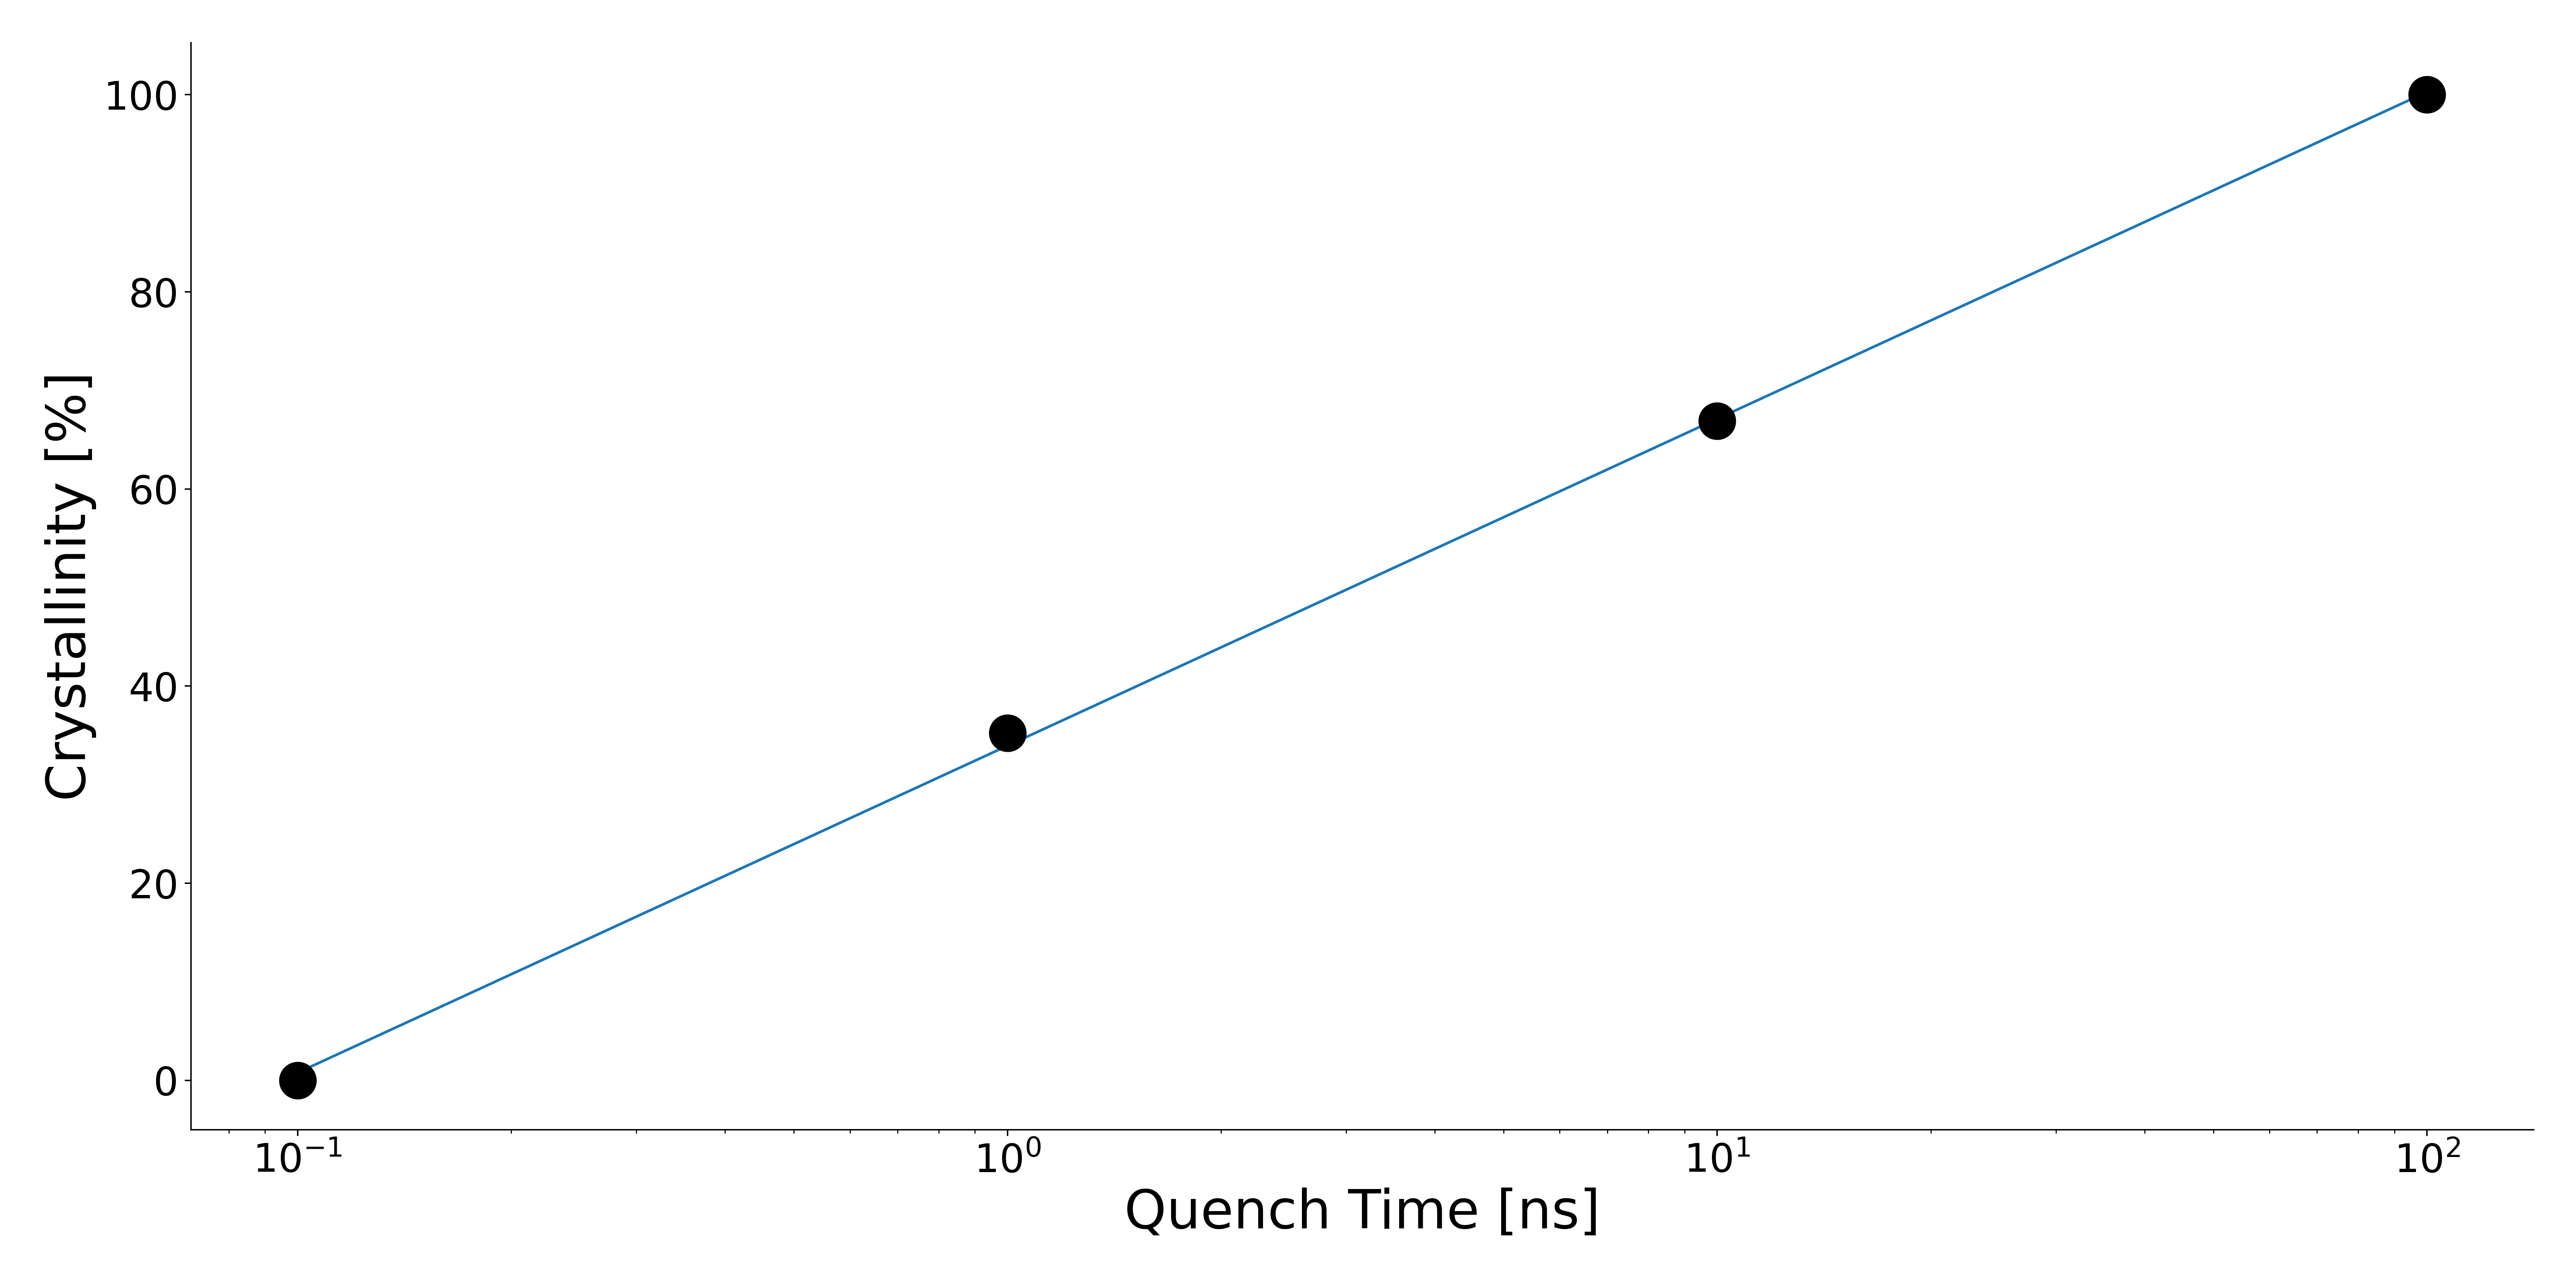
\includegraphics[width=\textwidth]{../img/DifferentQuenchTimes/QuenchTvsCrystallinity.png}
  \caption{\label{fig:crystallinity}The quench time vs crystallinity given by equation \ref{eq:crystallinity}. Black circles show raw data and the dashed black line is a line of best fit using the equation $C = m \ log_{10}(t) + C_{0}$.}
\end{figure}


\chapter{Charge transfer in amorphous systems}
\label{chap:surface_hopping_app}
Although it is important to know the maximum bound on the mobility of the charge carrier in a perfect crystal of an organic semiconductor, in reality it is very difficult to control defect formation in OSs\cite{NGUYEN2006198i, Ray2014}. This is due to van der Waals forces only weakly holding molecules at lattice sites, allowing molecules greater freedom than in traditional inorganic crystal, and increasing the chance of defect formation which can trap/scatter charge carriers reducing overall mobility. This means it is important to investigate and characterise charge transport properties for not just perfectly crystalline OSs but also those that show a range of amorphicity.
\\
\begin{wrapfigure}{r}{0.4\textwidth}
	\vspace*{-0.5cm}
	\includegraphics[width=0.4\textwidth]{img/herringbone.png}
	\caption{An example of the \\herringbone packing \\typically found in \\Pentacene crystals}
	\label{fig:HerringbonePacking}
\end{wrapfigure}
The molecule chosen to investigate amorphous films was pentacene. This molecule is a popular organic semiconductor and the subject of much research due to its high field effect mobility \cite{Hu2005}, use in device applications \cite{Hasegawa_2009} and, more recently, the use of functionalization to alter device properties \cite{Anthony2001, Anthony2002}. The pentacene molecule consists of 5 joined benzene rings (36 atoms) and crystals typically pack with a herringbone motif as shown in figure \ref{fig:HerringbonePacking}.
\clearpage
\section{Creating Amorphous Pentacene}
In order to create the amorphous pentacene systems a melt-quench technique was used. This is a standard technique, often used to create amorphous systems in both computational and experimental  fields \cite{D’Angelo2018, PhysRevB.77.172101, BERBANO201293, KARMWAR201194, KO1996211}. The procedure followed is shown in figure \ref{fig:meltQuenchFlowChart}.
\begin{figure}[H]
	\includegraphics[width=\textwidth]{./img/FlowCharts/MeltQuench.png}
	\caption{\label{fig:meltQuenchFlowChart}The melt-quench scheme used to create amorphous pentacene systems. Blue boxes indicate steps using an NPT ensemble, orange boxes indicate use of a NVT ensemble.}
\end{figure}
\noindent In this procedure, the system was initialised with an individual pentacene molecule on a regular 3D grid using an orthorhombic unit cell. This was chosen to make analysis of the resulting structures easier than with the triclinic unit cell typically used to simulate pentacene crystals. The velocities were initially randomly sampled from a gaussian distribution and a Nose-Hoover thermostat and barostat was used to control the temperature and pressure. The Lammps molecular dynamics package was used \cite{LammpsMain, LammpsURL} and electrostatic interactions were handled with Lammps' particle-particle-particle-mesh ewald method \cite{LammpsPPPME}. RESP \cite{RESP} (restrained electrostatic potential) partial charges were parameterised using Gaussian 16 \cite{g16} with the B3-LYP level of theory and a G-311g(d) basis set. The use of partial charges was essential in the creation of the amorphous systems and will be discussed further in section \ref{sect:partial_charge_importance}. Finally, for inter and intra molecular interactions the general AMBER force-field \cite{GAFF} (GAFF) was applied. There doesn't seem to be one predominant forcefield to use in simulations of pentacene though parameters from GAFF have been used in a number of studies \cite{C0JM01577F, Yoneya2012, PentCrystallisation, MILLER201728, Wang2011, C6CP06436A, doi:10.1246/cl.180450}.
\\\\
Four different quenching times were used spanning 4 orders of magnitude: 0ns, 1ns, 10ns and 100ns. For the 0ns, 1ns and 10ns quenching simulations 3,000 molecules were simulated. In the 100ns quenched structure 3060 molecules were simulated. The initial structure for the 1ns and 10ns quenched structures were taken from a restart of the 0ns quenched simulation after the 800K equilibration step. The 0ns and 1ns quenched structure were carried out under 1 atmosphere of pressure in x, y and z. However, the 10ns quenching required a small increase to 5 atmospheres as the structure had a tendency to deform such that one of the cell vectors became either very large or very small. In the 100ns quenched structure I updated the barostat target pressure (before the phase transition) to account for similar deviations in simulation box dimensions.
\section{Structure of the quenched simulations}
A movie showing the full 100ns melt-quench simulation can be found here: \href{https://youtu.be/6IQcYErQHVs}{https://youtu.be/6IQcYErQHVs}. Still images of the final snapshot of each different quenching time are shown in figure \ref{fig:final_snapshots} below.
\subsection{Final Structure Snapshots}
\noindent We can see qualitatively that as we increase the quenching time from a) $\rightarrow$ d) the structure starts to look more ordered and crystal layers are starting to be formed. Looking longer at the structure we see that lower quench times tend to form small crystal clusters. In the 0ns quenched structure these clusters tend to be just $\sim$7-10 molecules in size. As we increase the quenching time to 1ns we see 1D channels of crystalline pentacene start to form throughout the structure, though the structure is still relatively disordered due to these channels being randomly oriented with respect to one another. As we increase the quenching time these crystal fragments become larger until in the 100ns quenched structure the whole system is comprised of just 2 crystals. The reason for this is, as we decrease the rate of cooling (increase quench time) we also decrease the rate of crystals being seeded. This allows any crystals that have formed to grow larger without being impeded by the growth of any other crystals. This can most clearly be seen in the animation of the \href{https://youtu.be/6IQcYErQHVs}{100ns melt quench simulation} linked above.

\begin{figure}[h]
	\includegraphics[width=\textwidth]{./img/DifferentQuenchTimes/AllTimes.png}
	\caption{\label{fig:final_snapshots}The final snapshot of each quenching simulation visualised in VMD \cite{VMD} and rendered with Tachyon \cite{Tachyon}. Snapshots are ordered by quenching time i.e. a) is the 0ns quench, b) is the 1ns quench and so on.}
\end{figure}
\subsection{Molecular Packing}
We can isolate clusters in each of the different structures shown in figure \ref{fig:final_snapshots} to reveal the molecular packing within. In figure \ref{fig:Layer11} a DBSCAN-like algorithm has been applied to the final structure from the 100ns quench to cluster molecules based on the molecular density in a given region of space. These clusters have then been highlighted by different colours. The top-most green cluster has been rotated such that, on the left, we are viewing it at an angle perpendicular to the plane of molecules, as shown by the cartoon eye. Comparing this plane to the crystal plane to the right of it we can see a remarkable similarity in the packing motif. The herringbone packing has formed and (as can be seen in figure \ref{fig:ang_dist} in section \ref{sect:ang_dist}) the herringbone intersection angle is remarkably similar to the crystal plane. This serves as a confirmation of the choice of force-field and the parameterisation of the partial charges.
\begin{figure}[h]
	\includegraphics[width=\textwidth]{./img/DifferentQuenchTimes/100ns/Layer11_Demonstration.png}
	\caption{\label{fig:Layer11}The 100ns quenched structure with different clusters shown with different colours. A bird's eye view of the green cluster has been shown on the left to demonstrate the herringbone packing within each cluster/layer. The far-right image labelled `Crystal' is a snapshot of a crystal plane after a short MD equilibration.}
\end{figure}
\\\\
\begin{wrapfigure}{r}{0.5\textwidth}
	\centering
	\includegraphics[width=0.51\textwidth]{./img/DifferentQuenchTimes/0ns/Slice6_4Clusters.png}
	\caption{\label{fig:ClustInst}A slice from the 0ns quenched structure with selected clusters of herringbone-like packing highlighted.}
\end{wrapfigure}
Although this herringbone packing pattern is most obvious in the 100ns quenched structure, it can also be seen in the other structures. At the other extreme in the 0ns quenched structure we see small clusters ($<$15 mols) of pentacene crystals forming. This is shown in figure \ref{fig:ClustInst}. As the quench time increases these crystal fragments have more time to grow unimpeded by other crystals seeded nearby.
\\\\
\noindent To quantify the change in the structure for the differently quenched structures 4 macroscopic properties can be plotted: the mass density, the angular distribution, the radial distribution function and the orientational order parameter. These are discussed in the following sections.
\subsection{Mass Density}
The mass density of the 4 different quenching simulations can be seen below in figure \ref{fig:QuenchDensity}. This was calculated by dividing the total mass of the atoms in the system by the volume (product of cell vectors) of the simulation box. The first thing to notice in this graph is as we increase the quenching time we increase the density of the final sample. This is due to the molecules packing more efficiently in the crystal than in an amorphous structure. We also see very clearly in the plots the sudden increase in density associated with the phase transition from liquid to solid Pentacene. In the 1ns quench structure (quenched with the barostat set to 1 atmosphere) this occurs around Pentacene's experimental melting of 530.15K \cite{PentaceneMeltingPoint} providing confirmation of the choice of force-field. The 0ns, 1ns and 10ns runs were performed in a single 24 hour run. The 100ns quench was performed using many restarts, the discontinuities in the density for the 100ns structure come from these restarts. I don't believe they affect the final structure as these only occur while the system is in the liquid state.
\begin{figure}[h]
	\centering
	\includegraphics[width=0.9\textwidth]{./img/DifferentQuenchTimes/Density.png}
	\caption{\label{fig:QuenchDensity}A time series of the density of the quenched structures. The black line shows the experimental mass density of crystal pentacene.}
\end{figure}

\subsection{Angular Distribution}
\label{sect:ang_dist}
The angular distribution shows the distribution angles each molecule makes with the other molecules in the system. In figure \ref{fig:ang_dist} it was calculated by calculating the angle of an axis of each molecule with its nearest neighbours (a 20$\angstrom$ center of mass cutoff was used). This data was then grouped into a histogram which is plotted below.
\begin{figure}[h]
	\includegraphics[width=\textwidth]{./img/DifferentQuenchTimes/AngularDist.png}
	\caption{\label{fig:ang_dist}
\noindent The angular distribution for the 4 different quench times is shown above. The brown and purple lines are from a perfect crystal before and after a short MD run. The others are after the various melt-quench simulations. On the right is a schematic showing which angles are referenced in each plot.}
\end{figure}
In figure \ref{fig:ang_dist} we can see as the quenching time increases we start to notice an ever more prominent peak appear at either extreme of the x axis. This is because the molecules are aligning parallel with one another. The symmetry of the plot is an artefact of the melt stage of the simulation were each molecule was free to rotate randomly.
\\\\
If we now look at the short axis plot we can see that, again, as the quench time increases we start to see a more ordered structure start to form. This time the herringbone intersection angle between molecules (54.3$^{o}$ \cite{PentaceneAngle}) within the herringbone structure is retrieved. This is a result of using partial charges in the simulation -running the same simulations without partial charges results in an unrealistic face-to-face stacking. The brown and purple line show the same calculation run on a crystal of pentacene before and after MD. The purple line comes from an analysis of a repeated unit cell, hence we get 2 delta functions: one at 54.3$^{o}$ and one at 0$^{o}$. This structure was then equilibrated with electrostatics for 50ps and we start to see a broadening of the herringbone intersection angle and to a lesser extent (on the left side) a broadening of the angle between parallel pairs.
\subsection{Radial Distribution Function}
The radial distribution function (RDF) describes the change of density from each particle in the system and is normalised to the bulk density (i.e. $\frac{N}{V}$). This was calculated by counting the number of atoms within a spherical shell from each atom and then dividing by the volume between these spheres. This local density was then normalised to the bulk crystal density. In systems with atoms regularly placed throughout the system we would expect to see sharp peaks in the RDF as there would be many gaps with no atoms. Conversely, with a totally amorphous system we would expect to see (once we reach twice the Van der Waals radius from each atom) a flat line at 1 as local density should be very similar to the global density. This pattern is what we observe in figure \ref{fig:RDF} below. The sharp peaks of the purple line show the RDF of a perfect crystal (repeated unit cell) confirming we have a highly ordered system. On the other extreme the blue line shows very weak ordering of the atoms' positions with any ordering vanishing after $\sim$12.5$\angstrom$ from each atom. This is due to the 0ns structure comprising primarily of small crystal fragments giving rise to a small amount of very local order but over longer distances this order vanishes. Again, as the quench time increases, the ordering increases resulting in larger peaks that more closely match the RDF of the crystal after a short MD equilibration.
\begin{figure}[H]
	\centering
	\includegraphics[width=\textwidth]{./img/DifferentQuenchTimes/RDF.png}
	\caption{\label{fig:RDF}The carbon-carbon radial distribution function for 4 different quenching times and a crystal before and after 50ps of MD. The quenches (0, 1, 10 and 100ns) are shown in blue, orange, green and red respectively. The crystal data are shown in purple and brown.}
\end{figure}

\subsection{Orientational Order Parameter}
The orientational order parameter gives a single number describing how aligned the molecules within a system are. Values lie on a scale from -0.5 to 1, where 1 denotes all molecules are aligned, 0 denotes a random alignment of molecules and -0.5 denotes an anti-alignment with respect to the reference vector. The formula for the orientational order parameter is given below in equation \eqref{eq:OOP}.
\begin{equation}
	S = \frac{3}{2} \ \frac{1}{N_{mol}}\sum_{i}^{N_{mol}} \left[\frac{\mathbf{v}_{i} \cdot \mathbf{v}_{ref}}{|\mathbf{v}_{i}| |\mathbf{v}_{ref}|} \right]^{2}  - \frac{1}{2}
	\label{eq:OOP}
\end{equation}
Where $\mathbf{v}_{i}$ is the vector describing the long or short axis of molecule i. The reference vector $\mathbf{v}_{ref}$ was defined as the average over $\mathbf{v}_{i}$ i.e: $\mathbf{v}_{ref} = \left\langle \mathbf{v}_{i} \right\rangle_{i}$. $N_{mol}$ is the number of molecules and i indicates a molecule index.
\\\\
In figure \ref{fig:OOP} we can see the change in the orientational order parameter with quenching time and, as seen in the previous sections, as we increase the quenching time we increase (orientational) order in the system.
\begin{figure}[h]
	\includegraphics[width=\textwidth]{./img/DifferentQuenchTimes/TimevsOOP.png}
	\caption{\label{fig:OOP}The change in the orientational order parameter (OOP) with respect to the quenching time. The blue data represents the values for the long axis and the orange data represents the short axis values. The horizontal lines show the theoretical value for a perfect crystal.}
\end{figure}

\section{Charge Transfer Properties}
We have seen that the final structure of the pentacene systems becomes more ordered and crystal-like as the quenching time is increased. It would be good now to see how this affects the charge transfer properties. A key quantity governing charge transfer rates is the ratio between electronic coupling and reorganisation energy, $\frac{H_{ab}}{\lambda}$. Seeing as we have a single molecule system, by plotting the electronic coupling we can get a qualitative view of the charge transfer dynamics and see which paths are the most likely within the structure.
\subsection{Coupling Graphs}
In figure \ref{fig:crystalCouplingGraph} the graph of electronic couplings between molecules has been plotted for each of the quenched systems and a crystal system after a short equilibration run with MD. In this figure the centers of mass each molecule is represented by a small black dot and the calculated coupling value with a coloured line (red, green blue). That is, if 2 molecules have a non-negligible coupling between them they would be represented by 2 black dots with either a red, green or blue line connecting them. The couplings were calculated via the analytic overlap method \cite{gajdos_ultrafast_2014} and a pertinent cluster of molecules was selected for each quench time. For the 0ns and 1ns quench times this was simply a slice 1 molecule thick in the z dimension, containing a few hundred molecules. For the 10ns and 100ns quenched structures a reasonable cluster of molecules was chosen after applying a density based clustering algorithm on the superstructure. For the crystal a plane from the crystal was chosen. All panes in figure \ref{fig:crystalCouplingGraph} show the coupling of the selected system from an angle perpendicular to the plane of molecules.
\begin{figure}
	\includegraphics[width=\textwidth]{./img/CouplingPlots/CouplingGraphs_all.png}
	\caption{\label{fig:crystalCouplingGraph}A representative network of electronic coupling that each quenched structure has formed. Each structure is labelled by the quench time (e.g. 0ns, 1ns, 10ns, 100ns) or Crystal for a crystal after a short MD equilibration. Coupling strengths are categorised as high (red), medium (green) and low (blue). The definitions of the categories are given in the legend in the bottom right corner.}
\end{figure}
\\\\
We can see in the graph of the 0ns quenched structure there is very little order to the coupling network. Only very small fragments of high (red) coupling are formed and each one is connected via weak or medium coupling. We can define a 'high coupling fragment' as any set of molecules which can all be reached from any member of the set via an unbroken path of high coupling. The mean size of these high coupling fragments in the 0ns structure is 4.1 molecules and there are 503 of them. In this structure we would expect to see a localised polaron (over a $\sim$ 3 molecules) and low mobilities due to the lack of conductive channels in the structure. The mean size of fragments increases and the number of fragments decreases as we increase the quenching time as shown in table \ref{tab:cluster_sizes}.
\\
\begin{table}[h]
	\begin{tabular}{cccc}
		\textbf{Quench Time} [ns] & \textbf{Mean Fragment Size} & \textbf{Fragment Size Std Dev} & \textbf{Num Fragments} \\
		\hline &&&\\
		0 & 4.2 & 3.8 & 503 \\
		1 & 4.5 & 5.0 & 493 \\
		10 & 6.5 & 9.3 & 373 \\
		100 & 8.7 & 16.2 & 292 \\
		\hline &&&\\
	\end{tabular}
	\caption{\label{tab:cluster_sizes}The change in the number of high coupling fragments, and the mean and standard deviation of their size, found in each structure as the quenching time was varied.}
\end{table}
\\
We can see in table \ref{tab:cluster_sizes} that as the quenching time increases, the size of the highly coupled fragments (how many molecules are connected) increases and fewer of them are formed. The standard deviation also increases showing in the 0ns quenched structure most fragments are very small but as we increase the quench time we still get smaller fragments but much larger ones can now form too. These larger fragments can act as regions of high conductivity allowing much larger mobilities to be achieved than in the quicker quenching times.

\clearpage
\subsection{Molecular Dynamics without Partial Charges}


\label{sect:partial_charge_importance}


\chapter{Extending surface hopping}
\label{chap:surface_hopping_ES}

\noindent FOB-SH is a variant of Tully's original fewest switches surface hopping \cite{FSSH_orig}. It has been used to simulate electron-nuclear dynamics in large systems of organic molecules and has been well tested against experimental studies and benchmarked against higher order studies \cite{FlickPolarons, Giannini2018Crossover, Giannini2019,             C9TC05270D, Carof2017FSSH, C9FD00046A, C9CP04770K, FOB-SH_Spencer,        C6FD00107F}. However, the code does not currently account for any electrostatic interactions. This presents a problem when looking at many systems; such as those with large amounts of disorder or those with polariseable molecules. 
%Need more motivation of implementing electrostatics in CP2K
\\\\
The standard Coulomb sum of partial charges is only conditionally convergent and extremely slow to calculate. The standard method for calculating electrostatic interactions is by decomposing interactions into long-range and short-range interactions (with corrections such as removing bonded terms etc\ldots). This is normally carried out with an Ewald sum \cite{Ewald} where a short-range interactions are calculated in real space and long-range interactions are calculated in reciprocal space. This results in 2 summations that are now unconditionally, quickly convergent. Further extensions to the standard Ewald technique provide an additional decrease in computational time by interpolating particles onto a grid and using fast fourier transforms to calculate all interactions. Although fast and formally exact, the Ewald sum has some major drawbacks in that it assumes a 3D periodicity and is often one of the most expensive parts of a molecular dynamics simulation \cite{EwaldReview}. In Wolf, 99 \cite{Wolf99}, a technique for removing the (expensive) reciprocal space term from the sum altogether was proposed by ensuring charge neutrality within a cutoff sphere from each atom. The idea was inspired from an observation that: if the net sum of charges within the cutoff sphere was 0 then the standard coulomb sum seemed to converge well on accurate Madelung energies. This idea was developed to improve energy conservation and to remove discontinuities within the forces and energies \cite{Zahn2002, DSF}. In this work I will investigate the applicability of both the standard Ewald technique and a development of the Wolf method (named DSF \cite{DSF}) to calculate the electrostatic interactions within FOB-SH.
\section{Implementation details -addition subtraction method}
\label{sect:addSubMethod}
\begin{figure}[ht]
  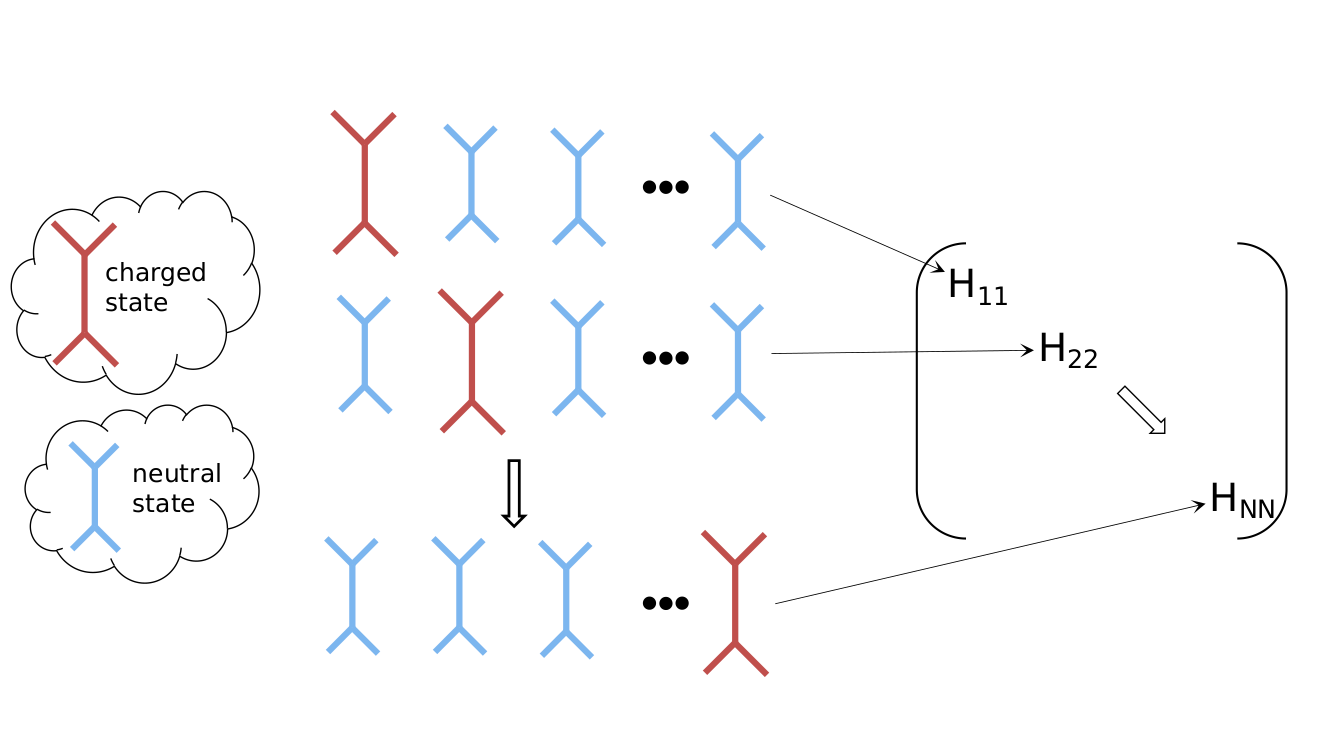
\includegraphics[width=\textwidth]{./img/ES/ForceEnerCalc.png}
  \caption{\label{fig:FE_Calc}A demonstration of the procedure to calculate diagonal elements of the Hamiltonian (site-energies). Red (blue) shapes represent a molecule in its charged (neutral) state. A  horizontal line of these shapes represent the full system with all molecules; where a single molecule is in its charged state. The arrow denotes which matrix element this saved as.}
\end{figure}
\noindent In FOB-SH, nuclear dynamics are determined by the Hamiltonian. The Hamiltonian is constructed such that the diagonal elements (site-energies) come from a classical forcefield and the off-diagonal elements (electron couplings) are proportional to the overlap of the diabatic wavefunctions. Each site-energy, $H_{\gamma \gamma}$, is defined as the potential energy of the system where the excess charge is localised on the molecule $\gamma$. For the avoidance of doubt, I will denote the molecule with the excess charge localised on it as the `charged' molecule and other molecules as `neutral'. The presence of the excess charge on molecule $\gamma$ results in different input parameters (such as the charge distribution or the length of bonds) than the other neutral molecules. This results in the calculation of site-energies and forces having to be repeated $N_{mol}$ times for each permutation of the charged molecule. This is summarised in figure \ref{fig:FE_Calc}. 
\\\\
To determine whether it is feasible to repeat the calculation of the electrostatic interactions $N_{mol}$ times a quick timing run was carried out. This simulated 250 pentacene molecules (9,000 atoms) and the time was measured to calculate the electrostatic interactions with the 3 methods already implemented within CP2K: Smooth Particle Mesh Ewald (SPME), Particle Mesh Ewald (PME) and standard Ewald. The measured time of a simulation without any electrostatics was then subtracted from each of these simulations to isolate the time spent on just the electrostatics. The results are given in figure  \ref{fig:ES_Timings}.
\begin{figure}[ht]
  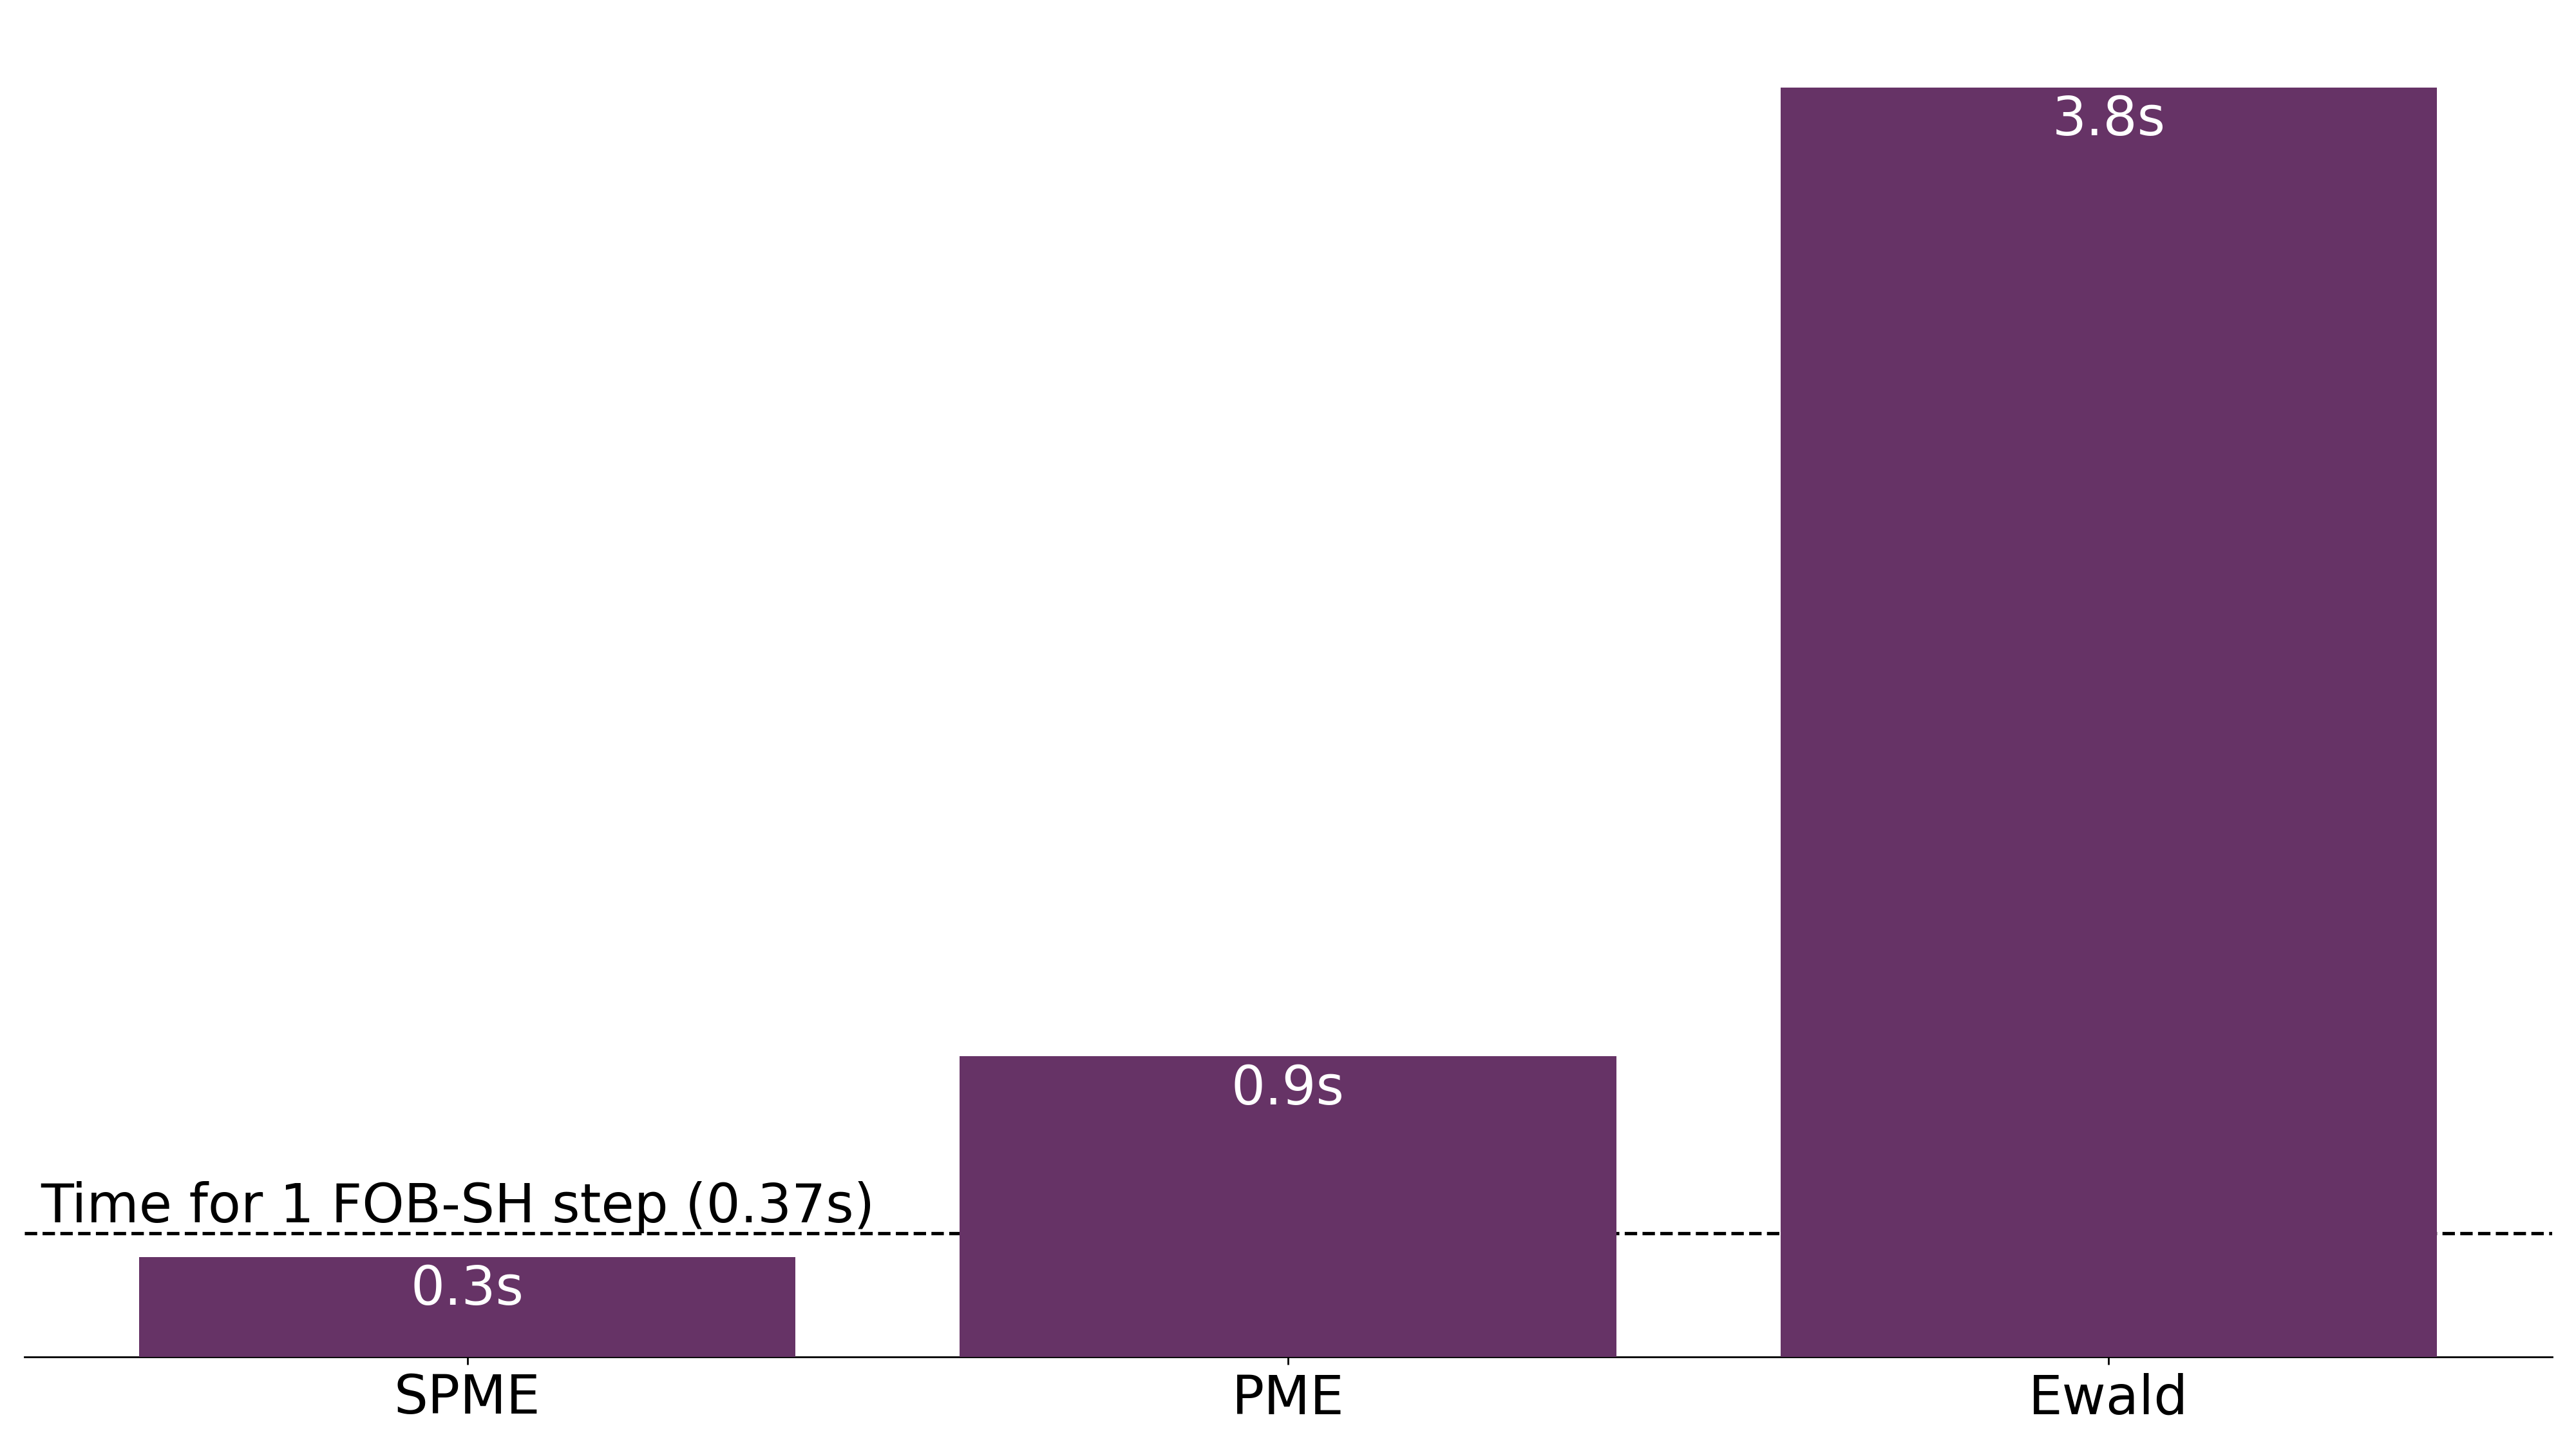
\includegraphics[width=\textwidth]{./img/ES/InitialTimings.png}
  \caption{\label{fig:ES_Timings}The time taken to calculate just the electrostatic interactions within CP2K for a 9,000 atom system using various methods. PME is particle mesh Ewald, SPME is smooth-PME, Ewald is the standard ewald method. The dashed line shows the time taken for a single FOB-SH step.}
\end{figure}
\\
We can see that even a single calculation of the electrostatic interactions with the fastest method available within CP2K (SPME) will take a length of time comparable to the rest of the surface hopping code. It is clear then that a more efficient method must be used to calculate the electrostatics.
\\
\begin{figure}[ht]
  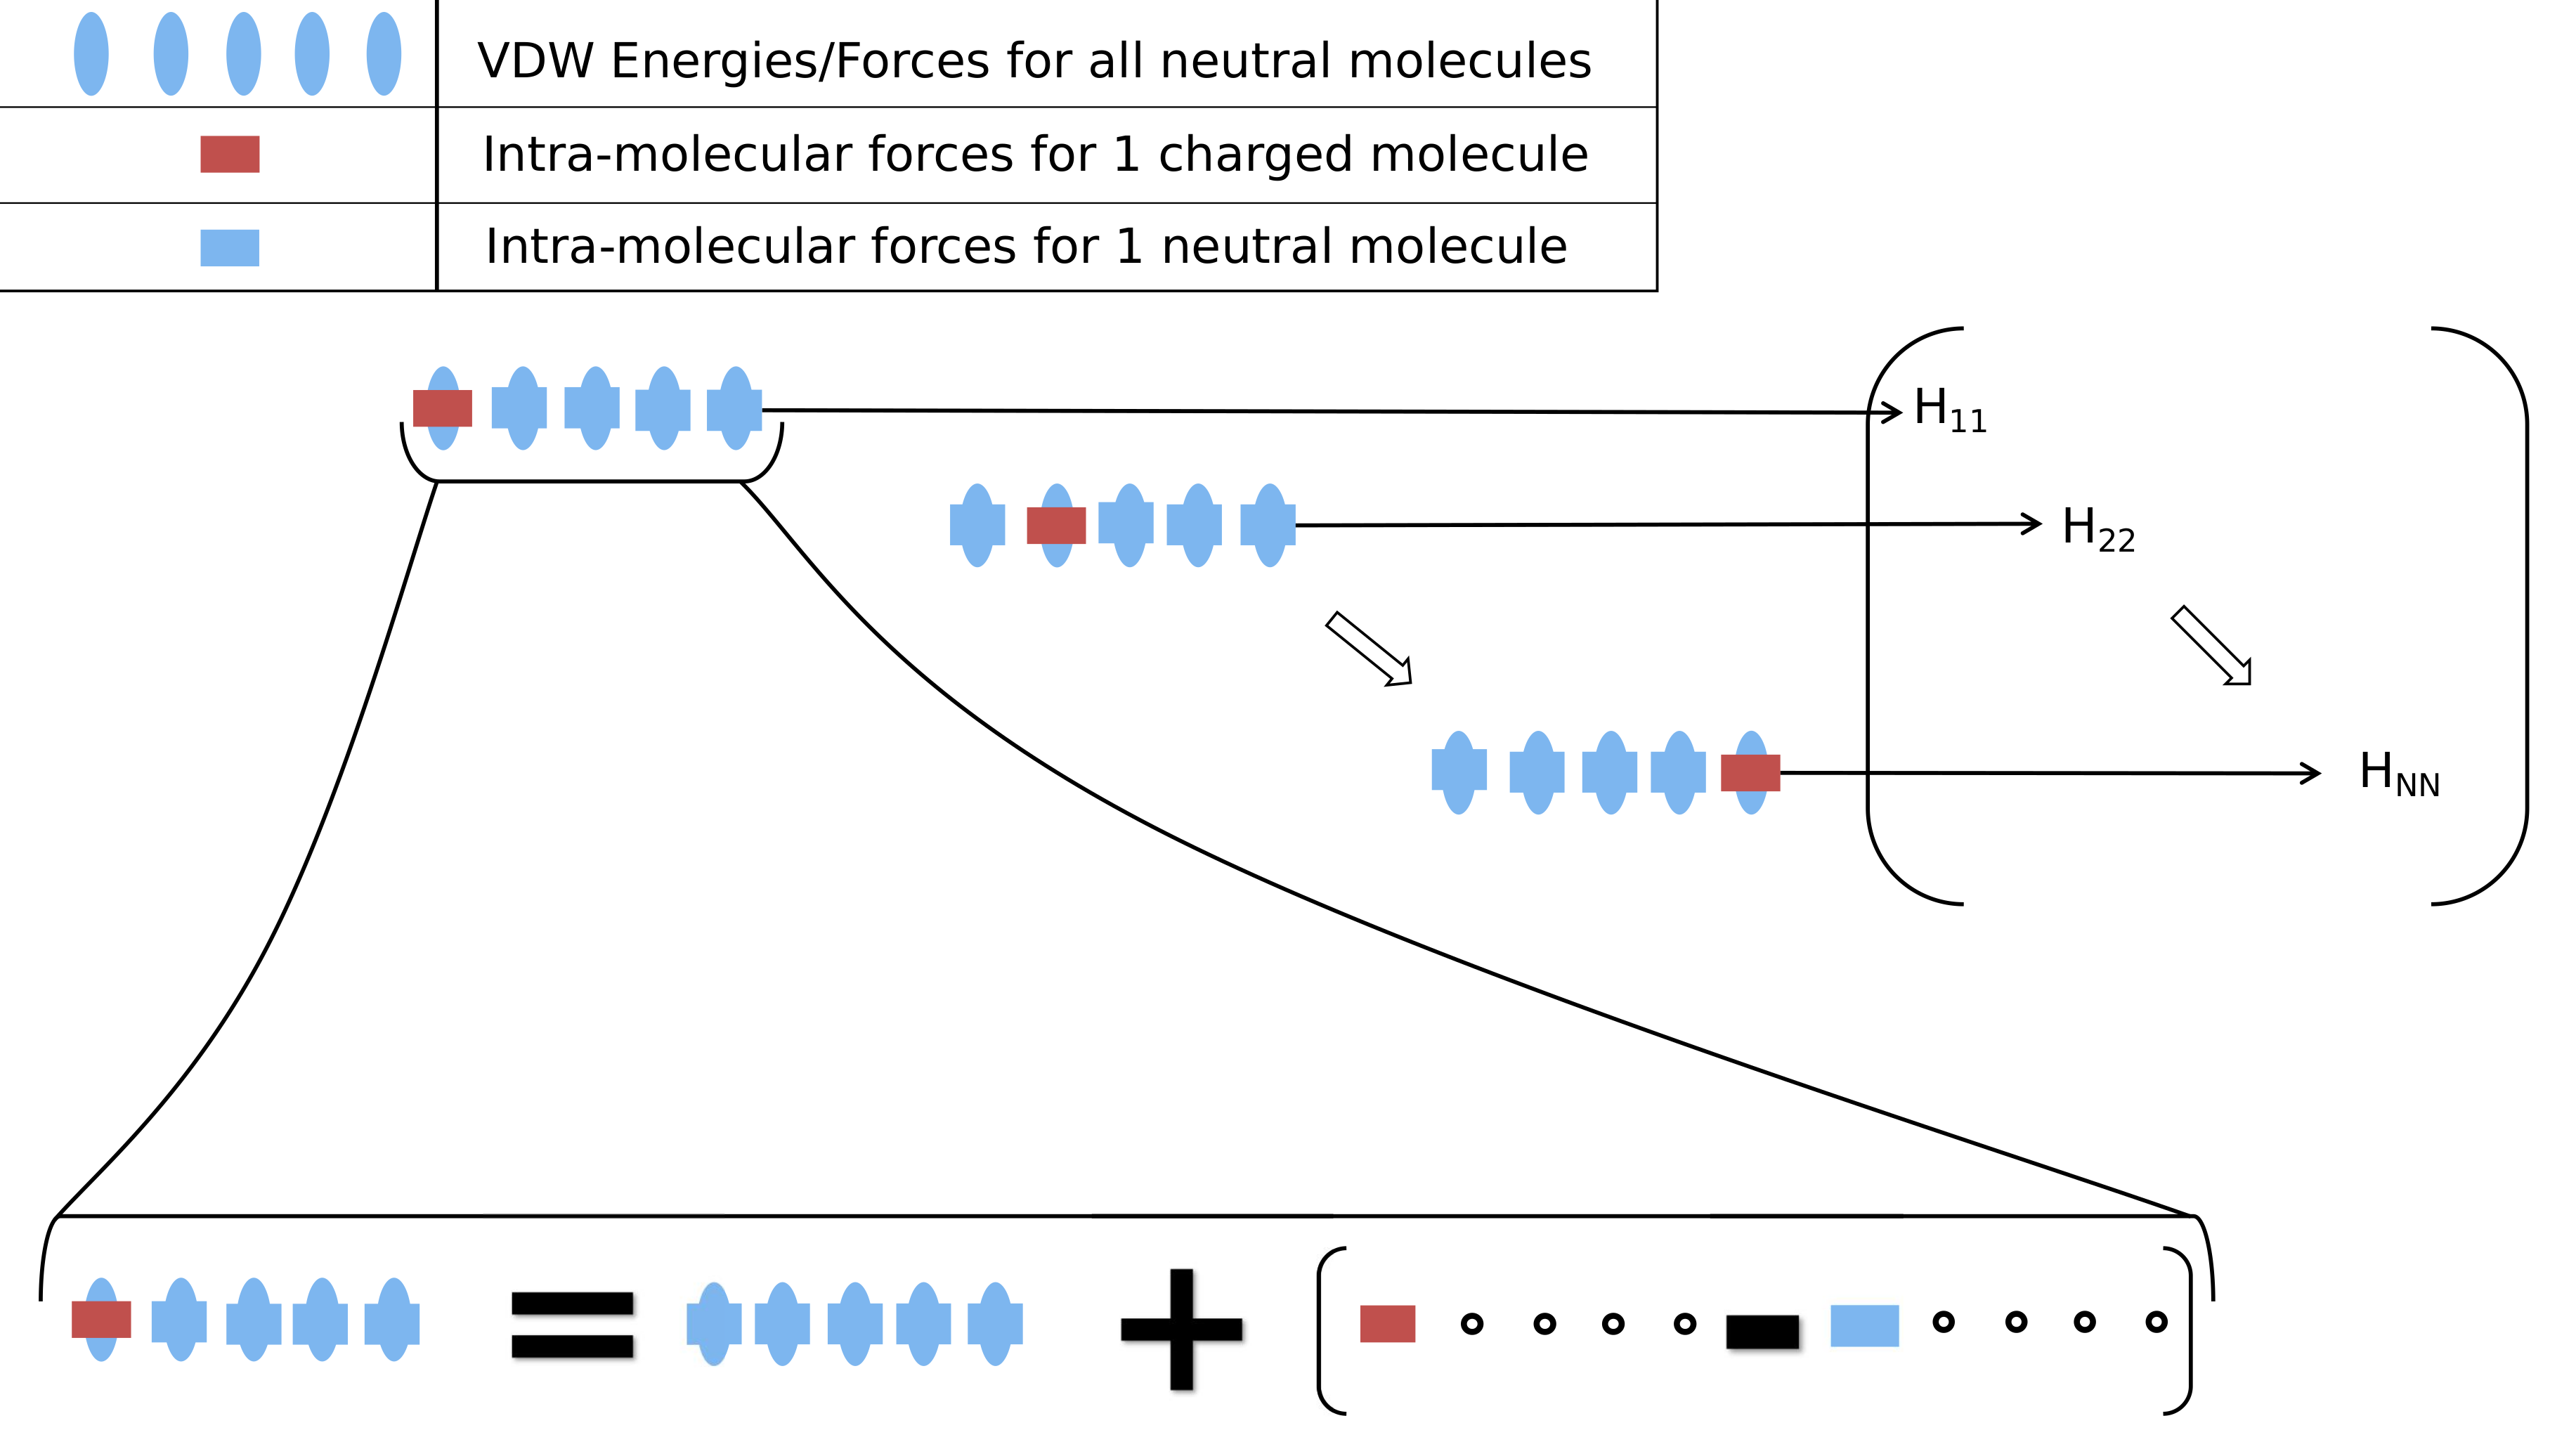
\includegraphics[width=\textwidth]{./img/ES/ForceEnerDecomp.png}
  \caption{\label{fig:enerF_decomp}A depiction of the decomposition of the forces and energies within FOB-SH. First the all neutral VDW forces/energies are computed (blue ovals). Second the intra-molecular forces for each charged (neutral) molecule, represented by a red (blue) rectangle. The site-energy/force is then computed as a summation of all molecules in their neutral state with a molecule in its neutral state subtracted and the same molecule in its charged state added.} 
\end{figure}
\\
Within the current FOB-SH implementation the forces and energies consist of intra-molecular components (bonds, bends, torsions etc\ldots) and inter-molecular components (Van der Waals forces provided by a Leonard-Jones potential). The same repetition of the calculation of forces and energies would, at first glance, be required for the correct calculation of these terms. However, an addition-subtraction scheme is used to reduce the calculation time from $O(N_{mol}, N_{atom}^2)$ to $O(N_{atom}^2)$. This is summarised in figure \ref{fig:enerF_decomp} and relies on the fact that the intra-molecular forces and energies can be decomposed into independent molecular contributions. In order to calculate the force on each atom and site-energy with molecule $\gamma$ in its charged state the code first calculates the force/energy with all molecules in their neutral state and then adds the contribution of molecule $\gamma$ in its charged state and subtracts the contribution of molecule $\gamma$ in its neutral state. We do not make the same adjustment for the VDW forces as the correction is negligible. This results in just 2 calculations of all forces and total energies rather than $O(N_{mol})$ calculations. This scheme can be used because the intra-molecular forces can be naturally decomposed into discrete molecular contributions. That is, the calculation of the intra-molecular interactions are decoupled from their environment are independent of the charge state of all other molecules. The electrostatic interactions are, unfortunately, not so intuitively broken down. However, a similar trick can be used to reduce the cost of the Ewald sum. In the following work, I will present 2 frameworks in which to calculate electrostatic interactions -the recalculation method and the addition-subtraction method. The recalculation method references the method of na\"ively looping over all molecules and recalculating energies and forces without optimisations. This would involve recalculating all interactions for every permutation of charged/neutral molecules. The addition-subtraction scheme is explained in the proceeding chapters.
\subsection{Ewald Equations and the additional subtraction scheme}
The standard Ewald summation for evaluating electrostatic energies in molecular dynamics simulation are given below:
\begin{align}
  \begin{split}
E_{coul}\left(\mathbf{r}\right)
=
% Real Space Sum
\frac{1}{2}\frac{1}{4 \pi \epsilon_0} \sum_{\mathbf{n}} \sum_{j}^{N_{at}} \sum_{i}^{N_{at}} q_i q_j \frac{erfc\left( \alpha \cdot |\mathbf{r}_{ij} + \mathbf{n}|\right)}{|\mathbf{r}_{ij} + \mathbf{n}|} \Theta\left( r_{cut} - |\mathbf{r}_{ij} + \mathbf{n}| \right)
\\
% Reciprocal Space Sum
+
\frac{1}{2\pi V} \ \frac{1}{4 \pi \epsilon_0} \sum_{\mathbf{k} \neq 0} \frac{1}{|\mathbf{k}|^2} e^{-\frac{\pi^2 \ |\mathbf{k}|^2}{\alpha^2}} \ \left|\sum_{j}^{N_{at}} q_{j} e^{2\pi i \mathbf{k} \cdot \mathbf{R}_{j}}\right|^2 \\
% Self Term
- \frac{\alpha}{\sqrt{\pi}} \frac{1}{4 \pi \epsilon_{0}} \sum_{j} q_{j}^2
\\
% Bonded Correction Term
- \frac{1}{2} \frac{1}{4 \pi \epsilon_0} \sum_{j}^{N_{at}} \sum_{i}^{N_{at}} q_i q_j \frac{erfc\left( \alpha \cdot |\mathbf{r}_{ij}|\right)}{|\mathbf{r}_{ij}|} \Theta\left( r_{cut} - |\mathbf{r}_{ij}| \right) 
	\end{split}
\label{eq:EwaldStd}
\end{align}
In equation \eqref{eq:EwaldStd}, the first term is the real space sum. This sums over all periodic images ($\mathbf{n}$) and pairs of atoms $i$, $j$ within a cutoff imposed by the Heaviside step function $\Theta(r_{cut} - |\mathbf{r}_{ij}+\mathbf{n}|)$. The distance between atoms is given by $\mathbf{r}_{ij} = \mathbf{r}_{i} - \mathbf{r}_{j}$, the charge on atom $i$ is given by $q_{i}$ and alpha is a convergence parameter. The factor $\frac{1}{2}$ accounts for any double counting of atoms. The second term is the most expensive part of this calculation and sums over reciprocal space vectors $\mathbf{k}$ and atoms, $j$. $\mathbf{R}_{j}$ represents the position vector of atom $j$. The third term is the constant self-energy term and the fourth corrects for bonded  (intra-molecular) interactions. The bonded interactions may be ignored in the real space sum, this correction removes their effect from the reciprocal space sum. As these 4 summations are independent we can look at each one separately when implementing the addition-subtraction scheme, starting with the simplest -the self-energy term. Note in this section I will only discuss the energies, the forces are very similar and their equations are given in appendix \ref{ap:EwaldForcesAddSub}.
\subsection{Self-energy addition subtraction scheme}
The self energy term is a correction for over counting within the reciprocal space sum. For each site-energy, $\gamma$, we must recalculate the full forces and energies with the excess charge located on molecule $\gamma$. This is demonstrated in equation \eqref{eq:SelfNoScheme}. Note that for brevity I have replaced the factor $\frac{1}{4 \pi \epsilon_0}$ with $\eta$.
\begin{equation}
  E_{self}^{\gamma} = \frac{\alpha}{\sqrt{\pi}} \eta \left[\sum_{j \not\in \gamma} \left(q^{n}_{j}\right)^2  + \sum_{j \in \gamma} \left(q^{c}_{j}\right)^2\right]
  \label{eq:SelfNoScheme}
\end{equation}
In the above equation, the Ewald self-energy correction contribution for site-energy $\gamma$ is simply a sum of squared neutral charges for atoms belonging to molecules that aren't $\gamma$ plus the sum of squared charged charges of atoms within $\gamma$. For clarity, the terms `neutral charges' and `charged charges' refer to charges with molecules parameterised in their neutral (no excess charge carrier) and charged (excess charge carrier localised on the molecule) state. This is represented by the superscript $n$ and $c$ where $q^{n}_{j}$ represents the charge on atom $j$ where the force-field for the molecule it belongs to has been parameterised in its neutral state. $q^{c}_{j}$ represents the charge on atom $j$, where the force-field for the molecule the atom belongs to has been parameterised in its charged state.
\\\\
For a single molecule system this value is the same for all $\gamma$ and no optimisations are required, except to calculate this value once and use it for each $\gamma$. However, for a more complex system the addition subtraction scheme used is given in equation \eqref{eq:SelfScheme}.
\begin{equation}
  E_{self}^{\gamma} = \eta \underbrace{\frac{\alpha}{\sqrt{\pi}} \sum_{j}^{N_{at}}\left(q_{j}^{n}\right)^2}_{\text{Calculated Once}} + \underbrace{\frac{\alpha}{\sqrt{\pi}} \eta \sum_{j \in \gamma} \left[ (q^{c}_{j})^2 - (q^{n}_{j})^2 \right]}_{\text{Calculated for each $\gamma$}}
  \label{eq:SelfScheme}
\end{equation}
In equation \eqref{eq:SelfScheme} we have removed the $\gamma$ index from the most expensive part of the sum; this means we can calculate it once and store it. In the second term we only sum over atoms in charged molecule $\gamma$ and remove the contribution from molecule $\gamma$ in its neutral state and add the contribution from molecule $\gamma$ in its charged state. Seeing as the correction part of equation \eqref{eq:SelfScheme} is the only part repeated from each $\gamma$ this reduces the cost of this calculation from $O(N_{mol}, N_{atom})$ to just $O(N_{atom})$. The same idea is used for the remaining terms in the Ewald sum.
\subsection{real space addition subtraction}
The real space term is more complicated than the self-energy term, though the idea is the same. That is, the fully neutral contribution is calculated and for individual sites/molecules a correction is applied. This is shown in equation \eqref{eq:RealScheme}
\begin{align}
  \begin{split}
	  E^{\gamma}_{real} &= \frac{\eta}{2} \sum_{\mathbf{n}} \sum_{j}^{N_{at}} \sum_{i}^{N_{at}} q^{n}_i q^{n}_j  \ R^{dir}(|\mathbf{r}_{ij} + \mathbf{n}|) \\
	  &+ \frac{\eta}{2} \sum_{\mathbf{n}} \sum_{j \in \gamma, i \in \gamma} (q_j^c q_i^c - q_j^n q_i^n) \ R^{dir}(|\mathbf{r}_{ij} + \mathbf{n}|) \\
	  &+ \frac{\eta}{2} \sum_{\mathbf{n}} \sum_{j \in \gamma, i \not\in \gamma} (q_j^c - q_j^n)q_i^n \ R^{dir}(|\mathbf{r}_{ij} + \mathbf{n}|) 
  \end{split}
  \label{eq:RealScheme}
\end{align}
In equation \eqref{eq:RealScheme} the most expensive summation ($O(N_{atom}^2)$) is the first term. Fortunately, we can once again calculate this once and use the same value for each site-energy. This first term calculates all interactions between atoms belonging to molecules in their neutral state (neutral-neutral interactions). The next two terms show the addition-subtraction correction. The second term shows a sum over all pairs of atoms in the charged molecule, $\gamma$. In this term we subtract any neutral-neutral interactions and replace them with any charged-charged interactions. This scales as $O(N_{\text{atom per mol}})$ and is repeated $N_{mol}$ times so the full correction scales as $O(N_{atom})$. The third term replaces any interactions of atoms on the charged molecule with its environment (neutral molecules), hence it removes neutral-neutral interactions and replaces them with charged-neutral interactions. This scales as $O(N_{\text{atom per mol}}, N_{atom})$ and is repeated $N_{mol}$ times, resulting in an ultimate scaling of $O(N_{atom}^2)$. Therefore, this optimisation scales in the same manner as a single calculation of the Ewald interactions and any additional overheads will be minimal. For the avoidance of doubt, in equation \eqref{eq:RealScheme} I have replaced the complementary error function and Heaviside step function in equation \eqref{eq:EwaldStd} with the term $R^{dir}(\mathbf{r}_{ij} + \mathbf{n})$.
\subsection{Bonded corrections addition subtraction}
The bonded correction terms remove electrostatic contributions to energies (and forces) for atoms that are bonded. This is because interactions are already accounted for by the intra-molecular force-field (bonds, bends, torsions etc\ldots). These interactions are easily removed from the real space sum by omitting them in the loop. Therefore, this is a correction only for the reciprocal space sum.
\\\\
These interactions occur within molecules and their contribution can be decomposed into molecular contributions. These interactions can therefore be handled in the same way as the intra-molecular addition-subtraction scheme as discussed in section \ref{sect:addSubMethod}.
\subsection{reciprocal space addition subtraction}
The reciprocal energies can be optimised using the addition-subtraction technique. However, the forces cannot. This is a big problem for any implementation of Ewald electrostatics within surface hopping as the electrostatic part of the Ewald sum is by far the most expensive. In fact in the same 250 molecule system as in figure \ref{fig:ES_Timings} the reciprocal space component took 88\% of the calculation time. In larger systems this increases. Repeating this calculation $N_{mol}$ times would be far too slow and would limit the surface hopping code to small systems of tens of molecules. However, the damped shifted forces technique (DSF) \cite{DSF} can be used to approximate the electrostatic interactions without the reciprocal force term. For completeness I have included the addition-subtraction scheme for the reciprocal space energies below in equation \eqref{eq:RecipScheme} and for the forces in appendix \ref{ap:EwaldForcesAddSubRecip}.
\begin{equation}
  E^{\gamma}_{recip} = \frac{1}{2 \pi V} \sum_{\mathbf{k} \neq 0} \frac{1}{|\mathbf{k}|^2} e^{\frac{\pi^2 |\mathbf{k}|^2}{\eta^2}} \left| \sum_{j}^{N_{at}} q^{n}_{j} e^{2 \pi \mathbf{k} \cdot \mathbf{R}_{j}}  + \sum_{j \in \gamma}^{N_{at}} (q^{c}_{j} - q^n_j) e^{2 \pi \mathbf{k} \cdot \mathbf{R}_{j}} \right| ^2
  \label{eq:RecipScheme}
\end{equation}
Once again in equation \eqref{eq:RecipScheme} the summation over all atoms can be calculated once and reused for each site-energy $\gamma$. This calculates all neutral-neutral interactions. The additional sum over atoms belonging to molecule $\gamma$ is then repeated $N_{mol}$ times for each site-energy $\gamma$.
\section{Timing the electrostatics implementation}
\begin{figure}[ht]
  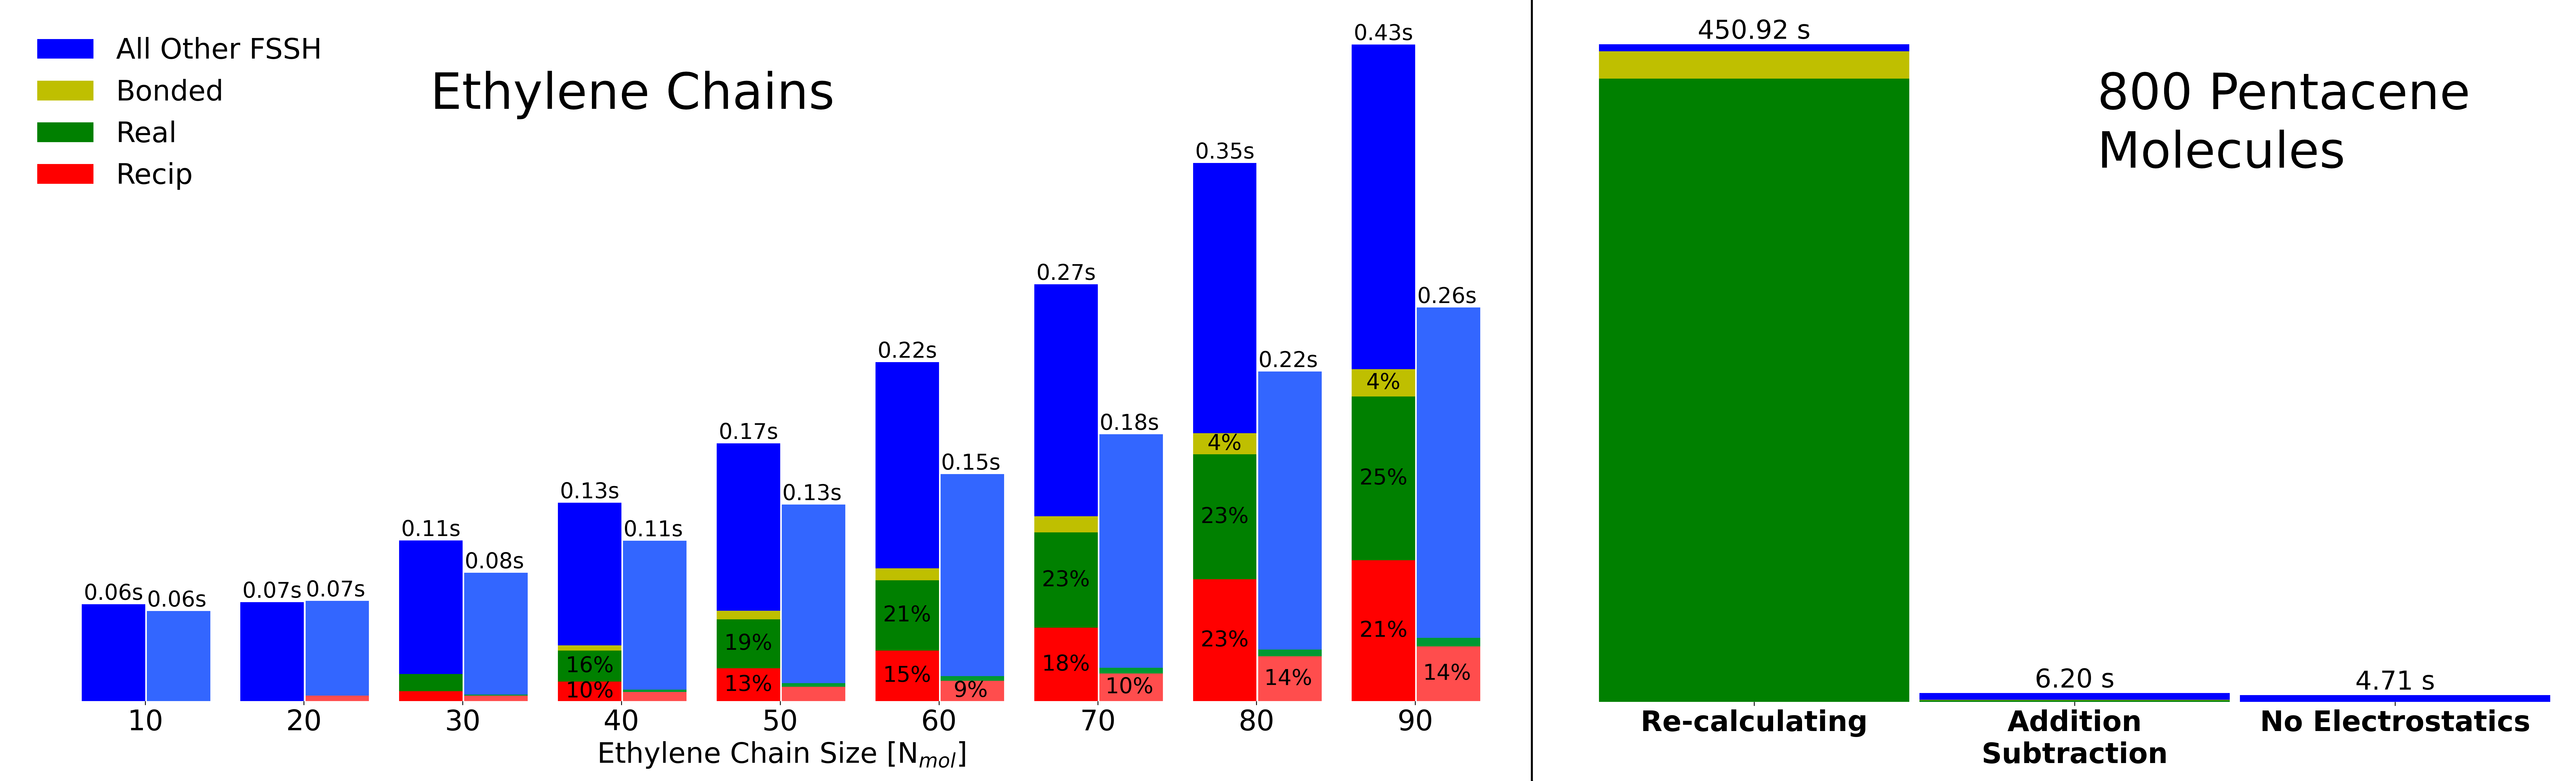
\includegraphics[width=\textwidth]{./img/ES/TimingsReCalc_vs_AddSub.png}
  \caption{\label{fig:AddSubTimings}Time taken to run surface hopping and electrostatics for various lengths of 1D ethylene chain (left) and 800 molecule pentacene plane (right). Darker colors show data from the recalculation method for the electrostatics and less saturated colors to the right show data from the addition subtraction scheme. Green bars show the time taken to calculate real space interactions, red is reciprocal, yellow is the bonded corrections and blue shows all other parts of the surface hopping code. In the right pane reciprocal interactions are omitted as they took too long to run.}
\end{figure}
\noindent In figure \ref{fig:AddSubTimings} the time taken for a single step of a surface hopping simulation for various lengths of a 1D ethylene chain can be seen (left panel). We see as the chain size increases it becomes more important that electrostatic interactions are efficiently handled. In fact for just a 90 molecule ethylene chain calculating the electrostatics takes longer than all other parts of surface hopping. On the right of the same figure, timings for a 800 molecule pentacene plane are shown. In these simulations, the reciprocal calculations took far too long and had to be turned off to measure the time taken for the other components. In this panel we see the significant speed-up for larger system sizes when using the addition-subtraction scheme. However, even with the addition-subtraction scheme the full reciprocal space calculations still take far too long. This is because the calculation of the forces are still repeated $N_{mol}$ times as they cannot be optimised in the same way. A small speedup is seen due to the addition-subtraction scheme being used with the reciprocal space energies. However, we see that the addition-subtraction scheme offers a major speedup for all other components. It is, of course, also vital that the results outputted are correct. I have tested both the recalculation method and the addition-subtraction method against standard CP2K calculations to ensure the implementation is correct. In the following section I will present results only for the addition-subtraction scheme. Although, the re-calculation method was tested in the same way.

\subsection{Testing the electrostatics implementation}
\label{sect:testESimp}
To test the calculation of site-energies and forces within CP2K a 10 molecule ethylene chain was used. In order to produce reference data the new implementation could be checked against, classical MD in CP2K was used to calculate the site-energies and forces for 10 different system. In each one of these simulations a different molecule was chosen to have charged geometry and the rest were chosen to have neutral geometry in the input files. A single step of MD was then carried out and forces and energies were outputted. These forces and energies were subsequently compared to the forces and energies outputted by the both the recalculation and addition-subtraction method. The results for the tests of the addition-subtraction method are shown in figure \ref{fig:AddSubEwaldTest}.
\begin{figure}[ht]
  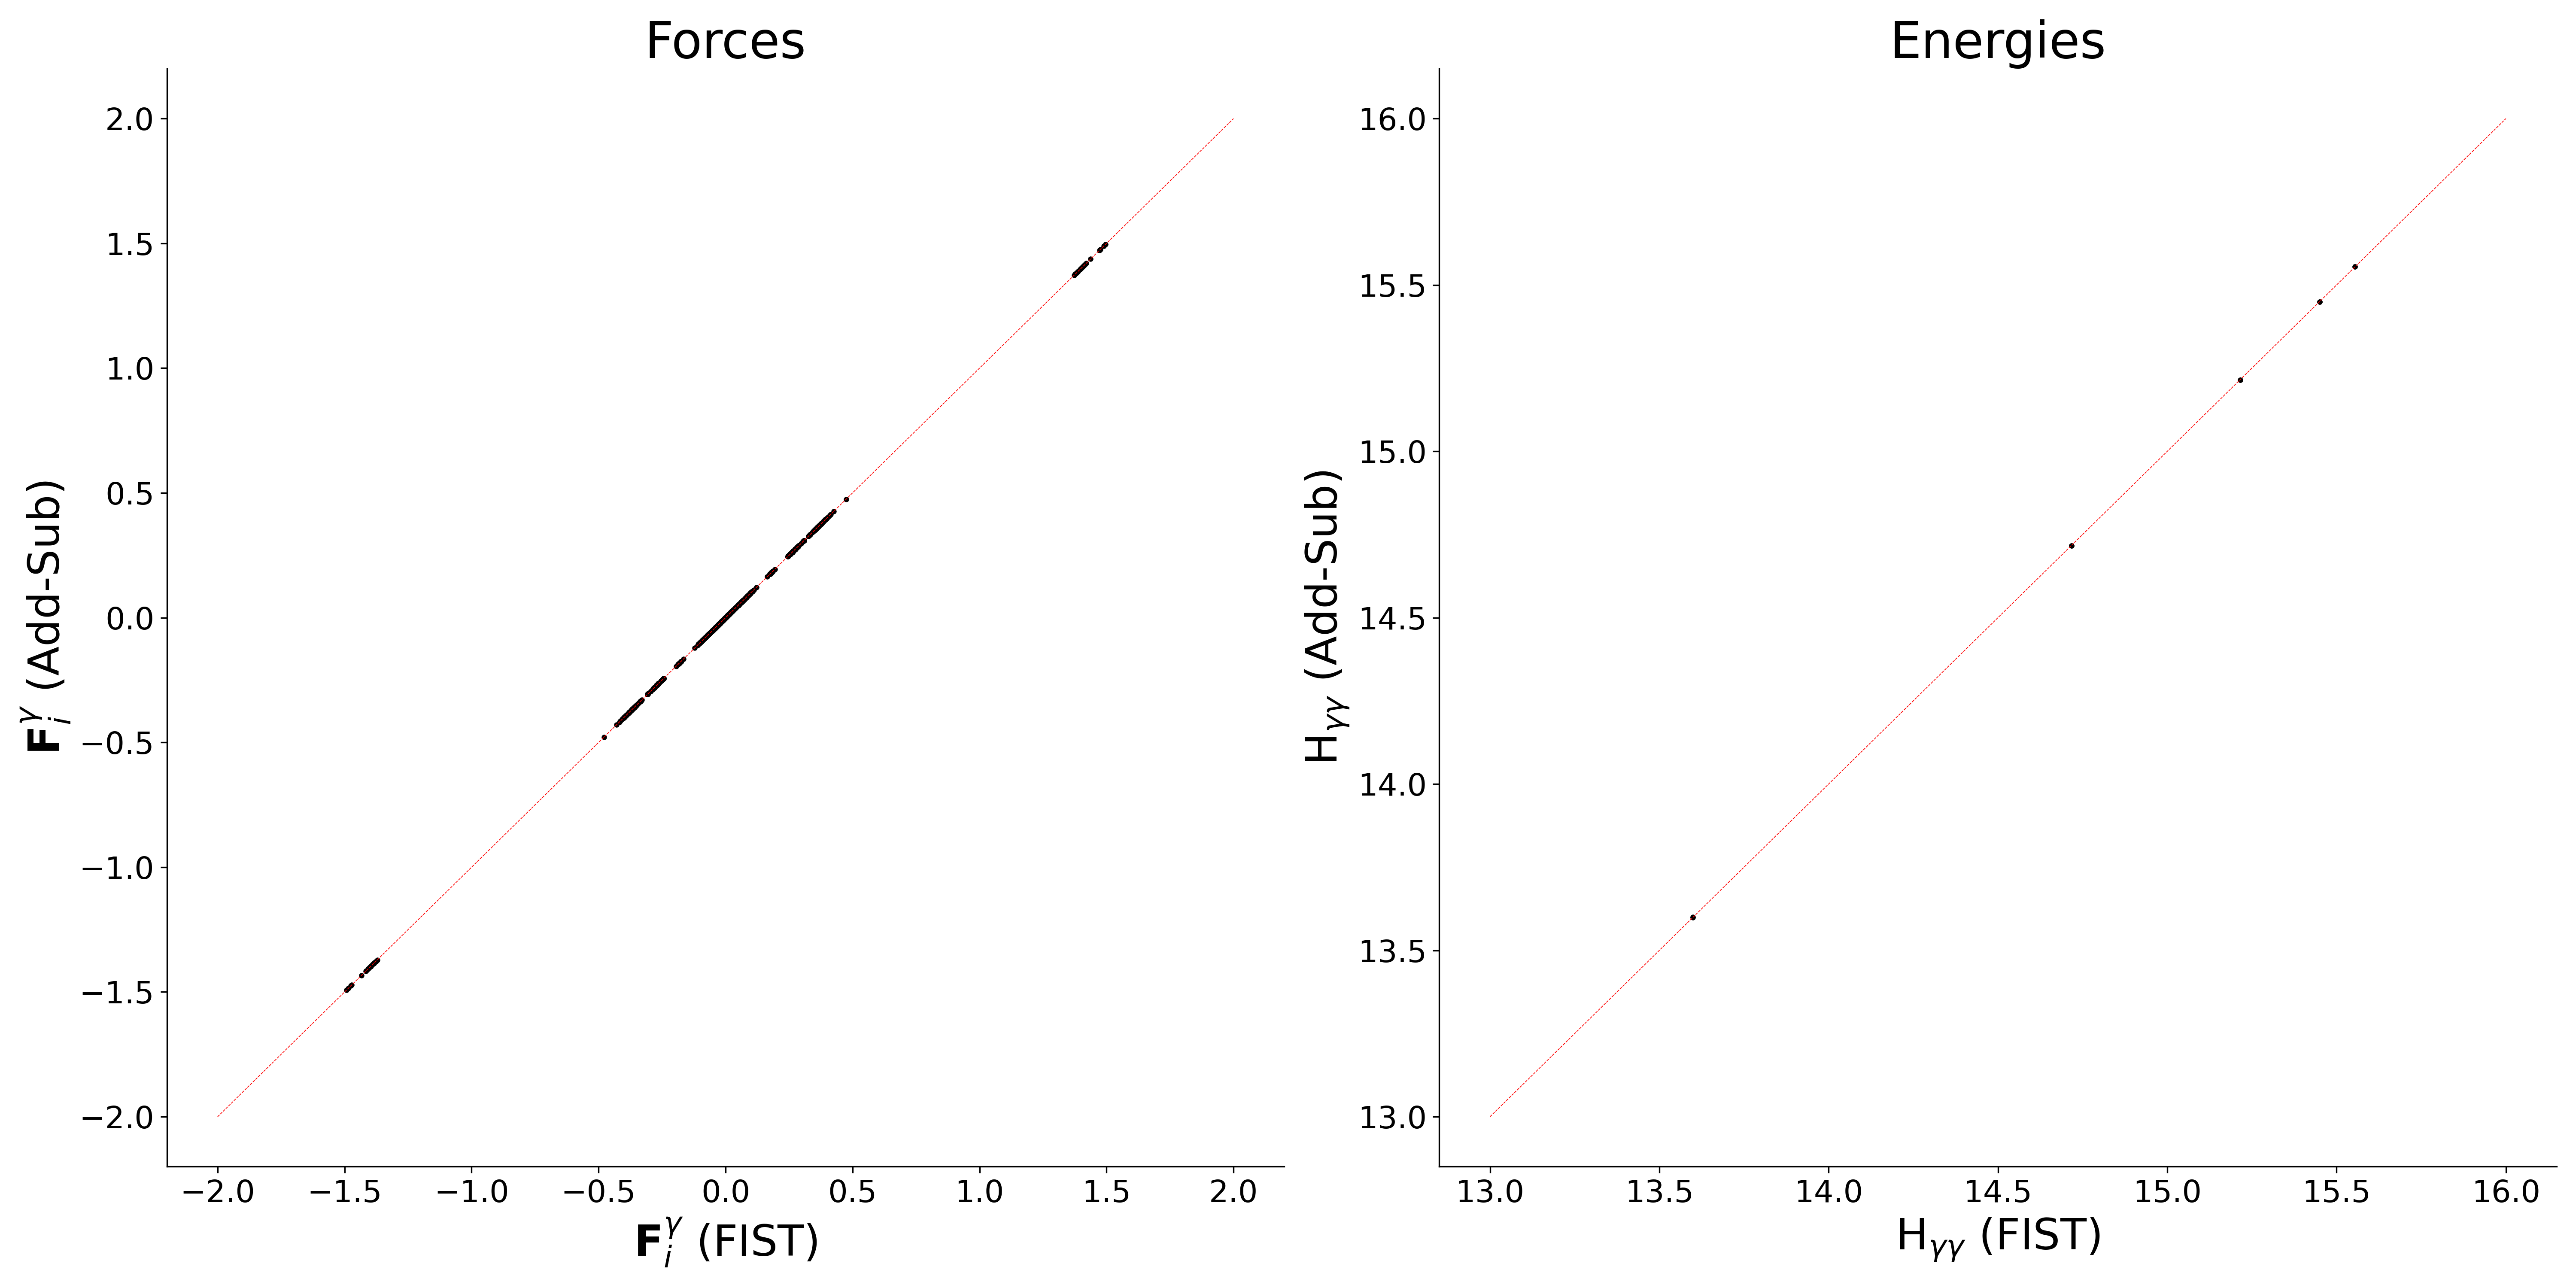
\includegraphics[width=\textwidth]{./img/ES/10_mol_FIST.png}
  \caption{\label{fig:AddSubEwaldTest}A comparison of forces and energies calculated with multiple classical MD simulations (x-axis) and the addition-subtraction method with Ewald electrostatics. The left pane shows the magnitude of the outputted forces and the right the outputted potential energies. Black dots show values from each atom and timestep. The red dashed line shows y=x and serves as a guide for the eye.}
\end{figure}
We see in figure \ref{fig:AddSubEwaldTest} that the values of energy and forces as calculated with CP2K's standard MD package (FIST) and my implementation of the addition-subtraction method are exactly the same. In fact the maximum absolute difference between results was 5$\times 10^{-13}$ i.e. numerical noise. This confirms the implementation of the addition-subtraction scheme. 
\\\\
To further benchmark the addition-subtraction scheme the same input parameters were fed into the code using the recalculation method and the addition-subtraction method. FOB-SH was then ran for 200 timesteps with various system sizes. These ranged from an ethylene dimer to 100 molecule ethylene system. A small 10 molecule pentacene system was also simulated. In order to check for correct output the tool `diff' was used. This checks for differences in files and reports any discrepancies. Using this tool only numerical noise was picked up (errors with a magnitude less than $10^{-12}$). This serves as a further validation of the equations for the addition-subtraction scheme and its implementation within CP2K.  However, as it is currently implemented it doesn't provide a sufficient speed up for realistic applications (hundreds or thousands of molecules), due to high reciprocal space force costs. To optimise the electrostatic calculations further the DSF \cite{DSF} method may be used.
\subsection{DSF}
The damped shifted force method relies on the observation by Wolf et al \cite{Wolf99} that electrostatic interactions are essentially short-ranged (in condensed phase systems). However, in order to converge the real space sum within a cutoff, image charges must be used to ensure charge neutrality within the cutoff sphere. Initially, Wolf et al ensured charge neutrality by placing image charges on the surface off the cutoff sphere. However, this lead to discontinuities in the force at the cutoff radius and poor energy conservation. To fix this Fennel et al (building on the work of Zahn et al) proposed the damped shifted forces technique. The potential and force equations are given below in equations \eqref{eq:DSF_Potential} and \eqref{eq:DSF_Force}. In these equations I have replaced the notation for the magnitude of the displacement vector, $|\mathbf{r}_{ij} + \mathbf{n}|$, with $r_{ij}$ for clarity.
\begin{equation}
  V_{DSF}(r) = q_{i} q_{j} \left[ \frac{erfc(\alpha r_{ij})}{r_{ij}}  - \frac{erfc(\alpha R_{c})}{R_{c}} + \left( \frac{erfc(\alpha R_{c})}{R_{c}^2} + \frac{2 \alpha}{\sqrt{\pi}} \frac{e^{-\alpha^2 R_{c}^2}}{R_{c}} \right) (r_{ij} - R_{c}) \right]
  \label{eq:DSF_Potential}
\end{equation}

\begin{equation}
  \mathbf{F}_{DSF}(r) = q_i q_j \left[ \left( \frac{erfc(\alpha r_{ij})}{r_{ij}^2} + \frac{2 \alpha}{\sqrt{\pi}} \frac{e^{-\alpha^2 r_{ij}^2}}{r_{ij}}\right) - \left(\frac{erfc(\alpha                   R_{c})}{R_{c}^2} + \frac{2 \alpha}{\sqrt{\pi}} \frac{e^{-\alpha^2 R_{c}^2}}{R_{c}} \right) \right] \hat{\mathbf{r}}_{ij}
  \label{eq:DSF_Force}
\end{equation}
In equation \eqref{eq:DSF_Potential} above the first term is the same as in the standard Ewald equation and is equivalent to the original coulomb potential, damped by the complementary error function. The second term is to ensure that the potential goes to zero at the cutoff radius (i.e. $r_{ij} = R_{c}$). The third term, in parentheses, ensures that the derivative of the potential (the force) continuously becomes zero at the cutoff radius. Fortunately, the implementation only involves altering the standard Ewald sum by omitting the reciprocal space, self terms and the bonding correction and amending the real space term. Importantly, this method is fully compatible with the addition-subtraction scheme and can provide a significant speedup to the calculation of the electrostatic interactions. The addition-subtraction scheme equation is the same as for the real space part of the Ewald equations and is given in equation \eqref{eq:RealScheme} where $R^{dir}$ is given by the term in brackets in equation \eqref{eq:DSF_Potential}.
\section{Testing DSF}
\subsection{Classical MD}
\label{sect:ClassicalMDEwald}
In order to validate the DSF implementation various tests were carried out. Firstly, each electrostatic interaction was calculated by hand for a toy carbon monoxide dimer, without periodicity. Charges of +1/-1 were chosen for the oxygen and carbon atoms respectively and each molecule was placed 4 angstroms apart in the y dimension. In this system there are only 3 unique interactions to calculate: C-C, C-O and O-O. The calculated value within the code was compared with the hand-calculated value as well as total energies and forces printed after each step. When the code had passed this test a comparison to Ewald electrostatics was made.
\\
\begin{figure}[ht]
  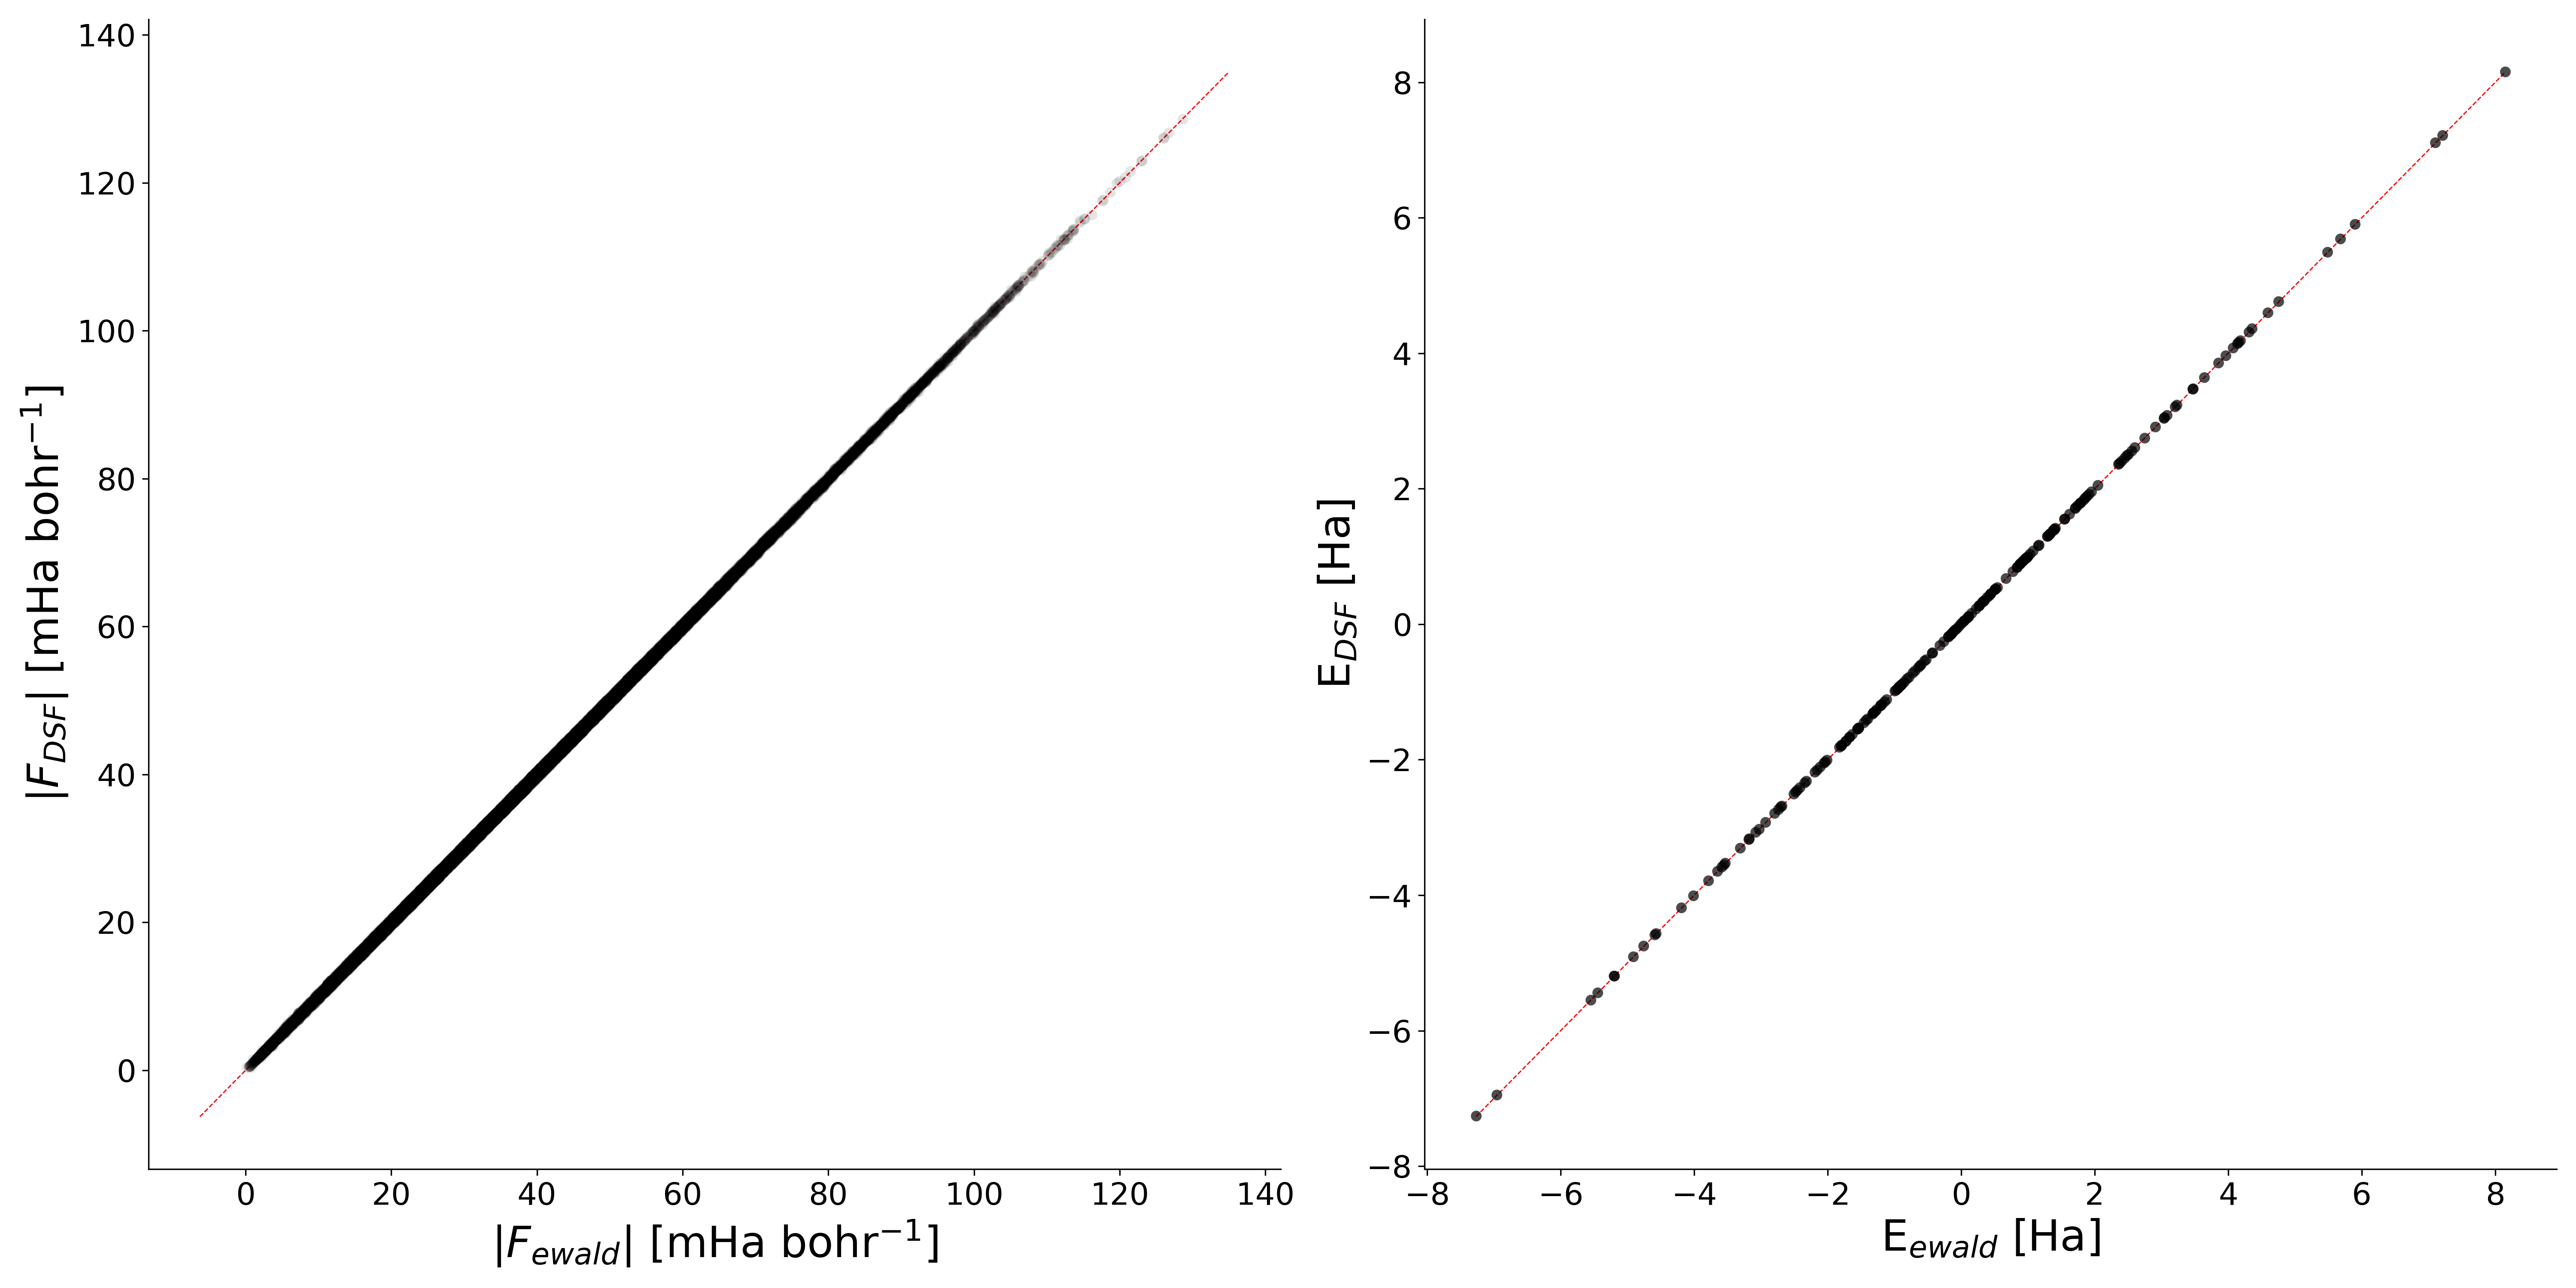
\includegraphics[width=\textwidth]{./img/ES/Ewald_DSF_Classical.png}
  \caption{\label{fig:Classical_DSF_Ewald}Comparison of Ewald and DSF forces and energies. The x-axis shows results from Ewald simulations and the y-axis shows results from DSF simulations. The left pane shows the force magnitude with black dots representing values from all atoms at all timesteps. The right pane shows potential energies from each timestep. The red line shows the line y=x and is a guide for the eye.}
\end{figure}
\\
In order to carry out a comparison to Ewald electrostatics, a small pentacene crystal was constructed, containing 128 molecules. The standard triclinic pentacene unit cell was taken from the Cambridge Structural Database \cite{CSD} and the same forcefield parameters were used as in section \ref{chap:surface_hopping_app}. All molecules were in their neutral state (without an excess charge carrier). A 1ps classical molecular dynamics simulation was then performed with full Ewald electrostatics and positions and velocities were printed every 5fs. 200 separate simulations using DSF electrostatics were then performed using the printed geometries from the Ewald simulations. In these simulations an alpha of 0.0 and cutoff radius of 12$\angstrom$ was used. These were chosen as in Fennel, 06 \cite{DSF} these values gave good results when compared to Ewald electrostatics. It is important to note that in this work the effect of the cutoff radius and the damping coefficient, $\alpha$ have not been investigated. The outputted energies and forces were subsequently compared and the RMSD was found for the difference between the Ewald and DSF simulations. Care was taken to shift both the Ewald and DSF energies by their mean value to correct for a different energy offset in their values. In order to put this RMSD in context, a further simulation was carried out without any electrostatic interactions on the outputted Ewald geomteries. The energies and forces of this simulation were then subtracted from the Ewald energies and forces to isolate just the electrostatic interactions. The root mean squared fluctuations (RMSF) of just the electrostatic energies and forces were then calculated in order to quantify the error that DSF introduces. The root mean squared fluctuations of the Ewald electrostatic energies were calculated to be: 120.0 mHa and the root mean squared deviation in the DSF potential compared to the Ewald potential was calculated to be: 9.49 mHa. The root mean squared fluctuations of the Ewald electrostatic forces were calculated to be: 1.44 mHa bohr$^{-1}$ and the root mean squared deviation of DSF forces compared to Ewald forces were calculated to be: 0.13 mHa bohr$^{-1}$. These results show my implementation of DSF within CP2K to introduce an error of $\sim 8-10$\% within the energies and forces. Further, we see in figure \ref{fig:Classical_DSF_Ewald} the magnitude of each Ewald and DSF force and each energy compared directly. When the coefficient of determination, R$^2$, is calculated for these data sets we get: 1.000 for the energies and forces -very similar values to the ones reported in Fennel, 06.
\\\\
As a final check of the equations the damping coefficient was set to a very large value (10000) and each DSF interaction between pairs of atoms was printed. This was to confirm that, in the limit of an infinite $\alpha$ coefficient, DSF electrostatic contributions to the energies and forces tended to 0. 
\subsection{Surface Hopping}
Although, in surface hopping, the DSF equations are exactly the same the way that they are applied is quite different (as explained in \ref{sect:addSubMethod}). In order to test the DSF implementation in the surface hopping code the same 2 tests were run as in the classical code. The first was to compare each force and site-energy calculated using DSF with the addition-subtraction method to forces and site-energies calculated with N$_{mol}$ different topology files. The second was to compare the surface hopping DSF implementation with the already tested surface-hopping Ewald implementation.
\subsubsection{Multiple Topology Files}
\begin{figure}[ht]
  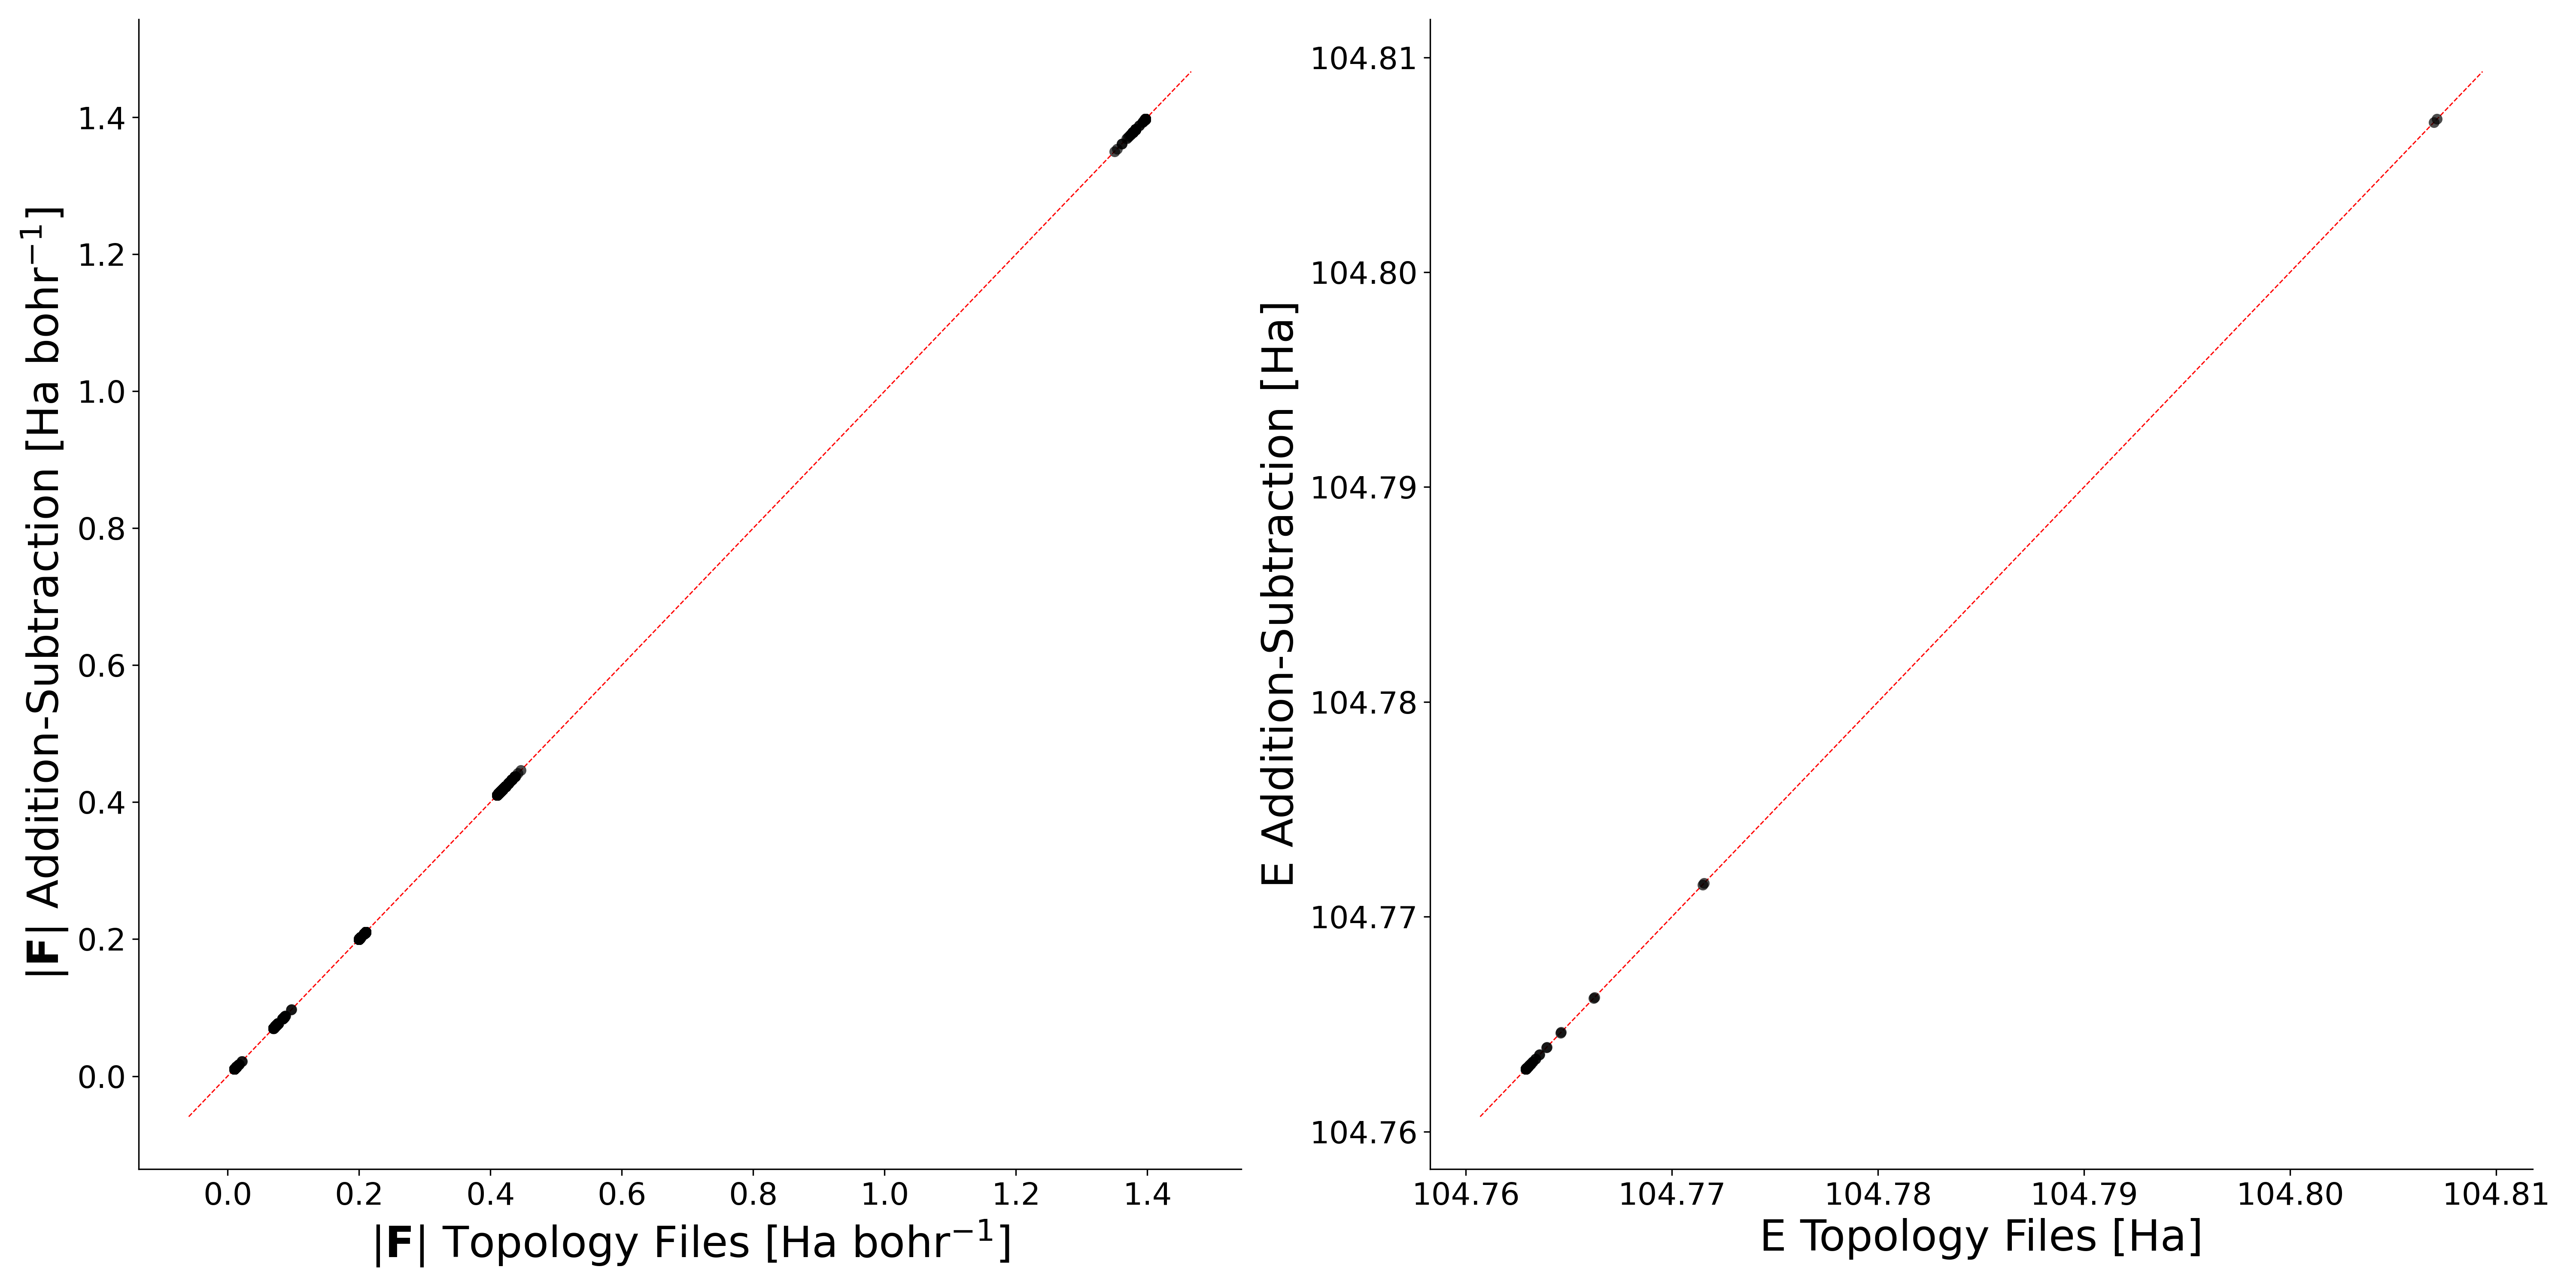
\includegraphics[width=\textwidth]{./img/ES/DSF_SH_test_topologies.png}
  \caption{\label{fig:FSSH_DSF_top}Comparison of Ewald and DSF forces and energies. The x-axis shows results from Ewald simulations and the y-axis shows results from DSF simulations. The left pane shows the force magnitude with black dots representing values from all atoms at all timesteps. The right pane shows potential energies from each timestep. The red line shows the line y=x and serves as a guide for the eye.}
\end{figure}
\noindent As in section \ref{sect:testESimp}, the site-energies and forces for each permutation of the charged molecule were calculated by running N CP2K simulations. In each simulation, the inputted topology had a different molecule in the charged state and all the others in the neutral state. A 100 molecule ethylene system was used and 100 different simulations were ran to get each site-energy and force (using DSF electrostatics). The forces and energies were outputted and used to compare to the forces and energies outputted from the surface hopping simulation using the addition subtraction scheme with DSF electrostatics. The results can be seen in figure \ref{fig:FSSH_DSF_top}. The maximum absolute difference in the outputted values was less than 10$^{-13}$ confirming the implementation of DSF with the addition-subtraction scheme in surface hopping.
\subsubsection{Comparison to Ewald}
\begin{figure}[htp]
  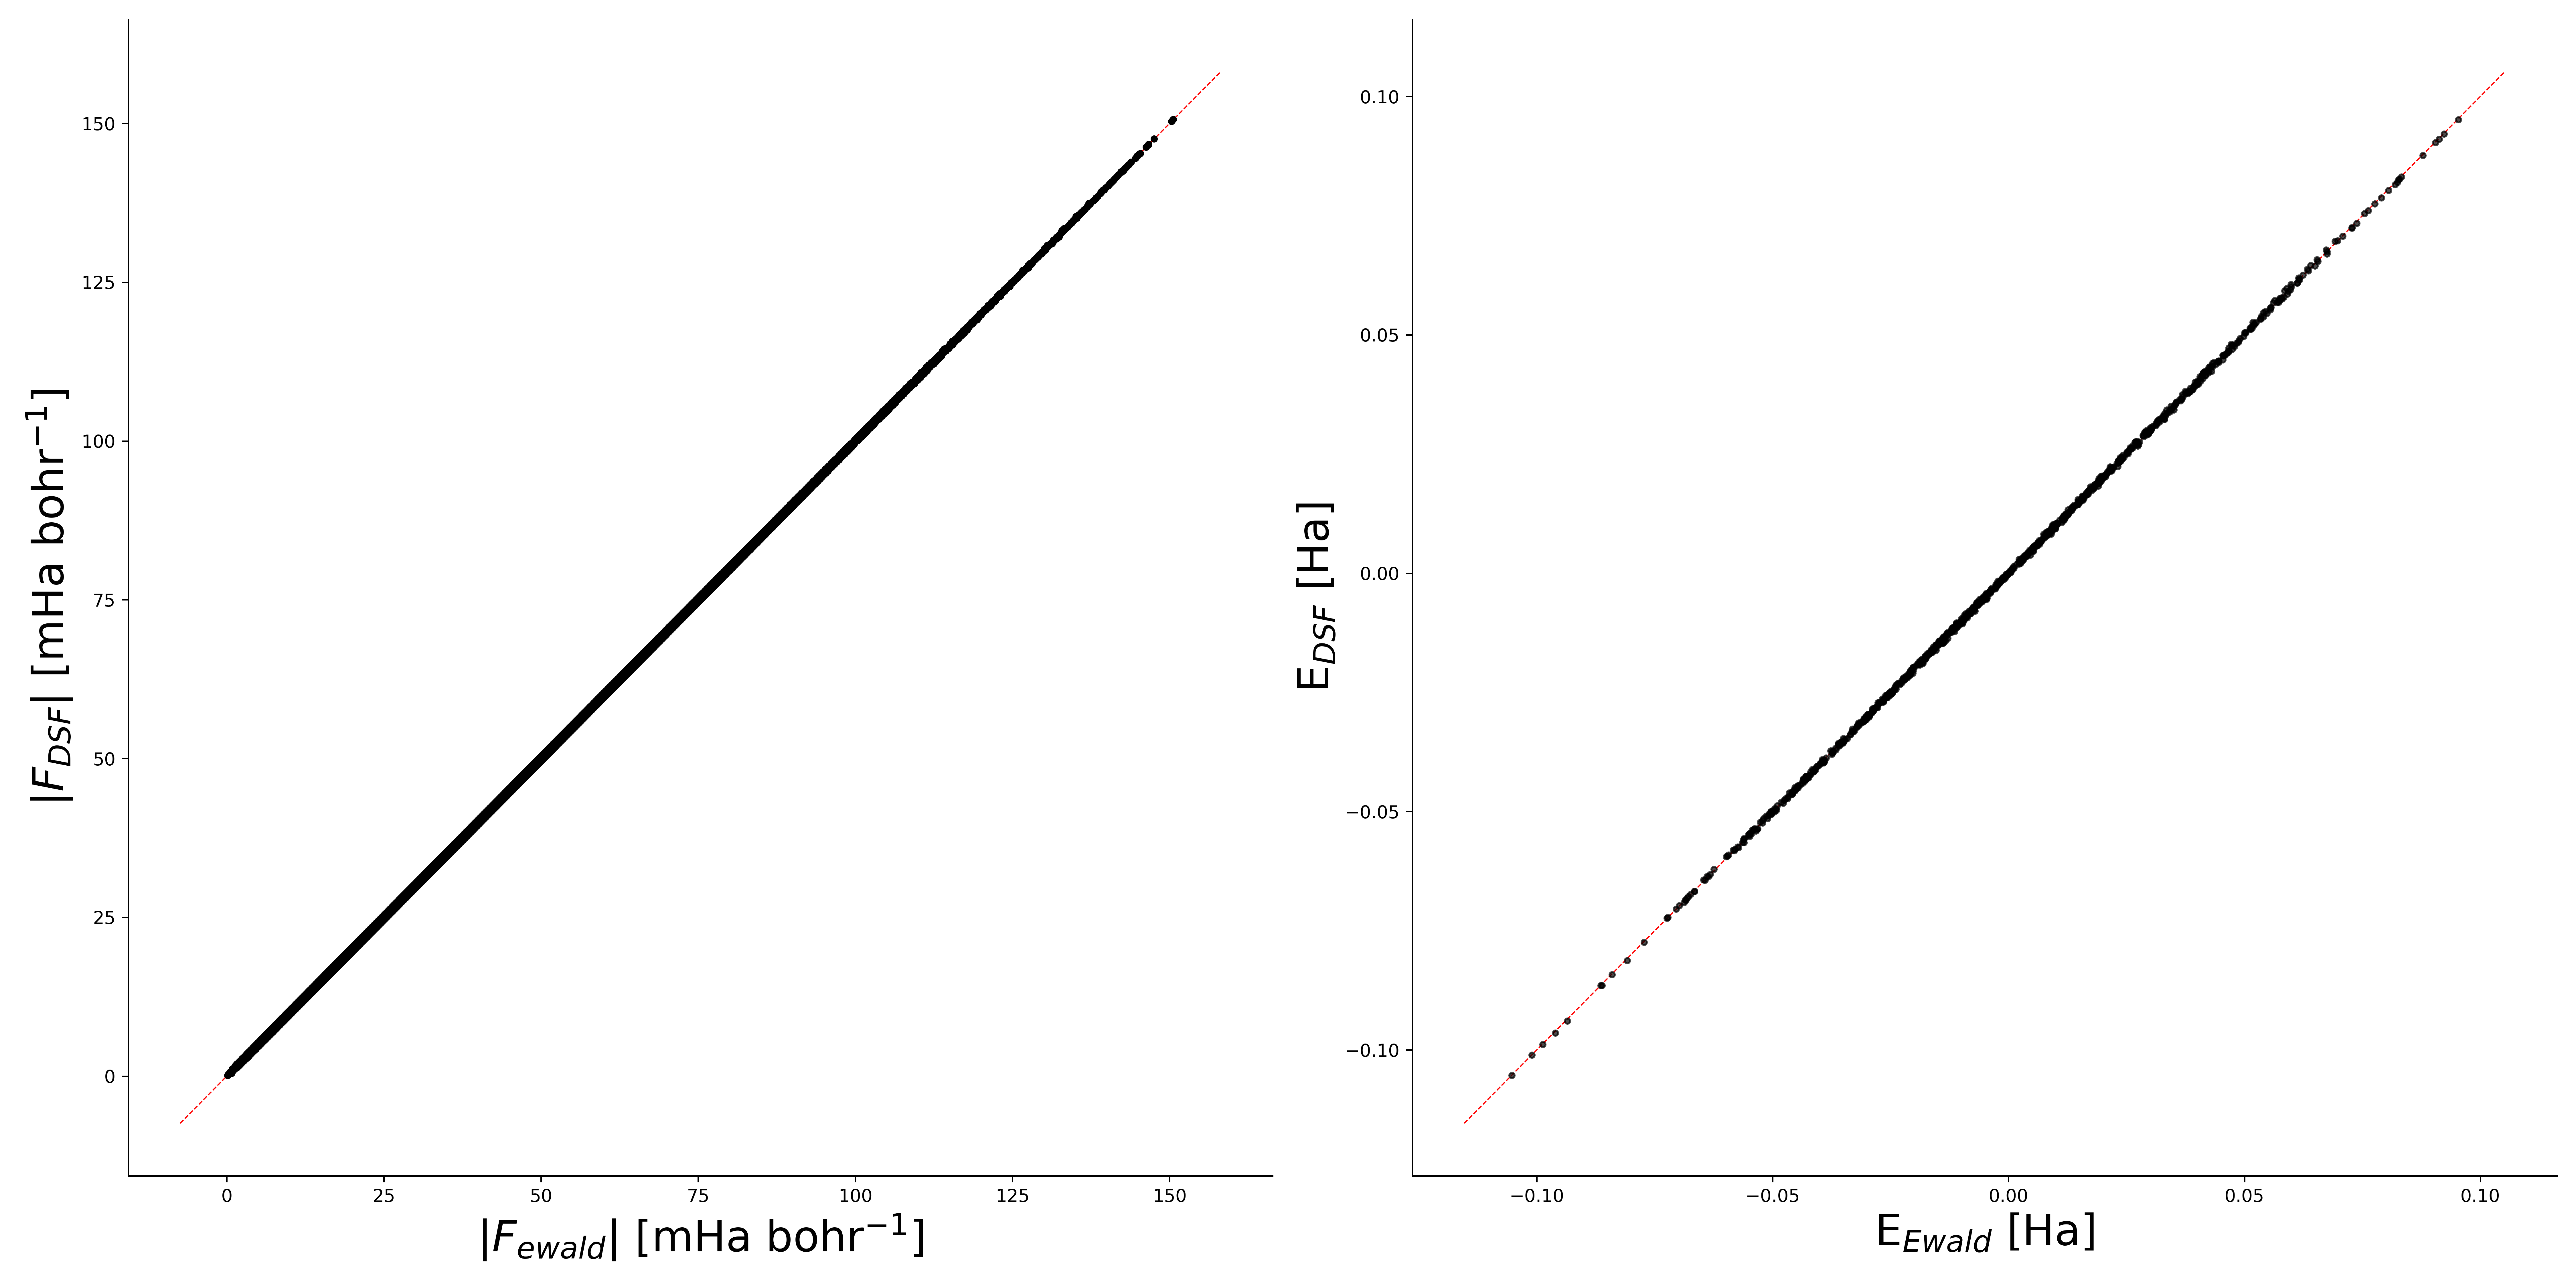
\includegraphics[width=\textwidth]{./img/ES/DSF_vs_Ewald_FSSH.png}
  \caption{\label{fig:DSF_vs_EwaldSH}A comparison of energies and forces as calculated by full Ewald and DSF electrostatics.}
\end{figure}
The comparison to Ewald electrostatics was carried out as in \ref{sect:ClassicalMDEwald}. That is, a surface hopping simulation was carried out with a small pentacene crystal and Ewald electrostatics. Positions and velocities were printed out periodically and DSF electrostatics was then ran using each of the position and velocity files as initial geometries. A cutoff radius of 15$\angstrom$ and damping coefficient of 0.0$bohr^{-1}$ was used. Forces and energies were then compared and the root mean squared deviation between Ewald and DSF was calculated. The system was a 54 molecule pentacene crystal that had been equilibrated with classical MD using SPME as the electrostatic calculator, until the temperature and total energy had converged. The results are shown in figure \ref{fig:DSF_vs_EwaldSH}. 
\\\\
The results, reflect very well the findings from figure \ref{fig:Classical_DSF_Ewald}. This is to be expected as the same equations are being used. We see in both the forces and the energies that there is very little deviation of values with respect to full Ewald simulations at every timestep. In fact, the $R^2$ value is 1.000 for both datasets. The RMSD \ldots This validates my implementation of DSF within surface hopping against my implementation of Ewald electrostatics. Further the Ewald implementation has been validated against classical MD and has been shown to reproduce the energies and forces exactly. Satisfied that the DSF implementation is working, in the following section, I will briefly show the speed up achieved by using DSF instead of Ewald electrostatics before final concluding remarks.

\section{Timing DSF}
\begin{figure}[htp]
  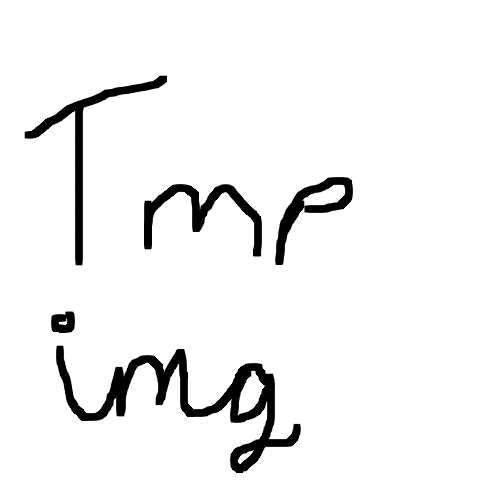
\includegraphics[width=\textwidth]{./img/tmp.png}
  \caption{\label{fig:DSF_Timings}Timing data on the DSF implementation compared to Ewald electrostatics}
\end{figure}
The DSF technique has been shown to give values for electrostatic energies and forces that very closely resemble Ewald electrostatics. However, if it does not provide a speedup to the code it has no use. In order to quantify the difference in time taken to calculate electrostatic interactions, I have ran a variety of simulations using Ewald electrostatics and DSF electrostatics in surface hopping and shown the results in figure \ref{fig:DSF_Timings}. In this figure we can clearly see\ldots


%\section{Miscellaneous Optimisations}
%To help prepare the code for the study of larger systems, other group members and I implemented various other 

\section{Conclusions}
In this chapter I have presented an extension to the surface hopping code, namely the implementation of electrostatic interactions. I have tested and timed my implementation of the standard Ewald summation technique and the damped shifted forces (DSF) method. I have discussed the limitations in the standard Ewald technique, i.e. far too costly for large systems and discussed how these can be mitigated with the DSF method. Due to the way the Hamiltonian is constructed in FOB-SH, each diagonal element (site-energy) is calculated by calculating all forces and energies. There are $N_{mol}$ site-energies leading to a scaling in CPU time of $O(N_{mol} N_{atom}^2)$. However, the use of an addition-subtraction scheme has been shown to successfully reduce this by an order of magnitude ($N_{mol}$), allowing the simulation of large systems requiring the proper account of electrostatic interactions (such as polar systems or highly disordered ones). However, this addition-subtraction scheme cannot be applied to the reciprocal space forces in the Ewald summation. For this reason, DSF has been implemented to provide a reasonable estimate of full Ewald forces and energies. In the systems tested in this chapter the error produced by DSF was around 8-10\% compared with Ewald electrostatics. Although with appropriate tuning of input parameters this may be reduced even further. An investigation of the parameters has not been carried out in this work due to time constraints, though should be a relatively straightforward task. The timings \ldots

\chapter{General conclusions}
\label{chap:conclusion}

\addcontentsline{toc}{chapter}{Appendices}



% The \appendix command resets the chapter counter, and changes the chapter numbering scheme to capital letters.
%\chapter{Appendices}
\appendix
\chapter{Tully Model Paramters}
\label{ap:tully_params}

\section{Model 1 -Single Avoided Crossing}
  \begin{minipage}{0.5\textwidth}
      \textbf{Hamiltonian Paramters:}
      \begin{flalign*}
        H_{11}(\mathbf{R}) \ &= \ A \ \tanh(B\mathbf{R}) &\\
        H_{12}(\mathbf{R}) \ &= \ C e^{-D\mathbf{R}^2} \\
        H_{21}(\mathbf{R}) \ &= \ H_{12}(\mathbf{R}) \\
        H_{22}(\mathbf{R}) \ &= \ -H_{11}(\mathbf{R})
      \end{flalign*}
      Where A = 0.03, B = 0.4, C = 0.005 and D = 0.3
  \end{minipage}
  \hspace{0.5cm}
  \vrule
  \hspace{0.5cm}
  \begin{minipage}{0.6\textwidth}
      \begin{tabular}{l|l|c}
        \textbf{Quantity} & \textbf{Value} & \textbf{Unit} \\
        \hline
        Initial Position & -20 & a.u. \\
        Initial Velocities & 15.0, 25.0 & a.u. \\
        Initial Adiab Pop & ground state & - \\
        Simulation Time & 6000, 4000 & a.u. \\
        $\sigma_{\nu}^{(I)}$ & 0.5 & a.u. \\
        M ($\sigma$ constant) & 40 & - \\
        $\Delta t_{\text{nuclear}}$ & 0.1 & fs \\
        $\Delta t_{\text{electonic}}$ & 0.01 & fs \\
        $\frac{\delta \mathbf{R}_{lk, \nu}^{(I)}}{\delta t}$ threshold & 0.15 & a.u. \\
        N$_{rep}$ & 200 & - \\
      \end{tabular}
  \end{minipage}

\section{Model 2 -Dual Avoided Crossing}
\begin{minipage}{0.48\textwidth}
    \textbf{Hamiltonian Paramters:}
    \begin{flalign*}
      H_{11}(\mathbf{R}) \ &= \ 0 &\\
      H_{12}(\mathbf{R}) \ &= \ C e^{-D \mathbf{R}^2} \\
      H_{21}(\mathbf{R}) \ &= \ H_{12}(\mathbf{R}) \\
      H_{22}(\mathbf{R}) \ &= \ -A e^{-B\mathbf{R}^2} + E
    \end{flalign*}
    Where A = 0.1, B = 0.28, C = 0.015, D = 0.06 and E = 0.05
  \end{minipage}
  \hspace{0.5cm}
  \vrule
  \hspace{0.5cm}
  \begin{minipage}{0.6\textwidth}
      \begin{tabular}{l|l|c}
        \textbf{Quantity} & \textbf{Value} & \textbf{Unit} \\
        \hline
        Initial Position & -8 & a.u. \\
        Initial Velocities & 16.0, 30.0 & a.u. \\
        Initial Adiab Pop & ground state & - \\
        Simulation Time & 2500, 1500 & a.u. \\
        $\sigma_{\nu}^{(I)}$ & 0.5 & a.u. \\
        M ($\sigma$ constant) & 40 & - \\
        $\Delta t_{\text{nuclear}}$ & 0.1 & fs \\
        $\Delta t_{\text{electonic}}$ & 0.01 & fs \\
        $\frac{\delta \mathbf{R}_{lk, \nu}^{(I)}}{\delta t}$ threshold & 0.15 & a.u. \\
        N$_{rep}$ & 200 & - \\
      \end{tabular}
  \end{minipage}

\section{Model 3 -Extended Coupling}
\begin{minipage}{0.5\textwidth}
    \textbf{Hamiltonian Paramters:}
    \begin{flalign*}
      H_{11}(\mathbf{R}) \ &= \ A  &\\
      H_{12}(\mathbf{R}) \ &= \ \left \lbrace
      \begin{array}{l}
        B e^{C\mathbf{R}}, \qquad \qquad R \leq 0 \\
          B(2 - e^{-C\mathbf{R}}), \quad R > 0\\
      \end{array} \right . \\
      H_{21}(\mathbf{R}) \ &= \ H_{12}(\mathbf{R}) \\
      H_{22}(\mathbf{R}) \ &= \ -H_{11}(\mathbf{R})
    \end{flalign*}
    Where A = 6$\times$ 10$^{-4}$, B = 0.1 and C = 0.9
  \end{minipage}
  \hspace{0.2cm}
  \vrule
  \hspace{0.6cm}
  \begin{minipage}{0.6\textwidth}
      \begin{tabular}{l|l|c}
        \textbf{Quantity} & \textbf{Value} & \textbf{Unit} \\
        \hline
        Initial Position & -15 & a.u. \\
        Initial Velocities & 10, 30 & a.u. \\
        Initial Adiab Pop & ground state & - \\
        Simulation Time & 5000, 1500 & a.u. \\
        $\sigma_{\nu}^{(I)}$ & 0.5 & a.u. \\
        M ($\sigma$ constant) & 40 & - \\
        $\Delta t_{\text{nuclear}}$ & 0.1 & fs \\
        $\Delta t_{\text{electonic}}$ & 0.01 & fs \\
        $\frac{\delta \mathbf{R}_{lk, \nu}^{(I)}}{\delta t}$ threshold & 0.15 & a.u. \\
        N$_{rep}$ & 200 & - \\
      \end{tabular}
  \end{minipage}


\section{Model 4 -Dual Arch}
\hspace*{-1.5cm}
\begin{minipage}{0.49\textwidth}
    \textbf{Hamiltonian Paramters:}
    \begin{flalign*}
      H_{11}(\mathbf{R}) \ &= \ A  &\\
      H_{12}(\mathbf{R}) \ &= \ \left \lbrace
      \begin{array}{l}
        B \left[ -e^{C(\mathbf{R} - D)} + e^{C(\mathbf{R} + D)} \right] \ \qquad \qquad \ R \leq -D \\
        B \left[ e^{-C(\mathbf{R} - D)} - e^{-C(\mathbf{R} + D)} \right] \ \ \ \ \ \qquad \quad R \geq D \\
        B \left[ 2 - e^{C(\mathbf{R} - D)} - e^{-C(\mathbf{R} + D)} \right] \ \ -D < R < D \\
      \end{array} \right . \\
      H_{21}(\mathbf{R}) \ &= \ H_{12}(\mathbf{R}) \\
      H_{22}(\mathbf{R}) \ &= \ -H_{11}(\mathbf{R})
    \end{flalign*}
    Where A = 6$\times$ 10$^{-4}$, B = 0.1, C = 0.9 and D = 4
  \end{minipage}
  \hspace*{-0.2cm}
  \vrule
  \hspace{0.2cm}
  \begin{minipage}{0.6\textwidth}
      \begin{tabular}{l|l|c}
        \textbf{Quantity} & \textbf{Value} & \textbf{Unit} \\
        \hline
        Initial Position & -20 & a.u. \\
        Initial Velocities & 10, 40 & a.u. \\
        Initial Adiab Pop & ground state & - \\
        Simulation Time & 6000, 2000 & a.u. \\

        $\sigma_{\nu}^{(I)}$ & 0.5 & a.u. \\
        M ($\sigma$ constant) & 40 & - \\
        $\Delta t_{\text{nuclear}}$ & 0.1 & fs \\
        $\Delta t_{\text{electonic}}$ & 0.01 & fs \\
        $\frac{\delta \mathbf{R}_{lk, \nu}^{(I)}}{\delta t}$ threshold & 0.15 & a.u. \\
        N$_{rep}$ & 200 & - \\
      \end{tabular}
  \end{minipage}
















\chapter{Wigner Distribution Derivation}
\label{ap:Wigner}
The nuclear wavepacket (at time 0) is given by:
\begin{equation}
  \chi(R) = \frac{1}{(\pi \mu^2)^{\frac{1}{4}}} e^{-\frac{(R - R_0)^2}{2 \mu^2} + \im k_0 (R - R_0) }
  \label{eq_ap:initial_nucl_wp}
\end{equation}
The Wigner quassiprobability function for momentum and position (p, R) is given by:
\begin{equation}
  W(p, R) = \frac{1}{\pi \hbar} \int_{-\infty}^{\infty} \chi^{*}(R + y) \chi(R -y) e^{\frac{2 \im p y}{\hbar}} dy
  \label{eq_ap:Wig_def}
\end{equation}
However, both Ehrenfest and CTMQC require atomic positions as input so we must extract the position and velocity probability densities from this. We get these from the marginal integrals of the Wigner distribution i.e.
\begin{equation}
  \vert f(R)\vert^2 = \int^{\infty}_{-\infty} W(R, p) dp
\end{equation}
\begin{equation}
  \vert f(p)\vert^2 = \int^{\infty}_{-\infty} W(R, p) dR
\end{equation}
In order to calculate these marignal integrals we must first crunch through the maths of equation \eqref{eq_ap:Wig_def}. Substituting eq \eqref{eq_ap:initial_nucl_wp} into \eqref{eq_ap:Wig_def}:
\begin{equation}
  W(p, R) = \frac{1}{\pi \hbar} \int_{-\infty}^{\infty} \frac{1}{\mu \sqrt{\pi}} e^{- \frac{(R + y - R_0)^2}{2 \mu^2} - 2\im k_0y - \frac{(R - y - R_0)^2}{2 \mu^2} } e^{\frac{2 \im p y}{\hbar}} dy
  \label{eq_ap:step1}
\end{equation}
Simplifying the 2 quadratic equations (equation \eqref{eq_ap:step1}) we get:
\begin{equation}
  W(p, R) = \frac{1}{\pi \hbar} \int_{-\infty}^{\infty} \frac{1}{\mu \sqrt{\pi}} e^{-\mu^{-2} \left(y^2 - 2\im k_0y \mu^2 + (R - R_0)^2 \right) } e^{\frac{2 \im p y}{\hbar}} dy
  \label{eq_ap:step2}
\end{equation}
We can now take the expressions not dependant on y outside of the integral and combine the exponents.
\begin{equation}
  W(p, R) = \frac{1}{\pi \sqrt{\pi} \mu \hbar} e^{-\frac{(R - R_0)^2}{\mu^2}} \int_{-\infty}^{\infty} e^{-\frac{y^2 + 2 \im y\mu^{2}\left( \frac{p}{\hbar} - k_0\right)}{\mu^{2}}  } dy
  \label{eq_ap:step3}
\end{equation}
Integrating we get:
\begin{equation}
  \int e^{-\frac{y^2 + 2 \im y\mu^{2}\left( \frac{p}{\hbar} - k_0\right)}{\mu^{2}}  } dy = \frac{\sqrt{\pi} \mu}{2} e^{-\frac{\mu^2}{\hbar^2} (p - \ \hbar k_0)^2} erf\left[\frac{y}{\mu} + \im \left(\frac{p \mu}{\hbar} - \mu k_0 \right)\right]
   \label{eq_ap:step4}
\end{equation}
Applying limits we get:
\begin{equation}
  \int_{-\infty}^{\infty} e^{-\frac{y^2 + 2 \im y\mu^{2}\left( \frac{p}{\hbar} - k_0\right)}{\mu^{2}}  } dy = \sqrt{\pi} \mu e^{-\frac{\mu^2}{\hbar^2} \left(p - \ \hbar k_0 \right)^2}
  \label{eq_ap:step5}
\end{equation}
Substituting this back into the Wigner distribution (equation \eqref{eq_ap:Wig_def}) we finally get:
\begin{equation}
  W(p, R) = \frac{1}{\pi \hbar} e^{-\frac{(R - R_0)^2}{\mu^2}} e^{-\frac{\left(p - \ \hbar k_0 \right)^2}{\hbar^2/\mu^2}}
  \label{eq_ap:step6}
\end{equation}
Taking the maringal integrals we get the position and velocity probability distributions:
\begin{equation}
  \vert f(R)\vert^2 = \frac{2}{\mu \sqrt{\pi}} e^{- \frac{(R - R_0)^2}{\mu^2}}
\end{equation}
\begin{equation}
  \vert f(p)\vert^2 = \frac{2}{\frac{\hbar}{\mu} \sqrt{\pi}} e^{- \frac{\mu^2}{\hbar^2}(p - \ \hbar k_0)^2}
\end{equation}
The above distributions are randomly sampled to get initial atomic velocities and positions for each simulation.

\chapter{$\mathbf{R}_{lk, \nu}$ Alternatives}
\label{ap:RlkAlternatives}
\section{$\mathbf{R}_{lk, \nu}$ Extrapolation}
\label{ap:RlkExtrap}

\section{Alternative Quantum Momentum Intercept}
\label{ap:AltIntercept}
In Agostini, 16 \cite{agostini_quantum-classical_2016} another quantum momentum intercept term is discussed. This term is not used because, as previously discussed in section \ref{sect:CTMQC_Approx}, it leads to unphysical transfer of population between adiabatic states when the nonadiabatic coupling elements are 0. However, it can be used in these Tully Models as an effective fix to the discontinuities caused by the $\mathbf{R}_{lk, \nu}$ term.
\\\\
The other quantum momentum intercept, $\mathbf{R}_{0, \nu}^{(I)}$, comes directly from the construction of the nuclear density using a linear combination of a product of gaussians (see equation \eqref{eq:NuclDens} in the introduction). It is defined as in equation \eqref{eq:RI0} below:
\begin{equation}
    \mathbf{R}_{0, \nu}^{(I)} = \sum_{J}^{N_{tr}} \left[ \frac{\hbar          \prod_{\nu'}                                                                  g_{\sigma_{\nu'}^{(J)}(t)}\left(\mathbf{R}_{\nu'}^{(I)}(t) -                  \mathbf{R}_{\nu'}^{(J)}(t)\right)}   {2                                       \sigma_{\nu}^{(J)}(t)^2\sum_{K}^{N_{tr}}\prod_{\nu'}                                                                                                        g_{\sigma_{\nu'}^{(K)}(t)}\left(\mathbf{R}_{\nu'}^{(I)}(t) -                  \mathbf{R}_{\nu'}^{K)}(t)\right)} \mathbf{R}_{\nu}^{(I)} \right]
    \label{eq:RI0}
\end{equation}

However, as switching to this intercept directly may cause discontinuities in itself a smoothing parameter is applied to ease the switch. This is given in equation \eqref{eq:effR} below:
\begin{equation}
	\left[ 1 - A(t) \right] R_{good}(t) + A(t)R_{bad}(t) = R_{effective}(t)
	\label{eq:effR}
\end{equation}

$R_{good}$ refers to the intercept that should be switched to (e.g. for the detection of a spike in the $R_{lk, \nu}^{(I)}$ we switch to the intercept in in equation \eqref{eq:RI0}). $R_{lk, \nu}^{(I)}$ refers to the intercept that is being switched from (e.g. when it is detected that the divergence of $R_{lk, \nu}^{(I)}$ has finished then we switch from the alternative intercept back to $R_{lk, \nu}^{(I)}$). $A(t)$ is a smoothing parameter and is given in equation \eqref{eq:tanhSmoothParam} below:

\begin{equation}
	A(t) = \frac{D_{\nu}^{(I)}}{2} \left[ tanh\left( t - \frac{t_{final} + t_{init}}{0.6 N dt} \right) + 1 \right]
	\label{eq:tanhSmoothParam}
\end{equation}

Where $D_{\nu}^{(I)}$ is the distance between the 2 intercepts (e.g. $D_{\nu}^{(I)} = R_{lk, \nu}^{(I)} - R_{0, \nu}^{(I)}$), $N$ is the number of steps to take before settling solely on one intercept, $t_{init}$ is the time of detection of the divergence, $t_{final}$ is the time at which the code settles on 1 intercept and dt is the timestep taken.
\\
A cartoon of this process is given in figure \ref{fig:tanh_explan}
\begin{figure}[ht]
	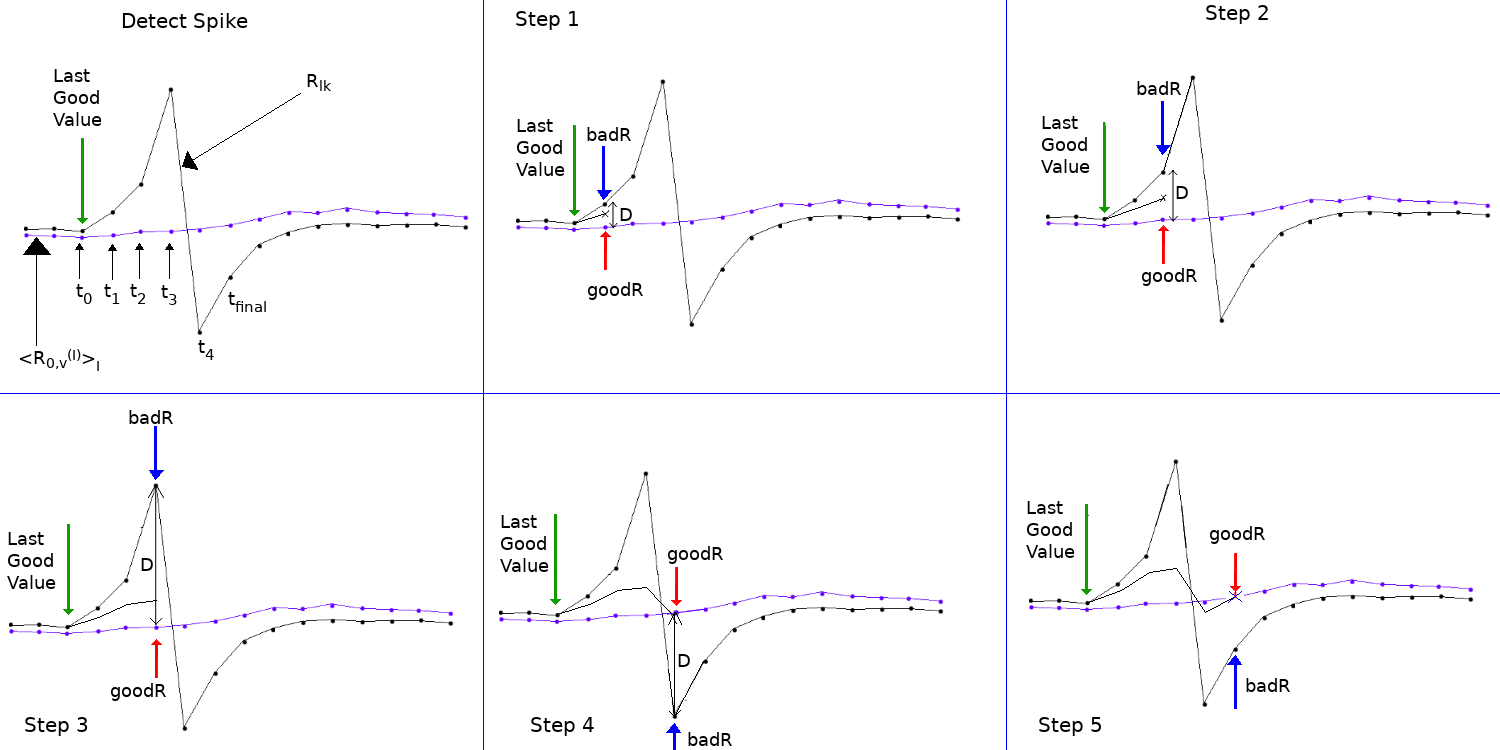
\includegraphics[width=\textwidth]{./img/CTMQC/tanh_explanation.png}
	\caption{\label{fig:tanh_explan}A crude demonstration of the principle behind the smoothing procedure in switching between intercepts. The black line shows an intercept begin to diverge and the alternative intercept is shown in purple. As the step is incremented the amount of the alternative intercept that makes up the effective intercept is increased until only 1 intercept is used.}
\end{figure}


\chapter{Rabi Oscillation \label{ap:Rabi}}
The time dependant Schr\"odinger equation is given below:
\begin{equation}
	i \hbar \frac{\delta}{\delta t} \Phi(\mathbf{R}(t), t) = \hat{H}(\mathbf{R}(t), t) \Phi(\mathbf{R}(t), t)
\end{equation}
If we hold the nuclear coordinates in place (e.g. remove time-dependence from nuclear coordinates) we get an ordinary differential equation as shown below:
\begin{equation}
	i \hbar \frac{d}{d t} \Phi(\mathbf{R}, t) = \hat{H}(\mathbf{R}, t) \Phi(\mathbf{R}, t)
	\label{eq:RABI}
\end{equation}
This has the following general solution. This can be solved with a Taylor series expansion.
\[\Phi(\mathbf{R}, t) = e^{i \hbar \hat{H}t} \Phi(\mathbf{R}, 0)\]
Figure 
\begin{figure}[ht]
  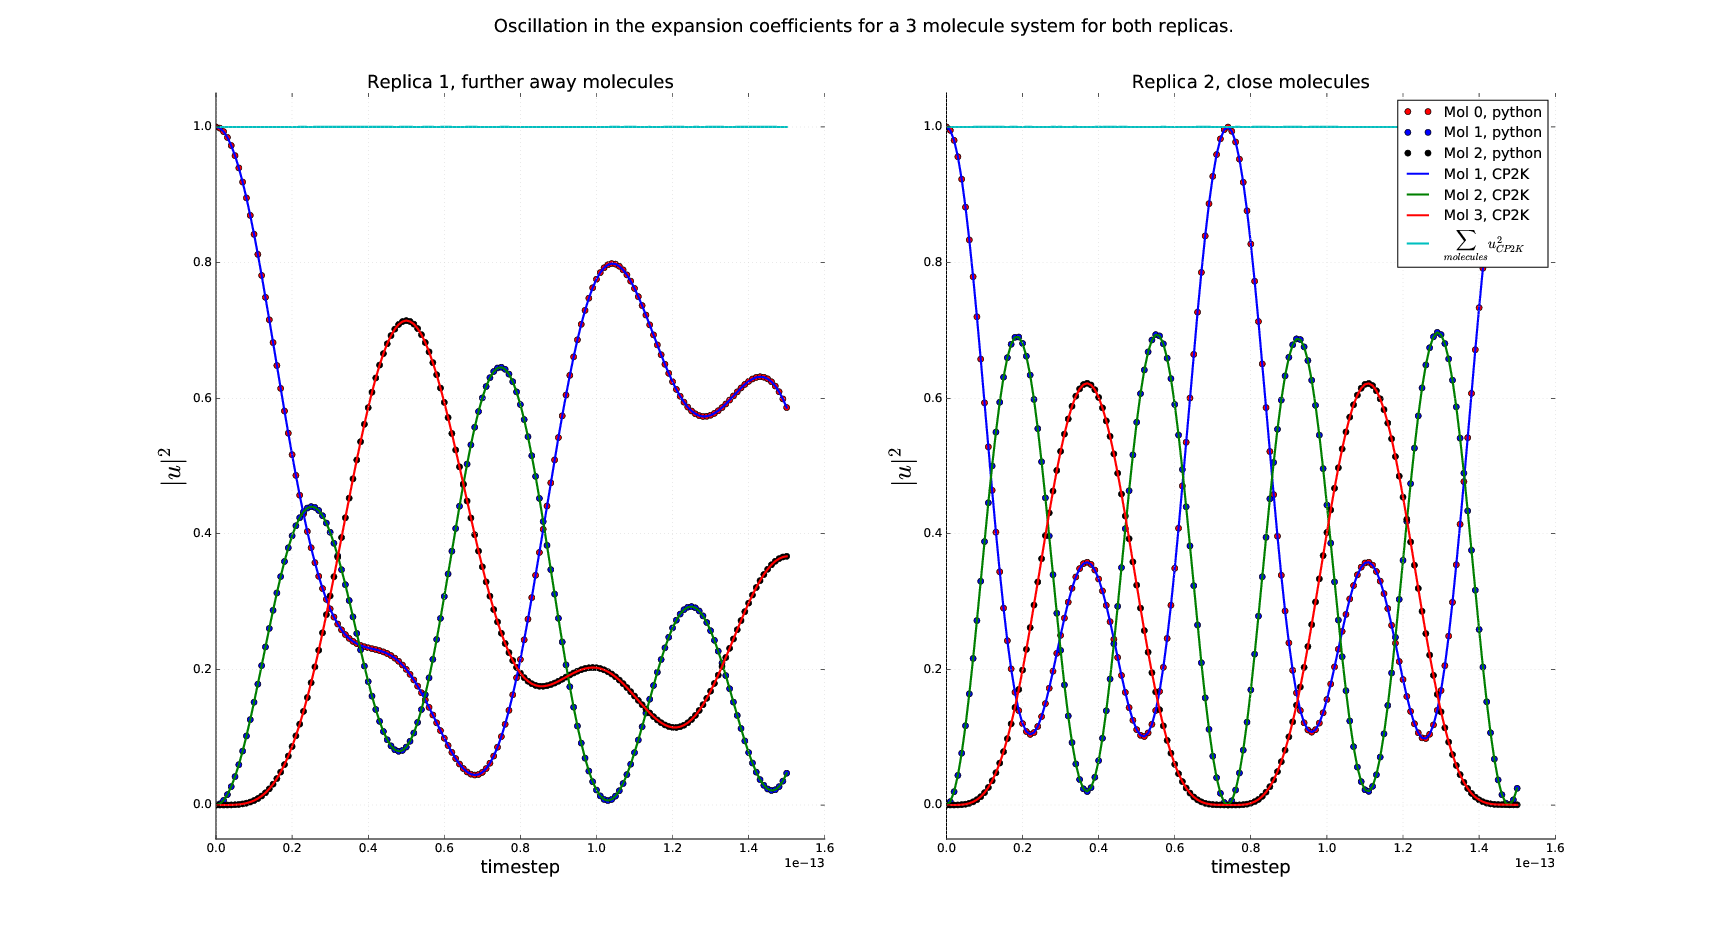
\includegraphics[width=\textwidth]{./img/CTMQC/3_mols_with_python_sol_2_rep.png}
  \caption{\label{fig:Rabi}Rabi oscillation occurring within a Ethylene trimer system. Dotted lines were calculated using equation \eqref{eq:RABI}, solid lines were calculated using the RK4 propagator within the CTMQC section of the CP2K code. The norm is shown on the top as a cyan line and the x axis shows the timestep in seconds.}
\end{figure}









\chapter{Norm Conservation in CTMQC and Ehrenfest}
\label{ap:norm_cons}
A statement of the conservation of the norm, for a single trajectory, is given below in equation \eqref{eq:normConsState}
\begin{equation}
	\frac{d}{dt} \sum_{l} \left\vert C_{l}(t) \right\vert^2 = \sum_{l} C_{l}^{*}(t)\frac{d C_{l}(t)}{dt} + \frac{d C_{l}^{*}(t)}{dt}C_{l}(t)
	\label{eq:normConsState} = 2 \mathbb{R} \left[ \sum_{l} C_{l}(t)^{*} \frac{d C_{l}(t)}{dt} \right]
\end{equation}
Substituting the equation for the evolution of the adiabatic coefficients (and removing the purely imaginary term) into \eqref{eq:RealNorm} we get equation \eqref{eq:KsumKadNorm}
\begin{align}
	\frac{d}{dt} \sum_{l} \left\vert C_{l}(t) \right\vert^2 &= 2 \sum_{l} \mathbb{R} \left[ \cancel{\frac{-i}{\hbar} \epsilon_{BO}^{l} C_l(t)^*C_l^{}(t)}
	- \sum_{k} \left[ C_l(t)^*C_k(t) d_{lk}^{ad} - (A_l - B_{l}) C_l(t)^*C_l(t)  \right] \right]
	\\
	&= -2 \sum_{l} \mathbb{R} \left[ \sum_{k} \left[ C_l(t)^*C_k(t) d_{lk}^{ad} - (A_l - B_{l}) C_l(t)^*C_l(t)  \right] \right]
	\label{eq:KsumKadNorm}
\end{align}
Where:
\begin{align}
	A_{l} &= \sum_{\nu = 1}^{N_n} \sum_{k} \frac{\mathcal{Q}_{lk, \nu}(t)}{\hbar M_\nu}\cdot \mathbf{f}_{k, \nu}(t) \vert C_k(t) \vert^2 \ \\
	B_{l} &= \sum_{\nu = 1}^{N_n} \sum_{k} \frac{\mathcal{Q}_{lk, \nu}(t)}{\hbar M_\nu}\cdot \mathbf{f}_{l, \nu}(t) \vert C_{k}(t)\vert^2
\end{align}
The NACE term evaluates to 0 due to the anti-symmetry of the NACE giving us equation \eqref{eq:KsumKadFinalNorm}. 
\\\\
So far, we have proved that the norm should be conserved here for all terms apart from the quantum momentum terms i.e. Ehrenfest.
\begin{align}
	\frac{d}{dt} \sum_{l} \left\vert C^{QM}_{l}(t) \right\vert^2 &= 2 \sum_{l} \mathbb{R} \left[ (A_l - B_{l}) C_l(t)^*C_l(t)  \right] \\
	&= 2 \left[ \sum_l A_l |C_{l}(t)|^2 - \sum_{l} B_{l} \vert C_{l}(t) \vert^2 \right]
	\label{eq:KsumKadFinalNorm}
\end{align}
However, $\sum_{l}A_l |C_{l}|^2 \equiv \sum_{l} B_{l} |C_{l}|^2$, therefore there is no change in the population and the norm should be conserved.
\newpage
%\chapter{Energy Conservation in CTMQC}
%\label{ap:EnerConsDerivation}
%\noindent \textit{Definition:}
%\[\mathbf{A}_{\nu} = \sum_{l} |C_{l}|^2 \mathbf{f}_{l, \nu}  + \hbar \mathbb{I}\left[ \sum_{l, k} C_{l}^{*}C_{k} \mathbf{d}_{\nu, lk} \right]\]
%\begin{align*}
%	\sum_{\nu} \frac{\mathbf{P}_{\nu}}{M_{\nu}} \cdot \mathbf{A}_{\nu} &= \sum_{l, \nu}  |C_{l}|^2 \mathbf{v}_{\nu} \cdot \mathbf{f}_{l, \nu} + \hbar \mathbb{I} \left[ \sum_{l,k, \nu} C_{l}^{*} C_{k} \mathbf{v}_{nu} \cdot \mathbf{d}_{lk, \nu} \right] \\
%	&= \sum_{l, \nu} \mathbf{v}_{\nu} |C_{l}|^2 \mathbf{f}_{l, \nu} + \hbar \mathbb{I} \left[ \sum_{l,k} C_{l}^{*} C_{k} d_{lk} \right] \\
%\end{align*}
%
%
%\begin{align*}
%	\langle \Phi | \dot{\Phi} \rangle &= \langle \sum_{l} C_{l} \psi_{l} | \frac{d}{dt}\left[ \sum_{k} C_{k} \psi_{k} \right] \rangle \\
%	&= \sum_{l} C_{l}^{*} \langle \psi_{l} | \sum_{k} \dot{C}_{k} \psi_{k} + \sum_{k} C_{k} \dot{\psi}_{k} \rangle	\\
%	&= \sum_{l, k} C_{l}^{*}\dot{C}_{k} \langle \psi_{l} | \psi_{k} \rangle + \sum_{l, k} C_{l}^{*}C_{k} d_{lk}	\\
%	&= \sum_{l} C_{l}^{*} \dot{C}_{l} + \sum_{l, k} C_{l}^{*}C_{k} d_{lk} \\
%	&= \mathbb{R}\left[ \sum_{l} C_{l}^{*} \dot{C}_{l} \right] + \mathbb{I}\left[ \sum_{l} C_{l}^{*} \dot{C}_{l} \right] + \sum_{l, k} C_{l}^{*}C_{k} d_{lk} \\
%	&= \frac{1}{2} \frac{d}{dt} \sum_{l} |C_{l}|^2 + \mathbb{I}\left[ \sum_{l} C_{l}^{*} \dot{C}_{l} \right] + \sum_{l, k} C_{l}^{*}C_{k} d_{lk} \\
%	&= \mathbb{I}\left[ \sum_{l} C_{l}^{*} \dot{C}_{l} \right] + \sum_{l, k} C_{l}^{*}C_{k} d_{lk}
%\end{align*}
%
%\begin{align*}
%	\langle \Phi | \hat{H} | \Phi \rangle &= \langle \sum_{l} C_{l} \psi_{l} | \hat{H} | \sum_{k} C_{k} \psi_{k} \rangle \\
%	&= \sum_{l, k} E_{k} C_{l}^{*} C_{k} \delta_{lk} \\
%	&= \sum_{l} E_{l} |C_{l}|^2
%\end{align*}
%

%\begin{align*}
%	E_{pot} &= \langle \Phi | \hat{H} | \Phi \rangle - i\hbar \langle \Phi | \dot{\Phi} \rangle - \sum_{\nu}^{N_{n}} \frac{\mathbf{P}_{\nu}}{M_{\nu}}
% \mathbf{A}_{\nu}
% \\
%  		    &= \sum_{l} E_{l} |C_{l}|^2 - i\hbar \mathbb{I}\left[ \sum_{l} C_{l}^{*} \dot{C}_{l} \right] - i\hbar \sum_{l, k} C_{l}^{*}C_{k} d_{lk} - \sum_{l, \nu} \mathbf{v}_{\nu} |C_{l}|^2 \mathbf{f}_{l, \nu} - \hbar \mathbb{I}\left[ \sum_{l,k} C_{l}^{*} C_{k} d_{lk} \right]
%  \\
%  		    &= \sum_{l} E_{l} |C_{l}|^2 - i\hbar \mathbb{I}\left[ \sum_{l} C_{l}^{*} \dot{C}_{l} \right] - i\hbar \mathbb{I} \left[ \sum_{l, k, \nu} C_{l}^{*}C_{k} \mathbf{v}_{\nu} \cdot \mathbf{d}_{lk} \right] - \sum_{l, \nu} \mathbf{v}_{\nu} |C_{l}|^2 \mathbf{f}_{l, \nu}
%  		    &= \sum_{l} E_{l} |C_{l}|^2 - \sum_{l, \nu} \mathbf{v}_{\nu} |C_{l}|^2 \mathbf{f}_{l, \nu}
%\end{align*}
\chapter{Dynamic $\sigma$ Calculation}
\label{ap:DynamicSigma}
The algorithm for dynamically updating the $\sigma$ parameter outlined in Gossel, 18 \cite{gossel_coupled-trajectory_2018} is provided below.
\begin{enumerate}
  \item Set an initial width parameter ($\sigma_{\nu}^{(I)}(t - dt)$) and a   constant we will name $D$.
  \item Calculate a cutoff distance via: $r_{cut}(t) = D                      \sigma_{\nu}^{(I)}(t - dt)$.
  \item For each atom index, $\nu$, and replica, $I$, gather replicas within  a cutoff distance of the current replica. Set the number of replicas within   the cutoff distance to $N$.
  \item Calculate the distance between atoms on different replicas.
  \item Find the standard deviation of these distances and set the width of   the gaussian, centered on atom $\nu$ and replica $I$, to this standard        deviation.
  \item If the standard deviation is smaller than $\frac{D}{N} min_{I} \left[ \sigma_{\nu}^{(I)} (t - dt) \right]$ then set $\sigma_{\nu}^{(I)}(t) =        \frac{D}{N} min_{I} \left[ \sigma_{\nu}^{(I)} (t - dt) \right]$.
\end{enumerate}

\chapter{Basis Transformation}
\label{ap:BasisTrans}
We can expand the Schr\"odinger equation in terms of a diabatic basis, $\phi$ rather than an adiabatic one, $\psi$. These 2 expansions are given in equations \eqref{eq:SchrodingerAdExpan_ap} and \eqref{eq:SchrodingerDiExpan_ap}.
\begin{equation}
  |\Psi \rangle = \sum_{n} C_{n} | \psi_n \rangle
  \label{eq:SchrodingerAdExpan_ap}
\end{equation}
\begin{equation}
  |\Psi \rangle = \sum_{l} u_{l} | \phi_l \rangle
  \label{eq:SchrodingerDiExpan_ap}
\end{equation}
It follows from this we can define a transformation matrix, $U_{ln}$ to transform between the adiabatic and diabatic bases. This is shown in equation \eqref{eq:TransMat_ap} where the $\overset{\leftrightarrow}{I}$ symbol represents the identity matrix. This identity only holds in the orthogonal diabatic basis $\phi$ and wouldn't hold for non-orthogonal bases.
\begin{equation}
  | \psi_n \rangle = \overset{\leftrightarrow}{I} \left| \psi_{n} \right\rangle = \sum\limits_{l}\left| \phi_{l} \right\rangle \left\langle \phi_{l} \right| \left. \psi_{n}\right\rangle  = \sum_{l} | \phi_{l} \rangle U_{ln}
  \label{eq:TransMat_ap}
\end{equation}
A similar relation between expansion coefficients exists
\begin{align}
  \sum_{n} C_{n} | \psi_{n} \rangle &= \sum_{l} u_l |\phi_{l} \rangle \\
  \sum_{n} C_{n} \langle \psi_{m} | \psi_{n} \rangle &=  \sum_{l} u_l \langle \psi_{m} |\phi_{l} \rangle \\
  C_{m} &=  \sum_{l} u_l U^{*}_{lm}
  \label{eq:ExpansTransMat_ap}
\end{align}
Finally an important property of the transformation matrix is given in equation \eqref{eq:transToDelta}.
\begin{equation}
  \sum_{m} U_{im} U^{*}_{lm} = \sum_{m} \langle \phi_{i} | \psi_{m} \rangle \langle \psi_{m}| \phi_{l}\rangle = \langle \phi_{i} | \phi_{l} \rangle = \delta_{il}
  \label{eq:transToDelta}
\end{equation}
Equations \eqref{eq:TransMat_ap}, \eqref{eq:ExpansTransMat_ap} and \eqref{eq:transToDelta} will be used below to transform the propagation equations from the adiabatic basis to the diabatic one.

\label{chap:basisTrans}
\section{Forces}
\label{sect:ad2di_frc}
The equation for the propagation of the forces in the adiabatic basis is:
\begin{align}
  \begin{split}
      \mathbf{F}_{\nu}^{(I)} = &- \sum_{n} |C_{n}^{(I)}|^2                    \nabla_{\nu}E_{n}^{(I)} - \sum_{n, m} C_{m}^{* (I)} C_{n}^{(I)}               \left(E_{n}^{(I)} - E_{m}^{(I)} \right) \mathbf{d}_{\nu, mn}^{ad, (I)} \\
      &- \sum_{m, n} |C_{m}^{(I)}|^2 \left( \sum_{\nu'}^{N_{n}} \frac{2}{\hbar   M_{\nu'}} \mathcal{Q}_{\nu', mn}^{(I)} \cdot \mathbf{f}_{m, \nu'}^{(I)}       \right)\left[ \mathbf{f}_{n, \nu}^{(I)} -            \mathbf{f}_{m, \nu}^{(I)} \right] |C_{n}^{(I)}|^2 
  \end{split}
  \label{eq:adForce_ap}
\end{align}
The quantum momentum part of the equation cannot be easily transformed so this will focus on the Ehrenfest part:
\begin{equation}
  \mathbf{F}_{eh, \nu}^{(I)} = - \sum_{n} |C_{n}^{(I)}|^2 \nabla_{\nu}E_{n}^{(I)} - \sum_{n, m} C_{m}^{* (I)} C_{n}^{(I)} \left(E_{n}^{(I)} - E_{m}^{(I)} \right) \mathbf{d}_{\nu, mn}^{ad, (I)}
  \label{eq:adForceEhren_ap}
\end{equation}
Using equation (10) in Carof, 17 \cite{carof_detailed_2017} and the Hellman-Feynman theorem we can rewrite equation \eqref{eq:adForceEhren_ap} as equation \eqref{eq:adForceReduce_ap}:
\begin{equation}
  \mathbf{F}_{eh, \nu}^{(I)} = \sum_{m, n} C_{m}^{* (I)} C_{n}^{(I)} \langle \psi_{m} | \nabla_{\nu} H | \psi_{n} \rangle
  \label{eq:adForceReduce_ap}
\end{equation}
We can substitute the coefficients and basis functions for those in equations \eqref{eq:TransMat_ap} and \eqref{eq:ExpansTransMat_ap}. This carried out in equation \eqref{eq:transProc_ap}. However, I have removed the trajectory and atom index from the terms to make the notation clearer.
\begin{align}
  F_{eh, \nu} &= \sum_{m, n} C^{*}_{m} C_{n} \langle \psi_{m} | \nabla_ H | \psi_{n} \rangle \\
  &= \sum_{m, n} \sum_{i} u_i^{*} U_{im} \sum_{j} u_j U^{*}_{jn} \sum_{l}U_{lm}^{*} \sum_{k} U_{kn} \langle \phi_{l} | \nabla H | \phi_{k} \rangle \\ 
  &= \sum_{m, n} \sum_{i, j, k, l} u_i^{*}  u_j U_{im} U_{lm}^{*} U^{*}_{jn} U_{kn} \langle \phi_{l} | \nabla H | \phi_{k} \rangle \\ 
  &= \sum_{i, j, k, l} u_i^{*}  u_j \delta_{il} \delta_{jk} \langle \phi_{l} | \nabla H | \phi_{k} \rangle \\ 
  &= \sum_{i, j} u_i^{*}  u_j \langle \phi_{i} | \nabla H | \phi_{j} \rangle 
  \label{eq:transProc_ap}
\end{align}
However, in the code the expectation value of the gradient of the Hamiltonian ($\langle \phi_i | \nabla H | \phi_j \rangle$) isn't very easily calculable. However, the gradient of the Hamiltonian matrix elements ($\nabla \langle \phi_i | H | \phi_j \rangle$) is easily calculable via the overlap term, $\nabla H = C \nabla S_{ij}$. Therefore, using chain rule we can re-write equation \eqref{eq:transProc_ap} as:
\begin{align}
  F_{eh, \nu} &= \sum_{i, j} u_i^{*}  u_j \langle \phi_{i} | \nabla H | \phi_{j} \rangle \\
  &= \sum_{i, j} u_i^* u_j \left(\nabla \langle \phi_i| H | \phi_j \rangle - \langle \nabla \phi_i| H | \phi_j \rangle - \langle \phi_i| H | \nabla \phi_j \rangle \right) \\
  &= \sum_{i, j} u_i^* u_j \left(\nabla \langle \phi_i| H | \phi_j \rangle - \sum_{l}\langle \nabla \phi_i| \phi_l \rangle \langle \phi_l | H | \phi_j \rangle - \sum_l \langle \phi_i| H | \phi_l \rangle \langle \phi_l | \nabla \phi_j \rangle \right) \\
  &= \sum_{i, j} u_i^* u_j \left(\nabla \langle \phi_i| H | \phi_j \rangle + \sum_{l}\mathbf{d}_{il} \langle \phi_l | H | \phi_j \rangle - \sum_l \mathbf{d}_{lj} \langle \phi_i| H | \phi_l \rangle \right)
\end{align}

\noindent Giving the final equation for the transformed forces as:
\begin{equation}
  \mathbf{F}_{eh, \nu}^{(I)} = \sum_{i,j} \mathbf{u}_{i}^{*(I)} \mathbf{u}_{j}^{(I)} \left( \nabla_{\nu} H_{ij}^{(I)} + \sum_{l} \mathbf{d}_{lk, \nu}^{(I)} H_{lj}^{(I)} - \sum_{l} \mathbf{d}_{lj, \nu}^{(I)} H_{il} \right)
  \label{eq:ForceDiab_ap}
\end{equation}

\chapter{Adiabatic State Initialisation}
\label{ap:AdiabaticSelector}
By diagonalising the Hamiltonian we get the adiabatic energies (eigenvalues) for each state and transformation matrix (eigenvectors) to calculate diabatic states $\mathbb{U}$. We can calculate diabatic coefficients corresponding to each adiabatic state via equation \eqref{eq:CtoU_trans} below.
\begin{equation}
	\mathbb{U} \mathbf{C}_{n} = \mathbf{u}_{n}
	\label{eq:CtoU_trans}
\end{equation}
Where $\mathbb{U}$ is the transformation matrix of size (N$_{\text{mol}}$,  N$_{\text{mol}}$), $\mathbf{C}$ is a complex vector of size N$_{\text{mol}}$ containing coefficients for adiabatic state n and $\mathbf{u}$ is a complex vector of size N$_{\text{mol}}$ containing coefficients for diabatic state n.
\\\\
Seeing as we would like to find the diabatic population corresponding to each adiabatic state we localise coefficients on each pure adiabatic state and carry out the transformation e.g: $C_i = (1+0i, 0+0i, 0+0i, ...)$ when we want to find the diabatic coefficient corresponding to state 1 and $C_i = (0+0i, 1+0i, 0+0i, ...     )$ when we want to find the diabatic coefficient corresponding to state 2 etc.. Therefore, the column, n, of the transformation matrix, $\mathbb{U}$, gives the diabatic coefficients corresponding to adiabatic state, n, as shown below in equation \eqref{eq:trans_equal_u}
\begin{equation}
	U_{in} = u_{i}
	\label{eq:trans_equal_u}
\end{equation}
Where n is the adiabatic state index and i is the diabatic (molecular) state index.
\\\\
Once we have the diabatic state corresponding to each adiabatic state, and the energy of that adiabatic state, we can find which state best fulfills the requirements of being close to the center of the system and being within 3KT of the ground state. In order to do this, we can loop over each adiabatic state in increasing order of energy. The center of the system is calculated and the population weighted average center of mass, $\mathbf{R}_n$ of the diabatic coefficients corresponding to adiabatic state n is calculated as in equation \eqref{eq:COM_pop}.
\begin{equation}
	\mathbf{R}_{n} = \sum_{i} |u_{i}|^2 \mathbf{R}_{COM, i}
	\label{eq:COM_pop}
\end{equation}
The Euclidean distance between the center of the system and $\mathbf{R}_{COM, i}$ is calculated and if this distance is below some threshold value then we initialise the surface hopping trajectory on that adiabatic state. If we do not find any states within 3KT of the ground state and within an acceptable radius of the center we start again this time increasing the maximum allowed distance from the center. If this maximum allowed distance is increased such that we reach another threshold distance the energy threshold is increased this time until a state is found that is close enough to the center. In this way we find an adiabatic state, which when transformed, gives a diabatic population close to center of the system and near the ground state energy.



\chapter{Center of Mass Restraints}
\label{ap:Restraints}
\begin{wrapfigure}{r}{0.38\textwidth}
    \vspace*{-0.7cm}
    \centering
    \includegraphics[width=0.14\textwidth]{./img/RestraintsPos.png}
    \caption{\label{fig:rest}The restraint set up for 1 molecule. Each coloured zig-zag shows the atoms that are restrained.}
\end{wrapfigure}
The surface hopping code at the time did not support electrostatic interactions. So, in order to maintain the structure from the molecular dynamics simulations, center of mass restraints were used on each molecule. The restraint set up for 1 molecule is shown in figure \ref{fig:rest}. Here each of the 4 coloured zig-zag shapes show which atoms are restrained. These atoms were restrained about their center of mass. This configuration of restraints was used in order to stop rotations about the long axis for each molecule as this would allow molecules to form a face-to-face stacking giving rise to unphysically high couplings. The restraint strength was chosen to be the same as in another group members study to allow for a fair comparison of  results. A short MD equilibration was performed to determine whether the restraint spring constant was sufficient to hold the molecules in place well enough to prevent the very high couplings appearing in the global coupling    distribution. To further validate the choice of restraint/general set up a surface hopping simulation was carried out on a layer of bulk crystal and the mobilities were compared to known values.

\chapter{Active Systems}
\label{ap:system_divisions}

\section{0ns and 1ns Systems}
\begin{figure}[ht]
	\includegraphics[width=\textwidth]{./img/DifferentQuenchTimes/0ns/0nsSubsystems.png}
	\caption{\label{fig:0nsSubSys}Panel a) shows a system chosen to run surface hopping on, molecules in gray are fixed in place blue molecules show the active region. Panel b) shows every substructure chosen in the 0ns quenched structure.}
\end{figure}
The selection of the region for each surface hopping simulation was important in order to get a fair representation of the mobilities achievable within each structure. In the 0ns and 1ns quenched structures 6 slices were selected from the final snapshot of the structure. These were chosen to be independent clusters evenly spaced to sample the mobility of the structure at various points. The selections are shown in figure \ref{fig:0nsSubSys} for the 0ns quenched structure. The same process was used in the 1ns quenched structure.
\\\\
In order to preserve the structure and maintain energy conservation a shell of inactive molecules was selected from the superstructure to surround the active region. The atoms within this remained fixed to their position at t=0.
\section{100ns System}
\begin{figure}[ht]
	\centering
	\includegraphics[width=\textwidth]{./img/DifferentQuenchTimes/100ns/AllClusters_labelled.png}
	\caption{\label{fig:100nsClusteredLabelled}The 100ns quenched structure clustered by layer. Each different colour represents a different cluster, labelled with the numbers around the edge of the structure.}
\end{figure}
The 100ns system is a much more ordered system and forms very well defined layers. This makes picking out structures on which to run surface hopping different to the 0/1ns quenched structures. The method I used was to first extend the superstructure in the z axis by $\pm45 \angstrom$ by repeating the periodic image and discarding molecules more than $\pm45 \angstrom$ from the simulation box boundaries. This was to ensure the resulting system was sufficiently large to converge mobilities. This added approximately 1 extra periodic image in the $+^{\text{ve}}$ and $-^{\text{ve}}$ z direction. A density based clustering algorithm (similar to DBSCAN \cite{DBSCAN}) was used to isolate the layers in the full structure by clustering centers of mass. These are shown in figure \ref{fig:100nsClusteredLabelled}. In this figure clusters 6, 7 and 11 were chosen to calculate the mobility via surface hopping.

\section{10ns System}
\begin{wrapfigure}{r}{0.45\textwidth}
	\includegraphics[width=0.45\textwidth]{./img/DifferentQuenchTimes/10ns/Clusters.png}
	\caption{\label{fig:10nsClusters}The clusters chosen to run surface hopping simulations on. The coloured clusters each represent a different structure on which surface hopping was ran.}
\end{wrapfigure}
The choice of region within the 10ns quenched structure was different from the 0/1ns and the 100ns quenched structure. Here we have some large crystal fragments forming but still very few well defined layers. In this system the mobility is expected to be much more dependant on the initial position of the charge carrier within the structure than in the 0ns and 100ns quenched structure where the structure was more uniformly disordered or ordered respectively. In order to sample a reasonable range of mobilities in this structure 4 clusters were selected shown in fig \ref{fig:10nsClusters}. 3 of these (red, blue and purple) were selected using a similar clustering procedure as in the 100ns quenched structure. The center-right green cluster was selected as it looked like it was a fairly disordered region where multiple crystal fragments meet, which would give a lower bound on the mobility within the 10ns structure.


\chapter{Addition-Subtraction Forces}
\label{ap:EwaldForcesAddSub}
\section{Real Space}
The real space forces in the addition subtraction scheme are given in equation \eqref{eq:AddSubForcesReal}.
\begin{equation}
  \mathbf{F}_{i}^{\gamma} = \left\lbrace \begin{array}{lc} \mathbf{F}_i^{N}(\mathbf{R}) + \sum_{j \in \gamma} (q_i^{C} q_j^C - q_{i}^N q_j^{N}) \mathbf{f}_{ij}(\mathbf{R}) + \sum_{j \notin \gamma} (q_i^{C} q_j^{N} - q_{i}^N q_j^{N}) \mathbf{f}_{ij}(\mathbf{R}); & i \in \gamma \\\\
\mathbf{F}_i^{N}(\mathbf{R}) - \sum_{j \in \gamma} (q_i^{C} q_j^N - q_{i}^N q_j^{N}) \mathbf{f}_{ij}(\mathbf{R}); & i \notin \gamma
\end{array} \right.
  \label{eq:AddSubForcesReal}
\end{equation}
Where:
\begin{itemize}
  \item $\mathbf{f}_{ij}(\mathbf{R}) = \frac{\hat{\mathbf{R}}_{ij}}{|\rij|} \left(\frac{erfc\left(\alpha |\rij| \right)}{|rij|} + \frac{2 \alpha}{\sqrt{\pi}} e^{-\alpha^2 |\rij|^2} \right)$: the force between atoms i and j.
  \item $\mathbf{F}_i^{N}(\mathbf{R}) = q_i^{N} \sum_{j}^{N_{at}} q_j^N \mathbf{f}_{ij}(\mathbf{R}) $: the total neutral force.
  \item $q_{j}$ is the charge on atom j
  \item $\gamma$ is the index of the charged molecule.
\end{itemize}
Once again, we first calculate the total force between all neutral molecules. The charge-charge interactions are substituted in for the neutral-neutral interactions for atoms on the charged molecule. The charge-neutral interactions are then substituted in for the neutral-neutral interactions for the charged molecule and its environment. The bonded interaction corrections are the same as these.

\section{Reciprocal Space}
\label{ap:EwaldForcesAddSubRecip}
The reciprocal space forces, as mentioned in the main text, cannot be decomposed with the addition-subtraction scheme.

\begin{equation}
	\F_{i}^{\gamma}(\mathbf{R}) =  \left\lbrace \begin{array}{lc}
	  4\pi q_{i}^{C} \sum_{\mathbf{k} \neq 0} \mathrm{Im}\left[ S^{'}_{\mathbf{k}} E_{\mathbf{k},i}^{*} \right]; & i \in \gamma\\\\
	
	4\pi q_{i}^{N} \sum_{\mathbf{k} \neq 0} \mathrm{Im}\left[ S^{'}_{\mathbf{k}} E_{\mathbf{k},i}^{*} \right];& i \notin \gamma
	\end{array}
	\right.
	\label{eq:AddSubForcesRecip}
\end{equation}
Where:
\begin{itemize}
  \item $S_{\mathbf{k}}^{'} = A_{\mathbf{k}} \left[\sum_{j} q_j^{N} E_{\mathbf{k}, j} + \sum_{j \in \gamma} \left(q_j^{C} - q_{j}^{N}\right) E_{\mathbf{k}, j}\right]$

  \item $A_{\mathbf{k}} = \frac{\mathbf{k}}{|\mathbf{k}|^2} e^{\frac{|\mathbf{k}|^2}{4 \alpha^2}}$

  \item $E_{\mathbf{k}, j} = e^{2 \pi \mathrm{i} \mathbf{k} \cdot \R_{j}}$
\end{itemize}
\noindent The calculation of this equation scales as $\mathcal{O}(N^3)$ where $N^3 = N_{states} N_{at} N_{k}$. This is because for every atom, $i$, in charged molecule, $\gamma$, a loop over $\mathbf{k}$ vectors must be calculated.

\chapter{Colophon}
\label{appendixlabel3}
This document was set in the Times Roman typeface using \LaTeX (specifically LuaTeX) and Bib\TeX + make, composed with Vim.

% You could separate these out into different files if you have
%  particularly large appendices.

% This line manually adds the Bibliography to the table of contents.
% The fact that \include is the last thing before this ensures that it
% is on a clear page, and adding it like this means that it doesn't
% get a chapter or appendix number.
\addcontentsline{toc}{chapter}{Bibliography}

% Actually generates your bibliography.
\bibliography{mybib}

% All done. \o/
\end{document}
